\documentclass[10pt]{article}

\usepackage[a4paper,margin=18mm]{geometry}
\usepackage{graphicx}
\usepackage{float}
\usepackage{hyperref}
\usepackage{booktabs}
\usepackage{longtable}

\title{Supplementary materials for\\
Retrospective benchmark of optical surface roughness workflows against an internal tactile baseline across multiple materials and processes}
\author{}
\date{\today}

\begin{document}
\maketitle

\noindent
Supplement to the manuscript \emph{Retrospective benchmark of optical surface roughness workflows against an internal tactile baseline across multiple materials and processes}.

% Use standard supplementary numbering (Table S1, Figure S1, ...)
\renewcommand{\thetable}{S\arabic{table}}
\renewcommand{\thefigure}{S\arabic{figure}}
\setcounter{table}{0}
\setcounter{figure}{0}

\noindent
This document provides supplementary tables and representative figures for the multi-material retrospective benchmark reported in the main manuscript.

\medskip
\noindent
Its purpose is to provide compact numerical summaries across the archived conditions and a small set of additional figures illustrating the principal output types beyond those shown in the main text.

\medskip
\noindent
The supplement follows the same interpretive limits as the main manuscript. It reports archive-level discrepancy summaries between optical workflows and an internal tactile baseline; it does not establish a common measurand, formal traceability, or optical--tactile equivalence. Wavelength fits are low-degree-of-freedom screening summaries, and the tactile repeatability terms reported here are internal precision descriptors rather than a full uncertainty budget.

\tableofcontents
\clearpage

\section{How to read this supplement}
\noindent
\textbf{Tables.} Throughout this supplement, a \emph{material--process group} denotes a specific material together with a specific surface-generation process. Combined with one roughness parameter, this corresponds to the \emph{parameter--surface group} unit of analysis used in the main manuscript. In the manuscript subset, each of the eight parameters contributes 59 material--process groups, yielding 472 parameter--surface groups in total.

\medskip
\noindent
Table~S1 reports exploratory two-way ANOVA screens for the factors \emph{system} and \emph{colour}. For each parameter and each material--process group, the table lists numerator and denominator degrees of freedom, the $F$ statistic, the nominal $p$-value, and the effect size $\eta^2$. Larger $\eta^2$ values indicate a larger fraction of variance associated with the given factor within that archive-defined group.

\medskip
\noindent
Table~S2 reports system-wise linear screening fits of $|\mathrm{diff}|(\%)$ versus illumination wavelength. The slope is given per nm together with a 95\% confidence interval and a nominal $p$-value; positive slopes indicate increasing discrepancy with increasing wavelength, whereas negative slopes indicate decreasing discrepancy.

\medskip
\noindent
Because a large number of ANOVA models and regressions are reported across many groups, individual $p$-values should be interpreted as screening statistics only; emphasis should be placed on replicated patterns and aggregated rates rather than isolated significant results. In addition, most wavelength regressions are based on only three or four illumination levels within a given parameter--surface group, so Table~S2 should be read as a low-degree-of-freedom descriptive summary rather than as a calibration or physics model.

\medskip
\noindent
Table~S3 provides descriptive statistics of $|\mathrm{diff}|(\%)$ by system (sample size $n$, mean, standard deviation, and standard error) for each parameter and material--process group. These summaries are descriptive only and, in many groups, are based on only a few available optical conditions per system. Where percentage-based summaries for $R_{sk}$ appear in archive-derived tables, they are retained for completeness only and should not be interpreted on the same footing as the strictly positive parameters.

\medskip
\noindent
Table~S4 summarises the internal repeatability of the tactile baseline used in the manuscript subset. For strictly positive parameters it reports the distribution of the relative standard error of the tactile mean, $100\,u_S/|S|$, across parameter--surface groups; for $R_{sk}$ it reports $u_S$ in native units because the tactile reference can approach zero.

\medskip
\noindent
Table~S5 reports non-parametric percentile bootstrap intervals for the aggregate median best-achievable discrepancy summaries. The intervals describe stability of the retrospective median summaries across archive-defined parameter--surface groups and should not be read as prospective validation intervals for future optical use.

\medskip
\noindent
\textbf{Figures.} The supplementary figures are representative examples of (i) distributions of $|\mathrm{diff}|(\%)$ across systems, (ii) optical--tactile discrepancy summaries, (iii) illumination-band trend plots with fitted screening lines, and (iv) technical-distance heatmaps between systems. They illustrate archive-level workflow behaviour and should not be read as validation figures for metrological equivalence.

% Auto-generated by generate_supplement.py. Do not edit by hand.
\section{Supplementary tables}
\noindent The tables below are derived from the processed results produced by the analysis pipeline. They summarise the ANOVA results, wavelength-screening regression outputs, and descriptive summaries reported in the manuscript. Archive identifiers in the Material/process column are expanded to full material names and full process descriptions. The process codes used in the archive are MR (rough milling), MF (finish milling), TR/TF (rough/finish face turning), B (burnishing after MF), WEDM\_R/WEDM\_F (rough/finish wire EDM), GRI (grinding), GLA (glass bead blasting), and HON (honing).

\subsection{Table S1: Two-way ANOVA main effects and effect sizes}
\small\setlength\LTleft{0pt}\setlength\LTright{0pt}
\begin{longtable}{lp{0.28\linewidth}lrrrrr}
\caption{Two-way ANOVA for factors system and colour. Reported are numerator/denominator degrees of freedom, $F$ statistic, $p$-value, and $\eta^2$ effect size.}\label{tab:supp-anova}\\
\toprule
Parameter & Material/process & Term & $\mathrm{df}_1$ & $\mathrm{df}_2$ & $F$ & $p$ & $\eta^2$\\
\midrule
\endfirsthead
\toprule
Parameter & Material/process & Term & $\mathrm{df}_1$ & $\mathrm{df}_2$ & $F$ & $p$ & $\eta^2$\\
\midrule
\endhead
\midrule
\multicolumn{8}{r}{\emph{Continued on next page}}\\
\midrule
\endfoot
\bottomrule
\endlastfoot
$R_a$ & AISI 304 / EN 1.4301; burnishing after MF & color & 3 & 6 & 1.751 & 0.256 & 0.338\\
$R_a$ & AISI 304 / EN 1.4301; burnishing after MF & system & 3 & 6 & 1.429 & 0.324 & 0.276\\
$R_a$ & AISI 304 / EN 1.4301; glass bead blasting & color & 3 & 6 & 1.755 & 0.255 & 0.08\\
$R_a$ & AISI 304 / EN 1.4301; glass bead blasting & system & 3 & 6 & 18.088 & 0.002 & 0.828\\
$R_a$ & AISI 304 / EN 1.4301; grinding & color & 3 & 6 & 0.755 & 0.559 & 0.052\\
$R_a$ & AISI 304 / EN 1.4301; grinding & system & 3 & 6 & 11.67 & 0.006 & 0.809\\
$R_a$ & AISI 304 / EN 1.4301; honing & color & 3 & 6 & 2.81 & 0.13 & 0.16\\
$R_a$ & AISI 304 / EN 1.4301; honing & system & 3 & 6 & 12.765 & 0.005 & 0.726\\
$R_a$ & AISI 304 / EN 1.4301; finish milling & color & 3 & 6 & 0.95 & 0.474 & 0.246\\
$R_a$ & AISI 304 / EN 1.4301; finish milling & system & 3 & 6 & 0.911 & 0.49 & 0.236\\
$R_a$ & AISI 304 / EN 1.4301; rough milling & color & 3 & 6 & 1.824 & 0.243 & 0.47\\
$R_a$ & AISI 304 / EN 1.4301; rough milling & system & 3 & 6 & 0.054 & 0.982 & 0.014\\
$R_a$ & AISI 304 / EN 1.4301; finish face turning & color & 3 & 6 & 0.422 & 0.744 & 0.079\\
$R_a$ & AISI 304 / EN 1.4301; finish face turning & system & 3 & 6 & 2.899 & 0.124 & 0.545\\
$R_a$ & AISI 304 / EN 1.4301; rough face turning & color & 3 & 6 & 0.612 & 0.632 & 0.2\\
$R_a$ & AISI 304 / EN 1.4301; rough face turning & system & 3 & 6 & 0.447 & 0.729 & 0.146\\
$R_a$ & AISI 304 / EN 1.4301; finish wire EDM & color & 3 & 6 & 1.604 & 0.285 & 0.04\\
$R_a$ & AISI 304 / EN 1.4301; finish wire EDM & system & 3 & 6 & 36.792 & 2.939e-04 & 0.911\\
$R_a$ & AISI 304 / EN 1.4301; rough wire EDM & color & 3 & 5 & 0.534 & 0.679 & 0.085\\
$R_a$ & AISI 304 / EN 1.4301; rough wire EDM & system & 3 & 5 & 4.093 & 0.082 & 0.65\\
$R_a$ & Al7075; burnishing after MF & color & 3 & 6 & 1.491 & 0.309 & 0.38\\
$R_a$ & Al7075; burnishing after MF & system & 3 & 6 & 0.436 & 0.736 & 0.111\\
$R_a$ & Al7075; glass bead blasting & color & 3 & 6 & 0.917 & 0.487 & 0.097\\
$R_a$ & Al7075; glass bead blasting & system & 3 & 6 & 6.583 & 0.025 & 0.693\\
$R_a$ & Al7075; grinding & color & 3 & 6 & 0.348 & 0.792 & 0.041\\
$R_a$ & Al7075; grinding & system & 3 & 6 & 6.156 & 0.029 & 0.724\\
$R_a$ & Al7075; honing & color & 3 & 6 & 1.675 & 0.27 & 0.077\\
$R_a$ & Al7075; honing & system & 3 & 6 & 18.076 & 0.002 & 0.831\\
$R_a$ & Al7075; finish milling & color & 3 & 6 & 1.347 & 0.345 & 0.393\\
$R_a$ & Al7075; finish milling & system & 3 & 6 & 0.08 & 0.968 & 0.023\\
$R_a$ & Al7075; rough milling & color & 3 & 6 & 0.243 & 0.863 & 0.07\\
$R_a$ & Al7075; rough milling & system & 3 & 6 & 1.254 & 0.371 & 0.359\\
$R_a$ & Al7075; finish face turning & color & 3 & 6 & 1.024 & 0.446 & 0.242\\
$R_a$ & Al7075; finish face turning & system & 3 & 6 & 1.198 & 0.387 & 0.284\\
$R_a$ & Al7075; rough face turning & color & 3 & 6 & 1.181 & 0.393 & 0.224\\
$R_a$ & Al7075; rough face turning & system & 3 & 6 & 2.099 & 0.202 & 0.398\\
$R_a$ & Al7075; finish wire EDM & color & 3 & 6 & 1.748 & 0.256 & 0.023\\
$R_a$ & Al7075; finish wire EDM & system & 3 & 6 & 72.145 & 4.250e-05 & 0.951\\
$R_a$ & Al7075; rough wire EDM & color & 3 & 6 & 0.289 & 0.832 & 0.037\\
$R_a$ & Al7075; rough wire EDM & system & 3 & 6 & 5.556 & 0.036 & 0.708\\
$R_a$ & C45 steel; burnishing after MF & color & 3 & 6 & 3.039 & 0.114 & 0.585\\
$R_a$ & C45 steel; burnishing after MF & system & 3 & 6 & 0.157 & 0.922 & 0.03\\
$R_a$ & C45 steel; glass bead blasting & color & 3 & 6 & 1.781 & 0.251 & 0.21\\
$R_a$ & C45 steel; glass bead blasting & system & 3 & 6 & 4.69 & 0.051 & 0.554\\
$R_a$ & C45 steel; grinding & color & 3 & 6 & 1.051 & 0.436 & 0.037\\
$R_a$ & C45 steel; grinding & system & 3 & 6 & 25.009 & 8.632e-04 & 0.891\\
$R_a$ & C45 steel; honing & color & 3 & 6 & 2.444 & 0.162 & 0.243\\
$R_a$ & C45 steel; honing & system & 3 & 6 & 5.607 & 0.036 & 0.558\\
$R_a$ & C45 steel; finish milling & color & 3 & 5 & 0.337 & 0.8 & 0.035\\
$R_a$ & C45 steel; finish milling & system & 3 & 5 & 7.6 & 0.026 & 0.791\\
$R_a$ & C45 steel; rough milling & color & 3 & 5 & 0.606 & 0.639 & 0.091\\
$R_a$ & C45 steel; rough milling & system & 3 & 5 & 4.367 & 0.073 & 0.658\\
$R_a$ & C45 steel; finish face turning & color & 3 & 5 & 0.522 & 0.685 & 0.072\\
$R_a$ & C45 steel; finish face turning & system & 3 & 5 & 5.108 & 0.055 & 0.7\\
$R_a$ & C45 steel; rough face turning & color & 3 & 5 & 0.866 & 0.517 & 0.159\\
$R_a$ & C45 steel; rough face turning & system & 3 & 5 & 2.918 & 0.14 & 0.535\\
$R_a$ & C45 steel; finish wire EDM & color & 3 & 6 & 1.735 & 0.259 & 0.035\\
$R_a$ & C45 steel; finish wire EDM & system & 3 & 6 & 45.358 & 1.621e-04 & 0.924\\
$R_a$ & C45 steel; rough wire EDM & color & 3 & 6 & 0.285 & 0.835 & 0.077\\
$R_a$ & C45 steel; rough wire EDM & system & 3 & 6 & 1.431 & 0.323 & 0.385\\
$R_a$ & ELLOR graphite; glass bead blasting & color & 3 & 6 & 1.381 & 0.336 & 0.074\\
$R_a$ & ELLOR graphite; glass bead blasting & system & 3 & 6 & 15.17 & 0.003 & 0.818\\
$R_a$ & ELLOR graphite; grinding & color & 3 & 6 & 1.741 & 0.258 & 0.288\\
$R_a$ & ELLOR graphite; grinding & system & 3 & 6 & 2.293 & 0.178 & 0.38\\
$R_a$ & ELLOR graphite; honing & color & 3 & 6 & 0.506 & 0.692 & 0.05\\
$R_a$ & ELLOR graphite; honing & system & 3 & 6 & 7.592 & 0.018 & 0.752\\
$R_a$ & ELLOR graphite; finish milling & color & 3 & 6 & 0.161 & 0.918 & 0.055\\
$R_a$ & ELLOR graphite; finish milling & system & 3 & 6 & 0.758 & 0.557 & 0.26\\
$R_a$ & ELLOR graphite; rough milling & color & 3 & 6 & 0.28 & 0.839 & 0.117\\
$R_a$ & ELLOR graphite; rough milling & system & 3 & 6 & 0.108 & 0.953 & 0.045\\
$R_a$ & ELLOR graphite; finish face turning & color & 3 & 6 & 0.345 & 0.794 & 0.098\\
$R_a$ & ELLOR graphite; finish face turning & system & 3 & 6 & 1.179 & 0.393 & 0.335\\
$R_a$ & ELLOR graphite; rough face turning & color & 3 & 6 & 1.077 & 0.427 & 0.284\\
$R_a$ & ELLOR graphite; rough face turning & system & 3 & 6 & 0.719 & 0.576 & 0.189\\
$R_a$ & ELLOR graphite; finish wire EDM & color & 3 & 5 & 1.416 & 0.342 & 0.073\\
$R_a$ & ELLOR graphite; finish wire EDM & system & 3 & 5 & 16.405 & 0.005 & 0.842\\
$R_a$ & ELLOR graphite; rough wire EDM & color & 3 & 6 & 0.337 & 0.8 & 0.074\\
$R_a$ & ELLOR graphite; rough wire EDM & system & 3 & 6 & 2.216 & 0.187 & 0.487\\
$R_a$ & MO58A brass; burnishing after MF & color & 2 & 7 & 0.913 & 0.444 & 0.191\\
$R_a$ & MO58A brass; burnishing after MF & system & 3 & 7 & 0.24 & 0.866 & 0.076\\
$R_a$ & MO58A brass; glass bead blasting & color & 3 & 6 & 4.818 & 0.049 & 0.162\\
$R_a$ & MO58A brass; glass bead blasting & system & 3 & 6 & 22.935 & 0.001 & 0.771\\
$R_a$ & MO58A brass; grinding & color & 3 & 6 & 0.531 & 0.677 & 0.036\\
$R_a$ & MO58A brass; grinding & system & 3 & 6 & 12.25 & 0.006 & 0.829\\
$R_a$ & MO58A brass; honing & color & 3 & 6 & 2.205 & 0.188 & 0.18\\
$R_a$ & MO58A brass; honing & system & 3 & 6 & 8.053 & 0.016 & 0.657\\
$R_a$ & MO58A brass; finish milling & color & 3 & 6 & 1.003 & 0.454 & 0.29\\
$R_a$ & MO58A brass; finish milling & system & 3 & 6 & 0.46 & 0.721 & 0.133\\
$R_a$ & MO58A brass; rough milling & color & 3 & 6 & 0.755 & 0.558 & 0.153\\
$R_a$ & MO58A brass; rough milling & system & 3 & 6 & 2.189 & 0.19 & 0.443\\
$R_a$ & MO58A brass; finish face turning & color & 3 & 6 & 0.985 & 0.46 & 0.102\\
$R_a$ & MO58A brass; finish face turning & system & 3 & 6 & 6.688 & 0.024 & 0.691\\
$R_a$ & MO58A brass; rough face turning & color & 3 & 6 & 0.59 & 0.644 & 0.104\\
$R_a$ & MO58A brass; rough face turning & system & 3 & 6 & 3.095 & 0.111 & 0.544\\
$R_a$ & MO58A brass; finish wire EDM & color & 3 & 6 & 0.874 & 0.505 & 0.024\\
$R_a$ & MO58A brass; finish wire EDM & system & 3 & 6 & 33.936 & 3.691e-04 & 0.922\\
$R_a$ & MO58A brass; rough wire EDM & color & 3 & 6 & 12.163 & 0.006 & 0.624\\
$R_a$ & MO58A brass; rough wire EDM & system & 3 & 6 & 5.318 & 0.04 & 0.273\\
$R_a$ & Ti6Al4V; burnishing after MF & color & 3 & 6 & 0.435 & 0.736 & 0.062\\
$R_a$ & Ti6Al4V; burnishing after MF & system & 3 & 6 & 4.554 & 0.055 & 0.652\\
$R_a$ & Ti6Al4V; glass bead blasting & color & 3 & 6 & 3.105 & 0.11 & 0.071\\
$R_a$ & Ti6Al4V; glass bead blasting & system & 3 & 6 & 38.797 & 2.529e-04 & 0.884\\
$R_a$ & Ti6Al4V; grinding & color & 3 & 6 & 0.251 & 0.858 & 0.04\\
$R_a$ & Ti6Al4V; grinding & system & 3 & 6 & 4.008 & 0.07 & 0.64\\
$R_a$ & Ti6Al4V; honing & color & 3 & 6 & 2.853 & 0.127 & 0.111\\
$R_a$ & Ti6Al4V; honing & system & 3 & 6 & 20.763 & 0.001 & 0.811\\
$R_a$ & Ti6Al4V; finish milling & color & 3 & 6 & 0.275 & 0.842 & 0.033\\
$R_a$ & Ti6Al4V; finish milling & system & 3 & 6 & 6.108 & 0.03 & 0.729\\
$R_a$ & Ti6Al4V; rough milling & color & 3 & 6 & 0.251 & 0.858 & 0.086\\
$R_a$ & Ti6Al4V; rough milling & system & 3 & 6 & 0.672 & 0.6 & 0.23\\
$R_a$ & Ti6Al4V; finish face turning & color & 3 & 6 & 4.024 & 0.069 & 0.547\\
$R_a$ & Ti6Al4V; finish face turning & system & 3 & 6 & 1.329 & 0.35 & 0.181\\
$R_a$ & Ti6Al4V; rough face turning & color & 3 & 6 & 0.633 & 0.62 & 0.143\\
$R_a$ & Ti6Al4V; rough face turning & system & 3 & 6 & 1.794 & 0.248 & 0.405\\
$R_a$ & Ti6Al4V; finish wire EDM & color & 3 & 6 & 3.301 & 0.099 & 0.044\\
$R_a$ & Ti6Al4V; finish wire EDM & system & 3 & 6 & 70.188 & 4.603e-05 & 0.93\\
$R_a$ & Ti6Al4V; rough wire EDM & color & 3 & 6 & 0.213 & 0.884 & 0.054\\
$R_a$ & Ti6Al4V; rough wire EDM & system & 3 & 6 & 1.726 & 0.261 & 0.438\\
rku & AISI 304 / EN 1.4301; burnishing after MF & color & 3 & 6 & 0.229 & 0.873 & 0.022\\
rku & AISI 304 / EN 1.4301; burnishing after MF & system & 3 & 6 & 8.029 & 0.016 & 0.783\\
rku & AISI 304 / EN 1.4301; glass bead blasting & color & 3 & 6 & 0.993 & 0.457 & 0.168\\
rku & AISI 304 / EN 1.4301; glass bead blasting & system & 3 & 6 & 2.922 & 0.122 & 0.494\\
rku & AISI 304 / EN 1.4301; grinding & color & 3 & 6 & 0.115 & 0.948 & 0.018\\
rku & AISI 304 / EN 1.4301; grinding & system & 3 & 6 & 4.397 & 0.058 & 0.675\\
rku & AISI 304 / EN 1.4301; honing & color & 3 & 6 & 2.714 & 0.138 & 0.088\\
rku & AISI 304 / EN 1.4301; honing & system & 3 & 6 & 26.085 & 7.686e-04 & 0.847\\
rku & AISI 304 / EN 1.4301; finish milling & color & 3 & 6 & 0.934 & 0.48 & 0.123\\
rku & AISI 304 / EN 1.4301; finish milling & system & 3 & 6 & 4.649 & 0.052 & 0.613\\
rku & AISI 304 / EN 1.4301; rough milling & color & 3 & 6 & 2.345 & 0.172 & 0.451\\
rku & AISI 304 / EN 1.4301; rough milling & system & 3 & 6 & 0.857 & 0.512 & 0.165\\
rku & AISI 304 / EN 1.4301; finish face turning & color & 3 & 6 & 3.195 & 0.105 & 0.329\\
rku & AISI 304 / EN 1.4301; finish face turning & system & 3 & 6 & 4.508 & 0.056 & 0.465\\
rku & AISI 304 / EN 1.4301; rough face turning & color & 3 & 6 & 1.823 & 0.243 & 0.174\\
rku & AISI 304 / EN 1.4301; rough face turning & system & 3 & 6 & 6.674 & 0.024 & 0.636\\
rku & AISI 304 / EN 1.4301; finish wire EDM & color & 3 & 6 & 0.746 & 0.563 & 0.121\\
rku & AISI 304 / EN 1.4301; finish wire EDM & system & 3 & 6 & 3.406 & 0.094 & 0.554\\
rku & AISI 304 / EN 1.4301; rough wire EDM & color & 3 & 5 & 0.088 & 0.963 & 0.027\\
rku & AISI 304 / EN 1.4301; rough wire EDM & system & 3 & 5 & 1.56 & 0.309 & 0.471\\
rku & Al7075; burnishing after MF & color & 3 & 6 & 1.526 & 0.301 & 0.3\\
rku & Al7075; burnishing after MF & system & 3 & 6 & 1.564 & 0.293 & 0.307\\
rku & Al7075; glass bead blasting & color & 3 & 6 & 0.581 & 0.649 & 0.107\\
rku & Al7075; glass bead blasting & system & 3 & 6 & 2.843 & 0.128 & 0.524\\
rku & Al7075; grinding & color & 3 & 6 & 1.859 & 0.237 & 0.188\\
rku & Al7075; grinding & system & 3 & 6 & 6.045 & 0.03 & 0.61\\
rku & Al7075; honing & color & 3 & 6 & 0.882 & 0.502 & 0.252\\
rku & Al7075; honing & system & 3 & 6 & 0.613 & 0.631 & 0.175\\
rku & Al7075; finish milling & color & 3 & 6 & 0.376 & 0.774 & 0.049\\
rku & Al7075; finish milling & system & 3 & 6 & 5.33 & 0.04 & 0.692\\
rku & Al7075; rough milling & color & 3 & 6 & 1.592 & 0.287 & 0.124\\
rku & Al7075; rough milling & system & 3 & 6 & 9.278 & 0.011 & 0.721\\
rku & Al7075; finish face turning & color & 3 & 6 & 3.039 & 0.114 & 0.443\\
rku & Al7075; finish face turning & system & 3 & 6 & 1.817 & 0.244 & 0.265\\
rku & Al7075; rough face turning & color & 3 & 6 & 0.797 & 0.539 & 0.234\\
rku & Al7075; rough face turning & system & 3 & 6 & 0.613 & 0.631 & 0.18\\
rku & Al7075; finish wire EDM & color & 3 & 6 & 1.847 & 0.239 & 0.409\\
rku & Al7075; finish wire EDM & system & 3 & 6 & 0.668 & 0.602 & 0.148\\
rku & Al7075; rough wire EDM & color & 3 & 6 & 0.58 & 0.65 & 0.016\\
rku & Al7075; rough wire EDM & system & 3 & 6 & 32.648 & 4.115e-04 & 0.927\\
rku & C45 steel; burnishing after MF & color & 3 & 6 & 1.096 & 0.421 & 0.035\\
rku & C45 steel; burnishing after MF & system & 3 & 6 & 27.909 & 6.375e-04 & 0.9\\
rku & C45 steel; glass bead blasting & color & 3 & 6 & 0.981 & 0.462 & 0.058\\
rku & C45 steel; glass bead blasting & system & 3 & 6 & 14.071 & 0.004 & 0.825\\
rku & C45 steel; grinding & color & 3 & 6 & 1.731 & 0.26 & 0.131\\
rku & C45 steel; grinding & system & 3 & 6 & 9.474 & 0.011 & 0.717\\
rku & C45 steel; honing & color & 3 & 6 & 0.425 & 0.742 & 0.037\\
rku & C45 steel; honing & system & 3 & 6 & 9.176 & 0.012 & 0.791\\
rku & C45 steel; finish milling & color & 3 & 5 & 1.091 & 0.433 & 0.22\\
rku & C45 steel; finish milling & system & 3 & 5 & 2.205 & 0.206 & 0.444\\
rku & C45 steel; rough milling & color & 3 & 5 & 0.463 & 0.72 & 0.038\\
rku & C45 steel; rough milling & system & 3 & 5 & 10.085 & 0.015 & 0.826\\
rku & C45 steel; finish face turning & color & 3 & 5 & 0.558 & 0.665 & 0.016\\
rku & C45 steel; finish face turning & system & 3 & 5 & 31.841 & 0.001 & 0.935\\
rku & C45 steel; rough face turning & color & 3 & 5 & 1.022 & 0.457 & 0.167\\
rku & C45 steel; rough face turning & system & 3 & 5 & 3.443 & 0.108 & 0.562\\
rku & C45 steel; finish wire EDM & color & 3 & 6 & 0.417 & 0.748 & 0.085\\
rku & C45 steel; finish wire EDM & system & 3 & 6 & 2.481 & 0.158 & 0.507\\
rku & C45 steel; rough wire EDM & color & 3 & 6 & 0.512 & 0.689 & 0.068\\
rku & C45 steel; rough wire EDM & system & 3 & 6 & 4.989 & 0.045 & 0.665\\
rku & ELLOR graphite; glass bead blasting & color & 3 & 6 & 0.826 & 0.526 & 0.186\\
rku & ELLOR graphite; glass bead blasting & system & 3 & 6 & 1.609 & 0.283 & 0.363\\
rku & ELLOR graphite; grinding & color & 3 & 6 & 1.789 & 0.249 & 0.155\\
rku & ELLOR graphite; grinding & system & 3 & 6 & 7.732 & 0.017 & 0.671\\
rku & ELLOR graphite; honing & color & 3 & 6 & 2.225 & 0.186 & 0.246\\
rku & ELLOR graphite; honing & system & 3 & 6 & 4.807 & 0.049 & 0.532\\
rku & ELLOR graphite; finish milling & color & 3 & 6 & 0.642 & 0.616 & 0.227\\
rku & ELLOR graphite; finish milling & system & 3 & 6 & 0.191 & 0.899 & 0.068\\
rku & ELLOR graphite; rough milling & color & 3 & 6 & 0.833 & 0.523 & 0.218\\
rku & ELLOR graphite; rough milling & system & 3 & 6 & 0.994 & 0.457 & 0.26\\
rku & ELLOR graphite; finish face turning & color & 3 & 6 & 0.872 & 0.506 & 0.199\\
rku & ELLOR graphite; finish face turning & system & 3 & 6 & 1.512 & 0.304 & 0.345\\
rku & ELLOR graphite; rough face turning & color & 3 & 6 & 0.302 & 0.824 & 0.037\\
rku & ELLOR graphite; rough face turning & system & 3 & 6 & 5.895 & 0.032 & 0.719\\
rku & ELLOR graphite; finish wire EDM & color & 3 & 5 & 1.611 & 0.299 & 0.042\\
rku & ELLOR graphite; finish wire EDM & system & 3 & 5 & 35.107 & 8.763e-04 & 0.915\\
rku & ELLOR graphite; rough wire EDM & color & 3 & 6 & 0.607 & 0.634 & 0.075\\
rku & ELLOR graphite; rough wire EDM & system & 3 & 6 & 5.483 & 0.037 & 0.678\\
rku & MO58A brass; burnishing after MF & color & 2 & 7 & 0.238 & 0.794 & 0.034\\
rku & MO58A brass; burnishing after MF & system & 3 & 7 & 2.194 & 0.177 & 0.468\\
rku & MO58A brass; glass bead blasting & color & 3 & 6 & 1.119 & 0.413 & 0.21\\
rku & MO58A brass; glass bead blasting & system & 3 & 6 & 2.207 & 0.188 & 0.414\\
rku & MO58A brass; grinding & color & 3 & 6 & 4.319 & 0.061 & 0.24\\
rku & MO58A brass; grinding & system & 3 & 6 & 11.655 & 0.006 & 0.648\\
rku & MO58A brass; honing & color & 3 & 6 & 11.138 & 0.007 & 0.17\\
rku & MO58A brass; honing & system & 3 & 6 & 52.467 & 1.068e-04 & 0.8\\
rku & MO58A brass; finish milling & color & 3 & 6 & 2.111 & 0.2 & 0.401\\
rku & MO58A brass; finish milling & system & 3 & 6 & 1.156 & 0.401 & 0.219\\
rku & MO58A brass; rough milling & color & 3 & 6 & 8.833 & 0.013 & 0.317\\
rku & MO58A brass; rough milling & system & 3 & 6 & 17.039 & 0.002 & 0.611\\
rku & MO58A brass; finish face turning & color & 3 & 6 & 0.626 & 0.624 & 0.032\\
rku & MO58A brass; finish face turning & system & 3 & 6 & 16.728 & 0.003 & 0.864\\
rku & MO58A brass; rough face turning & color & 3 & 6 & 0.529 & 0.678 & 0.052\\
rku & MO58A brass; rough face turning & system & 3 & 6 & 7.696 & 0.018 & 0.753\\
rku & MO58A brass; finish wire EDM & color & 3 & 6 & 0.106 & 0.954 & 0.021\\
rku & MO58A brass; finish wire EDM & system & 3 & 6 & 3.034 & 0.115 & 0.59\\
rku & MO58A brass; rough wire EDM & color & 3 & 6 & 1.661 & 0.273 & 0.347\\
rku & MO58A brass; rough wire EDM & system & 3 & 6 & 1.131 & 0.409 & 0.236\\
rku & Ti6Al4V; burnishing after MF & color & 3 & 6 & 1.174 & 0.395 & 0.122\\
rku & Ti6Al4V; burnishing after MF & system & 3 & 6 & 6.416 & 0.027 & 0.669\\
rku & Ti6Al4V; glass bead blasting & color & 3 & 6 & 1.058 & 0.434 & 0.149\\
rku & Ti6Al4V; glass bead blasting & system & 3 & 6 & 4.055 & 0.068 & 0.57\\
rku & Ti6Al4V; grinding & color & 3 & 6 & 0.124 & 0.942 & 0.017\\
rku & Ti6Al4V; grinding & system & 3 & 6 & 5.145 & 0.043 & 0.708\\
rku & Ti6Al4V; honing & color & 3 & 6 & 0.21 & 0.886 & 0.02\\
rku & Ti6Al4V; honing & system & 3 & 6 & 8.36 & 0.015 & 0.791\\
rku & Ti6Al4V; finish milling & color & 3 & 6 & 1.02 & 0.447 & 0.073\\
rku & Ti6Al4V; finish milling & system & 3 & 6 & 10.963 & 0.008 & 0.784\\
rku & Ti6Al4V; rough milling & color & 3 & 6 & 1.614 & 0.282 & 0.308\\
rku & Ti6Al4V; rough milling & system & 3 & 6 & 1.618 & 0.282 & 0.309\\
rku & Ti6Al4V; finish face turning & color & 3 & 6 & 3.484 & 0.09 & 0.538\\
rku & Ti6Al4V; finish face turning & system & 3 & 6 & 0.987 & 0.46 & 0.153\\
rku & Ti6Al4V; rough face turning & color & 3 & 6 & 0.766 & 0.553 & 0.053\\
rku & Ti6Al4V; rough face turning & system & 3 & 6 & 11.613 & 0.007 & 0.808\\
rku & Ti6Al4V; finish wire EDM & color & 3 & 6 & 1.337 & 0.348 & 0.232\\
rku & Ti6Al4V; finish wire EDM & system & 3 & 6 & 2.417 & 0.165 & 0.42\\
rku & Ti6Al4V; rough wire EDM & color & 3 & 6 & 1.36 & 0.342 & 0.098\\
rku & Ti6Al4V; rough wire EDM & system & 3 & 6 & 10.445 & 0.009 & 0.757\\
rp & AISI 304 / EN 1.4301; burnishing after MF & color & 3 & 6 & 4.049 & 0.069 & 0.249\\
rp & AISI 304 / EN 1.4301; burnishing after MF & system & 3 & 6 & 10.222 & 0.009 & 0.628\\
rp & AISI 304 / EN 1.4301; glass bead blasting & color & 3 & 6 & 0.2 & 0.893 & 0.004\\
rp & AISI 304 / EN 1.4301; glass bead blasting & system & 3 & 6 & 51.007 & 1.158e-04 & 0.959\\
rp & AISI 304 / EN 1.4301; grinding & color & 3 & 6 & 1.039 & 0.44 & 0.07\\
rp & AISI 304 / EN 1.4301; grinding & system & 3 & 6 & 11.817 & 0.006 & 0.795\\
rp & AISI 304 / EN 1.4301; honing & color & 3 & 6 & 0.571 & 0.654 & 0.048\\
rp & AISI 304 / EN 1.4301; honing & system & 3 & 6 & 9.247 & 0.011 & 0.782\\
rp & AISI 304 / EN 1.4301; finish milling & color & 3 & 6 & 1.028 & 0.444 & 0.279\\
rp & AISI 304 / EN 1.4301; finish milling & system & 3 & 6 & 0.652 & 0.61 & 0.177\\
rp & AISI 304 / EN 1.4301; rough milling & color & 3 & 6 & 1.991 & 0.217 & 0.484\\
rp & AISI 304 / EN 1.4301; rough milling & system & 3 & 6 & 0.122 & 0.944 & 0.03\\
rp & AISI 304 / EN 1.4301; finish face turning & color & 3 & 6 & 1.081 & 0.426 & 0.24\\
rp & AISI 304 / EN 1.4301; finish face turning & system & 3 & 6 & 1.415 & 0.327 & 0.315\\
rp & AISI 304 / EN 1.4301; rough face turning & color & 3 & 6 & 1.508 & 0.305 & 0.183\\
rp & AISI 304 / EN 1.4301; rough face turning & system & 3 & 6 & 4.753 & 0.05 & 0.575\\
rp & AISI 304 / EN 1.4301; finish wire EDM & color & 3 & 6 & 1.382 & 0.336 & 0.052\\
rp & AISI 304 / EN 1.4301; finish wire EDM & system & 3 & 6 & 23.303 & 0.001 & 0.873\\
rp & AISI 304 / EN 1.4301; rough wire EDM & color & 3 & 5 & 0.557 & 0.666 & 0.029\\
rp & AISI 304 / EN 1.4301; rough wire EDM & system & 3 & 5 & 16.684 & 0.005 & 0.882\\
rp & Al7075; burnishing after MF & color & 3 & 6 & 2.248 & 0.183 & 0.507\\
rp & Al7075; burnishing after MF & system & 3 & 6 & 0.186 & 0.902 & 0.042\\
rp & Al7075; glass bead blasting & color & 3 & 6 & 1.043 & 0.439 & 0.064\\
rp & Al7075; glass bead blasting & system & 3 & 6 & 13.139 & 0.005 & 0.812\\
rp & Al7075; grinding & color & 3 & 6 & 0.726 & 0.573 & 0.042\\
rp & Al7075; grinding & system & 3 & 6 & 14.463 & 0.004 & 0.841\\
rp & Al7075; honing & color & 3 & 6 & 0.382 & 0.77 & 0.034\\
rp & Al7075; honing & system & 3 & 6 & 8.885 & 0.013 & 0.789\\
rp & Al7075; finish milling & color & 3 & 6 & 2.772 & 0.133 & 0.469\\
rp & Al7075; finish milling & system & 3 & 6 & 1.132 & 0.408 & 0.192\\
rp & Al7075; rough milling & color & 3 & 6 & 0.325 & 0.808 & 0.087\\
rp & Al7075; rough milling & system & 3 & 6 & 1.413 & 0.328 & 0.378\\
rp & Al7075; finish face turning & color & 3 & 6 & 1.799 & 0.247 & 0.317\\
rp & Al7075; finish face turning & system & 3 & 6 & 1.87 & 0.236 & 0.33\\
rp & Al7075; rough face turning & color & 3 & 6 & 1.243 & 0.374 & 0.207\\
rp & Al7075; rough face turning & system & 3 & 6 & 2.753 & 0.135 & 0.459\\
rp & Al7075; finish wire EDM & color & 3 & 6 & 3.241 & 0.103 & 0.056\\
rp & Al7075; finish wire EDM & system & 3 & 6 & 52.934 & 1.041e-04 & 0.91\\
rp & Al7075; rough wire EDM & color & 3 & 6 & 0.065 & 0.976 & 0.001\\
rp & Al7075; rough wire EDM & system & 3 & 6 & 59.453 & 7.448e-05 & 0.966\\
rp & C45 steel; burnishing after MF & color & 3 & 6 & 2.689 & 0.14 & 0.536\\
rp & C45 steel; burnishing after MF & system & 3 & 6 & 0.327 & 0.807 & 0.065\\
rp & C45 steel; glass bead blasting & color & 3 & 6 & 0.724 & 0.573 & 0.006\\
rp & C45 steel; glass bead blasting & system & 3 & 6 & 110.858 & 1.209e-05 & 0.976\\
rp & C45 steel; grinding & color & 3 & 6 & 1.467 & 0.315 & 0.033\\
rp & C45 steel; grinding & system & 3 & 6 & 41.051 & 2.155e-04 & 0.922\\
rp & C45 steel; honing & color & 3 & 6 & 0.547 & 0.668 & 0.134\\
rp & C45 steel; honing & system & 3 & 6 & 1.548 & 0.296 & 0.378\\
rp & C45 steel; finish milling & color & 3 & 5 & 3.047 & 0.131 & 0.296\\
rp & C45 steel; finish milling & system & 3 & 5 & 5.584 & 0.047 & 0.542\\
rp & C45 steel; rough milling & color & 3 & 5 & 4.816 & 0.062 & 0.095\\
rp & C45 steel; rough milling & system & 3 & 5 & 44.178 & 5.067e-04 & 0.872\\
rp & C45 steel; finish face turning & color & 3 & 5 & 2.678 & 0.158 & 0.075\\
rp & C45 steel; finish face turning & system & 3 & 5 & 31.519 & 0.001 & 0.879\\
rp & C45 steel; rough face turning & color & 3 & 5 & 2.467 & 0.177 & 0.207\\
rp & C45 steel; rough face turning & system & 3 & 5 & 7.786 & 0.025 & 0.653\\
rp & C45 steel; finish wire EDM & color & 3 & 6 & 0.204 & 0.89 & 0.006\\
rp & C45 steel; finish wire EDM & system & 3 & 6 & 30.504 & 4.977e-04 & 0.933\\
rp & C45 steel; rough wire EDM & color & 3 & 6 & 1.641 & 0.277 & 0.042\\
rp & C45 steel; rough wire EDM & system & 3 & 6 & 35.056 & 3.369e-04 & 0.906\\
rp & ELLOR graphite; glass bead blasting & color & 3 & 6 & 0.903 & 0.493 & 0.051\\
rp & ELLOR graphite; glass bead blasting & system & 3 & 6 & 14.75 & 0.004 & 0.836\\
rp & ELLOR graphite; grinding & color & 3 & 6 & 0.693 & 0.589 & 0.186\\
rp & ELLOR graphite; grinding & system & 3 & 6 & 1.033 & 0.443 & 0.277\\
rp & ELLOR graphite; honing & color & 3 & 6 & 6.136 & 0.029 & 0.088\\
rp & ELLOR graphite; honing & system & 3 & 6 & 61.337 & 6.806e-05 & 0.883\\
rp & ELLOR graphite; finish milling & color & 3 & 6 & 2.034 & 0.211 & 0.023\\
rp & ELLOR graphite; finish milling & system & 3 & 6 & 84.092 & 2.719e-05 & 0.954\\
rp & ELLOR graphite; rough milling & color & 3 & 6 & 0.934 & 0.48 & 0.017\\
rp & ELLOR graphite; rough milling & system & 3 & 6 & 51.065 & 1.154e-04 & 0.946\\
rp & ELLOR graphite; finish face turning & color & 3 & 6 & 0.502 & 0.694 & 0.008\\
rp & ELLOR graphite; finish face turning & system & 3 & 6 & 63.904 & 6.044e-05 & 0.962\\
rp & ELLOR graphite; rough face turning & color & 3 & 6 & 1.143 & 0.405 & 0.125\\
rp & ELLOR graphite; rough face turning & system & 3 & 6 & 5.985 & 0.031 & 0.656\\
rp & ELLOR graphite; finish wire EDM & color & 3 & 5 & 2.407 & 0.183 & 0.026\\
rp & ELLOR graphite; finish wire EDM & system & 3 & 5 & 88.692 & 9.351e-05 & 0.956\\
rp & ELLOR graphite; rough wire EDM & color & 3 & 6 & 0.994 & 0.457 & 0.283\\
rp & ELLOR graphite; rough wire EDM & system & 3 & 6 & 0.523 & 0.682 & 0.149\\
rp & MO58A brass; burnishing after MF & color & 2 & 7 & 1.387 & 0.311 & 0.269\\
rp & MO58A brass; burnishing after MF & system & 3 & 7 & 0.177 & 0.909 & 0.051\\
rp & MO58A brass; glass bead blasting & color & 3 & 6 & 2.607 & 0.147 & 0.105\\
rp & MO58A brass; glass bead blasting & system & 3 & 6 & 20.302 & 0.002 & 0.815\\
rp & MO58A brass; grinding & color & 3 & 6 & 0.516 & 0.686 & 0.029\\
rp & MO58A brass; grinding & system & 3 & 6 & 15.273 & 0.003 & 0.859\\
rp & MO58A brass; honing & color & 3 & 6 & 0.428 & 0.741 & 0.075\\
rp & MO58A brass; honing & system & 3 & 6 & 3.238 & 0.103 & 0.572\\
rp & MO58A brass; finish milling & color & 3 & 6 & 4.232 & 0.063 & 0.363\\
rp & MO58A brass; finish milling & system & 3 & 6 & 5.439 & 0.038 & 0.466\\
rp & MO58A brass; rough milling & color & 3 & 6 & 5.891 & 0.032 & 0.279\\
rp & MO58A brass; rough milling & system & 3 & 6 & 13.218 & 0.005 & 0.626\\
rp & MO58A brass; finish face turning & color & 3 & 6 & 9.169 & 0.012 & 0.147\\
rp & MO58A brass; finish face turning & system & 3 & 6 & 51.322 & 1.138e-04 & 0.821\\
rp & MO58A brass; rough face turning & color & 3 & 6 & 2.959 & 0.12 & 0.11\\
rp & MO58A brass; rough face turning & system & 3 & 6 & 22.056 & 0.001 & 0.816\\
rp & MO58A brass; finish wire EDM & color & 3 & 6 & 3.107 & 0.11 & 0.034\\
rp & MO58A brass; finish wire EDM & system & 3 & 6 & 85.366 & 2.602e-05 & 0.944\\
rp & MO58A brass; rough wire EDM & color & 3 & 6 & 7.615 & 0.018 & 0.521\\
rp & MO58A brass; rough wire EDM & system & 3 & 6 & 4.994 & 0.045 & 0.342\\
rp & Ti6Al4V; burnishing after MF & color & 3 & 6 & 1.347 & 0.345 & 0.205\\
rp & Ti6Al4V; burnishing after MF & system & 3 & 6 & 3.222 & 0.104 & 0.49\\
rp & Ti6Al4V; glass bead blasting & color & 3 & 6 & 0.903 & 0.493 & 0.008\\
rp & Ti6Al4V; glass bead blasting & system & 3 & 6 & 115.017 & 1.085e-05 & 0.975\\
rp & Ti6Al4V; grinding & color & 3 & 6 & 2.841 & 0.128 & 0.105\\
rp & Ti6Al4V; grinding & system & 3 & 6 & 22.197 & 0.001 & 0.821\\
rp & Ti6Al4V; honing & color & 3 & 6 & 1.119 & 0.413 & 0.065\\
rp & Ti6Al4V; honing & system & 3 & 6 & 13.968 & 0.004 & 0.817\\
rp & Ti6Al4V; finish milling & color & 3 & 6 & 1.919 & 0.228 & 0.025\\
rp & Ti6Al4V; finish milling & system & 3 & 6 & 73.322 & 4.054e-05 & 0.949\\
rp & Ti6Al4V; rough milling & color & 3 & 6 & 1.853 & 0.238 & 0.268\\
rp & Ti6Al4V; rough milling & system & 3 & 6 & 3.068 & 0.113 & 0.443\\
rp & Ti6Al4V; finish face turning & color & 3 & 6 & 0.983 & 0.461 & 0.206\\
rp & Ti6Al4V; finish face turning & system & 3 & 6 & 1.785 & 0.25 & 0.374\\
rp & Ti6Al4V; rough face turning & color & 3 & 6 & 0.575 & 0.652 & 0.062\\
rp & Ti6Al4V; rough face turning & system & 3 & 6 & 6.652 & 0.025 & 0.721\\
rp & Ti6Al4V; finish wire EDM & color & 3 & 6 & 6.675 & 0.024 & 0.058\\
rp & Ti6Al4V; finish wire EDM & system & 3 & 6 & 107.158 & 1.336e-05 & 0.925\\
rp & Ti6Al4V; rough wire EDM & color & 3 & 6 & 0.254 & 0.856 & 0.01\\
rp & Ti6Al4V; rough wire EDM & system & 3 & 6 & 22.153 & 0.001 & 0.908\\
$R_q$ & AISI 304 / EN 1.4301; burnishing after MF & color & 3 & 6 & 1.515 & 0.304 & 0.301\\
$R_q$ & AISI 304 / EN 1.4301; burnishing after MF & system & 3 & 6 & 1.524 & 0.302 & 0.302\\
$R_q$ & AISI 304 / EN 1.4301; glass bead blasting & color & 3 & 6 & 1.449 & 0.319 & 0.048\\
$R_q$ & AISI 304 / EN 1.4301; glass bead blasting & system & 3 & 6 & 26.896 & 7.062e-04 & 0.886\\
$R_q$ & AISI 304 / EN 1.4301; grinding & color & 3 & 6 & 0.89 & 0.498 & 0.055\\
$R_q$ & AISI 304 / EN 1.4301; grinding & system & 3 & 6 & 13.259 & 0.005 & 0.821\\
$R_q$ & AISI 304 / EN 1.4301; honing & color & 3 & 6 & 2.274 & 0.18 & 0.128\\
$R_q$ & AISI 304 / EN 1.4301; honing & system & 3 & 6 & 13.448 & 0.005 & 0.759\\
$R_q$ & AISI 304 / EN 1.4301; finish milling & color & 3 & 6 & 0.904 & 0.492 & 0.229\\
$R_q$ & AISI 304 / EN 1.4301; finish milling & system & 3 & 6 & 1.043 & 0.439 & 0.264\\
$R_q$ & AISI 304 / EN 1.4301; rough milling & color & 3 & 6 & 1.821 & 0.244 & 0.47\\
$R_q$ & AISI 304 / EN 1.4301; rough milling & system & 3 & 6 & 0.05 & 0.984 & 0.013\\
$R_q$ & AISI 304 / EN 1.4301; finish face turning & color & 3 & 6 & 0.573 & 0.653 & 0.095\\
$R_q$ & AISI 304 / EN 1.4301; finish face turning & system & 3 & 6 & 3.437 & 0.093 & 0.572\\
$R_q$ & AISI 304 / EN 1.4301; rough face turning & color & 3 & 6 & 0.56 & 0.661 & 0.191\\
$R_q$ & AISI 304 / EN 1.4301; rough face turning & system & 3 & 6 & 0.37 & 0.778 & 0.126\\
$R_q$ & AISI 304 / EN 1.4301; finish wire EDM & color & 3 & 6 & 1.784 & 0.25 & 0.038\\
$R_q$ & AISI 304 / EN 1.4301; finish wire EDM & system & 3 & 6 & 42.612 & 1.938e-04 & 0.918\\
$R_q$ & AISI 304 / EN 1.4301; rough wire EDM & color & 3 & 5 & 0.192 & 0.898 & 0.03\\
$R_q$ & AISI 304 / EN 1.4301; rough wire EDM & system & 3 & 5 & 4.593 & 0.067 & 0.712\\
$R_q$ & Al7075; burnishing after MF & color & 3 & 6 & 1.536 & 0.299 & 0.394\\
$R_q$ & Al7075; burnishing after MF & system & 3 & 6 & 0.367 & 0.78 & 0.094\\
$R_q$ & Al7075; glass bead blasting & color & 3 & 6 & 1.084 & 0.425 & 0.104\\
$R_q$ & Al7075; glass bead blasting & system & 3 & 6 & 7.379 & 0.019 & 0.705\\
$R_q$ & Al7075; grinding & color & 3 & 6 & 0.433 & 0.737 & 0.064\\
$R_q$ & Al7075; grinding & system & 3 & 6 & 4.362 & 0.059 & 0.642\\
$R_q$ & Al7075; honing & color & 3 & 6 & 1.996 & 0.216 & 0.086\\
$R_q$ & Al7075; honing & system & 3 & 6 & 19.294 & 0.002 & 0.828\\
$R_q$ & Al7075; finish milling & color & 3 & 6 & 0.874 & 0.505 & 0.283\\
$R_q$ & Al7075; finish milling & system & 3 & 6 & 0.217 & 0.882 & 0.07\\
$R_q$ & Al7075; rough milling & color & 3 & 6 & 0.265 & 0.848 & 0.078\\
$R_q$ & Al7075; rough milling & system & 3 & 6 & 1.155 & 0.401 & 0.338\\
$R_q$ & Al7075; finish face turning & color & 3 & 6 & 1.049 & 0.437 & 0.246\\
$R_q$ & Al7075; finish face turning & system & 3 & 6 & 1.22 & 0.381 & 0.286\\
$R_q$ & Al7075; rough face turning & color & 3 & 6 & 0.901 & 0.494 & 0.2\\
$R_q$ & Al7075; rough face turning & system & 3 & 6 & 1.614 & 0.282 & 0.357\\
$R_q$ & Al7075; finish wire EDM & color & 3 & 6 & 1.825 & 0.243 & 0.021\\
$R_q$ & Al7075; finish wire EDM & system & 3 & 6 & 81.3 & 3.000e-05 & 0.955\\
$R_q$ & Al7075; rough wire EDM & color & 3 & 6 & 0.691 & 0.59 & 0.048\\
$R_q$ & Al7075; rough wire EDM & system & 3 & 6 & 11.825 & 0.006 & 0.815\\
$R_q$ & C45 steel; burnishing after MF & color & 3 & 6 & 2.96 & 0.12 & 0.58\\
$R_q$ & C45 steel; burnishing after MF & system & 3 & 6 & 0.146 & 0.929 & 0.029\\
$R_q$ & C45 steel; glass bead blasting & color & 3 & 6 & 1.753 & 0.256 & 0.17\\
$R_q$ & C45 steel; glass bead blasting & system & 3 & 6 & 6.532 & 0.026 & 0.635\\
$R_q$ & C45 steel; grinding & color & 3 & 6 & 1.203 & 0.386 & 0.042\\
$R_q$ & C45 steel; grinding & system & 3 & 6 & 25.211 & 8.443e-04 & 0.887\\
$R_q$ & C45 steel; honing & color & 3 & 6 & 2.325 & 0.174 & 0.23\\
$R_q$ & C45 steel; honing & system & 3 & 6 & 5.781 & 0.033 & 0.572\\
$R_q$ & C45 steel; finish milling & color & 3 & 5 & 0.404 & 0.757 & 0.054\\
$R_q$ & C45 steel; finish milling & system & 3 & 5 & 5.365 & 0.051 & 0.721\\
$R_q$ & C45 steel; rough milling & color & 3 & 5 & 0.602 & 0.641 & 0.082\\
$R_q$ & C45 steel; rough milling & system & 3 & 5 & 5.057 & 0.057 & 0.69\\
$R_q$ & C45 steel; finish face turning & color & 3 & 5 & 0.499 & 0.699 & 0.063\\
$R_q$ & C45 steel; finish face turning & system & 3 & 5 & 5.749 & 0.045 & 0.726\\
$R_q$ & C45 steel; rough face turning & color & 3 & 5 & 0.885 & 0.509 & 0.159\\
$R_q$ & C45 steel; rough face turning & system & 3 & 5 & 3.004 & 0.134 & 0.541\\
$R_q$ & C45 steel; finish wire EDM & color & 3 & 6 & 1.572 & 0.291 & 0.026\\
$R_q$ & C45 steel; finish wire EDM & system & 3 & 6 & 58.021 & 7.992e-05 & 0.942\\
$R_q$ & C45 steel; rough wire EDM & color & 3 & 6 & 0.237 & 0.867 & 0.062\\
$R_q$ & C45 steel; rough wire EDM & system & 3 & 6 & 1.618 & 0.282 & 0.42\\
$R_q$ & ELLOR graphite; glass bead blasting & color & 3 & 6 & 0.068 & 0.975 & 0.005\\
$R_q$ & ELLOR graphite; glass bead blasting & system & 3 & 6 & 11.457 & 0.007 & 0.847\\
$R_q$ & ELLOR graphite; grinding & color & 3 & 6 & 1.749 & 0.256 & 0.305\\
$R_q$ & ELLOR graphite; grinding & system & 3 & 6 & 1.981 & 0.218 & 0.346\\
$R_q$ & ELLOR graphite; honing & color & 3 & 6 & 0.369 & 0.779 & 0.04\\
$R_q$ & ELLOR graphite; honing & system & 3 & 6 & 6.92 & 0.022 & 0.745\\
$R_q$ & ELLOR graphite; finish milling & color & 3 & 6 & 0.598 & 0.639 & 0.156\\
$R_q$ & ELLOR graphite; finish milling & system & 3 & 6 & 1.248 & 0.373 & 0.324\\
$R_q$ & ELLOR graphite; rough milling & color & 3 & 6 & 0.43 & 0.739 & 0.168\\
$R_q$ & ELLOR graphite; rough milling & system & 3 & 6 & 0.131 & 0.938 & 0.051\\
$R_q$ & ELLOR graphite; finish face turning & color & 3 & 6 & 0.42 & 0.746 & 0.139\\
$R_q$ & ELLOR graphite; finish face turning & system & 3 & 6 & 0.6 & 0.638 & 0.199\\
$R_q$ & ELLOR graphite; rough face turning & color & 3 & 6 & 1.065 & 0.431 & 0.286\\
$R_q$ & ELLOR graphite; rough face turning & system & 3 & 6 & 0.654 & 0.609 & 0.176\\
$R_q$ & ELLOR graphite; finish wire EDM & color & 3 & 5 & 1.132 & 0.42 & 0.062\\
$R_q$ & ELLOR graphite; finish wire EDM & system & 3 & 5 & 15.344 & 0.006 & 0.846\\
$R_q$ & ELLOR graphite; rough wire EDM & color & 3 & 6 & 0.441 & 0.732 & 0.132\\
$R_q$ & ELLOR graphite; rough wire EDM & system & 3 & 6 & 0.902 & 0.493 & 0.27\\
$R_q$ & MO58A brass; burnishing after MF & color & 2 & 7 & 0.93 & 0.438 & 0.197\\
$R_q$ & MO58A brass; burnishing after MF & system & 3 & 7 & 0.186 & 0.903 & 0.059\\
$R_q$ & MO58A brass; glass bead blasting & color & 3 & 6 & 4.438 & 0.057 & 0.172\\
$R_q$ & MO58A brass; glass bead blasting & system & 3 & 6 & 19.437 & 0.002 & 0.751\\
$R_q$ & MO58A brass; grinding & color & 3 & 6 & 0.631 & 0.621 & 0.041\\
$R_q$ & MO58A brass; grinding & system & 3 & 6 & 12.906 & 0.005 & 0.831\\
$R_q$ & MO58A brass; honing & color & 3 & 6 & 2.347 & 0.172 & 0.167\\
$R_q$ & MO58A brass; honing & system & 3 & 6 & 9.723 & 0.01 & 0.691\\
$R_q$ & MO58A brass; finish milling & color & 3 & 6 & 0.932 & 0.481 & 0.259\\
$R_q$ & MO58A brass; finish milling & system & 3 & 6 & 0.663 & 0.604 & 0.184\\
$R_q$ & MO58A brass; rough milling & color & 3 & 6 & 0.834 & 0.522 & 0.159\\
$R_q$ & MO58A brass; rough milling & system & 3 & 6 & 2.426 & 0.164 & 0.461\\
$R_q$ & MO58A brass; finish face turning & color & 3 & 6 & 0.941 & 0.477 & 0.091\\
$R_q$ & MO58A brass; finish face turning & system & 3 & 6 & 7.355 & 0.02 & 0.714\\
$R_q$ & MO58A brass; rough face turning & color & 3 & 6 & 0.77 & 0.551 & 0.105\\
$R_q$ & MO58A brass; rough face turning & system & 3 & 6 & 4.598 & 0.054 & 0.624\\
$R_q$ & MO58A brass; finish wire EDM & color & 3 & 6 & 1.285 & 0.362 & 0.027\\
$R_q$ & MO58A brass; finish wire EDM & system & 3 & 6 & 43.615 & 1.813e-04 & 0.93\\
$R_q$ & MO58A brass; rough wire EDM & color & 3 & 6 & 11.2 & 0.007 & 0.591\\
$R_q$ & MO58A brass; rough wire EDM & system & 3 & 6 & 5.735 & 0.034 & 0.303\\
$R_q$ & Ti6Al4V; burnishing after MF & color & 3 & 6 & 0.277 & 0.84 & 0.049\\
$R_q$ & Ti6Al4V; burnishing after MF & system & 3 & 6 & 3.373 & 0.096 & 0.597\\
$R_q$ & Ti6Al4V; glass bead blasting & color & 3 & 6 & 3.174 & 0.106 & 0.062\\
$R_q$ & Ti6Al4V; glass bead blasting & system & 3 & 6 & 46.318 & 1.527e-04 & 0.9\\
$R_q$ & Ti6Al4V; grinding & color & 3 & 6 & 0.323 & 0.809 & 0.049\\
$R_q$ & Ti6Al4V; grinding & system & 3 & 6 & 4.33 & 0.06 & 0.651\\
$R_q$ & Ti6Al4V; honing & color & 3 & 6 & 2.883 & 0.125 & 0.106\\
$R_q$ & Ti6Al4V; honing & system & 3 & 6 & 22.306 & 0.001 & 0.82\\
$R_q$ & Ti6Al4V; finish milling & color & 3 & 6 & 0.283 & 0.836 & 0.034\\
$R_q$ & Ti6Al4V; finish milling & system & 3 & 6 & 6.017 & 0.031 & 0.725\\
$R_q$ & Ti6Al4V; rough milling & color & 3 & 6 & 0.702 & 0.585 & 0.12\\
$R_q$ & Ti6Al4V; rough milling & system & 3 & 6 & 3.152 & 0.108 & 0.538\\
$R_q$ & Ti6Al4V; finish face turning & color & 3 & 6 & 2.94 & 0.121 & 0.473\\
$R_q$ & Ti6Al4V; finish face turning & system & 3 & 6 & 1.273 & 0.365 & 0.205\\
$R_q$ & Ti6Al4V; rough face turning & color & 3 & 6 & 0.762 & 0.555 & 0.15\\
$R_q$ & Ti6Al4V; rough face turning & system & 3 & 6 & 2.318 & 0.175 & 0.456\\
$R_q$ & Ti6Al4V; finish wire EDM & color & 3 & 6 & 3.477 & 0.091 & 0.043\\
$R_q$ & Ti6Al4V; finish wire EDM & system & 3 & 6 & 75.322 & 3.749e-05 & 0.932\\
$R_q$ & Ti6Al4V; rough wire EDM & color & 3 & 6 & 0.197 & 0.895 & 0.035\\
$R_q$ & Ti6Al4V; rough wire EDM & system & 3 & 6 & 3.383 & 0.095 & 0.606\\
$R_{sk}$ & AISI 304 / EN 1.4301; burnishing after MF & color & 3 & 6 & 1.609 & 0.283 & 0.392\\
$R_{sk}$ & AISI 304 / EN 1.4301; burnishing after MF & system & 3 & 6 & 0.495 & 0.699 & 0.121\\
$R_{sk}$ & AISI 304 / EN 1.4301; glass bead blasting & color & 3 & 6 & 1.122 & 0.412 & 0.164\\
$R_{sk}$ & AISI 304 / EN 1.4301; glass bead blasting & system & 3 & 6 & 3.733 & 0.08 & 0.545\\
$R_{sk}$ & AISI 304 / EN 1.4301; grinding & color & 3 & 6 & 1.498 & 0.308 & 0.076\\
$R_{sk}$ & AISI 304 / EN 1.4301; grinding & system & 3 & 6 & 16.252 & 0.003 & 0.823\\
$R_{sk}$ & AISI 304 / EN 1.4301; honing & color & 3 & 6 & 1.477 & 0.312 & 0.176\\
$R_{sk}$ & AISI 304 / EN 1.4301; honing & system & 3 & 6 & 4.917 & 0.047 & 0.586\\
$R_{sk}$ & AISI 304 / EN 1.4301; finish milling & color & 3 & 6 & 0.242 & 0.864 & 0.028\\
$R_{sk}$ & AISI 304 / EN 1.4301; finish milling & system & 3 & 6 & 6.49 & 0.026 & 0.743\\
$R_{sk}$ & AISI 304 / EN 1.4301; rough milling & color & 3 & 6 & 1.597 & 0.286 & 0.359\\
$R_{sk}$ & AISI 304 / EN 1.4301; rough milling & system & 3 & 6 & 0.846 & 0.517 & 0.19\\
$R_{sk}$ & AISI 304 / EN 1.4301; finish face turning & color & 3 & 6 & 10.574 & 0.008 & 0.248\\
$R_{sk}$ & AISI 304 / EN 1.4301; finish face turning & system & 3 & 6 & 29.988 & 5.220e-04 & 0.705\\
$R_{sk}$ & AISI 304 / EN 1.4301; rough face turning & color & 3 & 6 & 0.357 & 0.786 & 0.068\\
$R_{sk}$ & AISI 304 / EN 1.4301; rough face turning & system & 3 & 6 & 2.863 & 0.126 & 0.548\\
$R_{sk}$ & AISI 304 / EN 1.4301; finish wire EDM & color & 3 & 6 & 1.034 & 0.442 & 0.113\\
$R_{sk}$ & AISI 304 / EN 1.4301; finish wire EDM & system & 3 & 6 & 6.125 & 0.029 & 0.669\\
$R_{sk}$ & AISI 304 / EN 1.4301; rough wire EDM & color & 3 & 5 & 0.437 & 0.736 & 0.111\\
$R_{sk}$ & AISI 304 / EN 1.4301; rough wire EDM & system & 3 & 5 & 1.849 & 0.256 & 0.468\\
$R_{sk}$ & Al7075; burnishing after MF & color & 3 & 6 & 0.593 & 0.642 & 0.197\\
$R_{sk}$ & Al7075; burnishing after MF & system & 3 & 6 & 0.417 & 0.747 & 0.139\\
$R_{sk}$ & Al7075; glass bead blasting & color & 3 & 6 & 1.936 & 0.225 & 0.102\\
$R_{sk}$ & Al7075; glass bead blasting & system & 3 & 6 & 14.999 & 0.003 & 0.792\\
$R_{sk}$ & Al7075; grinding & color & 3 & 6 & 2.669 & 0.141 & 0.096\\
$R_{sk}$ & Al7075; grinding & system & 3 & 6 & 23.201 & 0.001 & 0.832\\
$R_{sk}$ & Al7075; honing & color & 3 & 6 & 3.912 & 0.073 & 0.385\\
$R_{sk}$ & Al7075; honing & system & 3 & 6 & 4.243 & 0.063 & 0.418\\
$R_{sk}$ & Al7075; finish milling & color & 3 & 6 & 2.026 & 0.212 & 0.468\\
$R_{sk}$ & Al7075; finish milling & system & 3 & 6 & 0.304 & 0.822 & 0.07\\
$R_{sk}$ & Al7075; rough milling & color & 3 & 6 & 1.417 & 0.327 & 0.273\\
$R_{sk}$ & Al7075; rough milling & system & 3 & 6 & 1.783 & 0.25 & 0.343\\
$R_{sk}$ & Al7075; finish face turning & color & 3 & 6 & 0.975 & 0.464 & 0.211\\
$R_{sk}$ & Al7075; finish face turning & system & 3 & 6 & 1.658 & 0.274 & 0.358\\
$R_{sk}$ & Al7075; rough face turning & color & 3 & 6 & 0.217 & 0.881 & 0.087\\
$R_{sk}$ & Al7075; rough face turning & system & 3 & 6 & 0.263 & 0.85 & 0.106\\
$R_{sk}$ & Al7075; finish wire EDM & color & 3 & 6 & 1.915 & 0.228 & 0.284\\
$R_{sk}$ & Al7075; finish wire EDM & system & 3 & 6 & 2.817 & 0.13 & 0.418\\
$R_{sk}$ & Al7075; rough wire EDM & color & 3 & 6 & 0.87 & 0.507 & 0.051\\
$R_{sk}$ & Al7075; rough wire EDM & system & 3 & 6 & 14.313 & 0.004 & 0.833\\
$R_{sk}$ & C45 steel; burnishing after MF & color & 3 & 6 & 0.18 & 0.907 & 0.043\\
$R_{sk}$ & C45 steel; burnishing after MF & system & 3 & 6 & 1.987 & 0.217 & 0.477\\
$R_{sk}$ & C45 steel; glass bead blasting & color & 3 & 6 & 1.542 & 0.298 & 0.213\\
$R_{sk}$ & C45 steel; glass bead blasting & system & 3 & 6 & 3.687 & 0.082 & 0.51\\
$R_{sk}$ & C45 steel; grinding & color & 3 & 6 & 1.96 & 0.221 & 0.07\\
$R_{sk}$ & C45 steel; grinding & system & 3 & 6 & 24.041 & 9.620e-04 & 0.859\\
$R_{sk}$ & C45 steel; honing & color & 3 & 6 & 1.17 & 0.396 & 0.171\\
$R_{sk}$ & C45 steel; honing & system & 3 & 6 & 3.667 & 0.082 & 0.536\\
$R_{sk}$ & C45 steel; finish milling & color & 3 & 5 & 0.096 & 0.959 & 0.015\\
$R_{sk}$ & C45 steel; finish milling & system & 3 & 5 & 4.686 & 0.065 & 0.727\\
$R_{sk}$ & C45 steel; rough milling & color & 3 & 5 & 0.773 & 0.557 & 0.108\\
$R_{sk}$ & C45 steel; rough milling & system & 3 & 5 & 4.71 & 0.064 & 0.659\\
$R_{sk}$ & C45 steel; finish face turning & color & 3 & 5 & 0.65 & 0.616 & 0.083\\
$R_{sk}$ & C45 steel; finish face turning & system & 3 & 5 & 5.543 & 0.048 & 0.705\\
$R_{sk}$ & C45 steel; rough face turning & color & 3 & 5 & 1.275 & 0.378 & 0.224\\
$R_{sk}$ & C45 steel; rough face turning & system & 3 & 5 & 2.741 & 0.153 & 0.482\\
$R_{sk}$ & C45 steel; finish wire EDM & color & 3 & 6 & 0.38 & 0.772 & 0.125\\
$R_{sk}$ & C45 steel; finish wire EDM & system & 3 & 6 & 0.65 & 0.611 & 0.215\\
$R_{sk}$ & C45 steel; rough wire EDM & color & 3 & 6 & 0.701 & 0.585 & 0.127\\
$R_{sk}$ & C45 steel; rough wire EDM & system & 3 & 6 & 2.834 & 0.128 & 0.512\\
$R_{sk}$ & ELLOR graphite; glass bead blasting & color & 3 & 6 & 1.632 & 0.279 & 0.436\\
$R_{sk}$ & ELLOR graphite; glass bead blasting & system & 3 & 6 & 0.113 & 0.95 & 0.03\\
$R_{sk}$ & ELLOR graphite; grinding & color & 3 & 6 & 0.636 & 0.619 & 0.191\\
$R_{sk}$ & ELLOR graphite; grinding & system & 3 & 6 & 0.69 & 0.591 & 0.207\\
$R_{sk}$ & ELLOR graphite; honing & color & 3 & 6 & 2.283 & 0.179 & 0.328\\
$R_{sk}$ & ELLOR graphite; honing & system & 3 & 6 & 2.672 & 0.141 & 0.384\\
$R_{sk}$ & ELLOR graphite; finish milling & color & 3 & 6 & 1.004 & 0.453 & 0.316\\
$R_{sk}$ & ELLOR graphite; finish milling & system & 3 & 6 & 0.175 & 0.91 & 0.055\\
$R_{sk}$ & ELLOR graphite; rough milling & color & 3 & 6 & 0.832 & 0.523 & 0.257\\
$R_{sk}$ & ELLOR graphite; rough milling & system & 3 & 6 & 0.403 & 0.756 & 0.125\\
$R_{sk}$ & ELLOR graphite; finish face turning & color & 3 & 6 & 1.089 & 0.423 & 0.279\\
$R_{sk}$ & ELLOR graphite; finish face turning & system & 3 & 6 & 0.812 & 0.532 & 0.208\\
$R_{sk}$ & ELLOR graphite; rough face turning & color & 3 & 6 & 0.674 & 0.599 & 0.062\\
$R_{sk}$ & ELLOR graphite; rough face turning & system & 3 & 6 & 8.16 & 0.015 & 0.753\\
$R_{sk}$ & ELLOR graphite; finish wire EDM & color & 3 & 5 & 1.214 & 0.395 & 0.023\\
$R_{sk}$ & ELLOR graphite; finish wire EDM & system & 3 & 5 & 48.977 & 3.955e-04 & 0.944\\
$R_{sk}$ & ELLOR graphite; rough wire EDM & color & 3 & 6 & 1.088 & 0.423 & 0.334\\
$R_{sk}$ & ELLOR graphite; rough wire EDM & system & 3 & 6 & 0.171 & 0.912 & 0.052\\
$R_{sk}$ & MO58A brass; burnishing after MF & color & 2 & 7 & 0.158 & 0.857 & 0.023\\
$R_{sk}$ & MO58A brass; burnishing after MF & system & 3 & 7 & 2.144 & 0.183 & 0.468\\
$R_{sk}$ & MO58A brass; glass bead blasting & color & 3 & 6 & 2.216 & 0.187 & 0.225\\
$R_{sk}$ & MO58A brass; glass bead blasting & system & 3 & 6 & 5.615 & 0.035 & 0.571\\
$R_{sk}$ & MO58A brass; grinding & color & 3 & 6 & 1.471 & 0.314 & 0.11\\
$R_{sk}$ & MO58A brass; grinding & system & 3 & 6 & 9.963 & 0.01 & 0.742\\
$R_{sk}$ & MO58A brass; honing & color & 3 & 6 & 3.757 & 0.079 & 0.31\\
$R_{sk}$ & MO58A brass; honing & system & 3 & 6 & 6.37 & 0.027 & 0.525\\
$R_{sk}$ & MO58A brass; finish milling & color & 3 & 6 & 0.93 & 0.482 & 0.223\\
$R_{sk}$ & MO58A brass; finish milling & system & 3 & 6 & 1.239 & 0.375 & 0.297\\
$R_{sk}$ & MO58A brass; rough milling & color & 3 & 6 & 0.412 & 0.75 & 0.15\\
$R_{sk}$ & MO58A brass; rough milling & system & 3 & 6 & 0.337 & 0.8 & 0.122\\
$R_{sk}$ & MO58A brass; finish face turning & color & 3 & 6 & 1.043 & 0.439 & 0.225\\
$R_{sk}$ & MO58A brass; finish face turning & system & 3 & 6 & 1.584 & 0.289 & 0.342\\
$R_{sk}$ & MO58A brass; rough face turning & color & 3 & 6 & 0.66 & 0.606 & 0.229\\
$R_{sk}$ & MO58A brass; rough face turning & system & 3 & 6 & 0.228 & 0.873 & 0.079\\
$R_{sk}$ & MO58A brass; finish wire EDM & color & 3 & 6 & 0.923 & 0.485 & 0.06\\
$R_{sk}$ & MO58A brass; finish wire EDM & system & 3 & 6 & 12.424 & 0.006 & 0.81\\
$R_{sk}$ & MO58A brass; rough wire EDM & color & 3 & 6 & 1.775 & 0.252 & 0.361\\
$R_{sk}$ & MO58A brass; rough wire EDM & system & 3 & 6 & 1.148 & 0.403 & 0.233\\
$R_{sk}$ & Ti6Al4V; burnishing after MF & color & 3 & 6 & 1.734 & 0.259 & 0.318\\
$R_{sk}$ & Ti6Al4V; burnishing after MF & system & 3 & 6 & 1.713 & 0.263 & 0.314\\
$R_{sk}$ & Ti6Al4V; glass bead blasting & color & 3 & 6 & 2.25 & 0.183 & 0.325\\
$R_{sk}$ & Ti6Al4V; glass bead blasting & system & 3 & 6 & 2.668 & 0.141 & 0.386\\
$R_{sk}$ & Ti6Al4V; grinding & color & 3 & 6 & 3.308 & 0.099 & 0.127\\
$R_{sk}$ & Ti6Al4V; grinding & system & 3 & 6 & 20.828 & 0.001 & 0.797\\
$R_{sk}$ & Ti6Al4V; honing & color & 3 & 6 & 0.795 & 0.54 & 0.073\\
$R_{sk}$ & Ti6Al4V; honing & system & 3 & 6 & 8.113 & 0.016 & 0.744\\
$R_{sk}$ & Ti6Al4V; finish milling & color & 3 & 6 & 0.221 & 0.878 & 0.085\\
$R_{sk}$ & Ti6Al4V; finish milling & system & 3 & 6 & 0.368 & 0.779 & 0.142\\
$R_{sk}$ & Ti6Al4V; rough milling & color & 3 & 6 & 0.508 & 0.691 & 0.163\\
$R_{sk}$ & Ti6Al4V; rough milling & system & 3 & 6 & 0.606 & 0.635 & 0.195\\
$R_{sk}$ & Ti6Al4V; finish face turning & color & 3 & 6 & 0.865 & 0.509 & 0.208\\
$R_{sk}$ & Ti6Al4V; finish face turning & system & 3 & 6 & 1.286 & 0.361 & 0.31\\
$R_{sk}$ & Ti6Al4V; rough face turning & color & 3 & 6 & 0.537 & 0.674 & 0.146\\
$R_{sk}$ & Ti6Al4V; rough face turning & system & 3 & 6 & 1.146 & 0.404 & 0.311\\
$R_{sk}$ & Ti6Al4V; finish wire EDM & color & 3 & 6 & 1.882 & 0.234 & 0.115\\
$R_{sk}$ & Ti6Al4V; finish wire EDM & system & 3 & 6 & 12.481 & 0.005 & 0.763\\
$R_{sk}$ & Ti6Al4V; rough wire EDM & color & 3 & 6 & 1.299 & 0.358 & 0.141\\
$R_{sk}$ & Ti6Al4V; rough wire EDM & system & 3 & 6 & 5.918 & 0.032 & 0.642\\
$R_{sm}$ & AISI 304 / EN 1.4301; burnishing after MF & color & 3 & 6 & 1.969 & 0.22 & 0.06\\
$R_{sm}$ & AISI 304 / EN 1.4301; burnishing after MF & system & 3 & 6 & 28.812 & 5.835e-04 & 0.879\\
$R_{sm}$ & AISI 304 / EN 1.4301; glass bead blasting & color & 3 & 6 & 3.986 & 0.071 & 0.039\\
$R_{sm}$ & AISI 304 / EN 1.4301; glass bead blasting & system & 3 & 6 & 94.962 & 1.905e-05 & 0.941\\
$R_{sm}$ & AISI 304 / EN 1.4301; grinding & color & 3 & 6 & 1.584 & 0.289 & 0.037\\
$R_{sm}$ & AISI 304 / EN 1.4301; grinding & system & 3 & 6 & 39.535 & 2.398e-04 & 0.917\\
$R_{sm}$ & AISI 304 / EN 1.4301; honing & color & 3 & 6 & 2.456 & 0.161 & 0.046\\
$R_{sm}$ & AISI 304 / EN 1.4301; honing & system & 3 & 6 & 49.497 & 1.263e-04 & 0.917\\
$R_{sm}$ & AISI 304 / EN 1.4301; finish milling & color & 3 & 6 & 2.399 & 0.166 & 0.22\\
$R_{sm}$ & AISI 304 / EN 1.4301; finish milling & system & 3 & 6 & 6.499 & 0.026 & 0.596\\
$R_{sm}$ & AISI 304 / EN 1.4301; rough milling & color & 3 & 6 & 3.716 & 0.08 & 0.422\\
$R_{sm}$ & AISI 304 / EN 1.4301; rough milling & system & 3 & 6 & 3.094 & 0.111 & 0.351\\
$R_{sm}$ & AISI 304 / EN 1.4301; finish face turning & color & 3 & 6 & 2.705 & 0.138 & 0.358\\
$R_{sm}$ & AISI 304 / EN 1.4301; finish face turning & system & 3 & 6 & 2.847 & 0.127 & 0.377\\
$R_{sm}$ & AISI 304 / EN 1.4301; rough face turning & color & 3 & 6 & 2.507 & 0.156 & 0.388\\
$R_{sm}$ & AISI 304 / EN 1.4301; rough face turning & system & 3 & 6 & 1.955 & 0.222 & 0.303\\
$R_{sm}$ & AISI 304 / EN 1.4301; finish wire EDM & color & 3 & 6 & 1.295 & 0.359 & 0.025\\
$R_{sm}$ & AISI 304 / EN 1.4301; finish wire EDM & system & 3 & 6 & 48.669 & 1.325e-04 & 0.937\\
$R_{sm}$ & AISI 304 / EN 1.4301; rough wire EDM & color & 3 & 5 & 0.608 & 0.638 & 0.015\\
$R_{sm}$ & AISI 304 / EN 1.4301; rough wire EDM & system & 3 & 5 & 39.46 & 6.637e-04 & 0.945\\
$R_{sm}$ & Al7075; burnishing after MF & color & 3 & 6 & 7.681 & 0.018 & 0.194\\
$R_{sm}$ & Al7075; burnishing after MF & system & 3 & 6 & 29.965 & 5.231e-04 & 0.756\\
$R_{sm}$ & Al7075; glass bead blasting & color & 3 & 6 & 1.858 & 0.238 & 0.008\\
$R_{sm}$ & Al7075; glass bead blasting & system & 3 & 6 & 230.477 & 1.388e-06 & 0.984\\
$R_{sm}$ & Al7075; grinding & color & 3 & 6 & 0.644 & 0.614 & 0.007\\
$R_{sm}$ & Al7075; grinding & system & 3 & 6 & 89.389 & 2.274e-05 & 0.971\\
$R_{sm}$ & Al7075; honing & color & 3 & 6 & 0.235 & 0.869 & 0.004\\
$R_{sm}$ & Al7075; honing & system & 3 & 6 & 59.987 & 7.258e-05 & 0.964\\
$R_{sm}$ & Al7075; finish milling & color & 3 & 6 & 0.077 & 0.97 & 0.002\\
$R_{sm}$ & Al7075; finish milling & system & 3 & 6 & 48.802 & 1.315e-04 & 0.959\\
$R_{sm}$ & Al7075; rough milling & color & 3 & 6 & 2.765 & 0.134 & 0.125\\
$R_{sm}$ & Al7075; rough milling & system & 3 & 6 & 17.271 & 0.002 & 0.784\\
$R_{sm}$ & Al7075; finish face turning & color & 3 & 6 & 3.498 & 0.09 & 0.357\\
$R_{sm}$ & Al7075; finish face turning & system & 3 & 6 & 4.293 & 0.061 & 0.438\\
$R_{sm}$ & Al7075; rough face turning & color & 3 & 6 & 2.663 & 0.142 & 0.33\\
$R_{sm}$ & Al7075; rough face turning & system & 3 & 6 & 3.411 & 0.094 & 0.422\\
$R_{sm}$ & Al7075; finish wire EDM & color & 3 & 6 & 4.704 & 0.051 & 0.02\\
$R_{sm}$ & Al7075; finish wire EDM & system & 3 & 6 & 224.09 & 1.509e-06 & 0.971\\
$R_{sm}$ & Al7075; rough wire EDM & color & 3 & 6 & 1.153 & 0.401 & 0.074\\
$R_{sm}$ & Al7075; rough wire EDM & system & 3 & 6 & 12.428 & 0.006 & 0.798\\
$R_{sm}$ & C45 steel; burnishing after MF & color & 3 & 6 & 2.951 & 0.12 & 0.148\\
$R_{sm}$ & C45 steel; burnishing after MF & system & 3 & 6 & 14.999 & 0.003 & 0.752\\
$R_{sm}$ & C45 steel; glass bead blasting & color & 3 & 6 & 7.138 & 0.021 & 0.034\\
$R_{sm}$ & C45 steel; glass bead blasting & system & 3 & 6 & 199.761 & 2.123e-06 & 0.956\\
$R_{sm}$ & C45 steel; grinding & color & 3 & 6 & 0.326 & 0.807 & 0.004\\
$R_{sm}$ & C45 steel; grinding & system & 3 & 6 & 81.239 & 3.007e-05 & 0.972\\
$R_{sm}$ & C45 steel; honing & color & 3 & 6 & 2.612 & 0.146 & 0.057\\
$R_{sm}$ & C45 steel; honing & system & 3 & 6 & 41.418 & 2.101e-04 & 0.9\\
$R_{sm}$ & C45 steel; finish milling & color & 3 & 5 & 0.591 & 0.647 & 0.023\\
$R_{sm}$ & C45 steel; finish milling & system & 3 & 5 & 23.026 & 0.002 & 0.911\\
$R_{sm}$ & C45 steel; rough milling & color & 3 & 5 & 2.965 & 0.136 & 0.193\\
$R_{sm}$ & C45 steel; rough milling & system & 3 & 5 & 10.736 & 0.013 & 0.699\\
$R_{sm}$ & C45 steel; finish face turning & color & 3 & 5 & 2.485 & 0.175 & 0.178\\
$R_{sm}$ & C45 steel; finish face turning & system & 3 & 5 & 9.846 & 0.015 & 0.703\\
$R_{sm}$ & C45 steel; rough face turning & color & 3 & 5 & 2.317 & 0.193 & 0.372\\
$R_{sm}$ & C45 steel; rough face turning & system & 3 & 5 & 2.24 & 0.202 & 0.36\\
$R_{sm}$ & C45 steel; finish wire EDM & color & 3 & 6 & 2.15 & 0.195 & 0.042\\
$R_{sm}$ & C45 steel; finish wire EDM & system & 3 & 6 & 47.549 & 1.417e-04 & 0.92\\
$R_{sm}$ & C45 steel; rough wire EDM & color & 3 & 6 & 1.312 & 0.354 & 0.289\\
$R_{sm}$ & C45 steel; rough wire EDM & system & 3 & 6 & 1.221 & 0.381 & 0.269\\
$R_{sm}$ & ELLOR graphite; glass bead blasting & color & 3 & 6 & 1.478 & 0.312 & 0.168\\
$R_{sm}$ & ELLOR graphite; glass bead blasting & system & 3 & 6 & 5.314 & 0.04 & 0.604\\
$R_{sm}$ & ELLOR graphite; grinding & color & 3 & 6 & 1.849 & 0.239 & 0.182\\
$R_{sm}$ & ELLOR graphite; grinding & system & 3 & 6 & 6.3 & 0.028 & 0.621\\
$R_{sm}$ & ELLOR graphite; honing & color & 3 & 6 & 1.341 & 0.347 & 0.028\\
$R_{sm}$ & ELLOR graphite; honing & system & 3 & 6 & 44.281 & 1.737e-04 & 0.93\\
$R_{sm}$ & ELLOR graphite; finish milling & color & 3 & 6 & 1.662 & 0.273 & 0.162\\
$R_{sm}$ & ELLOR graphite; finish milling & system & 3 & 6 & 6.619 & 0.025 & 0.644\\
$R_{sm}$ & ELLOR graphite; rough milling & color & 3 & 6 & 0.937 & 0.479 & 0.054\\
$R_{sm}$ & ELLOR graphite; rough milling & system & 3 & 6 & 14.486 & 0.004 & 0.831\\
$R_{sm}$ & ELLOR graphite; finish face turning & color & 3 & 6 & 1.18 & 0.393 & 0.007\\
$R_{sm}$ & ELLOR graphite; finish face turning & system & 3 & 6 & 158.281 & 4.230e-06 & 0.98\\
$R_{sm}$ & ELLOR graphite; rough face turning & color & 3 & 6 & 1.649 & 0.275 & 0.146\\
$R_{sm}$ & ELLOR graphite; rough face turning & system & 3 & 6 & 7.655 & 0.018 & 0.677\\
$R_{sm}$ & ELLOR graphite; finish wire EDM & color & 3 & 5 & 1.855 & 0.255 & 0.017\\
$R_{sm}$ & ELLOR graphite; finish wire EDM & system & 3 & 5 & 104.109 & 6.313e-05 & 0.967\\
$R_{sm}$ & ELLOR graphite; rough wire EDM & color & 3 & 6 & 1.454 & 0.318 & 0.193\\
$R_{sm}$ & ELLOR graphite; rough wire EDM & system & 3 & 6 & 4.065 & 0.068 & 0.541\\
$R_{sm}$ & MO58A brass; burnishing after MF & color & 2 & 7 & 0.701 & 0.528 & 0.101\\
$R_{sm}$ & MO58A brass; burnishing after MF & system & 3 & 7 & 1.815 & 0.232 & 0.393\\
$R_{sm}$ & MO58A brass; glass bead blasting & color & 3 & 6 & 0.453 & 0.725 & 0.003\\
$R_{sm}$ & MO58A brass; glass bead blasting & system & 3 & 6 & 142.108 & 5.817e-06 & 0.983\\
$R_{sm}$ & MO58A brass; grinding & color & 3 & 6 & 1.625 & 0.28 & 0.042\\
$R_{sm}$ & MO58A brass; grinding & system & 3 & 6 & 34.679 & 3.473e-04 & 0.905\\
$R_{sm}$ & MO58A brass; honing & color & 3 & 6 & 1.76 & 0.254 & 0.048\\
$R_{sm}$ & MO58A brass; honing & system & 3 & 6 & 32.994 & 3.995e-04 & 0.898\\
$R_{sm}$ & MO58A brass; finish milling & color & 3 & 6 & 1.097 & 0.42 & 0.031\\
$R_{sm}$ & MO58A brass; finish milling & system & 3 & 6 & 32.273 & 4.251e-04 & 0.912\\
$R_{sm}$ & MO58A brass; rough milling & color & 3 & 6 & 3.572 & 0.086 & 0.361\\
$R_{sm}$ & MO58A brass; rough milling & system & 3 & 6 & 4.317 & 0.061 & 0.437\\
$R_{sm}$ & MO58A brass; finish face turning & color & 3 & 6 & 4.057 & 0.068 & 0.216\\
$R_{sm}$ & MO58A brass; finish face turning & system & 3 & 6 & 12.709 & 0.005 & 0.677\\
$R_{sm}$ & MO58A brass; rough face turning & color & 3 & 6 & 2.441 & 0.162 & 0.173\\
$R_{sm}$ & MO58A brass; rough face turning & system & 3 & 6 & 9.658 & 0.01 & 0.685\\
$R_{sm}$ & MO58A brass; finish wire EDM & color & 3 & 6 & 4.273 & 0.062 & 0.05\\
$R_{sm}$ & MO58A brass; finish wire EDM & system & 3 & 6 & 78.92 & 3.272e-05 & 0.926\\
$R_{sm}$ & MO58A brass; rough wire EDM & color & 3 & 6 & 4.674 & 0.052 & 0.255\\
$R_{sm}$ & MO58A brass; rough wire EDM & system & 3 & 6 & 11.65 & 0.006 & 0.636\\
$R_{sm}$ & Ti6Al4V; burnishing after MF & color & 3 & 6 & 3.787 & 0.078 & 0.287\\
$R_{sm}$ & Ti6Al4V; burnishing after MF & system & 3 & 6 & 7.398 & 0.019 & 0.561\\
$R_{sm}$ & Ti6Al4V; glass bead blasting & color & 3 & 6 & 3.831 & 0.076 & 0.043\\
$R_{sm}$ & Ti6Al4V; glass bead blasting & system & 3 & 6 & 84.143 & 2.714e-05 & 0.935\\
$R_{sm}$ & Ti6Al4V; grinding & color & 3 & 6 & 3.507 & 0.089 & 0.024\\
$R_{sm}$ & Ti6Al4V; grinding & system & 3 & 6 & 139.589 & 6.132e-06 & 0.962\\
$R_{sm}$ & Ti6Al4V; honing & color & 3 & 6 & 1.835 & 0.241 & 0.025\\
$R_{sm}$ & Ti6Al4V; honing & system & 3 & 6 & 70.638 & 4.519e-05 & 0.949\\
$R_{sm}$ & Ti6Al4V; finish milling & color & 3 & 6 & 2.044 & 0.209 & 0.048\\
$R_{sm}$ & Ti6Al4V; finish milling & system & 3 & 6 & 38.118 & 2.659e-04 & 0.904\\
$R_{sm}$ & Ti6Al4V; rough milling & color & 3 & 6 & 5.911 & 0.032 & 0.462\\
$R_{sm}$ & Ti6Al4V; rough milling & system & 3 & 6 & 4.889 & 0.047 & 0.382\\
$R_{sm}$ & Ti6Al4V; finish face turning & color & 3 & 6 & 2.974 & 0.119 & 0.3\\
$R_{sm}$ & Ti6Al4V; finish face turning & system & 3 & 6 & 4.955 & 0.046 & 0.499\\
$R_{sm}$ & Ti6Al4V; rough face turning & color & 3 & 6 & 4.977 & 0.046 & 0.426\\
$R_{sm}$ & Ti6Al4V; rough face turning & system & 3 & 6 & 4.707 & 0.051 & 0.403\\
$R_{sm}$ & Ti6Al4V; finish wire EDM & color & 3 & 6 & 1.698 & 0.266 & 0.002\\
$R_{sm}$ & Ti6Al4V; finish wire EDM & system & 3 & 6 & 688.575 & 5.308e-08 & 0.995\\
$R_{sm}$ & Ti6Al4V; rough wire EDM & color & 3 & 6 & 1.215 & 0.382 & 0.205\\
$R_{sm}$ & Ti6Al4V; rough wire EDM & system & 3 & 6 & 2.719 & 0.137 & 0.458\\
$R_t$ & AISI 304 / EN 1.4301; burnishing after MF & color & 3 & 6 & 0.341 & 0.797 & 0.043\\
$R_t$ & AISI 304 / EN 1.4301; burnishing after MF & system & 3 & 6 & 5.547 & 0.036 & 0.703\\
$R_t$ & AISI 304 / EN 1.4301; glass bead blasting & color & 3 & 6 & 1.698 & 0.266 & 0.062\\
$R_t$ & AISI 304 / EN 1.4301; glass bead blasting & system & 3 & 6 & 23.531 & 0.001 & 0.864\\
$R_t$ & AISI 304 / EN 1.4301; grinding & color & 3 & 6 & 2.221 & 0.186 & 0.178\\
$R_t$ & AISI 304 / EN 1.4301; grinding & system & 3 & 6 & 8.253 & 0.015 & 0.662\\
$R_t$ & AISI 304 / EN 1.4301; honing & color & 3 & 6 & 1.23 & 0.378 & 0.12\\
$R_t$ & AISI 304 / EN 1.4301; honing & system & 3 & 6 & 7.061 & 0.021 & 0.686\\
$R_t$ & AISI 304 / EN 1.4301; finish milling & color & 3 & 6 & 0.015 & 0.997 & 0.005\\
$R_t$ & AISI 304 / EN 1.4301; finish milling & system & 3 & 6 & 0.85 & 0.515 & 0.297\\
$R_t$ & AISI 304 / EN 1.4301; rough milling & color & 3 & 6 & 1.676 & 0.27 & 0.437\\
$R_t$ & AISI 304 / EN 1.4301; rough milling & system & 3 & 6 & 0.16 & 0.92 & 0.042\\
$R_t$ & AISI 304 / EN 1.4301; finish face turning & color & 3 & 6 & 0.961 & 0.47 & 0.205\\
$R_t$ & AISI 304 / EN 1.4301; finish face turning & system & 3 & 6 & 1.733 & 0.259 & 0.369\\
$R_t$ & AISI 304 / EN 1.4301; rough face turning & color & 3 & 6 & 0.123 & 0.943 & 0.028\\
$R_t$ & AISI 304 / EN 1.4301; rough face turning & system & 3 & 6 & 2.22 & 0.187 & 0.511\\
$R_t$ & AISI 304 / EN 1.4301; finish wire EDM & color & 3 & 6 & 1.099 & 0.42 & 0.025\\
$R_t$ & AISI 304 / EN 1.4301; finish wire EDM & system & 3 & 6 & 40.002 & 2.319e-04 & 0.928\\
$R_t$ & AISI 304 / EN 1.4301; rough wire EDM & color & 3 & 5 & 0.746 & 0.57 & 0.143\\
$R_t$ & AISI 304 / EN 1.4301; rough wire EDM & system & 3 & 5 & 2.791 & 0.149 & 0.536\\
$R_t$ & Al7075; burnishing after MF & color & 3 & 6 & 1.752 & 0.256 & 0.449\\
$R_t$ & Al7075; burnishing after MF & system & 3 & 6 & 0.152 & 0.924 & 0.039\\
$R_t$ & Al7075; glass bead blasting & color & 3 & 6 & 0.922 & 0.485 & 0.127\\
$R_t$ & Al7075; glass bead blasting & system & 3 & 6 & 4.324 & 0.06 & 0.597\\
$R_t$ & Al7075; grinding & color & 3 & 6 & 1.945 & 0.224 & 0.064\\
$R_t$ & Al7075; grinding & system & 3 & 6 & 26.281 & 7.529e-04 & 0.869\\
$R_t$ & Al7075; honing & color & 3 & 6 & 2.367 & 0.17 & 0.094\\
$R_t$ & Al7075; honing & system & 3 & 6 & 20.936 & 0.001 & 0.827\\
$R_t$ & Al7075; finish milling & color & 3 & 6 & 0.326 & 0.807 & 0.095\\
$R_t$ & Al7075; finish milling & system & 3 & 6 & 1.116 & 0.414 & 0.324\\
$R_t$ & Al7075; rough milling & color & 3 & 6 & 0.171 & 0.912 & 0.059\\
$R_t$ & Al7075; rough milling & system & 3 & 6 & 0.718 & 0.577 & 0.248\\
$R_t$ & Al7075; finish face turning & color & 3 & 6 & 1.199 & 0.387 & 0.245\\
$R_t$ & Al7075; finish face turning & system & 3 & 6 & 1.695 & 0.266 & 0.346\\
$R_t$ & Al7075; rough face turning & color & 3 & 6 & 0.42 & 0.745 & 0.082\\
$R_t$ & Al7075; rough face turning & system & 3 & 6 & 2.678 & 0.141 & 0.525\\
$R_t$ & Al7075; finish wire EDM & color & 3 & 6 & 1.043 & 0.439 & 0.028\\
$R_t$ & Al7075; finish wire EDM & system & 3 & 6 & 34.388 & 3.556e-04 & 0.919\\
$R_t$ & Al7075; rough wire EDM & color & 3 & 6 & 0.619 & 0.628 & 0.017\\
$R_t$ & Al7075; rough wire EDM & system & 3 & 6 & 34.019 & 3.666e-04 & 0.929\\
$R_t$ & C45 steel; burnishing after MF & color & 3 & 6 & 2.241 & 0.184 & 0.466\\
$R_t$ & C45 steel; burnishing after MF & system & 3 & 6 & 0.568 & 0.656 & 0.118\\
$R_t$ & C45 steel; glass bead blasting & color & 3 & 6 & 1.399 & 0.332 & 0.092\\
$R_t$ & C45 steel; glass bead blasting & system & 3 & 6 & 11.837 & 0.006 & 0.777\\
$R_t$ & C45 steel; grinding & color & 3 & 6 & 2.064 & 0.206 & 0.101\\
$R_t$ & C45 steel; grinding & system & 3 & 6 & 16.316 & 0.003 & 0.801\\
$R_t$ & C45 steel; honing & color & 3 & 6 & 0.742 & 0.565 & 0.212\\
$R_t$ & C45 steel; honing & system & 3 & 6 & 0.766 & 0.553 & 0.218\\
$R_t$ & C45 steel; finish milling & color & 3 & 5 & 11.117 & 0.012 & 0.413\\
$R_t$ & C45 steel; finish milling & system & 3 & 5 & 14.113 & 0.007 & 0.525\\
$R_t$ & C45 steel; rough milling & color & 3 & 5 & 0.582 & 0.652 & 0.03\\
$R_t$ & C45 steel; rough milling & system & 3 & 5 & 17.292 & 0.005 & 0.885\\
$R_t$ & C45 steel; finish face turning & color & 3 & 5 & 0.584 & 0.651 & 0.031\\
$R_t$ & C45 steel; finish face turning & system & 3 & 5 & 16.63 & 0.005 & 0.881\\
$R_t$ & C45 steel; rough face turning & color & 3 & 5 & 1.477 & 0.327 & 0.16\\
$R_t$ & C45 steel; rough face turning & system & 3 & 5 & 6.11 & 0.04 & 0.66\\
$R_t$ & C45 steel; finish wire EDM & color & 3 & 6 & 0.31 & 0.818 & 0.011\\
$R_t$ & C45 steel; finish wire EDM & system & 3 & 6 & 25.142 & 8.507e-04 & 0.916\\
$R_t$ & C45 steel; rough wire EDM & color & 3 & 6 & 0.347 & 0.793 & 0.017\\
$R_t$ & C45 steel; rough wire EDM & system & 3 & 6 & 17.649 & 0.002 & 0.883\\
$R_t$ & ELLOR graphite; glass bead blasting & color & 3 & 6 & 0.999 & 0.455 & 0.046\\
$R_t$ & ELLOR graphite; glass bead blasting & system & 3 & 6 & 18.965 & 0.002 & 0.863\\
$R_t$ & ELLOR graphite; grinding & color & 3 & 6 & 0.552 & 0.665 & 0.145\\
$R_t$ & ELLOR graphite; grinding & system & 3 & 6 & 1.254 & 0.371 & 0.33\\
$R_t$ & ELLOR graphite; honing & color & 3 & 6 & 0.929 & 0.482 & 0.136\\
$R_t$ & ELLOR graphite; honing & system & 3 & 6 & 3.904 & 0.073 & 0.571\\
$R_t$ & ELLOR graphite; finish milling & color & 3 & 6 & 0.398 & 0.759 & 0.15\\
$R_t$ & ELLOR graphite; finish milling & system & 3 & 6 & 0.259 & 0.853 & 0.097\\
$R_t$ & ELLOR graphite; rough milling & color & 3 & 6 & 0.705 & 0.583 & 0.237\\
$R_t$ & ELLOR graphite; rough milling & system & 3 & 6 & 0.272 & 0.844 & 0.091\\
$R_t$ & ELLOR graphite; finish face turning & color & 3 & 6 & 0.931 & 0.482 & 0.214\\
$R_t$ & ELLOR graphite; finish face turning & system & 3 & 6 & 1.411 & 0.329 & 0.325\\
$R_t$ & ELLOR graphite; rough face turning & color & 3 & 6 & 1.165 & 0.398 & 0.274\\
$R_t$ & ELLOR graphite; rough face turning & system & 3 & 6 & 1.078 & 0.426 & 0.254\\
$R_t$ & ELLOR graphite; finish wire EDM & color & 3 & 5 & 1.842 & 0.257 & 0.044\\
$R_t$ & ELLOR graphite; finish wire EDM & system & 3 & 5 & 38.126 & 7.204e-04 & 0.916\\
$R_t$ & ELLOR graphite; rough wire EDM & color & 3 & 6 & 0.999 & 0.455 & 0.248\\
$R_t$ & ELLOR graphite; rough wire EDM & system & 3 & 6 & 1.03 & 0.444 & 0.256\\
$R_t$ & MO58A brass; burnishing after MF & color & 2 & 7 & 1.152 & 0.369 & 0.232\\
$R_t$ & MO58A brass; burnishing after MF & system & 3 & 7 & 0.21 & 0.886 & 0.064\\
$R_t$ & MO58A brass; glass bead blasting & color & 3 & 6 & 1.918 & 0.228 & 0.178\\
$R_t$ & MO58A brass; glass bead blasting & system & 3 & 6 & 6.854 & 0.023 & 0.636\\
$R_t$ & MO58A brass; grinding & color & 3 & 6 & 2.332 & 0.174 & 0.152\\
$R_t$ & MO58A brass; grinding & system & 3 & 6 & 11.017 & 0.007 & 0.718\\
$R_t$ & MO58A brass; honing & color & 3 & 6 & 0.406 & 0.754 & 0.106\\
$R_t$ & MO58A brass; honing & system & 3 & 6 & 1.426 & 0.325 & 0.372\\
$R_t$ & MO58A brass; finish milling & color & 3 & 6 & 1.205 & 0.385 & 0.133\\
$R_t$ & MO58A brass; finish milling & system & 3 & 6 & 5.873 & 0.032 & 0.647\\
$R_t$ & MO58A brass; rough milling & color & 3 & 6 & 0.987 & 0.46 & 0.125\\
$R_t$ & MO58A brass; rough milling & system & 3 & 6 & 4.925 & 0.047 & 0.622\\
$R_t$ & MO58A brass; finish face turning & color & 3 & 6 & 0.77 & 0.552 & 0.053\\
$R_t$ & MO58A brass; finish face turning & system & 3 & 6 & 11.665 & 0.006 & 0.808\\
$R_t$ & MO58A brass; rough face turning & color & 3 & 6 & 1.467 & 0.315 & 0.066\\
$R_t$ & MO58A brass; rough face turning & system & 3 & 6 & 18.716 & 0.002 & 0.844\\
$R_t$ & MO58A brass; finish wire EDM & color & 3 & 6 & 2.77 & 0.133 & 0.041\\
$R_t$ & MO58A brass; finish wire EDM & system & 3 & 6 & 62.999 & 6.299e-05 & 0.93\\
$R_t$ & MO58A brass; rough wire EDM & color & 3 & 6 & 2.868 & 0.126 & 0.299\\
$R_t$ & MO58A brass; rough wire EDM & system & 3 & 6 & 4.735 & 0.05 & 0.493\\
$R_t$ & Ti6Al4V; burnishing after MF & color & 3 & 6 & 0.697 & 0.587 & 0.128\\
$R_t$ & Ti6Al4V; burnishing after MF & system & 3 & 6 & 2.749 & 0.135 & 0.505\\
$R_t$ & Ti6Al4V; glass bead blasting & color & 3 & 6 & 0.817 & 0.53 & 0.055\\
$R_t$ & Ti6Al4V; glass bead blasting & system & 3 & 6 & 12.147 & 0.006 & 0.812\\
$R_t$ & Ti6Al4V; grinding & color & 3 & 6 & 1.139 & 0.406 & 0.062\\
$R_t$ & Ti6Al4V; grinding & system & 3 & 6 & 15.122 & 0.003 & 0.828\\
$R_t$ & Ti6Al4V; honing & color & 3 & 6 & 3.619 & 0.084 & 0.141\\
$R_t$ & Ti6Al4V; honing & system & 3 & 6 & 20.074 & 0.002 & 0.781\\
$R_t$ & Ti6Al4V; finish milling & color & 3 & 6 & 0.3 & 0.825 & 0.039\\
$R_t$ & Ti6Al4V; finish milling & system & 3 & 6 & 5.364 & 0.039 & 0.7\\
$R_t$ & Ti6Al4V; rough milling & color & 3 & 6 & 1.777 & 0.251 & 0.352\\
$R_t$ & Ti6Al4V; rough milling & system & 3 & 6 & 1.277 & 0.364 & 0.253\\
$R_t$ & Ti6Al4V; finish face turning & color & 3 & 6 & 1.568 & 0.292 & 0.236\\
$R_t$ & Ti6Al4V; finish face turning & system & 3 & 6 & 3.078 & 0.112 & 0.463\\
$R_t$ & Ti6Al4V; rough face turning & color & 3 & 6 & 1.11 & 0.416 & 0.101\\
$R_t$ & Ti6Al4V; rough face turning & system & 3 & 6 & 7.923 & 0.016 & 0.718\\
$R_t$ & Ti6Al4V; finish wire EDM & color & 3 & 6 & 5.611 & 0.036 & 0.062\\
$R_t$ & Ti6Al4V; finish wire EDM & system & 3 & 6 & 82.601 & 2.864e-05 & 0.916\\
$R_t$ & Ti6Al4V; rough wire EDM & color & 3 & 6 & 0.954 & 0.472 & 0.053\\
$R_t$ & Ti6Al4V; rough wire EDM & system & 3 & 6 & 15.168 & 0.003 & 0.837\\
$R_v$ & AISI 304 / EN 1.4301; burnishing after MF & color & 3 & 6 & 0.602 & 0.637 & 0.106\\
$R_v$ & AISI 304 / EN 1.4301; burnishing after MF & system & 3 & 6 & 3.097 & 0.111 & 0.543\\
$R_v$ & AISI 304 / EN 1.4301; glass bead blasting & color & 3 & 6 & 1.432 & 0.323 & 0.068\\
$R_v$ & AISI 304 / EN 1.4301; glass bead blasting & system & 3 & 6 & 17.752 & 0.002 & 0.838\\
$R_v$ & AISI 304 / EN 1.4301; grinding & color & 3 & 6 & 0.778 & 0.548 & 0.061\\
$R_v$ & AISI 304 / EN 1.4301; grinding & system & 3 & 6 & 9.89 & 0.01 & 0.781\\
$R_v$ & AISI 304 / EN 1.4301; honing & color & 3 & 6 & 4.062 & 0.068 & 0.166\\
$R_v$ & AISI 304 / EN 1.4301; honing & system & 3 & 6 & 18.403 & 0.002 & 0.752\\
$R_v$ & AISI 304 / EN 1.4301; finish milling & color & 3 & 6 & 0.484 & 0.706 & 0.08\\
$R_v$ & AISI 304 / EN 1.4301; finish milling & system & 3 & 6 & 3.585 & 0.086 & 0.591\\
$R_v$ & AISI 304 / EN 1.4301; rough milling & color & 3 & 6 & 1.873 & 0.235 & 0.472\\
$R_v$ & AISI 304 / EN 1.4301; rough milling & system & 3 & 6 & 0.092 & 0.962 & 0.023\\
$R_v$ & AISI 304 / EN 1.4301; finish face turning & color & 3 & 6 & 0.467 & 0.716 & 0.152\\
$R_v$ & AISI 304 / EN 1.4301; finish face turning & system & 3 & 6 & 0.609 & 0.633 & 0.198\\
$R_v$ & AISI 304 / EN 1.4301; rough face turning & color & 3 & 6 & 0.676 & 0.598 & 0.178\\
$R_v$ & AISI 304 / EN 1.4301; rough face turning & system & 3 & 6 & 1.126 & 0.411 & 0.296\\
$R_v$ & AISI 304 / EN 1.4301; finish wire EDM & color & 3 & 6 & 1.165 & 0.398 & 0.027\\
$R_v$ & AISI 304 / EN 1.4301; finish wire EDM & system & 3 & 6 & 40.274 & 2.275e-04 & 0.927\\
$R_v$ & AISI 304 / EN 1.4301; rough wire EDM & color & 3 & 5 & 1.324 & 0.365 & 0.191\\
$R_v$ & AISI 304 / EN 1.4301; rough wire EDM & system & 3 & 5 & 3.946 & 0.087 & 0.569\\
$R_v$ & Al7075; burnishing after MF & color & 3 & 6 & 1.425 & 0.325 & 0.405\\
$R_v$ & Al7075; burnishing after MF & system & 3 & 6 & 0.096 & 0.96 & 0.027\\
$R_v$ & Al7075; glass bead blasting & color & 3 & 6 & 1.697 & 0.266 & 0.1\\
$R_v$ & Al7075; glass bead blasting & system & 3 & 6 & 13.32 & 0.005 & 0.783\\
$R_v$ & Al7075; grinding & color & 3 & 6 & 0.793 & 0.541 & 0.144\\
$R_v$ & Al7075; grinding & system & 3 & 6 & 2.698 & 0.139 & 0.491\\
$R_v$ & Al7075; honing & color & 3 & 6 & 0.499 & 0.697 & 0.057\\
$R_v$ & Al7075; honing & system & 3 & 6 & 6.275 & 0.028 & 0.715\\
$R_v$ & Al7075; finish milling & color & 3 & 6 & 1.085 & 0.424 & 0.254\\
$R_v$ & Al7075; finish milling & system & 3 & 6 & 1.185 & 0.391 & 0.278\\
$R_v$ & Al7075; rough milling & color & 3 & 6 & 0.229 & 0.873 & 0.072\\
$R_v$ & Al7075; rough milling & system & 3 & 6 & 0.959 & 0.47 & 0.301\\
$R_v$ & Al7075; finish face turning & color & 3 & 6 & 1.296 & 0.359 & 0.303\\
$R_v$ & Al7075; finish face turning & system & 3 & 6 & 0.985 & 0.46 & 0.23\\
$R_v$ & Al7075; rough face turning & color & 3 & 6 & 0.848 & 0.516 & 0.174\\
$R_v$ & Al7075; rough face turning & system & 3 & 6 & 2.018 & 0.213 & 0.415\\
$R_v$ & Al7075; finish wire EDM & color & 3 & 6 & 0.721 & 0.575 & 0.016\\
$R_v$ & Al7075; finish wire EDM & system & 3 & 6 & 41.49 & 2.090e-04 & 0.938\\
$R_v$ & Al7075; rough wire EDM & color & 3 & 6 & 1.187 & 0.391 & 0.031\\
$R_v$ & Al7075; rough wire EDM & system & 3 & 6 & 35.438 & 3.268e-04 & 0.917\\
$R_v$ & C45 steel; burnishing after MF & color & 3 & 6 & 1.917 & 0.228 & 0.428\\
$R_v$ & C45 steel; burnishing after MF & system & 3 & 6 & 0.559 & 0.662 & 0.125\\
$R_v$ & C45 steel; glass bead blasting & color & 3 & 6 & 1.504 & 0.306 & 0.095\\
$R_v$ & C45 steel; glass bead blasting & system & 3 & 6 & 12.353 & 0.006 & 0.779\\
$R_v$ & C45 steel; grinding & color & 3 & 6 & 0.727 & 0.572 & 0.064\\
$R_v$ & C45 steel; grinding & system & 3 & 6 & 8.548 & 0.014 & 0.758\\
$R_v$ & C45 steel; honing & color & 3 & 6 & 3.316 & 0.099 & 0.239\\
$R_v$ & C45 steel; honing & system & 3 & 6 & 8.559 & 0.014 & 0.617\\
$R_v$ & C45 steel; finish milling & color & 3 & 5 & 1.456 & 0.332 & 0.337\\
$R_v$ & C45 steel; finish milling & system & 3 & 5 & 1.196 & 0.4 & 0.277\\
$R_v$ & C45 steel; rough milling & color & 3 & 5 & 0.372 & 0.777 & 0.041\\
$R_v$ & C45 steel; rough milling & system & 3 & 5 & 6.957 & 0.031 & 0.773\\
$R_v$ & C45 steel; finish face turning & color & 3 & 5 & 0.386 & 0.769 & 0.037\\
$R_v$ & C45 steel; finish face turning & system & 3 & 5 & 8.51 & 0.021 & 0.806\\
$R_v$ & C45 steel; rough face turning & color & 3 & 5 & 1.138 & 0.418 & 0.221\\
$R_v$ & C45 steel; rough face turning & system & 3 & 5 & 2.351 & 0.189 & 0.456\\
$R_v$ & C45 steel; finish wire EDM & color & 3 & 6 & 2.098 & 0.202 & 0.023\\
$R_v$ & C45 steel; finish wire EDM & system & 3 & 6 & 87.505 & 2.420e-05 & 0.955\\
$R_v$ & C45 steel; rough wire EDM & color & 3 & 6 & 0.49 & 0.702 & 0.058\\
$R_v$ & C45 steel; rough wire EDM & system & 3 & 6 & 5.911 & 0.032 & 0.704\\
$R_v$ & ELLOR graphite; glass bead blasting & color & 3 & 6 & 0.143 & 0.93 & 0.024\\
$R_v$ & ELLOR graphite; glass bead blasting & system & 3 & 6 & 3.777 & 0.078 & 0.638\\
$R_v$ & ELLOR graphite; grinding & color & 3 & 6 & 1.687 & 0.268 & 0.34\\
$R_v$ & ELLOR graphite; grinding & system & 3 & 6 & 1.278 & 0.364 & 0.257\\
$R_v$ & ELLOR graphite; honing & color & 3 & 6 & 0.565 & 0.658 & 0.069\\
$R_v$ & ELLOR graphite; honing & system & 3 & 6 & 5.598 & 0.036 & 0.686\\
$R_v$ & ELLOR graphite; finish milling & color & 3 & 6 & 0.395 & 0.762 & 0.138\\
$R_v$ & ELLOR graphite; finish milling & system & 3 & 6 & 0.466 & 0.717 & 0.163\\
$R_v$ & ELLOR graphite; rough milling & color & 3 & 6 & 0.608 & 0.634 & 0.108\\
$R_v$ & ELLOR graphite; rough milling & system & 3 & 6 & 3.024 & 0.115 & 0.537\\
$R_v$ & ELLOR graphite; finish face turning & color & 3 & 6 & 0.506 & 0.692 & 0.149\\
$R_v$ & ELLOR graphite; finish face turning & system & 3 & 6 & 0.904 & 0.492 & 0.265\\
$R_v$ & ELLOR graphite; rough face turning & color & 3 & 6 & 0.763 & 0.555 & 0.14\\
$R_v$ & ELLOR graphite; rough face turning & system & 3 & 6 & 2.701 & 0.139 & 0.494\\
$R_v$ & ELLOR graphite; finish wire EDM & color & 3 & 5 & 0.45 & 0.728 & 0.02\\
$R_v$ & ELLOR graphite; finish wire EDM & system & 3 & 5 & 19.855 & 0.003 & 0.904\\
$R_v$ & ELLOR graphite; rough wire EDM & color & 3 & 6 & 0.467 & 0.716 & 0.063\\
$R_v$ & ELLOR graphite; rough wire EDM & system & 3 & 6 & 4.945 & 0.046 & 0.667\\
$R_v$ & MO58A brass; burnishing after MF & color & 2 & 7 & 0.778 & 0.495 & 0.159\\
$R_v$ & MO58A brass; burnishing after MF & system & 3 & 7 & 0.415 & 0.748 & 0.127\\
$R_v$ & MO58A brass; glass bead blasting & color & 3 & 6 & 2.588 & 0.148 & 0.18\\
$R_v$ & MO58A brass; glass bead blasting & system & 3 & 6 & 9.788 & 0.01 & 0.681\\
$R_v$ & MO58A brass; grinding & color & 3 & 6 & 5.406 & 0.038 & 0.175\\
$R_v$ & MO58A brass; grinding & system & 3 & 6 & 23.477 & 0.001 & 0.76\\
$R_v$ & MO58A brass; honing & color & 3 & 6 & 2.386 & 0.168 & 0.189\\
$R_v$ & MO58A brass; honing & system & 3 & 6 & 8.244 & 0.015 & 0.653\\
$R_v$ & MO58A brass; finish milling & color & 3 & 6 & 0.472 & 0.713 & 0.083\\
$R_v$ & MO58A brass; finish milling & system & 3 & 6 & 3.197 & 0.105 & 0.564\\
$R_v$ & MO58A brass; rough milling & color & 3 & 6 & 0.551 & 0.666 & 0.108\\
$R_v$ & MO58A brass; rough milling & system & 3 & 6 & 2.558 & 0.151 & 0.501\\
$R_v$ & MO58A brass; finish face turning & color & 3 & 6 & 0.359 & 0.785 & 0.043\\
$R_v$ & MO58A brass; finish face turning & system & 3 & 6 & 5.927 & 0.032 & 0.715\\
$R_v$ & MO58A brass; rough face turning & color & 3 & 6 & 0.468 & 0.715 & 0.064\\
$R_v$ & MO58A brass; rough face turning & system & 3 & 6 & 4.898 & 0.047 & 0.665\\
$R_v$ & MO58A brass; finish wire EDM & color & 3 & 6 & 1.378 & 0.337 & 0.033\\
$R_v$ & MO58A brass; finish wire EDM & system & 3 & 6 & 38.419 & 2.601e-04 & 0.919\\
$R_v$ & MO58A brass; rough wire EDM & color & 3 & 6 & 0.639 & 0.617 & 0.229\\
$R_v$ & MO58A brass; rough wire EDM & system & 3 & 6 & 0.147 & 0.928 & 0.053\\
$R_v$ & Ti6Al4V; burnishing after MF & color & 3 & 6 & 0.111 & 0.951 & 0.021\\
$R_v$ & Ti6Al4V; burnishing after MF & system & 3 & 6 & 3.047 & 0.114 & 0.591\\
$R_v$ & Ti6Al4V; glass bead blasting & color & 3 & 6 & 1.974 & 0.219 & 0.079\\
$R_v$ & Ti6Al4V; glass bead blasting & system & 3 & 6 & 21.126 & 0.001 & 0.842\\
$R_v$ & Ti6Al4V; grinding & color & 3 & 6 & 0.549 & 0.667 & 0.048\\
$R_v$ & Ti6Al4V; grinding & system & 3 & 6 & 8.847 & 0.013 & 0.776\\
$R_v$ & Ti6Al4V; honing & color & 3 & 6 & 1.874 & 0.235 & 0.079\\
$R_v$ & Ti6Al4V; honing & system & 3 & 6 & 19.717 & 0.002 & 0.836\\
$R_v$ & Ti6Al4V; finish milling & color & 3 & 6 & 0.258 & 0.853 & 0.033\\
$R_v$ & Ti6Al4V; finish milling & system & 3 & 6 & 5.458 & 0.038 & 0.707\\
$R_v$ & Ti6Al4V; rough milling & color & 3 & 6 & 0.637 & 0.618 & 0.127\\
$R_v$ & Ti6Al4V; rough milling & system & 3 & 6 & 2.364 & 0.17 & 0.473\\
$R_v$ & Ti6Al4V; finish face turning & color & 3 & 6 & 0.429 & 0.74 & 0.135\\
$R_v$ & Ti6Al4V; finish face turning & system & 3 & 6 & 0.75 & 0.561 & 0.236\\
$R_v$ & Ti6Al4V; rough face turning & color & 3 & 6 & 0.489 & 0.703 & 0.08\\
$R_v$ & Ti6Al4V; rough face turning & system & 3 & 6 & 3.641 & 0.083 & 0.594\\
$R_v$ & Ti6Al4V; finish wire EDM & color & 3 & 6 & 1.702 & 0.265 & 0.028\\
$R_v$ & Ti6Al4V; finish wire EDM & system & 3 & 6 & 57.858 & 8.057e-05 & 0.94\\
$R_v$ & Ti6Al4V; rough wire EDM & color & 3 & 6 & 1.06 & 0.433 & 0.071\\
$R_v$ & Ti6Al4V; rough wire EDM & system & 3 & 6 & 11.846 & 0.006 & 0.795\\
$R_z$ & AISI 304 / EN 1.4301; burnishing after MF & color & 3 & 6 & 1.634 & 0.278 & 0.169\\
$R_z$ & AISI 304 / EN 1.4301; burnishing after MF & system & 3 & 6 & 6.043 & 0.03 & 0.624\\
$R_z$ & AISI 304 / EN 1.4301; glass bead blasting & color & 3 & 6 & 2.237 & 0.184 & 0.023\\
$R_z$ & AISI 304 / EN 1.4301; glass bead blasting & system & 3 & 6 & 92.943 & 2.029e-05 & 0.956\\
$R_z$ & AISI 304 / EN 1.4301; grinding & color & 3 & 6 & 1.167 & 0.397 & 0.038\\
$R_z$ & AISI 304 / EN 1.4301; grinding & system & 3 & 6 & 27.254 & 6.808e-04 & 0.896\\
$R_z$ & AISI 304 / EN 1.4301; honing & color & 3 & 6 & 2.049 & 0.209 & 0.079\\
$R_z$ & AISI 304 / EN 1.4301; honing & system & 3 & 6 & 21.98 & 0.001 & 0.844\\
$R_z$ & AISI 304 / EN 1.4301; finish milling & color & 3 & 6 & 0.739 & 0.566 & 0.152\\
$R_z$ & AISI 304 / EN 1.4301; finish milling & system & 3 & 6 & 2.113 & 0.2 & 0.436\\
$R_z$ & AISI 304 / EN 1.4301; rough milling & color & 3 & 6 & 1.948 & 0.223 & 0.481\\
$R_z$ & AISI 304 / EN 1.4301; rough milling & system & 3 & 6 & 0.099 & 0.958 & 0.024\\
$R_z$ & AISI 304 / EN 1.4301; finish face turning & color & 3 & 6 & 0.93 & 0.482 & 0.183\\
$R_z$ & AISI 304 / EN 1.4301; finish face turning & system & 3 & 6 & 2.155 & 0.194 & 0.424\\
$R_z$ & AISI 304 / EN 1.4301; rough face turning & color & 3 & 6 & 0.855 & 0.513 & 0.218\\
$R_z$ & AISI 304 / EN 1.4301; rough face turning & system & 3 & 6 & 1.076 & 0.427 & 0.274\\
$R_z$ & AISI 304 / EN 1.4301; finish wire EDM & color & 3 & 6 & 2.164 & 0.193 & 0.028\\
$R_z$ & AISI 304 / EN 1.4301; finish wire EDM & system & 3 & 6 & 74.192 & 3.917e-05 & 0.947\\
$R_z$ & AISI 304 / EN 1.4301; rough wire EDM & color & 3 & 5 & 1.686 & 0.284 & 0.149\\
$R_z$ & AISI 304 / EN 1.4301; rough wire EDM & system & 3 & 5 & 7.968 & 0.024 & 0.704\\
$R_z$ & Al7075; burnishing after MF & color & 3 & 6 & 1.822 & 0.244 & 0.464\\
$R_z$ & Al7075; burnishing after MF & system & 3 & 6 & 0.106 & 0.954 & 0.027\\
$R_z$ & Al7075; glass bead blasting & color & 3 & 6 & 1.582 & 0.289 & 0.091\\
$R_z$ & Al7075; glass bead blasting & system & 3 & 6 & 13.828 & 0.004 & 0.794\\
$R_z$ & Al7075; grinding & color & 3 & 6 & 0.967 & 0.467 & 0.105\\
$R_z$ & Al7075; grinding & system & 3 & 6 & 6.247 & 0.028 & 0.678\\
$R_z$ & Al7075; honing & color & 3 & 6 & 2.425 & 0.164 & 0.081\\
$R_z$ & Al7075; honing & system & 3 & 6 & 25.46 & 8.217e-04 & 0.852\\
$R_z$ & Al7075; finish milling & color & 3 & 6 & 1.367 & 0.34 & 0.307\\
$R_z$ & Al7075; finish milling & system & 3 & 6 & 1.088 & 0.423 & 0.244\\
$R_z$ & Al7075; rough milling & color & 3 & 6 & 0.261 & 0.851 & 0.077\\
$R_z$ & Al7075; rough milling & system & 3 & 6 & 1.136 & 0.407 & 0.334\\
$R_z$ & Al7075; finish face turning & color & 3 & 6 & 1.162 & 0.399 & 0.259\\
$R_z$ & Al7075; finish face turning & system & 3 & 6 & 1.322 & 0.352 & 0.295\\
$R_z$ & Al7075; rough face turning & color & 3 & 6 & 0.99 & 0.459 & 0.188\\
$R_z$ & Al7075; rough face turning & system & 3 & 6 & 2.286 & 0.179 & 0.433\\
$R_z$ & Al7075; finish wire EDM & color & 3 & 6 & 4.502 & 0.056 & 0.018\\
$R_z$ & Al7075; finish wire EDM & system & 3 & 6 & 242.043 & 1.200e-06 & 0.974\\
$R_z$ & Al7075; rough wire EDM & color & 3 & 6 & 1.15 & 0.402 & 0.021\\
$R_z$ & Al7075; rough wire EDM & system & 3 & 6 & 51.901 & 1.102e-04 & 0.943\\
$R_z$ & C45 steel; burnishing after MF & color & 3 & 6 & 2.563 & 0.151 & 0.514\\
$R_z$ & C45 steel; burnishing after MF & system & 3 & 6 & 0.425 & 0.742 & 0.085\\
$R_z$ & C45 steel; glass bead blasting & color & 3 & 6 & 1.748 & 0.257 & 0.063\\
$R_z$ & C45 steel; glass bead blasting & system & 3 & 6 & 24.199 & 9.449e-04 & 0.866\\
$R_z$ & C45 steel; grinding & color & 3 & 6 & 1.371 & 0.339 & 0.042\\
$R_z$ & C45 steel; grinding & system & 3 & 6 & 29.48 & 5.474e-04 & 0.897\\
$R_z$ & C45 steel; honing & color & 3 & 6 & 1.924 & 0.227 & 0.203\\
$R_z$ & C45 steel; honing & system & 3 & 6 & 5.544 & 0.036 & 0.586\\
$R_z$ & C45 steel; finish milling & color & 3 & 5 & 2 & 0.233 & 0.089\\
$R_z$ & C45 steel; finish milling & system & 3 & 5 & 18.738 & 0.004 & 0.836\\
$R_z$ & C45 steel; rough milling & color & 3 & 5 & 0.755 & 0.565 & 0.05\\
$R_z$ & C45 steel; rough milling & system & 3 & 5 & 12.543 & 0.009 & 0.838\\
$R_z$ & C45 steel; finish face turning & color & 3 & 5 & 0.595 & 0.645 & 0.04\\
$R_z$ & C45 steel; finish face turning & system & 3 & 5 & 12.649 & 0.009 & 0.848\\
$R_z$ & C45 steel; rough face turning & color & 3 & 5 & 1.58 & 0.305 & 0.218\\
$R_z$ & C45 steel; rough face turning & system & 3 & 5 & 4.009 & 0.085 & 0.553\\
$R_z$ & C45 steel; finish wire EDM & color & 3 & 6 & 0.578 & 0.65 & 0.009\\
$R_z$ & C45 steel; finish wire EDM & system & 3 & 6 & 63.479 & 6.162e-05 & 0.961\\
$R_z$ & C45 steel; rough wire EDM & color & 3 & 6 & 0.408 & 0.753 & 0.035\\
$R_z$ & C45 steel; rough wire EDM & system & 3 & 6 & 9.344 & 0.011 & 0.795\\
$R_z$ & ELLOR graphite; glass bead blasting & color & 3 & 6 & 1.529 & 0.301 & 0.172\\
$R_z$ & ELLOR graphite; glass bead blasting & system & 3 & 6 & 5.372 & 0.039 & 0.604\\
$R_z$ & ELLOR graphite; grinding & color & 3 & 6 & 4.504 & 0.056 & 0.136\\
$R_z$ & ELLOR graphite; grinding & system & 3 & 6 & 26.636 & 7.255e-04 & 0.804\\
$R_z$ & ELLOR graphite; honing & color & 3 & 6 & 0.517 & 0.686 & 0.031\\
$R_z$ & ELLOR graphite; honing & system & 3 & 6 & 14.385 & 0.004 & 0.851\\
$R_z$ & ELLOR graphite; finish milling & color & 3 & 6 & 0.341 & 0.797 & 0.116\\
$R_z$ & ELLOR graphite; finish milling & system & 3 & 6 & 0.609 & 0.633 & 0.207\\
$R_z$ & ELLOR graphite; rough milling & color & 3 & 6 & 0.52 & 0.684 & 0.071\\
$R_z$ & ELLOR graphite; rough milling & system & 3 & 6 & 4.853 & 0.048 & 0.658\\
$R_z$ & ELLOR graphite; finish face turning & color & 3 & 6 & 0.362 & 0.783 & 0.124\\
$R_z$ & ELLOR graphite; finish face turning & system & 3 & 6 & 0.56 & 0.661 & 0.192\\
$R_z$ & ELLOR graphite; rough face turning & color & 3 & 6 & 0.738 & 0.567 & 0.233\\
$R_z$ & ELLOR graphite; rough face turning & system & 3 & 6 & 0.43 & 0.739 & 0.136\\
$R_z$ & ELLOR graphite; finish wire EDM & color & 3 & 5 & 1.095 & 0.432 & 0.027\\
$R_z$ & ELLOR graphite; finish wire EDM & system & 3 & 5 & 37.921 & 7.297e-04 & 0.932\\
$R_z$ & ELLOR graphite; rough wire EDM & color & 3 & 6 & 0.747 & 0.562 & 0.187\\
$R_z$ & ELLOR graphite; rough wire EDM & system & 3 & 6 & 1.249 & 0.372 & 0.313\\
$R_z$ & MO58A brass; burnishing after MF & color & 2 & 7 & 1.061 & 0.396 & 0.216\\
$R_z$ & MO58A brass; burnishing after MF & system & 3 & 7 & 0.227 & 0.875 & 0.069\\
$R_z$ & MO58A brass; glass bead blasting & color & 3 & 6 & 2.734 & 0.136 & 0.157\\
$R_z$ & MO58A brass; glass bead blasting & system & 3 & 6 & 12.659 & 0.005 & 0.728\\
$R_z$ & MO58A brass; grinding & color & 3 & 6 & 2.6 & 0.147 & 0.065\\
$R_z$ & MO58A brass; grinding & system & 3 & 6 & 35.479 & 3.257e-04 & 0.885\\
$R_z$ & MO58A brass; honing & color & 3 & 6 & 2.191 & 0.19 & 0.191\\
$R_z$ & MO58A brass; honing & system & 3 & 6 & 7.306 & 0.02 & 0.635\\
$R_z$ & MO58A brass; finish milling & color & 3 & 6 & 1.497 & 0.308 & 0.188\\
$R_z$ & MO58A brass; finish milling & system & 3 & 6 & 4.458 & 0.057 & 0.56\\
$R_z$ & MO58A brass; rough milling & color & 3 & 6 & 1.486 & 0.31 & 0.18\\
$R_z$ & MO58A brass; rough milling & system & 3 & 6 & 4.755 & 0.05 & 0.577\\
$R_z$ & MO58A brass; finish face turning & color & 3 & 6 & 0.916 & 0.487 & 0.054\\
$R_z$ & MO58A brass; finish face turning & system & 3 & 6 & 13.988 & 0.004 & 0.827\\
$R_z$ & MO58A brass; rough face turning & color & 3 & 6 & 1.407 & 0.329 & 0.068\\
$R_z$ & MO58A brass; rough face turning & system & 3 & 6 & 17.42 & 0.002 & 0.836\\
$R_z$ & MO58A brass; finish wire EDM & color & 3 & 6 & 2.373 & 0.169 & 0.034\\
$R_z$ & MO58A brass; finish wire EDM & system & 3 & 6 & 65.195 & 5.703e-05 & 0.937\\
$R_z$ & MO58A brass; rough wire EDM & color & 3 & 6 & 2.553 & 0.152 & 0.366\\
$R_z$ & MO58A brass; rough wire EDM & system & 3 & 6 & 2.421 & 0.164 & 0.347\\
$R_z$ & Ti6Al4V; burnishing after MF & color & 3 & 6 & 0.469 & 0.715 & 0.076\\
$R_z$ & Ti6Al4V; burnishing after MF & system & 3 & 6 & 3.677 & 0.082 & 0.598\\
$R_z$ & Ti6Al4V; glass bead blasting & color & 3 & 6 & 3.741 & 0.079 & 0.041\\
$R_z$ & Ti6Al4V; glass bead blasting & system & 3 & 6 & 84.806 & 2.652e-05 & 0.937\\
$R_z$ & Ti6Al4V; grinding & color & 3 & 6 & 0.838 & 0.521 & 0.051\\
$R_z$ & Ti6Al4V; grinding & system & 3 & 6 & 13.608 & 0.004 & 0.827\\
$R_z$ & Ti6Al4V; honing & color & 3 & 6 & 2.635 & 0.144 & 0.061\\
$R_z$ & Ti6Al4V; honing & system & 3 & 6 & 38.684 & 2.550e-04 & 0.893\\
$R_z$ & Ti6Al4V; finish milling & color & 3 & 6 & 0.352 & 0.79 & 0.023\\
$R_z$ & Ti6Al4V; finish milling & system & 3 & 6 & 13.199 & 0.005 & 0.849\\
$R_z$ & Ti6Al4V; rough milling & color & 3 & 6 & 1.179 & 0.394 & 0.202\\
$R_z$ & Ti6Al4V; rough milling & system & 3 & 6 & 2.656 & 0.142 & 0.455\\
$R_z$ & Ti6Al4V; finish face turning & color & 3 & 6 & 1.131 & 0.409 & 0.292\\
$R_z$ & Ti6Al4V; finish face turning & system & 3 & 6 & 0.747 & 0.562 & 0.193\\
$R_z$ & Ti6Al4V; rough face turning & color & 3 & 6 & 0.566 & 0.657 & 0.073\\
$R_z$ & Ti6Al4V; rough face turning & system & 3 & 6 & 5.21 & 0.042 & 0.67\\
$R_z$ & Ti6Al4V; finish wire EDM & color & 3 & 6 & 5.269 & 0.041 & 0.044\\
$R_z$ & Ti6Al4V; finish wire EDM & system & 3 & 6 & 113.343 & 1.133e-05 & 0.94\\
$R_z$ & Ti6Al4V; rough wire EDM & color & 3 & 6 & 0.824 & 0.527 & 0.048\\
$R_z$ & Ti6Al4V; rough wire EDM & system & 3 & 6 & 14.472 & 0.004 & 0.837\\
$R_{z1max}$ & AISI 304 / EN 1.4301; burnishing after MF & color & 3 & 6 & 0.292 & 0.83 & 0.042\\
$R_{z1max}$ & AISI 304 / EN 1.4301; burnishing after MF & system & 3 & 6 & 4.664 & 0.052 & 0.671\\
$R_{z1max}$ & AISI 304 / EN 1.4301; glass bead blasting & color & 3 & 6 & 1.652 & 0.275 & 0.048\\
$R_{z1max}$ & AISI 304 / EN 1.4301; glass bead blasting & system & 3 & 6 & 30.938 & 4.784e-04 & 0.894\\
$R_{z1max}$ & AISI 304 / EN 1.4301; grinding & color & 3 & 6 & 2.139 & 0.197 & 0.132\\
$R_{z1max}$ & AISI 304 / EN 1.4301; grinding & system & 3 & 6 & 12.03 & 0.006 & 0.744\\
$R_{z1max}$ & AISI 304 / EN 1.4301; honing & color & 3 & 6 & 1.204 & 0.386 & 0.115\\
$R_{z1max}$ & AISI 304 / EN 1.4301; honing & system & 3 & 6 & 7.263 & 0.02 & 0.694\\
$R_{z1max}$ & AISI 304 / EN 1.4301; finish milling & color & 3 & 6 & 0.049 & 0.984 & 0.016\\
$R_{z1max}$ & AISI 304 / EN 1.4301; finish milling & system & 3 & 6 & 1.048 & 0.437 & 0.339\\
$R_{z1max}$ & AISI 304 / EN 1.4301; rough milling & color & 3 & 6 & 1.694 & 0.267 & 0.439\\
$R_{z1max}$ & AISI 304 / EN 1.4301; rough milling & system & 3 & 6 & 0.165 & 0.916 & 0.043\\
$R_{z1max}$ & AISI 304 / EN 1.4301; finish face turning & color & 3 & 6 & 0.889 & 0.499 & 0.196\\
$R_{z1max}$ & AISI 304 / EN 1.4301; finish face turning & system & 3 & 6 & 1.636 & 0.278 & 0.362\\
$R_{z1max}$ & AISI 304 / EN 1.4301; rough face turning & color & 3 & 6 & 0.143 & 0.931 & 0.028\\
$R_{z1max}$ & AISI 304 / EN 1.4301; rough face turning & system & 3 & 6 & 2.923 & 0.122 & 0.577\\
$R_{z1max}$ & AISI 304 / EN 1.4301; finish wire EDM & color & 3 & 6 & 1.424 & 0.325 & 0.03\\
$R_{z1max}$ & AISI 304 / EN 1.4301; finish wire EDM & system & 3 & 6 & 44.151 & 1.751e-04 & 0.928\\
$R_{z1max}$ & AISI 304 / EN 1.4301; rough wire EDM & color & 3 & 5 & 0.748 & 0.568 & 0.149\\
$R_{z1max}$ & AISI 304 / EN 1.4301; rough wire EDM & system & 3 & 5 & 2.603 & 0.164 & 0.519\\
$R_{z1max}$ & Al7075; burnishing after MF & color & 3 & 6 & 1.795 & 0.248 & 0.456\\
$R_{z1max}$ & Al7075; burnishing after MF & system & 3 & 6 & 0.142 & 0.931 & 0.036\\
$R_{z1max}$ & Al7075; glass bead blasting & color & 3 & 6 & 0.958 & 0.471 & 0.112\\
$R_{z1max}$ & Al7075; glass bead blasting & system & 3 & 6 & 5.612 & 0.036 & 0.655\\
$R_{z1max}$ & Al7075; grinding & color & 3 & 6 & 1.912 & 0.229 & 0.069\\
$R_{z1max}$ & Al7075; grinding & system & 3 & 6 & 23.81 & 9.878e-04 & 0.859\\
$R_{z1max}$ & Al7075; honing & color & 3 & 6 & 2.651 & 0.143 & 0.097\\
$R_{z1max}$ & Al7075; honing & system & 3 & 6 & 22.748 & 0.001 & 0.83\\
$R_{z1max}$ & Al7075; finish milling & color & 3 & 6 & 0.302 & 0.823 & 0.091\\
$R_{z1max}$ & Al7075; finish milling & system & 3 & 6 & 1.008 & 0.452 & 0.304\\
$R_{z1max}$ & Al7075; rough milling & color & 3 & 6 & 0.173 & 0.911 & 0.059\\
$R_{z1max}$ & Al7075; rough milling & system & 3 & 6 & 0.768 & 0.552 & 0.261\\
$R_{z1max}$ & Al7075; finish face turning & color & 3 & 6 & 1.122 & 0.412 & 0.233\\
$R_{z1max}$ & Al7075; finish face turning & system & 3 & 6 & 1.701 & 0.265 & 0.353\\
$R_{z1max}$ & Al7075; rough face turning & color & 3 & 6 & 0.479 & 0.709 & 0.08\\
$R_{z1max}$ & Al7075; rough face turning & system & 3 & 6 & 3.484 & 0.09 & 0.584\\
$R_{z1max}$ & Al7075; finish wire EDM & color & 3 & 6 & 1.085 & 0.424 & 0.025\\
$R_{z1max}$ & Al7075; finish wire EDM & system & 3 & 6 & 40.1 & 2.303e-04 & 0.929\\
$R_{z1max}$ & Al7075; rough wire EDM & color & 3 & 6 & 0.591 & 0.643 & 0.016\\
$R_{z1max}$ & Al7075; rough wire EDM & system & 3 & 6 & 35.39 & 3.280e-04 & 0.932\\
$R_{z1max}$ & C45 steel; burnishing after MF & color & 3 & 6 & 2.264 & 0.181 & 0.469\\
$R_{z1max}$ & C45 steel; burnishing after MF & system & 3 & 6 & 0.561 & 0.66 & 0.116\\
$R_{z1max}$ & C45 steel; glass bead blasting & color & 3 & 6 & 1.652 & 0.275 & 0.092\\
$R_{z1max}$ & C45 steel; glass bead blasting & system & 3 & 6 & 14.291 & 0.004 & 0.796\\
$R_{z1max}$ & C45 steel; grinding & color & 3 & 6 & 2.074 & 0.205 & 0.094\\
$R_{z1max}$ & C45 steel; grinding & system & 3 & 6 & 17.92 & 0.002 & 0.815\\
$R_{z1max}$ & C45 steel; honing & color & 3 & 6 & 1.042 & 0.439 & 0.256\\
$R_{z1max}$ & C45 steel; honing & system & 3 & 6 & 1.034 & 0.442 & 0.254\\
$R_{z1max}$ & C45 steel; finish milling & color & 3 & 5 & 7.471 & 0.027 & 0.404\\
$R_{z1max}$ & C45 steel; finish milling & system & 3 & 5 & 9.367 & 0.017 & 0.506\\
$R_{z1max}$ & C45 steel; rough milling & color & 3 & 5 & 0.648 & 0.617 & 0.036\\
$R_{z1max}$ & C45 steel; rough milling & system & 3 & 5 & 15.542 & 0.006 & 0.87\\
$R_{z1max}$ & C45 steel; finish face turning & color & 3 & 5 & 0.611 & 0.636 & 0.036\\
$R_{z1max}$ & C45 steel; finish face turning & system & 3 & 5 & 14.862 & 0.006 & 0.867\\
$R_{z1max}$ & C45 steel; rough face turning & color & 3 & 5 & 1.516 & 0.319 & 0.156\\
$R_{z1max}$ & C45 steel; rough face turning & system & 3 & 5 & 6.541 & 0.035 & 0.673\\
$R_{z1max}$ & C45 steel; finish wire EDM & color & 3 & 6 & 0.32 & 0.811 & 0.012\\
$R_{z1max}$ & C45 steel; finish wire EDM & system & 3 & 6 & 25.078 & 8.567e-04 & 0.915\\
$R_{z1max}$ & C45 steel; rough wire EDM & color & 3 & 6 & 0.401 & 0.758 & 0.02\\
$R_{z1max}$ & C45 steel; rough wire EDM & system & 3 & 6 & 17.511 & 0.002 & 0.879\\
$R_{z1max}$ & ELLOR graphite; glass bead blasting & color & 3 & 6 & 1.045 & 0.438 & 0.057\\
$R_{z1max}$ & ELLOR graphite; glass bead blasting & system & 3 & 6 & 15.369 & 0.003 & 0.835\\
$R_{z1max}$ & ELLOR graphite; grinding & color & 3 & 6 & 0.529 & 0.679 & 0.135\\
$R_{z1max}$ & ELLOR graphite; grinding & system & 3 & 6 & 1.402 & 0.331 & 0.357\\
$R_{z1max}$ & ELLOR graphite; honing & color & 3 & 6 & 3.241 & 0.103 & 0.233\\
$R_{z1max}$ & ELLOR graphite; honing & system & 3 & 6 & 8.647 & 0.013 & 0.623\\
$R_{z1max}$ & ELLOR graphite; finish milling & color & 3 & 6 & 0.414 & 0.75 & 0.158\\
$R_{z1max}$ & ELLOR graphite; finish milling & system & 3 & 6 & 0.212 & 0.885 & 0.081\\
$R_{z1max}$ & ELLOR graphite; rough milling & color & 3 & 6 & 0.713 & 0.579 & 0.235\\
$R_{z1max}$ & ELLOR graphite; rough milling & system & 3 & 6 & 0.316 & 0.814 & 0.104\\
$R_{z1max}$ & ELLOR graphite; finish face turning & color & 3 & 6 & 0.761 & 0.556 & 0.199\\
$R_{z1max}$ & ELLOR graphite; finish face turning & system & 3 & 6 & 1.059 & 0.433 & 0.277\\
$R_{z1max}$ & ELLOR graphite; rough face turning & color & 3 & 6 & 1.144 & 0.404 & 0.279\\
$R_{z1max}$ & ELLOR graphite; rough face turning & system & 3 & 6 & 0.961 & 0.47 & 0.234\\
$R_{z1max}$ & ELLOR graphite; finish wire EDM & color & 3 & 5 & 2 & 0.233 & 0.052\\
$R_{z1max}$ & ELLOR graphite; finish wire EDM & system & 3 & 5 & 34.547 & 9.103e-04 & 0.904\\
$R_{z1max}$ & ELLOR graphite; rough wire EDM & color & 3 & 6 & 1.044 & 0.439 & 0.254\\
$R_{z1max}$ & ELLOR graphite; rough wire EDM & system & 3 & 6 & 1.063 & 0.432 & 0.259\\
$R_{z1max}$ & MO58A brass; burnishing after MF & color & 2 & 7 & 1.154 & 0.369 & 0.234\\
$R_{z1max}$ & MO58A brass; burnishing after MF & system & 3 & 7 & 0.183 & 0.905 & 0.056\\
$R_{z1max}$ & MO58A brass; glass bead blasting & color & 3 & 6 & 2.376 & 0.169 & 0.185\\
$R_{z1max}$ & MO58A brass; glass bead blasting & system & 3 & 6 & 8.466 & 0.014 & 0.659\\
$R_{z1max}$ & MO58A brass; grinding & color & 3 & 6 & 2.254 & 0.183 & 0.134\\
$R_{z1max}$ & MO58A brass; grinding & system & 3 & 6 & 12.557 & 0.005 & 0.747\\
$R_{z1max}$ & MO58A brass; honing & color & 3 & 6 & 0.694 & 0.589 & 0.179\\
$R_{z1max}$ & MO58A brass; honing & system & 3 & 6 & 1.185 & 0.391 & 0.306\\
$R_{z1max}$ & MO58A brass; finish milling & color & 3 & 6 & 1.301 & 0.357 & 0.15\\
$R_{z1max}$ & MO58A brass; finish milling & system & 3 & 6 & 5.352 & 0.039 & 0.619\\
$R_{z1max}$ & MO58A brass; rough milling & color & 3 & 6 & 0.927 & 0.483 & 0.121\\
$R_{z1max}$ & MO58A brass; rough milling & system & 3 & 6 & 4.71 & 0.051 & 0.617\\
$R_{z1max}$ & MO58A brass; finish face turning & color & 3 & 6 & 0.769 & 0.552 & 0.053\\
$R_{z1max}$ & MO58A brass; finish face turning & system & 3 & 6 & 11.814 & 0.006 & 0.81\\
$R_{z1max}$ & MO58A brass; rough face turning & color & 3 & 6 & 1.471 & 0.314 & 0.071\\
$R_{z1max}$ & MO58A brass; rough face turning & system & 3 & 6 & 17.191 & 0.002 & 0.832\\
$R_{z1max}$ & MO58A brass; finish wire EDM & color & 3 & 6 & 2.821 & 0.129 & 0.041\\
$R_{z1max}$ & MO58A brass; finish wire EDM & system & 3 & 6 & 63.754 & 6.085e-05 & 0.93\\
$R_{z1max}$ & MO58A brass; rough wire EDM & color & 3 & 6 & 2.301 & 0.177 & 0.311\\
$R_{z1max}$ & MO58A brass; rough wire EDM & system & 3 & 6 & 3.086 & 0.112 & 0.418\\
$R_{z1max}$ & Ti6Al4V; burnishing after MF & color & 3 & 6 & 0.553 & 0.665 & 0.102\\
$R_{z1max}$ & Ti6Al4V; burnishing after MF & system & 3 & 6 & 2.877 & 0.125 & 0.53\\
$R_{z1max}$ & Ti6Al4V; glass bead blasting & color & 3 & 6 & 1.665 & 0.272 & 0.058\\
$R_{z1max}$ & Ti6Al4V; glass bead blasting & system & 3 & 6 & 25.006 & 8.635e-04 & 0.872\\
$R_{z1max}$ & Ti6Al4V; grinding & color & 3 & 6 & 0.973 & 0.465 & 0.059\\
$R_{z1max}$ & Ti6Al4V; grinding & system & 3 & 6 & 13.549 & 0.004 & 0.82\\
$R_{z1max}$ & Ti6Al4V; honing & color & 3 & 6 & 3.773 & 0.078 & 0.13\\
$R_{z1max}$ & Ti6Al4V; honing & system & 3 & 6 & 23.346 & 0.001 & 0.802\\
$R_{z1max}$ & Ti6Al4V; finish milling & color & 3 & 6 & 0.24 & 0.865 & 0.025\\
$R_{z1max}$ & Ti6Al4V; finish milling & system & 3 & 6 & 7.331 & 0.02 & 0.766\\
$R_{z1max}$ & Ti6Al4V; rough milling & color & 3 & 6 & 1.674 & 0.27 & 0.336\\
$R_{z1max}$ & Ti6Al4V; rough milling & system & 3 & 6 & 1.314 & 0.354 & 0.263\\
$R_{z1max}$ & Ti6Al4V; finish face turning & color & 3 & 6 & 1.732 & 0.259 & 0.234\\
$R_{z1max}$ & Ti6Al4V; finish face turning & system & 3 & 6 & 3.684 & 0.082 & 0.497\\
$R_{z1max}$ & Ti6Al4V; rough face turning & color & 3 & 6 & 1.367 & 0.34 & 0.12\\
$R_{z1max}$ & Ti6Al4V; rough face turning & system & 3 & 6 & 8.003 & 0.016 & 0.704\\
$R_{z1max}$ & Ti6Al4V; finish wire EDM & color & 3 & 6 & 5.899 & 0.032 & 0.058\\
$R_{z1max}$ & Ti6Al4V; finish wire EDM & system & 3 & 6 & 93.827 & 1.973e-05 & 0.922\\
$R_{z1max}$ & Ti6Al4V; rough wire EDM & color & 3 & 6 & 0.94 & 0.478 & 0.052\\
$R_{z1max}$ & Ti6Al4V; rough wire EDM & system & 3 & 6 & 15.178 & 0.003 & 0.838\\
\end{longtable}
\normalsize

\subsection{Table S2: System-wise slope versus wavelength}
\small\setlength\LTleft{0pt}\setlength\LTright{0pt}
\begin{longtable}{lp{0.28\linewidth}lrrrrr}
\caption{Linear slope (per nm) of $|\mathrm{diff}|(\%)$ versus wavelength, estimated separately for each system. Reported are the number of wavelength levels $n$, 95\% confidence interval bounds, and $p$-values; these fits should be interpreted as low-degree-of-freedom screening summaries.}\label{tab:supp-slopes}\\
\toprule
Parameter & Material/process & System & $n$ & Slope/nm & CI low & CI high & $p$\\
\midrule
\endfirsthead
\toprule
Parameter & Material/process & System & $n$ & Slope/nm & CI low & CI high & $p$\\
\midrule
\endhead
\midrule
\multicolumn{8}{r}{\emph{Continued on next page}}\\
\midrule
\endfoot
\bottomrule
\endlastfoot
$R_a$ & AISI 304 / EN 1.4301; burnishing after MF & FV & 3 & -0.9063 & -2.6381 & 0.8256 & 0.492\\
$R_a$ & AISI 304 / EN 1.4301; burnishing after MF & conf & 3 & 0.2795 & 0.031 & 0.528 & 0.271\\
$R_a$ & AISI 304 / EN 1.4301; burnishing after MF & fusion & 3 & 0.3245 & -0.0089 & 0.6578 & 0.307\\
$R_a$ & AISI 304 / EN 1.4301; burnishing after MF & int & 3 & 0.7164 & -1.4061 & 2.839 & 0.628\\
$R_a$ & AISI 304 / EN 1.4301; glass bead blasting & FV & 3 & -0.0377 & -0.1963 & 0.121 & 0.723\\
$R_a$ & AISI 304 / EN 1.4301; glass bead blasting & conf & 3 & 0.1881 & 0.1388 & 0.2374 & 0.085\\
$R_a$ & AISI 304 / EN 1.4301; glass bead blasting & fusion & 3 & 0.1605 & 0.1543 & 0.1668 & 0.013\\
$R_a$ & AISI 304 / EN 1.4301; glass bead blasting & int & 3 & 0.0125 & -0.1163 & 0.1414 & 0.88\\
$R_a$ & AISI 304 / EN 1.4301; grinding & FV & 3 & -0.0068 & -0.3283 & 0.3147 & 0.974\\
$R_a$ & AISI 304 / EN 1.4301; grinding & conf & 3 & 0.0861 & 0.0835 & 0.0887 & 0.01\\
$R_a$ & AISI 304 / EN 1.4301; grinding & fusion & 3 & 0.0929 & 0.0726 & 0.1132 & 0.071\\
$R_a$ & AISI 304 / EN 1.4301; grinding & int & 3 & -0.0186 & -0.067 & 0.0299 & 0.59\\
$R_a$ & AISI 304 / EN 1.4301; honing & FV & 3 & 0.3854 & 0.2219 & 0.5489 & 0.136\\
$R_a$ & AISI 304 / EN 1.4301; honing & conf & 3 & 0.1854 & 0.1038 & 0.267 & 0.141\\
$R_a$ & AISI 304 / EN 1.4301; honing & fusion & 3 & 0.1552 & 0.1472 & 0.1632 & 0.017\\
$R_a$ & AISI 304 / EN 1.4301; honing & int & 3 & -0.0153 & -0.0686 & 0.038 & 0.674\\
$R_a$ & AISI 304 / EN 1.4301; finish milling & FV & 3 & -0.2846 & -0.8432 & 0.2741 & 0.501\\
$R_a$ & AISI 304 / EN 1.4301; finish milling & conf & 3 & 0.2336 & 0.2041 & 0.263 & 0.041\\
$R_a$ & AISI 304 / EN 1.4301; finish milling & fusion & 3 & 0.3468 & 0.2531 & 0.4404 & 0.087\\
$R_a$ & AISI 304 / EN 1.4301; finish milling & int & 3 & -0.4066 & -1.5263 & 0.7132 & 0.606\\
$R_a$ & AISI 304 / EN 1.4301; rough milling & FV & 3 & 0.0377 & -0.0154 & 0.0907 & 0.397\\
$R_a$ & AISI 304 / EN 1.4301; rough milling & conf & 3 & -0.042 & -0.0523 & -0.0316 & 0.08\\
$R_a$ & AISI 304 / EN 1.4301; rough milling & fusion & 3 & -0.0444 & -0.0573 & -0.0315 & 0.094\\
$R_a$ & AISI 304 / EN 1.4301; rough milling & int & 3 & -0.0173 & -0.256 & 0.2214 & 0.91\\
$R_a$ & AISI 304 / EN 1.4301; finish face turning & FV & 3 & 0.1427 & -0.0179 & 0.3034 & 0.332\\
$R_a$ & AISI 304 / EN 1.4301; finish face turning & conf & 3 & -0.0321 & -0.0465 & -0.0177 & 0.143\\
$R_a$ & AISI 304 / EN 1.4301; finish face turning & fusion & 3 & -0.0458 & -0.0705 & -0.021 & 0.171\\
$R_a$ & AISI 304 / EN 1.4301; finish face turning & int & 3 & 0.0155 & -0.0808 & 0.1118 & 0.805\\
$R_a$ & AISI 304 / EN 1.4301; rough face turning & FV & 3 & 0.0844 & -0.0273 & 0.1961 & 0.378\\
$R_a$ & AISI 304 / EN 1.4301; rough face turning & conf & 3 & -0.0209 & -0.0331 & -0.0088 & 0.184\\
$R_a$ & AISI 304 / EN 1.4301; rough face turning & fusion & 3 & -0.0322 & -0.049 & -0.0154 & 0.166\\
$R_a$ & AISI 304 / EN 1.4301; rough face turning & int & 3 & 0.0216 & -0.0699 & 0.1131 & 0.724\\
$R_a$ & AISI 304 / EN 1.4301; finish wire EDM & FV & 3 & -0.0373 & -0.3703 & 0.2957 & 0.862\\
$R_a$ & AISI 304 / EN 1.4301; finish wire EDM & conf & 3 & 0.1679 & 0.1271 & 0.2086 & 0.078\\
$R_a$ & AISI 304 / EN 1.4301; finish wire EDM & fusion & 3 & 0.1872 & 0.1056 & 0.2688 & 0.139\\
$R_a$ & AISI 304 / EN 1.4301; finish wire EDM & int & 3 & -0.017 & -0.1248 & 0.0907 & 0.809\\
$R_a$ & AISI 304 / EN 1.4301; rough wire EDM & FV & 3 & -0.0355 & -0.0714 & 4.8622e-04 & 0.304\\
$R_a$ & AISI 304 / EN 1.4301; rough wire EDM & conf & 3 & 0.0154 & 0.0049 & 0.026 & 0.214\\
$R_a$ & AISI 304 / EN 1.4301; rough wire EDM & fusion & 3 & -1.0331e-04 & -0.045 & 0.0448 & 0.997\\
$R_a$ & AISI 304 / EN 1.4301; rough wire EDM & int & 2 & -0.0371 & -- & -- & --\\
$R_a$ & Al7075; burnishing after MF & FV & 3 & -1.0199 & -2.5981 & 0.5583 & 0.425\\
$R_a$ & Al7075; burnishing after MF & conf & 3 & 0.1401 & -0.0536 & 0.3339 & 0.391\\
$R_a$ & Al7075; burnishing after MF & fusion & 3 & 0.1407 & -0.1036 & 0.385 & 0.462\\
$R_a$ & Al7075; burnishing after MF & int & 3 & 3.5856 & -2.5288 & 9.7 & 0.456\\
$R_a$ & Al7075; glass bead blasting & FV & 3 & -0.0741 & -0.1563 & 0.0081 & 0.328\\
$R_a$ & Al7075; glass bead blasting & conf & 3 & 0.2236 & 0.1346 & 0.3125 & 0.127\\
$R_a$ & Al7075; glass bead blasting & fusion & 3 & 0.1818 & 0.1511 & 0.2124 & 0.055\\
$R_a$ & Al7075; glass bead blasting & int & 3 & -7.4857e-04 & -0.0366 & 0.0351 & 0.974\\
$R_a$ & Al7075; grinding & FV & 3 & -0.0941 & -0.5287 & 0.3406 & 0.745\\
$R_a$ & Al7075; grinding & conf & 3 & 0.1648 & 0.1362 & 0.1934 & 0.056\\
$R_a$ & Al7075; grinding & fusion & 3 & 0.1814 & 0.1316 & 0.2313 & 0.089\\
$R_a$ & Al7075; grinding & int & 3 & -0.0306 & -0.1823 & 0.1211 & 0.76\\
$R_a$ & Al7075; honing & FV & 3 & -0.024 & -0.2491 & 0.201 & 0.869\\
$R_a$ & Al7075; honing & conf & 3 & -0.1024 & -0.1417 & -0.0631 & 0.123\\
$R_a$ & Al7075; honing & fusion & 3 & -0.1126 & -0.166 & -0.0593 & 0.151\\
$R_a$ & Al7075; honing & int & 3 & -0.0046 & -0.076 & 0.0668 & 0.921\\
$R_a$ & Al7075; finish milling & FV & 3 & -0.6069 & -1.6255 & 0.4118 & 0.451\\
$R_a$ & Al7075; finish milling & conf & 3 & 0.3209 & 0.2699 & 0.372 & 0.052\\
$R_a$ & Al7075; finish milling & fusion & 3 & 0.3085 & 0.2565 & 0.3605 & 0.055\\
$R_a$ & Al7075; finish milling & int & 3 & 1.2945 & -0.8354 & 3.4243 & 0.445\\
$R_a$ & Al7075; rough milling & FV & 3 & -0.9383 & -1.699 & -0.1776 & 0.25\\
$R_a$ & Al7075; rough milling & conf & 3 & 0.2087 & 0.1454 & 0.272 & 0.098\\
$R_a$ & Al7075; rough milling & fusion & 3 & 0.2561 & 0.0994 & 0.4128 & 0.193\\
$R_a$ & Al7075; rough milling & int & 3 & 0.7367 & -0.0236 & 1.4969 & 0.309\\
$R_a$ & Al7075; finish face turning & FV & 3 & 0.1282 & -0.0364 & 0.2929 & 0.369\\
$R_a$ & Al7075; finish face turning & conf & 3 & -0.1048 & -0.1407 & -0.0689 & 0.11\\
$R_a$ & Al7075; finish face turning & fusion & 3 & -0.1289 & -0.1922 & -0.0655 & 0.156\\
$R_a$ & Al7075; finish face turning & int & 3 & -0.0949 & -0.3861 & 0.1964 & 0.638\\
$R_a$ & Al7075; rough face turning & FV & 3 & 0.0259 & -0.0104 & 0.0621 & 0.395\\
$R_a$ & Al7075; rough face turning & conf & 3 & -0.0081 & -0.013 & -0.0031 & 0.192\\
$R_a$ & Al7075; rough face turning & fusion & 3 & -0.011 & -0.0137 & -0.0083 & 0.079\\
$R_a$ & Al7075; rough face turning & int & 3 & 0.0172 & -0.0227 & 0.0571 & 0.553\\
$R_a$ & Al7075; finish wire EDM & FV & 3 & -0.0765 & -0.4146 & 0.2617 & 0.734\\
$R_a$ & Al7075; finish wire EDM & conf & 3 & 0.1532 & -0.0108 & 0.3172 & 0.318\\
$R_a$ & Al7075; finish wire EDM & fusion & 3 & 0.1657 & -0.174 & 0.5055 & 0.514\\
$R_a$ & Al7075; finish wire EDM & int & 3 & -0.1638 & -0.3869 & 0.0593 & 0.387\\
$R_a$ & Al7075; rough wire EDM & FV & 3 & -0.0566 & -0.0836 & -0.0295 & 0.152\\
$R_a$ & Al7075; rough wire EDM & conf & 3 & 0.0567 & 0.0419 & 0.0715 & 0.084\\
$R_a$ & Al7075; rough wire EDM & fusion & 3 & 0.1204 & 0.0971 & 0.1436 & 0.063\\
$R_a$ & Al7075; rough wire EDM & int & 3 & -0.0257 & -0.0714 & 0.02 & 0.469\\
$R_a$ & C45 steel; burnishing after MF & FV & 3 & -0.6036 & -2.1002 & 0.893 & 0.574\\
$R_a$ & C45 steel; burnishing after MF & conf & 2 & 0.5056 & -- & -- & --\\
$R_a$ & C45 steel; burnishing after MF & fusion & 3 & 0.5176 & 0.3719 & 0.6633 & 0.091\\
$R_a$ & C45 steel; burnishing after MF & int & 4 & -2.9736 & -5.9551 & 0.0078 & 0.19\\
$R_a$ & C45 steel; glass bead blasting & FV & 3 & -0.0069 & -0.1643 & 0.1505 & 0.945\\
$R_a$ & C45 steel; glass bead blasting & conf & 3 & 0.2259 & 0.1392 & 0.3126 & 0.123\\
$R_a$ & C45 steel; glass bead blasting & fusion & 3 & 0.2292 & 0.1708 & 0.2877 & 0.082\\
$R_a$ & C45 steel; glass bead blasting & int & 3 & -0.0148 & -0.0235 & -0.006 & 0.186\\
$R_a$ & C45 steel; grinding & FV & 3 & -0.0426 & -0.6062 & 0.521 & 0.906\\
$R_a$ & C45 steel; grinding & conf & 3 & 0.2032 & 0.1363 & 0.27 & 0.106\\
$R_a$ & C45 steel; grinding & fusion & 3 & 0.2217 & 0.1346 & 0.3088 & 0.126\\
$R_a$ & C45 steel; grinding & int & 3 & 0.027 & -0.1056 & 0.1595 & 0.759\\
$R_a$ & C45 steel; honing & FV & 3 & 0.3484 & 0.1795 & 0.5173 & 0.154\\
$R_a$ & C45 steel; honing & conf & 3 & 0.1095 & 0.1042 & 0.1148 & 0.016\\
$R_a$ & C45 steel; honing & fusion & 3 & 0.1357 & 0.1081 & 0.1633 & 0.066\\
$R_a$ & C45 steel; honing & int & 3 & -0.0106 & -0.1005 & 0.0794 & 0.856\\
$R_a$ & C45 steel; finish milling & FV & 3 & -0.0019 & -0.1229 & 0.119 & 0.98\\
$R_a$ & C45 steel; finish milling & conf & 2 & -0.1009 & -- & -- & --\\
$R_a$ & C45 steel; finish milling & fusion & 3 & -0.0167 & -0.169 & 0.1356 & 0.865\\
$R_a$ & C45 steel; finish milling & int & 3 & -0.0119 & -0.0366 & 0.0129 & 0.519\\
$R_a$ & C45 steel; rough milling & FV & 3 & 0.0108 & -0.0346 & 0.0563 & 0.722\\
$R_a$ & C45 steel; rough milling & conf & 2 & -0.0366 & -- & -- & --\\
$R_a$ & C45 steel; rough milling & fusion & 3 & -0.0481 & -0.055 & -0.0412 & 0.046\\
$R_a$ & C45 steel; rough milling & int & 3 & 0.0355 & -0.0228 & 0.0937 & 0.444\\
$R_a$ & C45 steel; finish face turning & FV & 3 & -0.0042 & -0.0334 & 0.0251 & 0.827\\
$R_a$ & C45 steel; finish face turning & conf & 2 & -0.0256 & -- & -- & --\\
$R_a$ & C45 steel; finish face turning & fusion & 3 & -0.0389 & -0.0505 & -0.0272 & 0.097\\
$R_a$ & C45 steel; finish face turning & int & 3 & 0.0216 & -0.0099 & 0.0532 & 0.407\\
$R_a$ & C45 steel; rough face turning & FV & 3 & 0.0324 & -0.0153 & 0.08 & 0.41\\
$R_a$ & C45 steel; rough face turning & conf & 2 & -0.0159 & -- & -- & --\\
$R_a$ & C45 steel; rough face turning & fusion & 3 & -0.0249 & -0.0395 & -0.0103 & 0.185\\
$R_a$ & C45 steel; rough face turning & int & 3 & 0.0044 & -0.0538 & 0.0625 & 0.907\\
$R_a$ & C45 steel; finish wire EDM & FV & 3 & 0.121 & -0.1058 & 0.3478 & 0.486\\
$R_a$ & C45 steel; finish wire EDM & conf & 3 & 0.2033 & 0.0619 & 0.3447 & 0.217\\
$R_a$ & C45 steel; finish wire EDM & fusion & 3 & 0.1762 & 0.0643 & 0.2882 & 0.2\\
$R_a$ & C45 steel; finish wire EDM & int & 3 & -0.0455 & -0.1094 & 0.0184 & 0.396\\
$R_a$ & C45 steel; rough wire EDM & FV & 3 & 0.0067 & -0.0128 & 0.0262 & 0.621\\
$R_a$ & C45 steel; rough wire EDM & conf & 3 & 0.0428 & 0.0309 & 0.0547 & 0.09\\
$R_a$ & C45 steel; rough wire EDM & fusion & 3 & 0.0732 & 0.0573 & 0.089 & 0.07\\
$R_a$ & C45 steel; rough wire EDM & int & 3 & -0.1506 & -0.3383 & 0.0371 & 0.361\\
$R_a$ & ELLOR graphite; glass bead blasting & FV & 3 & -0.0078 & -0.0155 & -7.3601e-05 & 0.298\\
$R_a$ & ELLOR graphite; glass bead blasting & conf & 3 & 0.0118 & -2.9940e-04 & 0.0238 & 0.307\\
$R_a$ & ELLOR graphite; glass bead blasting & fusion & 3 & 0.0096 & -0.003 & 0.0223 & 0.376\\
$R_a$ & ELLOR graphite; glass bead blasting & int & 3 & 0.0115 & -0.014 & 0.0371 & 0.539\\
$R_a$ & ELLOR graphite; grinding & FV & 3 & -0.0874 & -0.2046 & 0.0299 & 0.382\\
$R_a$ & ELLOR graphite; grinding & conf & 3 & 0.1028 & 0.0651 & 0.1406 & 0.118\\
$R_a$ & ELLOR graphite; grinding & fusion & 3 & 0.1423 & 0.0169 & 0.2678 & 0.269\\
$R_a$ & ELLOR graphite; grinding & int & 3 & 0.9541 & 0.3437 & 1.5645 & 0.201\\
$R_a$ & ELLOR graphite; honing & FV & 3 & -0.4457 & -1.4422 & 0.5507 & 0.542\\
$R_a$ & ELLOR graphite; honing & conf & 3 & 0.5048 & 0.3991 & 0.6106 & 0.068\\
$R_a$ & ELLOR graphite; honing & fusion & 3 & 0.5614 & 0.344 & 0.7787 & 0.124\\
$R_a$ & ELLOR graphite; honing & int & 3 & -0.2017 & -0.53 & 0.1266 & 0.441\\
$R_a$ & ELLOR graphite; finish milling & FV & 3 & 0.057 & -0.1419 & 0.256 & 0.674\\
$R_a$ & ELLOR graphite; finish milling & conf & 3 & 0.1059 & 0.074 & 0.1379 & 0.097\\
$R_a$ & ELLOR graphite; finish milling & fusion & 3 & 0.2007 & 0.17 & 0.2313 & 0.049\\
$R_a$ & ELLOR graphite; finish milling & int & 3 & -0.2367 & -0.5201 & 0.0466 & 0.349\\
$R_a$ & ELLOR graphite; rough milling & FV & 3 & 0.035 & -0.0536 & 0.1237 & 0.58\\
$R_a$ & ELLOR graphite; rough milling & conf & 3 & 0.1008 & 0.0801 & 0.1214 & 0.066\\
$R_a$ & ELLOR graphite; rough milling & fusion & 3 & 0.1194 & 0.095 & 0.1438 & 0.066\\
$R_a$ & ELLOR graphite; rough milling & int & 3 & -0.3099 & -0.748 & 0.1283 & 0.398\\
$R_a$ & ELLOR graphite; finish face turning & FV & 3 & 0.0073 & -0.066 & 0.0805 & 0.878\\
$R_a$ & ELLOR graphite; finish face turning & conf & 3 & 0.095 & 0.0933 & 0.0968 & 0.006\\
$R_a$ & ELLOR graphite; finish face turning & fusion & 3 & 0.1173 & 0.0763 & 0.1584 & 0.112\\
$R_a$ & ELLOR graphite; finish face turning & int & 3 & -0.1384 & -0.3597 & 0.083 & 0.436\\
$R_a$ & ELLOR graphite; rough face turning & FV & 3 & 0.013 & -2.2603e-04 & 0.0263 & 0.305\\
$R_a$ & ELLOR graphite; rough face turning & conf & 3 & -0.0091 & -0.0098 & -0.0085 & 0.024\\
$R_a$ & ELLOR graphite; rough face turning & fusion & 3 & -0.0128 & -0.0183 & -0.0074 & 0.135\\
$R_a$ & ELLOR graphite; rough face turning & int & 3 & -0.2265 & -0.5651 & 0.1121 & 0.415\\
$R_a$ & ELLOR graphite; finish wire EDM & FV & 3 & -0.0361 & -0.1284 & 0.0561 & 0.583\\
$R_a$ & ELLOR graphite; finish wire EDM & conf & 3 & 0.082 & 0.0638 & 0.1001 & 0.072\\
$R_a$ & ELLOR graphite; finish wire EDM & fusion & 3 & 0.0845 & 0.0622 & 0.1069 & 0.085\\
$R_a$ & ELLOR graphite; finish wire EDM & int & 2 & 0.0943 & -- & -- & --\\
$R_a$ & ELLOR graphite; rough wire EDM & FV & 3 & -0.0319 & -0.0577 & -0.0061 & 0.249\\
$R_a$ & ELLOR graphite; rough wire EDM & conf & 3 & 0.0716 & 0.0439 & 0.0993 & 0.124\\
$R_a$ & ELLOR graphite; rough wire EDM & fusion & 3 & 0.0838 & 0.0661 & 0.1014 & 0.068\\
$R_a$ & ELLOR graphite; rough wire EDM & int & 3 & -0.1206 & -0.4345 & 0.1933 & 0.589\\
$R_a$ & MO58A brass; burnishing after MF & FV & 4 & -1.8508 & -5.7604 & 2.0588 & 0.451\\
$R_a$ & MO58A brass; burnishing after MF & conf & 3 & -0.0589 & -0.6886 & 0.5707 & 0.885\\
$R_a$ & MO58A brass; burnishing after MF & fusion & 3 & -0.1112 & -0.9223 & 0.6998 & 0.833\\
$R_a$ & MO58A brass; burnishing after MF & int & 3 & 7.7626 & -1.8441 & 17.3692 & 0.359\\
$R_a$ & MO58A brass; glass bead blasting & FV & 3 & 0.1111 & 0.0176 & 0.2047 & 0.258\\
$R_a$ & MO58A brass; glass bead blasting & conf & 3 & 0.312 & 0.1282 & 0.4957 & 0.186\\
$R_a$ & MO58A brass; glass bead blasting & fusion & 3 & 0.2666 & 0.204 & 0.3292 & 0.076\\
$R_a$ & MO58A brass; glass bead blasting & int & 3 & 0.0459 & -0.0387 & 0.1304 & 0.481\\
$R_a$ & MO58A brass; grinding & FV & 3 & 0.179 & -0.0754 & 0.4334 & 0.399\\
$R_a$ & MO58A brass; grinding & conf & 3 & 0.1203 & 0.0534 & 0.1872 & 0.176\\
$R_a$ & MO58A brass; grinding & fusion & 3 & -0.0991 & -0.3674 & 0.1692 & 0.601\\
$R_a$ & MO58A brass; grinding & int & 3 & -0.0077 & -0.0744 & 0.0591 & 0.859\\
$R_a$ & MO58A brass; honing & FV & 3 & 0.3024 & 0.0889 & 0.5159 & 0.22\\
$R_a$ & MO58A brass; honing & conf & 3 & 0.1487 & 0.0873 & 0.2101 & 0.132\\
$R_a$ & MO58A brass; honing & fusion & 3 & 0.0897 & 0.0461 & 0.1334 & 0.155\\
$R_a$ & MO58A brass; honing & int & 3 & -0.0111 & -0.0839 & 0.0616 & 0.815\\
$R_a$ & MO58A brass; finish milling & FV & 3 & -1.1612 & -3.0601 & 0.7377 & 0.443\\
$R_a$ & MO58A brass; finish milling & conf & 3 & 0.3465 & 0.2673 & 0.4257 & 0.074\\
$R_a$ & MO58A brass; finish milling & fusion & 3 & 0.448 & 0.2511 & 0.6448 & 0.14\\
$R_a$ & MO58A brass; finish milling & int & 3 & 1.7547 & -0.6565 & 4.166 & 0.389\\
$R_a$ & MO58A brass; rough milling & FV & 3 & 0.2059 & -0.0619 & 0.4737 & 0.373\\
$R_a$ & MO58A brass; rough milling & conf & 3 & -0.0336 & -0.0396 & -0.0276 & 0.058\\
$R_a$ & MO58A brass; rough milling & fusion & 3 & -0.0316 & -0.0494 & -0.0139 & 0.178\\
$R_a$ & MO58A brass; rough milling & int & 3 & 0.0331 & -0.0678 & 0.134 & 0.636\\
$R_a$ & MO58A brass; finish face turning & FV & 3 & 0.0201 & -0.0361 & 0.0762 & 0.611\\
$R_a$ & MO58A brass; finish face turning & conf & 3 & -0.0236 & -0.027 & -0.0202 & 0.047\\
$R_a$ & MO58A brass; finish face turning & fusion & 3 & -0.0107 & -0.0398 & 0.0184 & 0.603\\
$R_a$ & MO58A brass; finish face turning & int & 3 & 0.0149 & -0.0068 & 0.0365 & 0.407\\
$R_a$ & MO58A brass; rough face turning & FV & 3 & 0.0216 & -0.0412 & 0.0843 & 0.623\\
$R_a$ & MO58A brass; rough face turning & conf & 3 & -0.03 & -0.035 & -0.0251 & 0.054\\
$R_a$ & MO58A brass; rough face turning & fusion & 3 & -0.0203 & -0.0384 & -0.0022 & 0.272\\
$R_a$ & MO58A brass; rough face turning & int & 3 & 0.0055 & -0.0099 & 0.021 & 0.611\\
$R_a$ & MO58A brass; finish wire EDM & FV & 3 & -0.0035 & -0.2735 & 0.2664 & 0.984\\
$R_a$ & MO58A brass; finish wire EDM & conf & 3 & 0.2341 & 0.1402 & 0.3279 & 0.128\\
$R_a$ & MO58A brass; finish wire EDM & fusion & 3 & 0.0252 & -0.2365 & 0.2869 & 0.881\\
$R_a$ & MO58A brass; finish wire EDM & int & 3 & -3.1727e-04 & -0.0015 & 8.8863e-04 & 0.697\\
$R_a$ & MO58A brass; rough wire EDM & FV & 3 & -0.0397 & -0.0465 & -0.0328 & 0.056\\
$R_a$ & MO58A brass; rough wire EDM & conf & 3 & -0.1095 & -0.2035 & -0.0154 & 0.263\\
$R_a$ & MO58A brass; rough wire EDM & fusion & 3 & -0.0797 & -0.1143 & -0.0451 & 0.139\\
$R_a$ & MO58A brass; rough wire EDM & int & 3 & -0.069 & -0.1873 & 0.0494 & 0.458\\
$R_a$ & Ti6Al4V; burnishing after MF & FV & 3 & -0.4847 & -1.0675 & 0.0981 & 0.35\\
$R_a$ & Ti6Al4V; burnishing after MF & conf & 3 & 0.4781 & 0.3842 & 0.5721 & 0.064\\
$R_a$ & Ti6Al4V; burnishing after MF & fusion & 3 & 0.4881 & 0.4038 & 0.5723 & 0.056\\
$R_a$ & Ti6Al4V; burnishing after MF & int & 3 & 0.099 & -0.2908 & 0.4889 & 0.706\\
$R_a$ & Ti6Al4V; glass bead blasting & FV & 3 & 0.1186 & -0.1222 & 0.3594 & 0.511\\
$R_a$ & Ti6Al4V; glass bead blasting & conf & 3 & 0.2803 & 0.2351 & 0.3255 & 0.052\\
$R_a$ & Ti6Al4V; glass bead blasting & fusion & 3 & 0.2843 & 0.2517 & 0.3169 & 0.037\\
$R_a$ & Ti6Al4V; glass bead blasting & int & 3 & 1.1631e-04 & -0.1433 & 0.1436 & 0.999\\
$R_a$ & Ti6Al4V; grinding & FV & 3 & -0.2146 & -0.5947 & 0.1655 & 0.468\\
$R_a$ & Ti6Al4V; grinding & conf & 3 & 0.2107 & 0.1527 & 0.2686 & 0.089\\
$R_a$ & Ti6Al4V; grinding & fusion & 3 & 0.2529 & 0.1903 & 0.3155 & 0.08\\
$R_a$ & Ti6Al4V; grinding & int & 3 & -0.0051 & -0.0408 & 0.0306 & 0.825\\
$R_a$ & Ti6Al4V; honing & FV & 3 & 0.3709 & -0.1422 & 0.8841 & 0.391\\
$R_a$ & Ti6Al4V; honing & conf & 3 & 0.299 & 0.1545 & 0.4435 & 0.154\\
$R_a$ & Ti6Al4V; honing & fusion & 3 & 0.3785 & 0.1696 & 0.5873 & 0.175\\
$R_a$ & Ti6Al4V; honing & int & 3 & -0.0169 & -0.0339 & 4.2803e-05 & 0.301\\
$R_a$ & Ti6Al4V; finish milling & FV & 3 & -0.1611 & -0.4143 & 0.0922 & 0.43\\
$R_a$ & Ti6Al4V; finish milling & conf & 3 & 0.1518 & 0.1043 & 0.1993 & 0.101\\
$R_a$ & Ti6Al4V; finish milling & fusion & 3 & 0.1568 & 0.1089 & 0.2047 & 0.098\\
$R_a$ & Ti6Al4V; finish milling & int & 3 & 0.033 & -0.0117 & 0.0777 & 0.385\\
$R_a$ & Ti6Al4V; rough milling & FV & 3 & -0.255 & -0.6193 & 0.1092 & 0.401\\
$R_a$ & Ti6Al4V; rough milling & conf & 3 & 0.0777 & -0.0111 & 0.1664 & 0.336\\
$R_a$ & Ti6Al4V; rough milling & fusion & 3 & 0.1646 & 0.0967 & 0.2324 & 0.132\\
$R_a$ & Ti6Al4V; rough milling & int & 3 & 0.3222 & 0.1445 & 0.4998 & 0.175\\
$R_a$ & Ti6Al4V; finish face turning & FV & 3 & -0.0412 & -0.0944 & 0.0119 & 0.37\\
$R_a$ & Ti6Al4V; finish face turning & conf & 3 & -0.0702 & -0.089 & -0.0514 & 0.086\\
$R_a$ & Ti6Al4V; finish face turning & fusion & 3 & -0.0771 & -0.0858 & -0.0684 & 0.037\\
$R_a$ & Ti6Al4V; finish face turning & int & 3 & 0.0071 & -0.0862 & 0.1005 & 0.905\\
$R_a$ & Ti6Al4V; rough face turning & FV & 3 & -0.0149 & -0.0258 & -0.004 & 0.228\\
$R_a$ & Ti6Al4V; rough face turning & conf & 3 & -0.0381 & -0.0432 & -0.033 & 0.043\\
$R_a$ & Ti6Al4V; rough face turning & fusion & 3 & -0.0398 & -0.0445 & -0.0351 & 0.038\\
$R_a$ & Ti6Al4V; rough face turning & int & 3 & 0.0352 & -0.0137 & 0.084 & 0.392\\
$R_a$ & Ti6Al4V; finish wire EDM & FV & 3 & 0.1576 & -0.2501 & 0.5653 & 0.587\\
$R_a$ & Ti6Al4V; finish wire EDM & conf & 3 & 0.2864 & 0.1843 & 0.3884 & 0.115\\
$R_a$ & Ti6Al4V; finish wire EDM & fusion & 3 & 0.347 & 0.2484 & 0.4457 & 0.092\\
$R_a$ & Ti6Al4V; finish wire EDM & int & 3 & 0.0427 & -0.0765 & 0.1619 & 0.61\\
$R_a$ & Ti6Al4V; rough wire EDM & FV & 3 & -0.0097 & -0.0122 & -0.0071 & 0.086\\
$R_a$ & Ti6Al4V; rough wire EDM & conf & 3 & 0.0407 & 0.0379 & 0.0436 & 0.023\\
$R_a$ & Ti6Al4V; rough wire EDM & fusion & 3 & 0.1135 & 0.0891 & 0.138 & 0.07\\
$R_a$ & Ti6Al4V; rough wire EDM & int & 3 & -0.1422 & -0.3308 & 0.0464 & 0.379\\
rku & AISI 304 / EN 1.4301; burnishing after MF & FV & 3 & -3.1253e-04 & -0.0066 & 0.006 & 0.938\\
rku & AISI 304 / EN 1.4301; burnishing after MF & conf & 3 & -0.0161 & -0.0353 & 0.0032 & 0.349\\
rku & AISI 304 / EN 1.4301; burnishing after MF & fusion & 3 & -0.0176 & -0.0335 & -0.0018 & 0.273\\
rku & AISI 304 / EN 1.4301; burnishing after MF & int & 3 & 0.0358 & 0.0276 & 0.0441 & 0.075\\
rku & AISI 304 / EN 1.4301; glass bead blasting & FV & 3 & -0.0601 & -0.0849 & -0.0352 & 0.132\\
rku & AISI 304 / EN 1.4301; glass bead blasting & conf & 3 & 0.0332 & -0.0186 & 0.0851 & 0.428\\
rku & AISI 304 / EN 1.4301; glass bead blasting & fusion & 3 & -0.092 & -0.2987 & 0.1148 & 0.543\\
rku & AISI 304 / EN 1.4301; glass bead blasting & int & 3 & -0.0652 & -0.0684 & -0.062 & 0.016\\
rku & AISI 304 / EN 1.4301; grinding & FV & 3 & -0.0231 & -0.0343 & -0.0118 & 0.156\\
rku & AISI 304 / EN 1.4301; grinding & conf & 3 & 0.0124 & 0.0046 & 0.0202 & 0.198\\
rku & AISI 304 / EN 1.4301; grinding & fusion & 3 & 0.0731 & -0.0312 & 0.1773 & 0.401\\
rku & AISI 304 / EN 1.4301; grinding & int & 3 & -0.0371 & -0.0836 & 0.0094 & 0.362\\
rku & AISI 304 / EN 1.4301; honing & FV & 3 & 0.0191 & 0.0061 & 0.0321 & 0.212\\
rku & AISI 304 / EN 1.4301; honing & conf & 3 & -0.0377 & -0.0567 & -0.0186 & 0.161\\
rku & AISI 304 / EN 1.4301; honing & fusion & 3 & -0.0264 & -0.1162 & 0.0634 & 0.668\\
rku & AISI 304 / EN 1.4301; honing & int & 3 & -0.036 & -0.1038 & 0.0317 & 0.486\\
rku & AISI 304 / EN 1.4301; finish milling & FV & 3 & 0.0379 & -0.0296 & 0.1054 & 0.469\\
rku & AISI 304 / EN 1.4301; finish milling & conf & 3 & -0.0525 & -0.0816 & -0.0234 & 0.175\\
rku & AISI 304 / EN 1.4301; finish milling & fusion & 3 & -0.0689 & -0.1094 & -0.0285 & 0.185\\
rku & AISI 304 / EN 1.4301; finish milling & int & 3 & 0.0087 & -0.1559 & 0.1733 & 0.934\\
rku & AISI 304 / EN 1.4301; rough milling & FV & 3 & -0.0573 & -0.144 & 0.0295 & 0.419\\
rku & AISI 304 / EN 1.4301; rough milling & conf & 3 & -0.0098 & -0.0449 & 0.0253 & 0.681\\
rku & AISI 304 / EN 1.4301; rough milling & fusion & 3 & -0.0565 & -0.1222 & 0.0092 & 0.341\\
rku & AISI 304 / EN 1.4301; rough milling & int & 3 & -0.2832 & -0.9124 & 0.346 & 0.54\\
rku & AISI 304 / EN 1.4301; finish face turning & FV & 3 & 0.0771 & 0.0107 & 0.1436 & 0.263\\
rku & AISI 304 / EN 1.4301; finish face turning & conf & 3 & 0.0075 & -0.0027 & 0.0177 & 0.387\\
rku & AISI 304 / EN 1.4301; finish face turning & fusion & 3 & 0.0072 & -0.0109 & 0.0253 & 0.578\\
rku & AISI 304 / EN 1.4301; finish face turning & int & 3 & 0.0846 & -0.0598 & 0.229 & 0.456\\
rku & AISI 304 / EN 1.4301; rough face turning & FV & 3 & 0.0351 & 0.0236 & 0.0466 & 0.106\\
rku & AISI 304 / EN 1.4301; rough face turning & conf & 3 & -0.0163 & -0.0516 & 0.019 & 0.531\\
rku & AISI 304 / EN 1.4301; rough face turning & fusion & 3 & -0.0288 & -0.0476 & -0.0101 & 0.204\\
rku & AISI 304 / EN 1.4301; rough face turning & int & 3 & 0.0585 & -0.2234 & 0.3405 & 0.754\\
rku & AISI 304 / EN 1.4301; finish wire EDM & FV & 3 & 0.0026 & -0.0205 & 0.0258 & 0.86\\
rku & AISI 304 / EN 1.4301; finish wire EDM & conf & 3 & 0.059 & 0.0498 & 0.0681 & 0.05\\
rku & AISI 304 / EN 1.4301; finish wire EDM & fusion & 3 & -0.2052 & -0.5606 & 0.1503 & 0.461\\
rku & AISI 304 / EN 1.4301; finish wire EDM & int & 3 & -0.027 & -0.1272 & 0.0732 & 0.691\\
rku & AISI 304 / EN 1.4301; rough wire EDM & FV & 3 & -0.0286 & -0.0531 & -0.0042 & 0.261\\
rku & AISI 304 / EN 1.4301; rough wire EDM & conf & 3 & -0.0216 & -0.0347 & -0.0085 & 0.191\\
rku & AISI 304 / EN 1.4301; rough wire EDM & fusion & 3 & 0.0962 & 0.0747 & 0.1177 & 0.072\\
rku & AISI 304 / EN 1.4301; rough wire EDM & int & 2 & -0.0181 & -- & -- & --\\
rku & Al7075; burnishing after MF & FV & 3 & -0.0223 & -0.0323 & -0.0123 & 0.143\\
rku & Al7075; burnishing after MF & conf & 3 & 0.1338 & 0.0359 & 0.2317 & 0.228\\
rku & Al7075; burnishing after MF & fusion & 3 & 0.2865 & 0.215 & 0.358 & 0.081\\
rku & Al7075; burnishing after MF & int & 3 & 0.0209 & -0.0453 & 0.087 & 0.648\\
rku & Al7075; glass bead blasting & FV & 3 & -0.0423 & -0.0842 & -4.4194e-04 & 0.298\\
rku & Al7075; glass bead blasting & conf & 3 & 0.0775 & 0.0682 & 0.0869 & 0.039\\
rku & Al7075; glass bead blasting & fusion & 3 & 0.2865 & -0.5646 & 1.1377 & 0.629\\
rku & Al7075; glass bead blasting & int & 3 & -0.0182 & -0.0552 & 0.0189 & 0.513\\
rku & Al7075; grinding & FV & 3 & -0.0268 & -0.0349 & -0.0188 & 0.096\\
rku & Al7075; grinding & conf & 3 & -0.0101 & -0.0107 & -0.0095 & 0.019\\
rku & Al7075; grinding & fusion & 3 & -0.0054 & -0.0116 & 7.5545e-04 & 0.335\\
rku & Al7075; grinding & int & 3 & 0.0051 & -0.0881 & 0.0984 & 0.932\\
rku & Al7075; honing & FV & 3 & 0.0359 & -0.197 & 0.2687 & 0.813\\
rku & Al7075; honing & conf & 3 & -0.0361 & -0.0592 & -0.0129 & 0.202\\
rku & Al7075; honing & fusion & 3 & -0.0272 & -0.0275 & -0.027 & 0.003\\
rku & Al7075; honing & int & 3 & 0.0063 & -0.2587 & 0.2713 & 0.97\\
rku & Al7075; finish milling & FV & 3 & 0.0223 & -0.0185 & 0.0631 & 0.477\\
rku & Al7075; finish milling & conf & 3 & -0.016 & -0.0254 & -0.0066 & 0.186\\
rku & Al7075; finish milling & fusion & 3 & -0.022 & -0.0271 & -0.0168 & 0.076\\
rku & Al7075; finish milling & int & 3 & 0.0079 & -0.0032 & 0.0191 & 0.397\\
rku & Al7075; rough milling & FV & 3 & 0.0353 & -0.026 & 0.0966 & 0.462\\
rku & Al7075; rough milling & conf & 3 & -0.025 & -0.0473 & -0.0027 & 0.272\\
rku & Al7075; rough milling & fusion & 3 & -0.0128 & -0.04 & 0.0144 & 0.525\\
rku & Al7075; rough milling & int & 3 & -0.043 & -0.1079 & 0.0219 & 0.418\\
rku & Al7075; finish face turning & FV & 3 & 0.0214 & -0.0142 & 0.057 & 0.448\\
rku & Al7075; finish face turning & conf & 3 & -0.0062 & -0.0112 & -0.0012 & 0.25\\
rku & Al7075; finish face turning & fusion & 3 & -0.0069 & -0.0134 & -4.6338e-04 & 0.283\\
rku & Al7075; finish face turning & int & 3 & 0.0145 & -0.0584 & 0.0873 & 0.764\\
rku & Al7075; rough face turning & FV & 3 & -0.1272 & -0.2808 & 0.0264 & 0.352\\
rku & Al7075; rough face turning & conf & 3 & 0.069 & 0.0611 & 0.0768 & 0.037\\
rku & Al7075; rough face turning & fusion & 3 & 0.0494 & 0.0387 & 0.0601 & 0.07\\
rku & Al7075; rough face turning & int & 3 & -0.0844 & -0.2984 & 0.1297 & 0.581\\
rku & Al7075; finish wire EDM & FV & 3 & -9.4759e-04 & -0.0166 & 0.0147 & 0.925\\
rku & Al7075; finish wire EDM & conf & 3 & -0.0739 & -0.1849 & 0.0371 & 0.416\\
rku & Al7075; finish wire EDM & fusion & 3 & -0.2341 & -0.6004 & 0.1321 & 0.429\\
rku & Al7075; finish wire EDM & int & 3 & -0.0382 & -0.0691 & -0.0072 & 0.25\\
rku & Al7075; rough wire EDM & FV & 3 & 0.0223 & 0.0092 & 0.0354 & 0.186\\
rku & Al7075; rough wire EDM & conf & 3 & 0.5716 & 0.271 & 0.8722 & 0.167\\
rku & Al7075; rough wire EDM & fusion & 3 & 0.4622 & -0.0746 & 0.999 & 0.341\\
rku & Al7075; rough wire EDM & int & 3 & -0.2716 & -0.6623 & 0.1191 & 0.403\\
rku & C45 steel; burnishing after MF & FV & 3 & 0.0236 & -0.0052 & 0.0525 & 0.355\\
rku & C45 steel; burnishing after MF & conf & 2 & -0.0246 & -- & -- & --\\
rku & C45 steel; burnishing after MF & fusion & 3 & -0.0378 & -0.0413 & -0.0343 & 0.03\\
rku & C45 steel; burnishing after MF & int & 4 & -0.0288 & -0.0423 & -0.0153 & 0.053\\
rku & C45 steel; glass bead blasting & FV & 3 & 0.0436 & -0.0082 & 0.0954 & 0.347\\
rku & C45 steel; glass bead blasting & conf & 3 & 0.0184 & -0.0092 & 0.0461 & 0.416\\
rku & C45 steel; glass bead blasting & fusion & 3 & 0.0954 & 0.0376 & 0.1532 & 0.191\\
rku & C45 steel; glass bead blasting & int & 3 & -0.0138 & -0.1701 & 0.1426 & 0.891\\
rku & C45 steel; grinding & FV & 3 & -0.0753 & -0.1065 & -0.0442 & 0.132\\
rku & C45 steel; grinding & conf & 3 & -0.0127 & -0.0164 & -0.009 & 0.093\\
rku & C45 steel; grinding & fusion & 3 & -0.0022 & -0.018 & 0.0137 & 0.834\\
rku & C45 steel; grinding & int & 3 & 0.0093 & -0.1671 & 0.1857 & 0.934\\
rku & C45 steel; honing & FV & 3 & 0.032 & 0.0192 & 0.0449 & 0.128\\
rku & C45 steel; honing & conf & 3 & -0.0369 & -0.0538 & -0.02 & 0.146\\
rku & C45 steel; honing & fusion & 3 & 0.0381 & 0.0283 & 0.0478 & 0.083\\
rku & C45 steel; honing & int & 3 & -0.055 & -0.1502 & 0.0403 & 0.461\\
rku & C45 steel; finish milling & FV & 3 & 0.1806 & 0.1611 & 0.2002 & 0.035\\
rku & C45 steel; finish milling & conf & 2 & -0.0068 & -- & -- & --\\
rku & C45 steel; finish milling & fusion & 3 & -0.0622 & -0.116 & -0.0084 & 0.265\\
rku & C45 steel; finish milling & int & 3 & 0.3197 & -0.3134 & 0.9528 & 0.503\\
rku & C45 steel; rough milling & FV & 3 & 0.0183 & -0.0171 & 0.0537 & 0.496\\
rku & C45 steel; rough milling & conf & 2 & 0.001 & -- & -- & --\\
rku & C45 steel; rough milling & fusion & 3 & -0.0376 & -0.0951 & 0.0199 & 0.422\\
rku & C45 steel; rough milling & int & 3 & -0.0229 & -0.0889 & 0.0431 & 0.62\\
rku & C45 steel; finish face turning & FV & 3 & 0.0164 & 0.0114 & 0.0215 & 0.099\\
rku & C45 steel; finish face turning & conf & 2 & -0.0072 & -- & -- & --\\
rku & C45 steel; finish face turning & fusion & 3 & 0.0061 & -0.013 & 0.0252 & 0.643\\
rku & C45 steel; finish face turning & int & 3 & 0.0028 & -0.0364 & 0.042 & 0.911\\
rku & C45 steel; rough face turning & FV & 3 & -0.0031 & -0.0194 & 0.0132 & 0.774\\
rku & C45 steel; rough face turning & conf & 2 & 0.0042 & -- & -- & --\\
rku & C45 steel; rough face turning & fusion & 3 & 0.0076 & -0.0185 & 0.0336 & 0.671\\
rku & C45 steel; rough face turning & int & 3 & 0.0452 & 0.0337 & 0.0568 & 0.082\\
rku & C45 steel; finish wire EDM & FV & 3 & 0.0117 & -0.0126 & 0.0359 & 0.518\\
rku & C45 steel; finish wire EDM & conf & 3 & 0.1443 & 0.0744 & 0.2143 & 0.154\\
rku & C45 steel; finish wire EDM & fusion & 3 & -0.6891 & -1.7102 & 0.332 & 0.412\\
rku & C45 steel; finish wire EDM & int & 3 & -0.0128 & -0.0452 & 0.0195 & 0.579\\
rku & C45 steel; rough wire EDM & FV & 3 & -0.0023 & -0.0103 & 0.0057 & 0.674\\
rku & C45 steel; rough wire EDM & conf & 3 & 0.0044 & -0.0038 & 0.0125 & 0.484\\
rku & C45 steel; rough wire EDM & fusion & 3 & 0.7194 & 0.7094 & 0.7295 & 0.005\\
rku & C45 steel; rough wire EDM & int & 3 & -0.07 & -0.1652 & 0.0251 & 0.386\\
rku & ELLOR graphite; glass bead blasting & FV & 3 & -0.0015 & -0.0086 & 0.0056 & 0.751\\
rku & ELLOR graphite; glass bead blasting & conf & 3 & 0.0044 & -0.015 & 0.0237 & 0.735\\
rku & ELLOR graphite; glass bead blasting & fusion & 3 & 0.0014 & 0.001 & 0.0017 & 0.082\\
rku & ELLOR graphite; glass bead blasting & int & 3 & 0.0665 & -0.0284 & 0.1614 & 0.401\\
rku & ELLOR graphite; grinding & FV & 3 & -0.0174 & -0.0647 & 0.0299 & 0.603\\
rku & ELLOR graphite; grinding & conf & 3 & 0.0279 & 0.0201 & 0.0357 & 0.09\\
rku & ELLOR graphite; grinding & fusion & 3 & 0.0274 & 0.0017 & 0.0532 & 0.284\\
rku & ELLOR graphite; grinding & int & 3 & 0.1354 & 0.1119 & 0.1589 & 0.056\\
rku & ELLOR graphite; honing & FV & 3 & -3.6608e-04 & -0.0045 & 0.0037 & 0.89\\
rku & ELLOR graphite; honing & conf & 3 & -0.0061 & -0.0123 & 1.4847e-04 & 0.307\\
rku & ELLOR graphite; honing & fusion & 3 & 0.0092 & -0.0138 & 0.0322 & 0.578\\
rku & ELLOR graphite; honing & int & 3 & 0.0023 & -0.2229 & 0.2275 & 0.987\\
rku & ELLOR graphite; finish milling & FV & 3 & 0.0408 & -0.2043 & 0.286 & 0.799\\
rku & ELLOR graphite; finish milling & conf & 3 & 0.1033 & 0.0933 & 0.1132 & 0.031\\
rku & ELLOR graphite; finish milling & fusion & 3 & -0.2532 & -0.4959 & -0.0105 & 0.29\\
rku & ELLOR graphite; finish milling & int & 3 & -0.3772 & -0.5392 & -0.2152 & 0.137\\
rku & ELLOR graphite; rough milling & FV & 3 & 0.0114 & -0.1004 & 0.1231 & 0.875\\
rku & ELLOR graphite; rough milling & conf & 3 & 0.0783 & 0.0726 & 0.0841 & 0.024\\
rku & ELLOR graphite; rough milling & fusion & 3 & 0.0472 & 0.0187 & 0.0758 & 0.19\\
rku & ELLOR graphite; rough milling & int & 3 & -0.2563 & -0.7103 & 0.1976 & 0.468\\
rku & ELLOR graphite; finish face turning & FV & 3 & 0.0236 & -0.0223 & 0.0695 & 0.498\\
rku & ELLOR graphite; finish face turning & conf & 3 & 0.0608 & 0.0569 & 0.0646 & 0.02\\
rku & ELLOR graphite; finish face turning & fusion & 3 & 0.0186 & 0.0046 & 0.0325 & 0.233\\
rku & ELLOR graphite; finish face turning & int & 3 & -0.2447 & -0.6703 & 0.1808 & 0.462\\
rku & ELLOR graphite; rough face turning & FV & 3 & 0.0031 & 0.0022 & 0.004 & 0.095\\
rku & ELLOR graphite; rough face turning & conf & 3 & 0.0189 & 0.0164 & 0.0215 & 0.044\\
rku & ELLOR graphite; rough face turning & fusion & 3 & -0.0055 & -0.0161 & 0.0051 & 0.495\\
rku & ELLOR graphite; rough face turning & int & 3 & -0.0181 & -0.0503 & 0.014 & 0.468\\
rku & ELLOR graphite; finish wire EDM & FV & 3 & -0.0016 & -0.0402 & 0.0369 & 0.947\\
rku & ELLOR graphite; finish wire EDM & conf & 3 & 0.0497 & 0.049 & 0.0503 & 0.004\\
rku & ELLOR graphite; finish wire EDM & fusion & 3 & 0.0233 & 0.0047 & 0.0419 & 0.246\\
rku & ELLOR graphite; finish wire EDM & int & 2 & 0.0041 & -- & -- & --\\
rku & ELLOR graphite; rough wire EDM & FV & 3 & -0.0196 & -0.0687 & 0.0296 & 0.578\\
rku & ELLOR graphite; rough wire EDM & conf & 3 & 0.0305 & 0.0227 & 0.0383 & 0.082\\
rku & ELLOR graphite; rough wire EDM & fusion & 3 & 0.0223 & 0.0182 & 0.0264 & 0.059\\
rku & ELLOR graphite; rough wire EDM & int & 3 & -0.0579 & -0.1709 & 0.0552 & 0.499\\
rku & MO58A brass; burnishing after MF & FV & 4 & 0.023 & -0.0023 & 0.0483 & 0.217\\
rku & MO58A brass; burnishing after MF & conf & 3 & -0.0262 & -0.0443 & -0.0081 & 0.216\\
rku & MO58A brass; burnishing after MF & fusion & 3 & -0.0392 & -0.0549 & -0.0236 & 0.128\\
rku & MO58A brass; burnishing after MF & int & 3 & 0.0082 & -0.0166 & 0.033 & 0.634\\
rku & MO58A brass; glass bead blasting & FV & 3 & -0.0062 & -0.0594 & 0.047 & 0.857\\
rku & MO58A brass; glass bead blasting & conf & 3 & 0.0989 & 0.0877 & 0.11 & 0.037\\
rku & MO58A brass; glass bead blasting & fusion & 3 & 0.382 & 0.365 & 0.399 & 0.014\\
rku & MO58A brass; glass bead blasting & int & 3 & -0.0011 & -0.0268 & 0.0246 & 0.947\\
rku & MO58A brass; grinding & FV & 3 & -0.0148 & -0.0303 & 7.8717e-04 & 0.314\\
rku & MO58A brass; grinding & conf & 3 & -0.0149 & -0.0214 & -0.0085 & 0.139\\
rku & MO58A brass; grinding & fusion & 3 & -0.0701 & -0.1318 & -0.0084 & 0.269\\
rku & MO58A brass; grinding & int & 3 & -0.0485 & -0.1117 & 0.0148 & 0.374\\
rku & MO58A brass; honing & FV & 3 & -0.003 & -0.0642 & 0.0582 & 0.939\\
rku & MO58A brass; honing & conf & 3 & -0.0482 & -0.0937 & -0.0027 & 0.286\\
rku & MO58A brass; honing & fusion & 3 & -0.0388 & -0.0966 & 0.0189 & 0.413\\
rku & MO58A brass; honing & int & 3 & -0.0474 & -0.0963 & 0.0015 & 0.309\\
rku & MO58A brass; finish milling & FV & 3 & -0.031 & -0.0403 & -0.0218 & 0.096\\
rku & MO58A brass; finish milling & conf & 3 & -0.0205 & -0.0827 & 0.0417 & 0.635\\
rku & MO58A brass; finish milling & fusion & 3 & -0.0356 & -0.0829 & 0.0116 & 0.379\\
rku & MO58A brass; finish milling & int & 3 & 0.1091 & -0.4953 & 0.7136 & 0.783\\
rku & MO58A brass; rough milling & FV & 3 & -0.0353 & -0.0983 & 0.0277 & 0.47\\
rku & MO58A brass; rough milling & conf & 3 & -0.0096 & -0.0587 & 0.0394 & 0.766\\
rku & MO58A brass; rough milling & fusion & 3 & -0.0798 & -0.2075 & 0.048 & 0.436\\
rku & MO58A brass; rough milling & int & 3 & -0.0537 & -0.2209 & 0.1135 & 0.642\\
rku & MO58A brass; finish face turning & FV & 3 & 0.0104 & -0.0271 & 0.0479 & 0.682\\
rku & MO58A brass; finish face turning & conf & 3 & -0.0139 & -0.0235 & -0.0042 & 0.216\\
rku & MO58A brass; finish face turning & fusion & 3 & -0.0162 & -0.0311 & -0.0012 & 0.28\\
rku & MO58A brass; finish face turning & int & 3 & 0.0438 & 0.0077 & 0.08 & 0.254\\
rku & MO58A brass; rough face turning & FV & 3 & 0.0183 & -0.0325 & 0.069 & 0.609\\
rku & MO58A brass; rough face turning & conf & 3 & -0.0279 & -0.034 & -0.0217 & 0.072\\
rku & MO58A brass; rough face turning & fusion & 3 & -0.0319 & -0.0736 & 0.0099 & 0.375\\
rku & MO58A brass; rough face turning & int & 3 & 0.0033 & -0.0398 & 0.0464 & 0.906\\
rku & MO58A brass; finish wire EDM & FV & 3 & 0.0638 & 0.0367 & 0.0908 & 0.136\\
rku & MO58A brass; finish wire EDM & conf & 3 & -0.0973 & -0.2625 & 0.0679 & 0.454\\
rku & MO58A brass; finish wire EDM & fusion & 3 & 0.1284 & 0.0151 & 0.2418 & 0.269\\
rku & MO58A brass; finish wire EDM & int & 3 & -0.0063 & -0.0124 & -7.6940e-05 & 0.297\\
rku & MO58A brass; rough wire EDM & FV & 3 & 0.0041 & -0.0143 & 0.0225 & 0.738\\
rku & MO58A brass; rough wire EDM & conf & 3 & 0.0906 & 0.0747 & 0.1066 & 0.057\\
rku & MO58A brass; rough wire EDM & fusion & 3 & 0.2042 & 0.0862 & 0.3222 & 0.183\\
rku & MO58A brass; rough wire EDM & int & 3 & 0.0092 & -0.0037 & 0.022 & 0.394\\
rku & Ti6Al4V; burnishing after MF & FV & 3 & 0.1296 & 0.1286 & 0.1306 & 0.003\\
rku & Ti6Al4V; burnishing after MF & conf & 3 & 0.0365 & 0.0167 & 0.0563 & 0.172\\
rku & Ti6Al4V; burnishing after MF & fusion & 3 & -0.0456 & -0.1566 & 0.0654 & 0.568\\
rku & Ti6Al4V; burnishing after MF & int & 3 & -0.248 & -1.136 & 0.64 & 0.681\\
rku & Ti6Al4V; glass bead blasting & FV & 3 & -0.0215 & -0.0479 & 0.0049 & 0.357\\
rku & Ti6Al4V; glass bead blasting & conf & 3 & 0.0348 & 0.0073 & 0.0623 & 0.244\\
rku & Ti6Al4V; glass bead blasting & fusion & 3 & -0.0112 & -0.0843 & 0.0618 & 0.814\\
rku & Ti6Al4V; glass bead blasting & int & 3 & -0.066 & -0.306 & 0.174 & 0.685\\
rku & Ti6Al4V; grinding & FV & 3 & -0.0477 & -0.08 & -0.0155 & 0.211\\
rku & Ti6Al4V; grinding & conf & 3 & 0.0048 & 0.002 & 0.0076 & 0.182\\
rku & Ti6Al4V; grinding & fusion & 3 & 0.0086 & -0.0038 & 0.0211 & 0.404\\
rku & Ti6Al4V; grinding & int & 3 & 0.0109 & 0.0083 & 0.0135 & 0.076\\
rku & Ti6Al4V; honing & FV & 3 & -0.0127 & -0.0309 & 0.0055 & 0.402\\
rku & Ti6Al4V; honing & conf & 3 & -0.0235 & -0.0428 & -0.0043 & 0.252\\
rku & Ti6Al4V; honing & fusion & 3 & 0.0619 & 0.0019 & 0.1219 & 0.292\\
rku & Ti6Al4V; honing & int & 3 & -0.002 & -0.0572 & 0.0532 & 0.955\\
rku & Ti6Al4V; finish milling & FV & 3 & 0.0579 & -0.0621 & 0.178 & 0.518\\
rku & Ti6Al4V; finish milling & conf & 3 & -0.0454 & -0.0508 & -0.0401 & 0.038\\
rku & Ti6Al4V; finish milling & fusion & 3 & -0.0415 & -0.0572 & -0.0257 & 0.122\\
rku & Ti6Al4V; finish milling & int & 3 & -0.0073 & -0.1083 & 0.0936 & 0.91\\
rku & Ti6Al4V; rough milling & FV & 3 & -0.0057 & -0.0179 & 0.0065 & 0.529\\
rku & Ti6Al4V; rough milling & conf & 3 & -0.0012 & -0.0111 & 0.0086 & 0.848\\
rku & Ti6Al4V; rough milling & fusion & 3 & -0.0119 & -0.0239 & 2.2510e-04 & 0.305\\
rku & Ti6Al4V; rough milling & int & 3 & 0.0273 & -0.0527 & 0.1074 & 0.625\\
rku & Ti6Al4V; finish face turning & FV & 3 & 0.0441 & -0.0172 & 0.1055 & 0.393\\
rku & Ti6Al4V; finish face turning & conf & 3 & 0.0196 & 0.0095 & 0.0296 & 0.163\\
rku & Ti6Al4V; finish face turning & fusion & 3 & 0.0492 & 0.023 & 0.0754 & 0.169\\
rku & Ti6Al4V; finish face turning & int & 3 & 0.0078 & -0.1925 & 0.2081 & 0.952\\
rku & Ti6Al4V; rough face turning & FV & 3 & 0.122 & 0.0744 & 0.1696 & 0.125\\
rku & Ti6Al4V; rough face turning & conf & 3 & 0.0437 & -0.0539 & 0.1413 & 0.541\\
rku & Ti6Al4V; rough face turning & fusion & 3 & -0.0348 & -0.038 & -0.0316 & 0.03\\
rku & Ti6Al4V; rough face turning & int & 3 & -5.8231e-04 & -0.005 & 0.0038 & 0.838\\
rku & Ti6Al4V; finish wire EDM & FV & 3 & -0.0264 & -0.0542 & 0.0013 & 0.313\\
rku & Ti6Al4V; finish wire EDM & conf & 3 & -0.0084 & -0.0111 & -0.0057 & 0.105\\
rku & Ti6Al4V; finish wire EDM & fusion & 3 & 0.0049 & -0.051 & 0.0608 & 0.892\\
rku & Ti6Al4V; finish wire EDM & int & 3 & -0.0575 & -0.1001 & -0.0149 & 0.23\\
rku & Ti6Al4V; rough wire EDM & FV & 3 & 0.0073 & 0.0027 & 0.0119 & 0.197\\
rku & Ti6Al4V; rough wire EDM & conf & 3 & 0.3748 & 0.3398 & 0.4097 & 0.03\\
rku & Ti6Al4V; rough wire EDM & fusion & 3 & 0.7331 & -0.1006 & 1.5667 & 0.335\\
rku & Ti6Al4V; rough wire EDM & int & 3 & -0.0169 & -0.0377 & 0.004 & 0.359\\
rp & AISI 304 / EN 1.4301; burnishing after MF & FV & 3 & -0.2752 & -1.7469 & 1.1964 & 0.776\\
rp & AISI 304 / EN 1.4301; burnishing after MF & conf & 3 & 0.8072 & 0.5223 & 1.0921 & 0.113\\
rp & AISI 304 / EN 1.4301; burnishing after MF & fusion & 3 & 0.6365 & 0.1145 & 1.1584 & 0.252\\
rp & AISI 304 / EN 1.4301; burnishing after MF & int & 3 & 0.4945 & -3.042 & 4.0309 & 0.83\\
rp & AISI 304 / EN 1.4301; glass bead blasting & FV & 3 & 0.0262 & -0.0725 & 0.1249 & 0.695\\
rp & AISI 304 / EN 1.4301; glass bead blasting & conf & 3 & -0.0431 & -0.0936 & 0.0075 & 0.343\\
rp & AISI 304 / EN 1.4301; glass bead blasting & fusion & 3 & -0.1166 & -0.3374 & 0.1041 & 0.489\\
rp & AISI 304 / EN 1.4301; glass bead blasting & int & 3 & 0.0696 & -0.0822 & 0.2215 & 0.534\\
rp & AISI 304 / EN 1.4301; grinding & FV & 3 & 0.1003 & -0.3285 & 0.5291 & 0.726\\
rp & AISI 304 / EN 1.4301; grinding & conf & 3 & 0.014 & -0.0653 & 0.0934 & 0.787\\
rp & AISI 304 / EN 1.4301; grinding & fusion & 3 & -0.314 & -0.8667 & 0.2387 & 0.466\\
rp & AISI 304 / EN 1.4301; grinding & int & 3 & -0.0313 & -0.0676 & 0.0051 & 0.341\\
rp & AISI 304 / EN 1.4301; honing & FV & 3 & 0.2287 & 0.1537 & 0.3036 & 0.106\\
rp & AISI 304 / EN 1.4301; honing & conf & 3 & -0.0226 & -0.0389 & -0.0064 & 0.224\\
rp & AISI 304 / EN 1.4301; honing & fusion & 3 & -0.1627 & -0.4436 & 0.1182 & 0.46\\
rp & AISI 304 / EN 1.4301; honing & int & 3 & -0.0675 & -0.3018 & 0.1668 & 0.673\\
rp & AISI 304 / EN 1.4301; finish milling & FV & 3 & -0.1973 & -0.6354 & 0.2408 & 0.54\\
rp & AISI 304 / EN 1.4301; finish milling & conf & 3 & 0.2425 & 0.2276 & 0.2575 & 0.02\\
rp & AISI 304 / EN 1.4301; finish milling & fusion & 3 & 0.3203 & 0.2653 & 0.3753 & 0.056\\
rp & AISI 304 / EN 1.4301; finish milling & int & 3 & -0.5774 & -2.0873 & 0.9326 & 0.591\\
rp & AISI 304 / EN 1.4301; rough milling & FV & 3 & 0.0388 & -0.0217 & 0.0993 & 0.428\\
rp & AISI 304 / EN 1.4301; rough milling & conf & 3 & -0.0552 & -0.0597 & -0.0506 & 0.027\\
rp & AISI 304 / EN 1.4301; rough milling & fusion & 3 & -0.0507 & -0.0522 & -0.0493 & 0.009\\
rp & AISI 304 / EN 1.4301; rough milling & int & 3 & 0.0243 & -0.4191 & 0.4677 & 0.932\\
rp & AISI 304 / EN 1.4301; finish face turning & FV & 3 & 0.2101 & -0.0715 & 0.4917 & 0.382\\
rp & AISI 304 / EN 1.4301; finish face turning & conf & 3 & -0.0194 & -0.0255 & -0.0134 & 0.1\\
rp & AISI 304 / EN 1.4301; finish face turning & fusion & 3 & -0.0272 & -0.0363 & -0.0181 & 0.108\\
rp & AISI 304 / EN 1.4301; finish face turning & int & 3 & 0.0368 & -0.1581 & 0.2318 & 0.774\\
rp & AISI 304 / EN 1.4301; rough face turning & FV & 3 & 0.0612 & -0.0337 & 0.156 & 0.426\\
rp & AISI 304 / EN 1.4301; rough face turning & conf & 3 & -0.0073 & -0.0078 & -0.0067 & 0.025\\
rp & AISI 304 / EN 1.4301; rough face turning & fusion & 3 & -0.016 & -0.0194 & -0.0126 & 0.069\\
rp & AISI 304 / EN 1.4301; rough face turning & int & 3 & 0.0116 & -0.0968 & 0.1201 & 0.868\\
rp & AISI 304 / EN 1.4301; finish wire EDM & FV & 3 & 0.023 & -0.2455 & 0.2915 & 0.894\\
rp & AISI 304 / EN 1.4301; finish wire EDM & conf & 3 & 0.3224 & 0.2078 & 0.4371 & 0.114\\
rp & AISI 304 / EN 1.4301; finish wire EDM & fusion & 3 & -0.1805 & -0.9594 & 0.5984 & 0.729\\
rp & AISI 304 / EN 1.4301; finish wire EDM & int & 3 & -0.0476 & -0.2904 & 0.1951 & 0.766\\
rp & AISI 304 / EN 1.4301; rough wire EDM & FV & 3 & -0.0239 & -0.0363 & -0.0115 & 0.165\\
rp & AISI 304 / EN 1.4301; rough wire EDM & conf & 3 & 0.0251 & 0.014 & 0.0363 & 0.141\\
rp & AISI 304 / EN 1.4301; rough wire EDM & fusion & 3 & 0.0417 & -0.0173 & 0.1006 & 0.398\\
rp & AISI 304 / EN 1.4301; rough wire EDM & int & 2 & -0.0357 & -- & -- & --\\
rp & Al7075; burnishing after MF & FV & 3 & -0.4727 & -1.7852 & 0.8397 & 0.609\\
rp & Al7075; burnishing after MF & conf & 3 & 0.6039 & 0.1794 & 1.0285 & 0.219\\
rp & Al7075; burnishing after MF & fusion & 3 & 0.5816 & -0.064 & 1.2272 & 0.328\\
rp & Al7075; burnishing after MF & int & 3 & 3.8905 & -3.3466 & 11.1276 & 0.483\\
rp & Al7075; glass bead blasting & FV & 3 & -0.0101 & -0.1266 & 0.1064 & 0.893\\
rp & Al7075; glass bead blasting & conf & 3 & 0.0813 & 0.0565 & 0.106 & 0.098\\
rp & Al7075; glass bead blasting & fusion & 3 & 0.2965 & -0.1455 & 0.7385 & 0.414\\
rp & Al7075; glass bead blasting & int & 3 & 0.0071 & -0.0304 & 0.0446 & 0.775\\
rp & Al7075; grinding & FV & 3 & 0.0775 & -0.523 & 0.678 & 0.842\\
rp & Al7075; grinding & conf & 3 & 0.0993 & 0.061 & 0.1377 & 0.124\\
rp & Al7075; grinding & fusion & 3 & -0.0097 & -0.1946 & 0.1752 & 0.935\\
rp & Al7075; grinding & int & 3 & 0.0283 & -0.2405 & 0.2971 & 0.87\\
rp & Al7075; honing & FV & 3 & 0.2395 & 0.0534 & 0.4255 & 0.24\\
rp & Al7075; honing & conf & 3 & -0.0512 & -0.0591 & -0.0433 & 0.05\\
rp & Al7075; honing & fusion & 3 & -0.0071 & -0.0878 & 0.0735 & 0.891\\
rp & Al7075; honing & int & 3 & 0.0158 & -0.1293 & 0.1609 & 0.866\\
rp & Al7075; finish milling & FV & 3 & -0.1557 & -0.7331 & 0.4216 & 0.69\\
rp & Al7075; finish milling & conf & 3 & 0.4902 & 0.449 & 0.5314 & 0.027\\
rp & Al7075; finish milling & fusion & 3 & 0.4367 & 0.4362 & 0.4371 & 3.503e-04\\
rp & Al7075; finish milling & int & 3 & 0.8243 & -0.2037 & 1.8522 & 0.361\\
rp & Al7075; rough milling & FV & 3 & -0.6854 & -1.2857 & -0.085 & 0.268\\
rp & Al7075; rough milling & conf & 3 & 0.1561 & 0.1491 & 0.1632 & 0.015\\
rp & Al7075; rough milling & fusion & 3 & 0.16 & 0.0987 & 0.2213 & 0.123\\
rp & Al7075; rough milling & int & 3 & 0.5573 & -0.0535 & 1.1681 & 0.325\\
rp & Al7075; finish face turning & FV & 3 & 0.1038 & -0.062 & 0.2697 & 0.435\\
rp & Al7075; finish face turning & conf & 3 & -0.1092 & -0.1392 & -0.0791 & 0.089\\
rp & Al7075; finish face turning & fusion & 3 & -0.1188 & -0.1718 & -0.0657 & 0.143\\
rp & Al7075; finish face turning & int & 3 & -0.0954 & -0.6064 & 0.4156 & 0.777\\
rp & Al7075; rough face turning & FV & 3 & 0.0493 & -0.0141 & 0.1128 & 0.37\\
rp & Al7075; rough face turning & conf & 3 & -0.0219 & -0.0224 & -0.0214 & 0.007\\
rp & Al7075; rough face turning & fusion & 3 & -0.017 & -0.0237 & -0.0103 & 0.126\\
rp & Al7075; rough face turning & int & 3 & 0.0406 & -0.0588 & 0.1401 & 0.57\\
rp & Al7075; finish wire EDM & FV & 3 & -0.048 & -0.3502 & 0.2542 & 0.808\\
rp & Al7075; finish wire EDM & conf & 3 & -0.0691 & -0.5821 & 0.4439 & 0.836\\
rp & Al7075; finish wire EDM & fusion & 3 & -0.4835 & -1.5104 & 0.5433 & 0.526\\
rp & Al7075; finish wire EDM & int & 3 & -0.0676 & -0.2637 & 0.1284 & 0.621\\
rp & Al7075; rough wire EDM & FV & 3 & -0.0375 & -0.0604 & -0.0146 & 0.192\\
rp & Al7075; rough wire EDM & conf & 3 & -0.0083 & -0.09 & 0.0733 & 0.874\\
rp & Al7075; rough wire EDM & fusion & 3 & 0.1271 & -0.1667 & 0.4208 & 0.552\\
rp & Al7075; rough wire EDM & int & 3 & -0.042 & -0.1075 & 0.0235 & 0.428\\
rp & C45 steel; burnishing after MF & FV & 3 & -0.0167 & -1.0236 & 0.9901 & 0.979\\
rp & C45 steel; burnishing after MF & conf & 2 & 0.6686 & -- & -- & --\\
rp & C45 steel; burnishing after MF & fusion & 3 & 0.3661 & -0.041 & 0.7733 & 0.329\\
rp & C45 steel; burnishing after MF & int & 4 & -3.4096 & -6.9159 & 0.0967 & 0.197\\
rp & C45 steel; glass bead blasting & FV & 3 & 0.0172 & -0.1163 & 0.1506 & 0.843\\
rp & C45 steel; glass bead blasting & conf & 3 & 0.0389 & 0.0079 & 0.0698 & 0.246\\
rp & C45 steel; glass bead blasting & fusion & 3 & 0.0421 & -0.0482 & 0.1323 & 0.529\\
rp & C45 steel; glass bead blasting & int & 3 & 0.0089 & -0.0233 & 0.0412 & 0.684\\
rp & C45 steel; grinding & FV & 3 & 0.3336 & -0.5899 & 1.2572 & 0.608\\
rp & C45 steel; grinding & conf & 3 & 0.1148 & 0.0596 & 0.1699 & 0.153\\
rp & C45 steel; grinding & fusion & 3 & -0.0364 & -0.3257 & 0.2529 & 0.846\\
rp & C45 steel; grinding & int & 3 & -0.0295 & -0.1276 & 0.0687 & 0.661\\
rp & C45 steel; honing & FV & 3 & 0.2435 & 0.135 & 0.3521 & 0.142\\
rp & C45 steel; honing & conf & 3 & -0.045 & -0.0471 & -0.0428 & 0.016\\
rp & C45 steel; honing & fusion & 3 & -0.0333 & -0.1656 & 0.0989 & 0.708\\
rp & C45 steel; honing & int & 3 & -0.0881 & -0.3138 & 0.1376 & 0.584\\
rp & C45 steel; finish milling & FV & 3 & 0.1996 & -0.1092 & 0.5084 & 0.425\\
rp & C45 steel; finish milling & conf & 2 & 0.1219 & -- & -- & --\\
rp & C45 steel; finish milling & fusion & 3 & 0.0171 & -0.14 & 0.1742 & 0.866\\
rp & C45 steel; finish milling & int & 3 & 0.2157 & 0.1027 & 0.3287 & 0.166\\
rp & C45 steel; rough milling & FV & 3 & 0.0054 & -0.0429 & 0.0536 & 0.864\\
rp & C45 steel; rough milling & conf & 2 & -0.0318 & -- & -- & --\\
rp & C45 steel; rough milling & fusion & 3 & 0.0014 & -0.0481 & 0.0509 & 0.965\\
rp & C45 steel; rough milling & int & 3 & 0.0478 & -0.0195 & 0.1151 & 0.396\\
rp & C45 steel; finish face turning & FV & 3 & -0.0024 & -0.0471 & 0.0422 & 0.932\\
rp & C45 steel; finish face turning & conf & 2 & -0.0221 & -- & -- & --\\
rp & C45 steel; finish face turning & fusion & 3 & -0.0095 & -0.0321 & 0.0131 & 0.561\\
rp & C45 steel; finish face turning & int & 3 & 0.0305 & -0.0139 & 0.075 & 0.406\\
rp & C45 steel; rough face turning & FV & 3 & 0.0258 & -0.0234 & 0.075 & 0.492\\
rp & C45 steel; rough face turning & conf & 2 & -0.0139 & -- & -- & --\\
rp & C45 steel; rough face turning & fusion & 3 & -0.0157 & -0.0171 & -0.0142 & 0.03\\
rp & C45 steel; rough face turning & int & 3 & 0.0184 & -0.0689 & 0.1056 & 0.751\\
rp & C45 steel; finish wire EDM & FV & 3 & 0.0594 & -0.1167 & 0.2354 & 0.628\\
rp & C45 steel; finish wire EDM & conf & 3 & 0.5365 & 0.209 & 0.8639 & 0.192\\
rp & C45 steel; finish wire EDM & fusion & 3 & -0.2993 & -0.9972 & 0.3986 & 0.555\\
rp & C45 steel; finish wire EDM & int & 3 & -0.0432 & -0.1997 & 0.1133 & 0.684\\
rp & C45 steel; rough wire EDM & FV & 3 & -0.021 & -0.0498 & 0.0078 & 0.388\\
rp & C45 steel; rough wire EDM & conf & 3 & 0.0174 & 0.0085 & 0.0262 & 0.162\\
rp & C45 steel; rough wire EDM & fusion & 3 & 0.0034 & -0.1386 & 0.1454 & 0.97\\
rp & C45 steel; rough wire EDM & int & 3 & -0.0866 & -0.1802 & 0.007 & 0.321\\
rp & ELLOR graphite; glass bead blasting & FV & 3 & -0.0234 & -0.0552 & 0.0084 & 0.386\\
rp & ELLOR graphite; glass bead blasting & conf & 3 & 0.0326 & 0.0241 & 0.041 & 0.084\\
rp & ELLOR graphite; glass bead blasting & fusion & 3 & 0.0228 & -0.0248 & 0.0704 & 0.52\\
rp & ELLOR graphite; glass bead blasting & int & 3 & 0.0703 & -0.0384 & 0.1791 & 0.425\\
rp & ELLOR graphite; grinding & FV & 3 & 0.0109 & -0.1563 & 0.178 & 0.919\\
rp & ELLOR graphite; grinding & conf & 3 & 0.1555 & 0.0977 & 0.2133 & 0.119\\
rp & ELLOR graphite; grinding & fusion & 3 & 0.1733 & 0.1221 & 0.2246 & 0.095\\
rp & ELLOR graphite; grinding & int & 3 & -0.8788 & -2.5228 & 0.7653 & 0.485\\
rp & ELLOR graphite; honing & FV & 3 & -0.1388 & -1.006 & 0.7284 & 0.806\\
rp & ELLOR graphite; honing & conf & 3 & 0.1279 & -0.3072 & 0.5629 & 0.667\\
rp & ELLOR graphite; honing & fusion & 3 & -0.1628 & -1.2088 & 0.8831 & 0.811\\
rp & ELLOR graphite; honing & int & 3 & -0.3982 & -0.9037 & 0.1073 & 0.366\\
rp & ELLOR graphite; finish milling & FV & 3 & 0.1115 & -0.1537 & 0.3768 & 0.561\\
rp & ELLOR graphite; finish milling & conf & 3 & -0.0771 & -0.349 & 0.1948 & 0.677\\
rp & ELLOR graphite; finish milling & fusion & 3 & -0.0933 & -0.5015 & 0.3149 & 0.732\\
rp & ELLOR graphite; finish milling & int & 3 & -0.0866 & -0.132 & -0.0413 & 0.166\\
rp & ELLOR graphite; rough milling & FV & 3 & 0.0247 & -0.0971 & 0.1465 & 0.759\\
rp & ELLOR graphite; rough milling & conf & 3 & 0.1533 & 0.129 & 0.1776 & 0.051\\
rp & ELLOR graphite; rough milling & fusion & 3 & 0.0981 & 0.0247 & 0.1714 & 0.232\\
rp & ELLOR graphite; rough milling & int & 3 & -0.1019 & -0.2607 & 0.0568 & 0.427\\
rp & ELLOR graphite; finish face turning & FV & 3 & -0.0108 & -0.0948 & 0.0732 & 0.842\\
rp & ELLOR graphite; finish face turning & conf & 3 & 0.0591 & -0.0023 & 0.1206 & 0.31\\
rp & ELLOR graphite; finish face turning & fusion & 3 & 0.0516 & -0.0654 & 0.1685 & 0.546\\
rp & ELLOR graphite; finish face turning & int & 3 & -0.0662 & -0.1941 & 0.0616 & 0.495\\
rp & ELLOR graphite; rough face turning & FV & 3 & 0.0139 & -0.0168 & 0.0446 & 0.538\\
rp & ELLOR graphite; rough face turning & conf & 3 & -0.0288 & -0.0376 & -0.0201 & 0.098\\
rp & ELLOR graphite; rough face turning & fusion & 3 & -0.0257 & -0.0597 & 0.0083 & 0.378\\
rp & ELLOR graphite; rough face turning & int & 3 & -0.1501 & -0.3809 & 0.0807 & 0.423\\
rp & ELLOR graphite; finish wire EDM & FV & 3 & -0.0225 & -0.1419 & 0.097 & 0.775\\
rp & ELLOR graphite; finish wire EDM & conf & 3 & 0.103 & 0.0947 & 0.1113 & 0.026\\
rp & ELLOR graphite; finish wire EDM & fusion & 3 & 0.095 & -0.0135 & 0.2034 & 0.336\\
rp & ELLOR graphite; finish wire EDM & int & 2 & 0.0817 & -- & -- & --\\
rp & ELLOR graphite; rough wire EDM & FV & 3 & -0.039 & -0.1276 & 0.0496 & 0.547\\
rp & ELLOR graphite; rough wire EDM & conf & 3 & 0.0752 & 0.0619 & 0.0886 & 0.058\\
rp & ELLOR graphite; rough wire EDM & fusion & 3 & 0.0687 & -0.0202 & 0.1575 & 0.371\\
rp & ELLOR graphite; rough wire EDM & int & 3 & -1.3343 & -3.418 & 0.7494 & 0.428\\
rp & MO58A brass; burnishing after MF & FV & 4 & -0.481 & -3.17 & 2.2079 & 0.759\\
rp & MO58A brass; burnishing after MF & conf & 3 & 0.1997 & -0.6644 & 1.0638 & 0.729\\
rp & MO58A brass; burnishing after MF & fusion & 3 & -0.0662 & -1.3531 & 1.2206 & 0.936\\
rp & MO58A brass; burnishing after MF & int & 3 & 5.852 & -1.9554 & 13.6595 & 0.38\\
rp & MO58A brass; glass bead blasting & FV & 3 & 0.1087 & -0.055 & 0.2724 & 0.417\\
rp & MO58A brass; glass bead blasting & conf & 3 & 0.1213 & 0.0853 & 0.1573 & 0.096\\
rp & MO58A brass; glass bead blasting & fusion & 3 & 0.3812 & 0.3301 & 0.4322 & 0.043\\
rp & MO58A brass; glass bead blasting & int & 3 & 0.0317 & -0.066 & 0.1295 & 0.639\\
rp & MO58A brass; grinding & FV & 3 & 0.3141 & -0.1087 & 0.737 & 0.383\\
rp & MO58A brass; grinding & conf & 3 & 0.0532 & 0.0292 & 0.0771 & 0.144\\
rp & MO58A brass; grinding & fusion & 3 & -0.2134 & -0.5661 & 0.1394 & 0.446\\
rp & MO58A brass; grinding & int & 3 & -0.0138 & -0.015 & -0.0126 & 0.028\\
rp & MO58A brass; honing & FV & 3 & 0.3165 & 0.2142 & 0.4187 & 0.104\\
rp & MO58A brass; honing & conf & 3 & -0.0353 & -0.0617 & -0.0089 & 0.232\\
rp & MO58A brass; honing & fusion & 3 & -0.0836 & -0.2342 & 0.0671 & 0.473\\
rp & MO58A brass; honing & int & 3 & -0.0645 & -0.2671 & 0.1381 & 0.645\\
rp & MO58A brass; finish milling & FV & 3 & -0.0244 & -1.3988 & 1.3499 & 0.978\\
rp & MO58A brass; finish milling & conf & 3 & 0.8103 & 0.5082 & 1.1124 & 0.12\\
rp & MO58A brass; finish milling & fusion & 3 & 0.7795 & 0.13 & 1.429 & 0.256\\
rp & MO58A brass; finish milling & int & 3 & 1.7639 & -1.794 & 5.3219 & 0.509\\
rp & MO58A brass; rough milling & FV & 3 & 0.2073 & -0.0669 & 0.4816 & 0.378\\
rp & MO58A brass; rough milling & conf & 3 & 0.0279 & -0.024 & 0.0799 & 0.484\\
rp & MO58A brass; rough milling & fusion & 3 & 0.0929 & -0.0377 & 0.2235 & 0.396\\
rp & MO58A brass; rough milling & int & 3 & 0.0691 & -0.1326 & 0.2709 & 0.623\\
rp & MO58A brass; finish face turning & FV & 3 & 0.0183 & -0.0561 & 0.0928 & 0.714\\
rp & MO58A brass; finish face turning & conf & 3 & -8.0083e-04 & -0.022 & 0.0204 & 0.953\\
rp & MO58A brass; finish face turning & fusion & 3 & 0.0254 & -0.0376 & 0.0885 & 0.574\\
rp & MO58A brass; finish face turning & int & 3 & 0.0345 & -0.0255 & 0.0945 & 0.462\\
rp & MO58A brass; rough face turning & FV & 3 & 0.027 & -0.0854 & 0.1395 & 0.72\\
rp & MO58A brass; rough face turning & conf & 3 & -0.0139 & -0.0287 & 8.7542e-04 & 0.316\\
rp & MO58A brass; rough face turning & fusion & 3 & -0.0044 & -0.0203 & 0.0114 & 0.682\\
rp & MO58A brass; rough face turning & int & 3 & 0.016 & -0.0718 & 0.1038 & 0.781\\
rp & MO58A brass; finish wire EDM & FV & 3 & 0.0767 & -0.2051 & 0.3584 & 0.688\\
rp & MO58A brass; finish wire EDM & conf & 3 & 0.1004 & -0.0581 & 0.2589 & 0.432\\
rp & MO58A brass; finish wire EDM & fusion & 3 & 0.2858 & 0.0986 & 0.4731 & 0.205\\
rp & MO58A brass; finish wire EDM & int & 3 & 0.0217 & -0.0121 & 0.0555 & 0.427\\
rp & MO58A brass; rough wire EDM & FV & 3 & -0.0192 & -0.02 & -0.0184 & 0.013\\
rp & MO58A brass; rough wire EDM & conf & 3 & -0.0926 & -0.1715 & -0.0136 & 0.261\\
rp & MO58A brass; rough wire EDM & fusion & 3 & -0.0952 & -0.1497 & -0.0406 & 0.181\\
rp & MO58A brass; rough wire EDM & int & 3 & -0.0952 & -0.2711 & 0.0806 & 0.481\\
rp & Ti6Al4V; burnishing after MF & FV & 3 & -0.307 & -0.9211 & 0.3071 & 0.506\\
rp & Ti6Al4V; burnishing after MF & conf & 3 & 0.7814 & 0.7291 & 0.8337 & 0.022\\
rp & Ti6Al4V; burnishing after MF & fusion & 3 & 0.7175 & 0.6577 & 0.7772 & 0.027\\
rp & Ti6Al4V; burnishing after MF & int & 3 & -0.2511 & -2.2427 & 1.7406 & 0.846\\
rp & Ti6Al4V; glass bead blasting & FV & 3 & 0.1256 & 0.1151 & 0.1361 & 0.027\\
rp & Ti6Al4V; glass bead blasting & conf & 3 & -0.0258 & -0.1035 & 0.052 & 0.633\\
rp & Ti6Al4V; glass bead blasting & fusion & 3 & 0.0146 & -0.1275 & 0.1567 & 0.873\\
rp & Ti6Al4V; glass bead blasting & int & 3 & 0.0563 & -0.0539 & 0.1666 & 0.5\\
rp & Ti6Al4V; grinding & FV & 3 & -0.1152 & -0.63 & 0.3996 & 0.737\\
rp & Ti6Al4V; grinding & conf & 3 & 0.1945 & 0.1662 & 0.2229 & 0.047\\
rp & Ti6Al4V; grinding & fusion & 3 & 0.0204 & -0.2623 & 0.303 & 0.911\\
rp & Ti6Al4V; grinding & int & 3 & -0.0117 & -0.3818 & 0.3584 & 0.961\\
rp & Ti6Al4V; honing & FV & 3 & 0.3797 & 0.0561 & 0.7032 & 0.261\\
rp & Ti6Al4V; honing & conf & 3 & 0.0785 & 0.0445 & 0.1124 & 0.138\\
rp & Ti6Al4V; honing & fusion & 3 & -0.078 & -0.3734 & 0.2174 & 0.696\\
rp & Ti6Al4V; honing & int & 3 & 0.0196 & -0.0542 & 0.0934 & 0.694\\
rp & Ti6Al4V; finish milling & FV & 3 & -0.1205 & -0.3998 & 0.1587 & 0.553\\
rp & Ti6Al4V; finish milling & conf & 3 & 0.0545 & 0.0178 & 0.0912 & 0.211\\
rp & Ti6Al4V; finish milling & fusion & 3 & 0.003 & -0.0633 & 0.0694 & 0.944\\
rp & Ti6Al4V; finish milling & int & 3 & 8.3168e-04 & -0.1829 & 0.1845 & 0.994\\
rp & Ti6Al4V; rough milling & FV & 3 & 0.0733 & -0.1078 & 0.2544 & 0.573\\
rp & Ti6Al4V; rough milling & conf & 3 & -0.0888 & -0.1103 & -0.0673 & 0.078\\
rp & Ti6Al4V; rough milling & fusion & 3 & 0.0303 & -0.0351 & 0.0958 & 0.531\\
rp & Ti6Al4V; rough milling & int & 3 & 0.0937 & -0.5123 & 0.6996 & 0.813\\
rp & Ti6Al4V; finish face turning & FV & 3 & 0.0161 & -0.1165 & 0.1486 & 0.851\\
rp & Ti6Al4V; finish face turning & conf & 3 & -0.1005 & -0.1152 & -0.0858 & 0.048\\
rp & Ti6Al4V; finish face turning & fusion & 3 & 0.0238 & -0.0597 & 0.1072 & 0.676\\
rp & Ti6Al4V; finish face turning & int & 3 & 0.0604 & -0.2378 & 0.3586 & 0.759\\
rp & Ti6Al4V; rough face turning & FV & 3 & -0.0423 & -0.0535 & -0.031 & 0.086\\
rp & Ti6Al4V; rough face turning & conf & 3 & -0.0391 & -0.0464 & -0.0318 & 0.06\\
rp & Ti6Al4V; rough face turning & fusion & 3 & -0.0169 & -0.0316 & -0.0022 & 0.265\\
rp & Ti6Al4V; rough face turning & int & 3 & 0.0522 & -0.0324 & 0.1369 & 0.44\\
rp & Ti6Al4V; finish wire EDM & FV & 3 & 0.215 & -0.0722 & 0.5022 & 0.381\\
rp & Ti6Al4V; finish wire EDM & conf & 3 & 0.2608 & 0.2203 & 0.3013 & 0.05\\
rp & Ti6Al4V; finish wire EDM & fusion & 3 & 0.2683 & -0.0072 & 0.5438 & 0.307\\
rp & Ti6Al4V; finish wire EDM & int & 3 & 0.1308 & -0.0936 & 0.3551 & 0.458\\
rp & Ti6Al4V; rough wire EDM & FV & 3 & -0.0011 & -0.003 & 8.1815e-04 & 0.463\\
rp & Ti6Al4V; rough wire EDM & conf & 3 & 0.0073 & -0.0186 & 0.0333 & 0.678\\
rp & Ti6Al4V; rough wire EDM & fusion & 3 & 0.1973 & -0.0904 & 0.485 & 0.407\\
rp & Ti6Al4V; rough wire EDM & int & 3 & -0.0668 & -0.1399 & 0.0062 & 0.324\\
$R_q$ & AISI 304 / EN 1.4301; burnishing after MF & FV & 3 & -0.7655 & -2.2412 & 0.7102 & 0.495\\
$R_q$ & AISI 304 / EN 1.4301; burnishing after MF & conf & 3 & 0.2841 & 0.0902 & 0.4779 & 0.213\\
$R_q$ & AISI 304 / EN 1.4301; burnishing after MF & fusion & 3 & 0.3372 & 0.0617 & 0.6126 & 0.251\\
$R_q$ & AISI 304 / EN 1.4301; burnishing after MF & int & 3 & 0.5153 & -0.9436 & 1.9742 & 0.615\\
$R_q$ & AISI 304 / EN 1.4301; glass bead blasting & FV & 3 & -0.0417 & -0.1828 & 0.0993 & 0.666\\
$R_q$ & AISI 304 / EN 1.4301; glass bead blasting & conf & 3 & 0.1803 & 0.1367 & 0.2238 & 0.078\\
$R_q$ & AISI 304 / EN 1.4301; glass bead blasting & fusion & 3 & 0.1373 & 0.0901 & 0.1844 & 0.11\\
$R_q$ & AISI 304 / EN 1.4301; glass bead blasting & int & 3 & 0.0138 & -0.1025 & 0.1301 & 0.855\\
$R_q$ & AISI 304 / EN 1.4301; grinding & FV & 3 & 0.0027 & -0.3004 & 0.3057 & 0.989\\
$R_q$ & AISI 304 / EN 1.4301; grinding & conf & 3 & 0.0764 & 0.0705 & 0.0823 & 0.025\\
$R_q$ & AISI 304 / EN 1.4301; grinding & fusion & 3 & 0.0678 & 0.0202 & 0.1155 & 0.219\\
$R_q$ & AISI 304 / EN 1.4301; grinding & int & 3 & -0.012 & -0.065 & 0.041 & 0.734\\
$R_q$ & AISI 304 / EN 1.4301; honing & FV & 3 & 0.3632 & 0.2136 & 0.5129 & 0.132\\
$R_q$ & AISI 304 / EN 1.4301; honing & conf & 3 & 0.1859 & 0.1056 & 0.2662 & 0.138\\
$R_q$ & AISI 304 / EN 1.4301; honing & fusion & 3 & 0.0942 & 0.0287 & 0.1598 & 0.217\\
$R_q$ & AISI 304 / EN 1.4301; honing & int & 3 & -0.0198 & -0.0392 & -3.5534e-04 & 0.296\\
$R_q$ & AISI 304 / EN 1.4301; finish milling & FV & 3 & -0.2834 & -0.8367 & 0.2699 & 0.499\\
$R_q$ & AISI 304 / EN 1.4301; finish milling & conf & 3 & 0.2485 & 0.2304 & 0.2666 & 0.024\\
$R_q$ & AISI 304 / EN 1.4301; finish milling & fusion & 3 & 0.3678 & 0.2666 & 0.469 & 0.089\\
$R_q$ & AISI 304 / EN 1.4301; finish milling & int & 3 & -0.4093 & -1.5378 & 0.7191 & 0.607\\
$R_q$ & AISI 304 / EN 1.4301; rough milling & FV & 3 & 0.0424 & -0.0174 & 0.1022 & 0.397\\
$R_q$ & AISI 304 / EN 1.4301; rough milling & conf & 3 & -0.0454 & -0.0563 & -0.0345 & 0.078\\
$R_q$ & AISI 304 / EN 1.4301; rough milling & fusion & 3 & -0.0474 & -0.0606 & -0.0342 & 0.09\\
$R_q$ & AISI 304 / EN 1.4301; rough milling & int & 3 & -0.0113 & -0.2887 & 0.2661 & 0.949\\
$R_q$ & AISI 304 / EN 1.4301; finish face turning & FV & 3 & 0.1193 & -0.0021 & 0.2407 & 0.305\\
$R_q$ & AISI 304 / EN 1.4301; finish face turning & conf & 3 & -0.028 & -0.039 & -0.017 & 0.126\\
$R_q$ & AISI 304 / EN 1.4301; finish face turning & fusion & 3 & -0.0418 & -0.0622 & -0.0214 & 0.155\\
$R_q$ & AISI 304 / EN 1.4301; finish face turning & int & 3 & 0.0254 & -0.092 & 0.1428 & 0.745\\
$R_q$ & AISI 304 / EN 1.4301; rough face turning & FV & 3 & 0.0884 & -0.0306 & 0.2073 & 0.383\\
$R_q$ & AISI 304 / EN 1.4301; rough face turning & conf & 3 & -0.0221 & -0.0347 & -0.0096 & 0.179\\
$R_q$ & AISI 304 / EN 1.4301; rough face turning & fusion & 3 & -0.0341 & -0.0507 & -0.0176 & 0.154\\
$R_q$ & AISI 304 / EN 1.4301; rough face turning & int & 3 & 0.0192 & -0.0689 & 0.1073 & 0.743\\
$R_q$ & AISI 304 / EN 1.4301; finish wire EDM & FV & 3 & -0.0301 & -0.3611 & 0.3009 & 0.888\\
$R_q$ & AISI 304 / EN 1.4301; finish wire EDM & conf & 3 & 0.181 & 0.1429 & 0.2191 & 0.068\\
$R_q$ & AISI 304 / EN 1.4301; finish wire EDM & fusion & 3 & 0.1778 & 0.0688 & 0.2868 & 0.193\\
$R_q$ & AISI 304 / EN 1.4301; finish wire EDM & int & 3 & -0.0198 & -0.1353 & 0.0957 & 0.794\\
$R_q$ & AISI 304 / EN 1.4301; rough wire EDM & FV & 3 & -0.0236 & -0.0585 & 0.0113 & 0.412\\
$R_q$ & AISI 304 / EN 1.4301; rough wire EDM & conf & 3 & 0.0196 & 0.0116 & 0.0275 & 0.131\\
$R_q$ & AISI 304 / EN 1.4301; rough wire EDM & fusion & 3 & 0.0145 & -0.0211 & 0.05 & 0.572\\
$R_q$ & AISI 304 / EN 1.4301; rough wire EDM & int & 2 & -0.0325 & -- & -- & --\\
$R_q$ & Al7075; burnishing after MF & FV & 3 & -0.9988 & -2.5549 & 0.5573 & 0.428\\
$R_q$ & Al7075; burnishing after MF & conf & 3 & 0.176 & -0.0112 & 0.3632 & 0.316\\
$R_q$ & Al7075; burnishing after MF & fusion & 3 & 0.1949 & -0.0499 & 0.4396 & 0.363\\
$R_q$ & Al7075; burnishing after MF & int & 3 & 3.1628 & -2.3437 & 8.6693 & 0.462\\
$R_q$ & Al7075; glass bead blasting & FV & 3 & -0.0657 & -0.1522 & 0.0209 & 0.377\\
$R_q$ & Al7075; glass bead blasting & conf & 3 & 0.2332 & 0.1434 & 0.3231 & 0.124\\
$R_q$ & Al7075; glass bead blasting & fusion & 3 & 0.2143 & 0.14 & 0.2885 & 0.111\\
$R_q$ & Al7075; glass bead blasting & int & 3 & -0.0039 & -0.0399 & 0.0322 & 0.867\\
$R_q$ & Al7075; grinding & FV & 3 & -0.0688 & -0.4796 & 0.342 & 0.798\\
$R_q$ & Al7075; grinding & conf & 3 & 0.1562 & 0.1327 & 0.1798 & 0.049\\
$R_q$ & Al7075; grinding & fusion & 3 & 0.1695 & 0.1285 & 0.2104 & 0.078\\
$R_q$ & Al7075; grinding & int & 3 & -0.0249 & -0.1473 & 0.0975 & 0.759\\
$R_q$ & Al7075; honing & FV & 3 & -0.049 & -0.2749 & 0.1769 & 0.744\\
$R_q$ & Al7075; honing & conf & 3 & -0.1011 & -0.1392 & -0.0631 & 0.121\\
$R_q$ & Al7075; honing & fusion & 3 & -0.1109 & -0.1607 & -0.0611 & 0.143\\
$R_q$ & Al7075; honing & int & 3 & -0.0022 & -0.0589 & 0.0545 & 0.952\\
$R_q$ & Al7075; finish milling & FV & 3 & -0.4666 & -1.2465 & 0.3134 & 0.45\\
$R_q$ & Al7075; finish milling & conf & 3 & 0.2522 & 0.2265 & 0.278 & 0.033\\
$R_q$ & Al7075; finish milling & fusion & 3 & 0.2508 & 0.2219 & 0.2797 & 0.037\\
$R_q$ & Al7075; finish milling & int & 3 & 0.8491 & 0.0909 & 1.6073 & 0.272\\
$R_q$ & Al7075; rough milling & FV & 3 & -0.9547 & -1.7468 & -0.1626 & 0.255\\
$R_q$ & Al7075; rough milling & conf & 3 & 0.2151 & 0.1561 & 0.2742 & 0.089\\
$R_q$ & Al7075; rough milling & fusion & 3 & 0.2623 & 0.1097 & 0.415 & 0.184\\
$R_q$ & Al7075; rough milling & int & 3 & 0.7272 & -0.0831 & 1.5374 & 0.329\\
$R_q$ & Al7075; finish face turning & FV & 3 & 0.1359 & -0.043 & 0.3149 & 0.377\\
$R_q$ & Al7075; finish face turning & conf & 3 & -0.1084 & -0.1432 & -0.0736 & 0.103\\
$R_q$ & Al7075; finish face turning & fusion & 3 & -0.1361 & -0.1983 & -0.0738 & 0.146\\
$R_q$ & Al7075; finish face turning & int & 3 & -0.0902 & -0.4128 & 0.2323 & 0.681\\
$R_q$ & Al7075; rough face turning & FV & 3 & 0.033 & -0.0129 & 0.0789 & 0.393\\
$R_q$ & Al7075; rough face turning & conf & 3 & -0.0126 & -0.0162 & -0.009 & 0.091\\
$R_q$ & Al7075; rough face turning & fusion & 3 & -0.0157 & -0.0171 & -0.0142 & 0.031\\
$R_q$ & Al7075; rough face turning & int & 3 & 0.0207 & -0.0261 & 0.0675 & 0.545\\
$R_q$ & Al7075; finish wire EDM & FV & 3 & -0.0781 & -0.4129 & 0.2566 & 0.727\\
$R_q$ & Al7075; finish wire EDM & conf & 3 & 0.145 & -0.0383 & 0.3283 & 0.365\\
$R_q$ & Al7075; finish wire EDM & fusion & 3 & 0.1643 & -0.1483 & 0.4769 & 0.491\\
$R_q$ & Al7075; finish wire EDM & int & 3 & -0.1565 & -0.3716 & 0.0585 & 0.389\\
$R_q$ & Al7075; rough wire EDM & FV & 3 & -0.0526 & -0.0775 & -0.0277 & 0.151\\
$R_q$ & Al7075; rough wire EDM & conf & 3 & 0.0911 & 0.0588 & 0.1233 & 0.114\\
$R_q$ & Al7075; rough wire EDM & fusion & 3 & 0.2056 & 0.1337 & 0.2776 & 0.113\\
$R_q$ & Al7075; rough wire EDM & int & 3 & -0.007 & -0.0259 & 0.0119 & 0.601\\
$R_q$ & C45 steel; burnishing after MF & FV & 3 & -0.5849 & -2.0235 & 0.8537 & 0.572\\
$R_q$ & C45 steel; burnishing after MF & conf & 2 & 0.5202 & -- & -- & --\\
$R_q$ & C45 steel; burnishing after MF & fusion & 3 & 0.5483 & 0.3972 & 0.6994 & 0.089\\
$R_q$ & C45 steel; burnishing after MF & int & 4 & -2.7689 & -5.5355 & -0.0023 & 0.189\\
$R_q$ & C45 steel; glass bead blasting & FV & 3 & -0.0082 & -0.1749 & 0.1586 & 0.939\\
$R_q$ & C45 steel; glass bead blasting & conf & 3 & 0.2293 & 0.1453 & 0.3132 & 0.118\\
$R_q$ & C45 steel; glass bead blasting & fusion & 3 & 0.239 & 0.1888 & 0.2892 & 0.068\\
$R_q$ & C45 steel; glass bead blasting & int & 3 & -0.0133 & -0.0155 & -0.0111 & 0.054\\
$R_q$ & C45 steel; grinding & FV & 3 & -0.0126 & -0.5608 & 0.5357 & 0.971\\
$R_q$ & C45 steel; grinding & conf & 3 & 0.1926 & 0.1329 & 0.2524 & 0.1\\
$R_q$ & C45 steel; grinding & fusion & 3 & 0.2071 & 0.1358 & 0.2785 & 0.111\\
$R_q$ & C45 steel; grinding & int & 3 & 0.0242 & -0.0877 & 0.136 & 0.745\\
$R_q$ & C45 steel; honing & FV & 3 & 0.3304 & 0.1732 & 0.4875 & 0.152\\
$R_q$ & C45 steel; honing & conf & 3 & 0.1088 & 0.1084 & 0.1092 & 0.001\\
$R_q$ & C45 steel; honing & fusion & 3 & 0.1157 & 0.1099 & 0.1214 & 0.016\\
$R_q$ & C45 steel; honing & int & 3 & -0.017 & -0.1225 & 0.0885 & 0.805\\
$R_q$ & C45 steel; finish milling & FV & 3 & -0.0103 & -0.1367 & 0.1162 & 0.899\\
$R_q$ & C45 steel; finish milling & conf & 2 & -0.0988 & -- & -- & --\\
$R_q$ & C45 steel; finish milling & fusion & 3 & 0.0051 & -0.1455 & 0.1558 & 0.957\\
$R_q$ & C45 steel; finish milling & int & 3 & -0.0475 & -0.0725 & -0.0226 & 0.166\\
$R_q$ & C45 steel; rough milling & FV & 3 & 0.011 & -0.0324 & 0.0544 & 0.707\\
$R_q$ & C45 steel; rough milling & conf & 2 & -0.0374 & -- & -- & --\\
$R_q$ & C45 steel; rough milling & fusion & 3 & -0.0475 & -0.0514 & -0.0436 & 0.027\\
$R_q$ & C45 steel; rough milling & int & 3 & 0.0364 & -0.0196 & 0.0924 & 0.423\\
$R_q$ & C45 steel; finish face turning & FV & 3 & -0.002 & -0.0304 & 0.0264 & 0.912\\
$R_q$ & C45 steel; finish face turning & conf & 2 & -0.0254 & -- & -- & --\\
$R_q$ & C45 steel; finish face turning & fusion & 3 & -0.038 & -0.0487 & -0.0273 & 0.091\\
$R_q$ & C45 steel; finish face turning & int & 3 & 0.0206 & -0.0082 & 0.0493 & 0.395\\
$R_q$ & C45 steel; rough face turning & FV & 3 & 0.0236 & -0.0121 & 0.0592 & 0.418\\
$R_q$ & C45 steel; rough face turning & conf & 2 & -0.0111 & -- & -- & --\\
$R_q$ & C45 steel; rough face turning & fusion & 3 & -0.0179 & -0.0277 & -0.008 & 0.175\\
$R_q$ & C45 steel; rough face turning & int & 3 & 0.0048 & -0.0362 & 0.0458 & 0.856\\
$R_q$ & C45 steel; finish wire EDM & FV & 3 & 0.1177 & -0.1101 & 0.3456 & 0.496\\
$R_q$ & C45 steel; finish wire EDM & conf & 3 & 0.225 & 0.0664 & 0.3837 & 0.22\\
$R_q$ & C45 steel; finish wire EDM & fusion & 3 & 0.1273 & 0.092 & 0.1626 & 0.09\\
$R_q$ & C45 steel; finish wire EDM & int & 3 & -0.0456 & -0.113 & 0.0217 & 0.411\\
$R_q$ & C45 steel; rough wire EDM & FV & 3 & 0.0054 & -0.0147 & 0.0254 & 0.693\\
$R_q$ & C45 steel; rough wire EDM & conf & 3 & 0.0416 & 0.031 & 0.0522 & 0.082\\
$R_q$ & C45 steel; rough wire EDM & fusion & 3 & 0.1137 & 0.0898 & 0.1375 & 0.068\\
$R_q$ & C45 steel; rough wire EDM & int & 3 & -0.145 & -0.3261 & 0.0361 & 0.361\\
$R_q$ & ELLOR graphite; glass bead blasting & FV & 3 & -0.0073 & -0.0139 & -6.9641e-04 & 0.275\\
$R_q$ & ELLOR graphite; glass bead blasting & conf & 3 & 0.011 & -0.0052 & 0.0273 & 0.411\\
$R_q$ & ELLOR graphite; glass bead blasting & fusion & 3 & 0.01 & -0.0011 & 0.0211 & 0.327\\
$R_q$ & ELLOR graphite; glass bead blasting & int & 3 & -0.0172 & -0.0336 & -8.9709e-04 & 0.287\\
$R_q$ & ELLOR graphite; grinding & FV & 3 & -0.0592 & -0.1334 & 0.0151 & 0.363\\
$R_q$ & ELLOR graphite; grinding & conf & 3 & 0.0721 & 0.0416 & 0.1027 & 0.135\\
$R_q$ & ELLOR graphite; grinding & fusion & 3 & 0.1049 & 0.018 & 0.1918 & 0.255\\
$R_q$ & ELLOR graphite; grinding & int & 3 & 0.8123 & 0.3114 & 1.3132 & 0.194\\
$R_q$ & ELLOR graphite; honing & FV & 3 & -0.3669 & -1.1872 & 0.4534 & 0.542\\
$R_q$ & ELLOR graphite; honing & conf & 3 & 0.4309 & 0.3399 & 0.5219 & 0.068\\
$R_q$ & ELLOR graphite; honing & fusion & 3 & 0.4659 & 0.2392 & 0.6926 & 0.155\\
$R_q$ & ELLOR graphite; honing & int & 3 & -0.1908 & -0.2263 & -0.1553 & 0.06\\
$R_q$ & ELLOR graphite; finish milling & FV & 3 & 0.0624 & -0.0627 & 0.1875 & 0.507\\
$R_q$ & ELLOR graphite; finish milling & conf & 3 & -0.0116 & -0.1087 & 0.0855 & 0.853\\
$R_q$ & ELLOR graphite; finish milling & fusion & 3 & 0.1045 & -0.0604 & 0.2693 & 0.432\\
$R_q$ & ELLOR graphite; finish milling & int & 3 & -0.3009 & -0.7477 & 0.1458 & 0.413\\
$R_q$ & ELLOR graphite; rough milling & FV & 3 & 0.0363 & -0.0205 & 0.0931 & 0.429\\
$R_q$ & ELLOR graphite; rough milling & conf & 3 & 0.0581 & 0.0415 & 0.0748 & 0.093\\
$R_q$ & ELLOR graphite; rough milling & fusion & 3 & 0.0784 & 0.0671 & 0.0898 & 0.047\\
$R_q$ & ELLOR graphite; rough milling & int & 3 & -0.3237 & -0.7697 & 0.1223 & 0.39\\
$R_q$ & ELLOR graphite; finish face turning & FV & 3 & 0.013 & -0.0457 & 0.0717 & 0.74\\
$R_q$ & ELLOR graphite; finish face turning & conf & 3 & 0.0657 & 0.0604 & 0.071 & 0.026\\
$R_q$ & ELLOR graphite; finish face turning & fusion & 3 & 0.0988 & 0.0678 & 0.1297 & 0.101\\
$R_q$ & ELLOR graphite; finish face turning & int & 3 & -0.175 & -0.4604 & 0.1104 & 0.442\\
$R_q$ & ELLOR graphite; rough face turning & FV & 3 & 0.01 & 3.3634e-04 & 0.0197 & 0.292\\
$R_q$ & ELLOR graphite; rough face turning & conf & 3 & -0.0067 & -0.007 & -0.0063 & 0.017\\
$R_q$ & ELLOR graphite; rough face turning & fusion & 3 & -0.0111 & -0.0182 & -0.0039 & 0.203\\
$R_q$ & ELLOR graphite; rough face turning & int & 3 & -0.2364 & -0.5872 & 0.1144 & 0.413\\
$R_q$ & ELLOR graphite; finish wire EDM & FV & 3 & -0.0351 & -0.109 & 0.0388 & 0.523\\
$R_q$ & ELLOR graphite; finish wire EDM & conf & 3 & 0.0519 & 0.0353 & 0.0686 & 0.103\\
$R_q$ & ELLOR graphite; finish wire EDM & fusion & 3 & 0.0605 & 0.0428 & 0.0783 & 0.094\\
$R_q$ & ELLOR graphite; finish wire EDM & int & 2 & 0.0938 & -- & -- & --\\
$R_q$ & ELLOR graphite; rough wire EDM & FV & 3 & 0.0132 & -0.0187 & 0.0451 & 0.565\\
$R_q$ & ELLOR graphite; rough wire EDM & conf & 3 & 0.0521 & 0.0198 & 0.0844 & 0.195\\
$R_q$ & ELLOR graphite; rough wire EDM & fusion & 3 & 0.0628 & 0.0478 & 0.0778 & 0.077\\
$R_q$ & ELLOR graphite; rough wire EDM & int & 3 & -0.2091 & -0.613 & 0.1949 & 0.495\\
$R_q$ & MO58A brass; burnishing after MF & FV & 4 & -1.0805 & -3.3215 & 1.1604 & 0.444\\
$R_q$ & MO58A brass; burnishing after MF & conf & 3 & 0.0261 & -0.2906 & 0.3429 & 0.898\\
$R_q$ & MO58A brass; burnishing after MF & fusion & 3 & 0.0324 & -0.3835 & 0.4483 & 0.904\\
$R_q$ & MO58A brass; burnishing after MF & int & 3 & 4.1057 & -1.1011 & 9.3126 & 0.366\\
$R_q$ & MO58A brass; glass bead blasting & FV & 3 & 0.1102 & 0.0094 & 0.211 & 0.278\\
$R_q$ & MO58A brass; glass bead blasting & conf & 3 & 0.3286 & 0.1407 & 0.5165 & 0.181\\
$R_q$ & MO58A brass; glass bead blasting & fusion & 3 & 0.3324 & 0.2486 & 0.4162 & 0.081\\
$R_q$ & MO58A brass; glass bead blasting & int & 3 & 0.0452 & -0.0429 & 0.1334 & 0.498\\
$R_q$ & MO58A brass; grinding & FV & 3 & 0.1754 & -0.0664 & 0.4172 & 0.39\\
$R_q$ & MO58A brass; grinding & conf & 3 & 0.1152 & 0.0572 & 0.1732 & 0.16\\
$R_q$ & MO58A brass; grinding & fusion & 3 & -0.08 & -0.3229 & 0.1629 & 0.635\\
$R_q$ & MO58A brass; grinding & int & 3 & -9.4296e-04 & -0.0695 & 0.0676 & 0.983\\
$R_q$ & MO58A brass; honing & FV & 3 & 0.2818 & 0.0891 & 0.4745 & 0.214\\
$R_q$ & MO58A brass; honing & conf & 3 & 0.1499 & 0.0853 & 0.2144 & 0.138\\
$R_q$ & MO58A brass; honing & fusion & 3 & 0.0778 & 0.024 & 0.1316 & 0.216\\
$R_q$ & MO58A brass; honing & int & 3 & -0.0054 & -0.055 & 0.0442 & 0.866\\
$R_q$ & MO58A brass; finish milling & FV & 3 & -1.0115 & -2.701 & 0.678 & 0.449\\
$R_q$ & MO58A brass; finish milling & conf & 3 & 0.3479 & 0.3063 & 0.3895 & 0.039\\
$R_q$ & MO58A brass; finish milling & fusion & 3 & 0.4568 & 0.3047 & 0.6088 & 0.107\\
$R_q$ & MO58A brass; finish milling & int & 3 & 1.4543 & -0.3746 & 3.2833 & 0.363\\
$R_q$ & MO58A brass; rough milling & FV & 3 & 0.2107 & -0.0628 & 0.4841 & 0.372\\
$R_q$ & MO58A brass; rough milling & conf & 3 & -0.0329 & -0.0414 & -0.0244 & 0.083\\
$R_q$ & MO58A brass; rough milling & fusion & 3 & -0.0288 & -0.0527 & -0.005 & 0.254\\
$R_q$ & MO58A brass; rough milling & int & 3 & 0.0388 & -0.0674 & 0.145 & 0.604\\
$R_q$ & MO58A brass; finish face turning & FV & 3 & 0.0215 & -0.0362 & 0.0793 & 0.599\\
$R_q$ & MO58A brass; finish face turning & conf & 3 & -0.0242 & -0.0281 & -0.0203 & 0.052\\
$R_q$ & MO58A brass; finish face turning & fusion & 3 & -0.0125 & -0.0415 & 0.0164 & 0.552\\
$R_q$ & MO58A brass; finish face turning & int & 3 & 0.0166 & -0.0067 & 0.0399 & 0.395\\
$R_q$ & MO58A brass; rough face turning & FV & 3 & 0.0225 & -0.0451 & 0.0901 & 0.632\\
$R_q$ & MO58A brass; rough face turning & conf & 3 & -0.0321 & -0.0361 & -0.028 & 0.041\\
$R_q$ & MO58A brass; rough face turning & fusion & 3 & -0.0174 & -0.0464 & 0.0116 & 0.448\\
$R_q$ & MO58A brass; rough face turning & int & 3 & 0.0048 & -0.0138 & 0.0234 & 0.703\\
$R_q$ & MO58A brass; finish wire EDM & FV & 3 & 0.004 & -0.2719 & 0.2799 & 0.982\\
$R_q$ & MO58A brass; finish wire EDM & conf & 3 & 0.2252 & 0.1543 & 0.2961 & 0.101\\
$R_q$ & MO58A brass; finish wire EDM & fusion & 3 & 0.0856 & -0.1144 & 0.2856 & 0.556\\
$R_q$ & MO58A brass; finish wire EDM & int & 3 & -0.0021 & -0.004 & -1.4214e-04 & 0.282\\
$R_q$ & MO58A brass; rough wire EDM & FV & 3 & -0.0394 & -0.0442 & -0.0346 & 0.039\\
$R_q$ & MO58A brass; rough wire EDM & conf & 3 & -0.1158 & -0.208 & -0.0236 & 0.246\\
$R_q$ & MO58A brass; rough wire EDM & fusion & 3 & -0.0922 & -0.1216 & -0.0627 & 0.103\\
$R_q$ & MO58A brass; rough wire EDM & int & 3 & -0.067 & -0.1822 & 0.0481 & 0.458\\
$R_q$ & Ti6Al4V; burnishing after MF & FV & 3 & -0.5153 & -1.0798 & 0.0492 & 0.324\\
$R_q$ & Ti6Al4V; burnishing after MF & conf & 3 & 0.4424 & 0.3644 & 0.5203 & 0.057\\
$R_q$ & Ti6Al4V; burnishing after MF & fusion & 3 & 0.4457 & 0.3809 & 0.5105 & 0.047\\
$R_q$ & Ti6Al4V; burnishing after MF & int & 3 & 0.0499 & -0.2383 & 0.3381 & 0.792\\
$R_q$ & Ti6Al4V; glass bead blasting & FV & 3 & 0.1168 & -0.1233 & 0.3568 & 0.515\\
$R_q$ & Ti6Al4V; glass bead blasting & conf & 3 & 0.2604 & 0.2207 & 0.3002 & 0.049\\
$R_q$ & Ti6Al4V; glass bead blasting & fusion & 3 & 0.2698 & 0.2183 & 0.3213 & 0.062\\
$R_q$ & Ti6Al4V; glass bead blasting & int & 3 & -1.9244e-04 & -0.1146 & 0.1142 & 0.998\\
$R_q$ & Ti6Al4V; grinding & FV & 3 & -0.1788 & -0.5231 & 0.1655 & 0.494\\
$R_q$ & Ti6Al4V; grinding & conf & 3 & 0.1979 & 0.1474 & 0.2485 & 0.082\\
$R_q$ & Ti6Al4V; grinding & fusion & 3 & 0.2349 & 0.1861 & 0.2837 & 0.067\\
$R_q$ & Ti6Al4V; grinding & int & 3 & -0.0059 & -0.0522 & 0.0404 & 0.844\\
$R_q$ & Ti6Al4V; honing & FV & 3 & 0.3522 & -0.1348 & 0.8391 & 0.391\\
$R_q$ & Ti6Al4V; honing & conf & 3 & 0.2938 & 0.1529 & 0.4347 & 0.153\\
$R_q$ & Ti6Al4V; honing & fusion & 3 & 0.3483 & 0.1656 & 0.5309 & 0.166\\
$R_q$ & Ti6Al4V; honing & int & 3 & -0.0171 & -0.0236 & -0.0106 & 0.122\\
$R_q$ & Ti6Al4V; finish milling & FV & 3 & -0.1725 & -0.4487 & 0.1038 & 0.436\\
$R_q$ & Ti6Al4V; finish milling & conf & 3 & 0.1586 & 0.1126 & 0.2046 & 0.094\\
$R_q$ & Ti6Al4V; finish milling & fusion & 3 & 0.1639 & 0.1198 & 0.2081 & 0.087\\
$R_q$ & Ti6Al4V; finish milling & int & 3 & 0.0309 & -0.0321 & 0.094 & 0.512\\
$R_q$ & Ti6Al4V; rough milling & FV & 3 & -2.5829e-04 & -0.0061 & 0.0055 & 0.945\\
$R_q$ & Ti6Al4V; rough milling & conf & 3 & -0.1345 & -0.1711 & -0.0978 & 0.088\\
$R_q$ & Ti6Al4V; rough milling & fusion & 3 & 0.0211 & -0.0826 & 0.1247 & 0.759\\
$R_q$ & Ti6Al4V; rough milling & int & 3 & 0.0992 & -0.3331 & 0.5315 & 0.731\\
$R_q$ & Ti6Al4V; finish face turning & FV & 3 & -0.0295 & -0.1017 & 0.0426 & 0.569\\
$R_q$ & Ti6Al4V; finish face turning & conf & 3 & -0.0886 & -0.0972 & -0.0799 & 0.032\\
$R_q$ & Ti6Al4V; finish face turning & fusion & 3 & -0.0949 & -0.0963 & -0.0936 & 0.004\\
$R_q$ & Ti6Al4V; finish face turning & int & 3 & 0.01 & -0.1151 & 0.135 & 0.902\\
$R_q$ & Ti6Al4V; rough face turning & FV & 3 & -0.0226 & -0.0313 & -0.014 & 0.123\\
$R_q$ & Ti6Al4V; rough face turning & conf & 3 & -0.0463 & -0.0561 & -0.0365 & 0.069\\
$R_q$ & Ti6Al4V; rough face turning & fusion & 3 & -0.0469 & -0.0542 & -0.0395 & 0.051\\
$R_q$ & Ti6Al4V; rough face turning & int & 3 & 0.0367 & -0.0149 & 0.0883 & 0.396\\
$R_q$ & Ti6Al4V; finish wire EDM & FV & 3 & 0.1603 & -0.2413 & 0.5619 & 0.577\\
$R_q$ & Ti6Al4V; finish wire EDM & conf & 3 & 0.288 & 0.1849 & 0.3911 & 0.115\\
$R_q$ & Ti6Al4V; finish wire EDM & fusion & 3 & 0.3411 & 0.2647 & 0.4176 & 0.073\\
$R_q$ & Ti6Al4V; finish wire EDM & int & 3 & 0.0465 & -0.0791 & 0.1722 & 0.6\\
$R_q$ & Ti6Al4V; rough wire EDM & FV & 3 & -0.009 & -0.0113 & -0.0066 & 0.084\\
$R_q$ & Ti6Al4V; rough wire EDM & conf & 3 & 0.0617 & 0.0597 & 0.0638 & 0.011\\
$R_q$ & Ti6Al4V; rough wire EDM & fusion & 3 & 0.1981 & 0.1203 & 0.2758 & 0.126\\
$R_q$ & Ti6Al4V; rough wire EDM & int & 3 & -0.1365 & -0.3188 & 0.0457 & 0.381\\
$R_{sk}$ & AISI 304 / EN 1.4301; burnishing after MF & FV & 3 & 0.2049 & 0.0513 & 0.3585 & 0.233\\
$R_{sk}$ & AISI 304 / EN 1.4301; burnishing after MF & conf & 3 & 0.0536 & 0.0451 & 0.062 & 0.051\\
$R_{sk}$ & AISI 304 / EN 1.4301; burnishing after MF & fusion & 3 & -0.0122 & -0.0226 & -0.0018 & 0.262\\
$R_{sk}$ & AISI 304 / EN 1.4301; burnishing after MF & int & 3 & 0.0538 & -5.3777e-04 & 0.1082 & 0.303\\
$R_{sk}$ & AISI 304 / EN 1.4301; glass bead blasting & FV & 3 & -0.3265 & -0.4476 & -0.2054 & 0.119\\
$R_{sk}$ & AISI 304 / EN 1.4301; glass bead blasting & conf & 3 & 0.9366 & 0.2756 & 1.5977 & 0.22\\
$R_{sk}$ & AISI 304 / EN 1.4301; glass bead blasting & fusion & 3 & 0.552 & 0.3649 & 0.739 & 0.109\\
$R_{sk}$ & AISI 304 / EN 1.4301; glass bead blasting & int & 3 & 0.1619 & -0.6167 & 0.9405 & 0.754\\
$R_{sk}$ & AISI 304 / EN 1.4301; grinding & FV & 3 & 0.0758 & -0.0359 & 0.1875 & 0.41\\
$R_{sk}$ & AISI 304 / EN 1.4301; grinding & conf & 3 & -0.0323 & -0.09 & 0.0255 & 0.471\\
$R_{sk}$ & AISI 304 / EN 1.4301; grinding & fusion & 3 & -0.2917 & -0.6762 & 0.0927 & 0.377\\
$R_{sk}$ & AISI 304 / EN 1.4301; grinding & int & 3 & -0.0744 & -0.2477 & 0.0989 & 0.555\\
$R_{sk}$ & AISI 304 / EN 1.4301; honing & FV & 3 & 0.1226 & 0.0224 & 0.2228 & 0.252\\
$R_{sk}$ & AISI 304 / EN 1.4301; honing & conf & 3 & 0.4332 & 0.0507 & 0.8156 & 0.269\\
$R_{sk}$ & AISI 304 / EN 1.4301; honing & fusion & 3 & 0.6493 & -0.0479 & 1.3465 & 0.319\\
$R_{sk}$ & AISI 304 / EN 1.4301; honing & int & 3 & -0.0627 & -0.499 & 0.3736 & 0.825\\
$R_{sk}$ & AISI 304 / EN 1.4301; finish milling & FV & 3 & -0.3717 & -0.9191 & 0.1756 & 0.41\\
$R_{sk}$ & AISI 304 / EN 1.4301; finish milling & conf & 3 & 0.138 & 0.0962 & 0.1798 & 0.098\\
$R_{sk}$ & AISI 304 / EN 1.4301; finish milling & fusion & 3 & 0.2208 & 0.0554 & 0.3862 & 0.232\\
$R_{sk}$ & AISI 304 / EN 1.4301; finish milling & int & 3 & 0.1387 & -0.2276 & 0.505 & 0.594\\
$R_{sk}$ & AISI 304 / EN 1.4301; rough milling & FV & 3 & 0.5838 & 0.142 & 1.0256 & 0.235\\
$R_{sk}$ & AISI 304 / EN 1.4301; rough milling & conf & 3 & 0.305 & 0.2581 & 0.3519 & 0.05\\
$R_{sk}$ & AISI 304 / EN 1.4301; rough milling & fusion & 3 & 0.1719 & -0.0628 & 0.4066 & 0.387\\
$R_{sk}$ & AISI 304 / EN 1.4301; rough milling & int & 3 & -0.3112 & -1.0793 & 0.4569 & 0.573\\
$R_{sk}$ & AISI 304 / EN 1.4301; finish face turning & FV & 3 & -0.1907 & -0.3401 & -0.0413 & 0.242\\
$R_{sk}$ & AISI 304 / EN 1.4301; finish face turning & conf & 3 & -0.0738 & -0.1523 & 0.0046 & 0.316\\
$R_{sk}$ & AISI 304 / EN 1.4301; finish face turning & fusion & 3 & -0.0697 & -0.1549 & 0.0155 & 0.355\\
$R_{sk}$ & AISI 304 / EN 1.4301; finish face turning & int & 3 & -0.1953 & -0.3636 & -0.027 & 0.264\\
$R_{sk}$ & AISI 304 / EN 1.4301; rough face turning & FV & 3 & 2.1761 & 0.347 & 4.0053 & 0.258\\
$R_{sk}$ & AISI 304 / EN 1.4301; rough face turning & conf & 3 & -1.3857 & -2.2029 & -0.5685 & 0.186\\
$R_{sk}$ & AISI 304 / EN 1.4301; rough face turning & fusion & 3 & -1.7932 & -3.3429 & -0.2435 & 0.264\\
$R_{sk}$ & AISI 304 / EN 1.4301; rough face turning & int & 3 & 1.9795 & -2.4621 & 6.4211 & 0.543\\
$R_{sk}$ & AISI 304 / EN 1.4301; finish wire EDM & FV & 3 & 0.3172 & 0.0106 & 0.6238 & 0.292\\
$R_{sk}$ & AISI 304 / EN 1.4301; finish wire EDM & conf & 3 & 0.081 & -0.6857 & 0.8478 & 0.87\\
$R_{sk}$ & AISI 304 / EN 1.4301; finish wire EDM & fusion & 3 & 0.4896 & -0.4031 & 1.3824 & 0.477\\
$R_{sk}$ & AISI 304 / EN 1.4301; finish wire EDM & int & 3 & -0.1508 & -1.1749 & 0.8733 & 0.821\\
$R_{sk}$ & AISI 304 / EN 1.4301; rough wire EDM & FV & 3 & -0.4296 & -0.5846 & -0.2747 & 0.116\\
$R_{sk}$ & AISI 304 / EN 1.4301; rough wire EDM & conf & 3 & 0.3341 & -0.0605 & 0.7286 & 0.345\\
$R_{sk}$ & AISI 304 / EN 1.4301; rough wire EDM & fusion & 3 & 1.026 & 0.6048 & 1.4471 & 0.131\\
$R_{sk}$ & AISI 304 / EN 1.4301; rough wire EDM & int & 2 & 0.1186 & -- & -- & --\\
$R_{sk}$ & Al7075; burnishing after MF & FV & 3 & -0.79 & -1.6389 & 0.059 & 0.319\\
$R_{sk}$ & Al7075; burnishing after MF & conf & 3 & -0.0488 & -0.0598 & -0.0379 & 0.073\\
$R_{sk}$ & Al7075; burnishing after MF & fusion & 3 & 0.0812 & 0.0661 & 0.0964 & 0.061\\
$R_{sk}$ & Al7075; burnishing after MF & int & 3 & 0.0134 & 0.0073 & 0.0195 & 0.146\\
$R_{sk}$ & Al7075; glass bead blasting & FV & 3 & -0.0986 & -0.2552 & 0.058 & 0.434\\
$R_{sk}$ & Al7075; glass bead blasting & conf & 3 & 1.3598 & 0.3259 & 2.3936 & 0.236\\
$R_{sk}$ & Al7075; glass bead blasting & fusion & 3 & 1.1735 & 0.8004 & 1.5465 & 0.102\\
$R_{sk}$ & Al7075; glass bead blasting & int & 3 & 0.2192 & 0.0716 & 0.3668 & 0.211\\
$R_{sk}$ & Al7075; grinding & FV & 3 & 0.067 & -0.0091 & 0.143 & 0.334\\
$R_{sk}$ & Al7075; grinding & conf & 3 & -0.0836 & -0.1449 & -0.0223 & 0.228\\
$R_{sk}$ & Al7075; grinding & fusion & 3 & -0.1577 & -0.3176 & 0.0022 & 0.304\\
$R_{sk}$ & Al7075; grinding & int & 3 & -0.01 & -0.3942 & 0.3742 & 0.967\\
$R_{sk}$ & Al7075; honing & FV & 3 & 2.4541 & 1.8499 & 3.0582 & 0.08\\
$R_{sk}$ & Al7075; honing & conf & 3 & 0.747 & -0.0732 & 1.5672 & 0.325\\
$R_{sk}$ & Al7075; honing & fusion & 3 & 1.3204 & -0.197 & 2.8377 & 0.338\\
$R_{sk}$ & Al7075; honing & int & 3 & -0.1452 & -4.4644 & 4.174 & 0.958\\
$R_{sk}$ & Al7075; finish milling & FV & 3 & -0.206 & -0.388 & -0.024 & 0.27\\
$R_{sk}$ & Al7075; finish milling & conf & 3 & -0.0837 & -0.1276 & -0.0398 & 0.166\\
$R_{sk}$ & Al7075; finish milling & fusion & 3 & -0.0499 & -0.0849 & -0.0149 & 0.219\\
$R_{sk}$ & Al7075; finish milling & int & 3 & 0.0147 & 0.0042 & 0.0253 & 0.223\\
$R_{sk}$ & Al7075; rough milling & FV & 3 & -5.5913 & -19.2634 & 8.0808 & 0.57\\
$R_{sk}$ & Al7075; rough milling & conf & 3 & -1.0894 & -2.7052 & 0.5264 & 0.412\\
$R_{sk}$ & Al7075; rough milling & fusion & 3 & 1.3446 & 0.5876 & 2.1016 & 0.178\\
$R_{sk}$ & Al7075; rough milling & int & 3 & 1.1689 & -4.9328 & 7.2707 & 0.771\\
$R_{sk}$ & Al7075; finish face turning & FV & 3 & -0.2232 & -0.4232 & -0.0232 & 0.273\\
$R_{sk}$ & Al7075; finish face turning & conf & 3 & -0.0028 & -0.0117 & 0.0062 & 0.651\\
$R_{sk}$ & Al7075; finish face turning & fusion & 3 & 0.0309 & 0.0282 & 0.0337 & 0.029\\
$R_{sk}$ & Al7075; finish face turning & int & 3 & -0.0905 & -0.1302 & -0.0507 & 0.14\\
$R_{sk}$ & Al7075; rough face turning & FV & 3 & -0.1624 & -0.2646 & -0.0601 & 0.198\\
$R_{sk}$ & Al7075; rough face turning & conf & 3 & 0.1555 & 0.152 & 0.159 & 0.007\\
$R_{sk}$ & Al7075; rough face turning & fusion & 3 & 0.2998 & 0.1633 & 0.4363 & 0.145\\
$R_{sk}$ & Al7075; rough face turning & int & 3 & -0.1061 & -0.5206 & 0.3084 & 0.704\\
$R_{sk}$ & Al7075; finish wire EDM & FV & 3 & 0.3814 & 0.0603 & 0.7024 & 0.258\\
$R_{sk}$ & Al7075; finish wire EDM & conf & 3 & -1.0837 & -2.4638 & 0.2963 & 0.367\\
$R_{sk}$ & Al7075; finish wire EDM & fusion & 3 & -1.5087 & -3.4536 & 0.4361 & 0.37\\
$R_{sk}$ & Al7075; finish wire EDM & int & 3 & -0.1967 & -1.2068 & 0.8134 & 0.768\\
$R_{sk}$ & Al7075; rough wire EDM & FV & 3 & -0.1046 & -0.3218 & 0.1125 & 0.518\\
$R_{sk}$ & Al7075; rough wire EDM & conf & 3 & 3.3277 & 2.4323 & 4.2232 & 0.087\\
$R_{sk}$ & Al7075; rough wire EDM & fusion & 3 & 4.0295 & 2.6677 & 5.3914 & 0.109\\
$R_{sk}$ & Al7075; rough wire EDM & int & 3 & -1.2346 & -2.7861 & 0.3169 & 0.363\\
$R_{sk}$ & C45 steel; burnishing after MF & FV & 3 & 0.5627 & 0.146 & 0.9794 & 0.23\\
$R_{sk}$ & C45 steel; burnishing after MF & conf & 2 & 0.0044 & -- & -- & --\\
$R_{sk}$ & C45 steel; burnishing after MF & fusion & 3 & -0.2047 & -0.3268 & -0.0826 & 0.188\\
$R_{sk}$ & C45 steel; burnishing after MF & int & 4 & -0.029 & -0.0471 & -0.0109 & 0.088\\
$R_{sk}$ & C45 steel; glass bead blasting & FV & 3 & -0.1759 & -0.772 & 0.4202 & 0.666\\
$R_{sk}$ & C45 steel; glass bead blasting & conf & 3 & 1.5516 & 0.3702 & 2.7329 & 0.236\\
$R_{sk}$ & C45 steel; glass bead blasting & fusion & 3 & 2.2138 & 0.5915 & 3.8361 & 0.228\\
$R_{sk}$ & C45 steel; glass bead blasting & int & 3 & 0.1263 & -0.1163 & 0.3689 & 0.494\\
$R_{sk}$ & C45 steel; grinding & FV & 3 & 0.1522 & 0.0804 & 0.224 & 0.15\\
$R_{sk}$ & C45 steel; grinding & conf & 3 & -0.074 & -0.1546 & 0.0066 & 0.323\\
$R_{sk}$ & C45 steel; grinding & fusion & 3 & -0.1378 & -0.2904 & 0.0148 & 0.327\\
$R_{sk}$ & C45 steel; grinding & int & 3 & 0.0275 & -0.38 & 0.4351 & 0.916\\
$R_{sk}$ & C45 steel; honing & FV & 3 & 0.1938 & 0.0722 & 0.3155 & 0.197\\
$R_{sk}$ & C45 steel; honing & conf & 3 & 0.6579 & 0.1267 & 1.1891 & 0.249\\
$R_{sk}$ & C45 steel; honing & fusion & 3 & 1.1606 & -0.4883 & 2.8094 & 0.399\\
$R_{sk}$ & C45 steel; honing & int & 3 & -0.1264 & -1.0058 & 0.753 & 0.825\\
$R_{sk}$ & C45 steel; finish milling & FV & 3 & 0.3036 & 0.2898 & 0.3174 & 0.015\\
$R_{sk}$ & C45 steel; finish milling & conf & 2 & -0.0209 & -- & -- & --\\
$R_{sk}$ & C45 steel; finish milling & fusion & 3 & -0.2606 & -0.5335 & 0.0124 & 0.312\\
$R_{sk}$ & C45 steel; finish milling & int & 3 & 0.1201 & 0.0332 & 0.207 & 0.225\\
$R_{sk}$ & C45 steel; rough milling & FV & 3 & 0.291 & -0.2964 & 0.8785 & 0.509\\
$R_{sk}$ & C45 steel; rough milling & conf & 2 & 0.3118 & -- & -- & --\\
$R_{sk}$ & C45 steel; rough milling & fusion & 3 & 0.0586 & -0.8081 & 0.9253 & 0.916\\
$R_{sk}$ & C45 steel; rough milling & int & 3 & 0.2206 & -0.5129 & 0.9542 & 0.661\\
$R_{sk}$ & C45 steel; finish face turning & FV & 3 & -0.0328 & -0.1206 & 0.055 & 0.598\\
$R_{sk}$ & C45 steel; finish face turning & conf & 2 & -0.2875 & -- & -- & --\\
$R_{sk}$ & C45 steel; finish face turning & fusion & 3 & -0.5629 & -0.9569 & -0.169 & 0.218\\
$R_{sk}$ & C45 steel; finish face turning & int & 3 & 0.0894 & -0.2215 & 0.4003 & 0.673\\
$R_{sk}$ & C45 steel; rough face turning & FV & 3 & 1.3453 & -1.2312 & 3.9217 & 0.493\\
$R_{sk}$ & C45 steel; rough face turning & conf & 2 & -0.6399 & -- & -- & --\\
$R_{sk}$ & C45 steel; rough face turning & fusion & 3 & -2.1959 & -4.6387 & 0.2469 & 0.329\\
$R_{sk}$ & C45 steel; rough face turning & int & 3 & -1.888 & -3.1594 & -0.6166 & 0.211\\
$R_{sk}$ & C45 steel; finish wire EDM & FV & 3 & 0.3003 & -0.0275 & 0.628 & 0.323\\
$R_{sk}$ & C45 steel; finish wire EDM & conf & 3 & 0.6184 & 0.2391 & 0.9977 & 0.193\\
$R_{sk}$ & C45 steel; finish wire EDM & fusion & 3 & -1.812 & -4.5815 & 0.9575 & 0.422\\
$R_{sk}$ & C45 steel; finish wire EDM & int & 3 & -0.0148 & -0.5876 & 0.558 & 0.968\\
$R_{sk}$ & C45 steel; rough wire EDM & FV & 3 & -0.5441 & -1.1431 & 0.0548 & 0.326\\
$R_{sk}$ & C45 steel; rough wire EDM & conf & 3 & 0.811 & 0.1856 & 1.4364 & 0.239\\
$R_{sk}$ & C45 steel; rough wire EDM & fusion & 3 & 5.0782 & 3.671 & 6.4853 & 0.089\\
$R_{sk}$ & C45 steel; rough wire EDM & int & 3 & -0.0452 & -0.2027 & 0.1124 & 0.674\\
$R_{sk}$ & ELLOR graphite; glass bead blasting & FV & 3 & -0.0097 & -0.0264 & 0.0069 & 0.457\\
$R_{sk}$ & ELLOR graphite; glass bead blasting & conf & 3 & 0.0106 & -0.0258 & 0.0471 & 0.669\\
$R_{sk}$ & ELLOR graphite; glass bead blasting & fusion & 3 & 0.0031 & -0.0083 & 0.0145 & 0.687\\
$R_{sk}$ & ELLOR graphite; glass bead blasting & int & 3 & -0.0813 & -0.2009 & 0.0383 & 0.41\\
$R_{sk}$ & ELLOR graphite; grinding & FV & 3 & -0.0126 & -0.0346 & 0.0094 & 0.463\\
$R_{sk}$ & ELLOR graphite; grinding & conf & 3 & 0.0474 & 0.0396 & 0.0552 & 0.053\\
$R_{sk}$ & ELLOR graphite; grinding & fusion & 3 & 0.0517 & 0.0406 & 0.0628 & 0.069\\
$R_{sk}$ & ELLOR graphite; grinding & int & 3 & -0.3753 & -0.8183 & 0.0677 & 0.345\\
$R_{sk}$ & ELLOR graphite; honing & FV & 3 & 0.1422 & 0.1088 & 0.1757 & 0.076\\
$R_{sk}$ & ELLOR graphite; honing & conf & 3 & -0.1529 & -0.3098 & 0.004 & 0.307\\
$R_{sk}$ & ELLOR graphite; honing & fusion & 3 & -0.2761 & -0.5723 & 0.0201 & 0.319\\
$R_{sk}$ & ELLOR graphite; honing & int & 3 & -0.0258 & -0.788 & 0.7364 & 0.958\\
$R_{sk}$ & ELLOR graphite; finish milling & FV & 3 & 0.1365 & -0.0697 & 0.3427 & 0.418\\
$R_{sk}$ & ELLOR graphite; finish milling & conf & 3 & 0.0391 & -0.0575 & 0.1357 & 0.573\\
$R_{sk}$ & ELLOR graphite; finish milling & fusion & 3 & -0.2565 & -0.2809 & -0.232 & 0.031\\
$R_{sk}$ & ELLOR graphite; finish milling & int & 3 & -0.4776 & -0.9039 & -0.0514 & 0.272\\
$R_{sk}$ & ELLOR graphite; rough milling & FV & 3 & 0.046 & -0.0675 & 0.1595 & 0.573\\
$R_{sk}$ & ELLOR graphite; rough milling & conf & 3 & 0.0791 & 0.0655 & 0.0926 & 0.056\\
$R_{sk}$ & ELLOR graphite; rough milling & fusion & 3 & 0.0289 & -0.0152 & 0.073 & 0.421\\
$R_{sk}$ & ELLOR graphite; rough milling & int & 3 & -0.4635 & -1.1711 & 0.2442 & 0.421\\
$R_{sk}$ & ELLOR graphite; finish face turning & FV & 3 & 0.0519 & 0.0152 & 0.0885 & 0.22\\
$R_{sk}$ & ELLOR graphite; finish face turning & conf & 3 & 0.0409 & -3.8882e-04 & 0.0821 & 0.303\\
$R_{sk}$ & ELLOR graphite; finish face turning & fusion & 3 & -0.0363 & -0.1284 & 0.0557 & 0.581\\
$R_{sk}$ & ELLOR graphite; finish face turning & int & 3 & -0.4292 & -1.1015 & 0.2431 & 0.429\\
$R_{sk}$ & ELLOR graphite; rough face turning & FV & 3 & 0.0246 & -0.0223 & 0.0716 & 0.491\\
$R_{sk}$ & ELLOR graphite; rough face turning & conf & 3 & -0.0388 & -0.0403 & -0.0373 & 0.013\\
$R_{sk}$ & ELLOR graphite; rough face turning & fusion & 3 & -0.0215 & -0.0361 & -0.0069 & 0.213\\
$R_{sk}$ & ELLOR graphite; rough face turning & int & 3 & 0.0662 & -0.0253 & 0.1576 & 0.391\\
$R_{sk}$ & ELLOR graphite; finish wire EDM & FV & 3 & 0.0069 & -0.0367 & 0.0506 & 0.809\\
$R_{sk}$ & ELLOR graphite; finish wire EDM & conf & 3 & 0.0522 & 0.0386 & 0.0659 & 0.084\\
$R_{sk}$ & ELLOR graphite; finish wire EDM & fusion & 3 & 0.0132 & -0.0561 & 0.0826 & 0.772\\
$R_{sk}$ & ELLOR graphite; finish wire EDM & int & 2 & -0.0145 & -- & -- & --\\
$R_{sk}$ & ELLOR graphite; rough wire EDM & FV & 3 & -0.02 & -0.0793 & 0.0393 & 0.628\\
$R_{sk}$ & ELLOR graphite; rough wire EDM & conf & 3 & 0.0345 & 0.0125 & 0.0564 & 0.2\\
$R_{sk}$ & ELLOR graphite; rough wire EDM & fusion & 3 & 0.0158 & -0.0334 & 0.0649 & 0.643\\
$R_{sk}$ & ELLOR graphite; rough wire EDM & int & 3 & -0.3498 & -0.7921 & 0.0925 & 0.365\\
$R_{sk}$ & MO58A brass; burnishing after MF & FV & 4 & 0.4423 & 0.1835 & 0.7011 & 0.079\\
$R_{sk}$ & MO58A brass; burnishing after MF & conf & 3 & -0.1035 & -0.2736 & 0.0667 & 0.444\\
$R_{sk}$ & MO58A brass; burnishing after MF & fusion & 3 & -0.2174 & -0.3955 & -0.0392 & 0.252\\
$R_{sk}$ & MO58A brass; burnishing after MF & int & 3 & -0.0203 & -0.0655 & 0.0249 & 0.541\\
$R_{sk}$ & MO58A brass; glass bead blasting & FV & 3 & 0.0402 & -0.1056 & 0.186 & 0.684\\
$R_{sk}$ & MO58A brass; glass bead blasting & conf & 3 & 2.6754 & 0.5859 & 4.765 & 0.241\\
$R_{sk}$ & MO58A brass; glass bead blasting & fusion & 3 & 2.7388 & 1.5605 & 3.9171 & 0.138\\
$R_{sk}$ & MO58A brass; glass bead blasting & int & 3 & 0.199 & -0.0761 & 0.4742 & 0.391\\
$R_{sk}$ & MO58A brass; grinding & FV & 3 & 0.0869 & -0.0867 & 0.2605 & 0.506\\
$R_{sk}$ & MO58A brass; grinding & conf & 3 & -0.0673 & -0.1179 & -0.0166 & 0.233\\
$R_{sk}$ & MO58A brass; grinding & fusion & 3 & -0.378 & -0.8039 & 0.048 & 0.332\\
$R_{sk}$ & MO58A brass; grinding & int & 3 & -0.0719 & -0.2756 & 0.1318 & 0.615\\
$R_{sk}$ & MO58A brass; honing & FV & 3 & 1.5791 & -0.0032 & 3.1614 & 0.301\\
$R_{sk}$ & MO58A brass; honing & conf & 3 & 2.0715 & 0.2749 & 3.8681 & 0.265\\
$R_{sk}$ & MO58A brass; honing & fusion & 3 & 2.8841 & 0.1023 & 5.6658 & 0.291\\
$R_{sk}$ & MO58A brass; honing & int & 3 & -0.0399 & -1.0383 & 0.9585 & 0.95\\
$R_{sk}$ & MO58A brass; finish milling & FV & 3 & -0.0163 & -1.8006 & 1.768 & 0.989\\
$R_{sk}$ & MO58A brass; finish milling & conf & 3 & -0.3831 & -0.6763 & -0.0899 & 0.237\\
$R_{sk}$ & MO58A brass; finish milling & fusion & 3 & -0.1018 & -0.5274 & 0.3238 & 0.721\\
$R_{sk}$ & MO58A brass; finish milling & int & 3 & -0.2511 & -0.9082 & 0.406 & 0.591\\
$R_{sk}$ & MO58A brass; rough milling & FV & 3 & 0.2854 & 0.0679 & 0.5029 & 0.236\\
$R_{sk}$ & MO58A brass; rough milling & conf & 3 & -0.4017 & -0.6036 & -0.1999 & 0.16\\
$R_{sk}$ & MO58A brass; rough milling & fusion & 3 & -0.7241 & -1.3675 & -0.0806 & 0.271\\
$R_{sk}$ & MO58A brass; rough milling & int & 3 & 0.1207 & 0.1133 & 0.128 & 0.02\\
$R_{sk}$ & MO58A brass; finish face turning & FV & 3 & 0.3771 & 0.2137 & 0.5405 & 0.139\\
$R_{sk}$ & MO58A brass; finish face turning & conf & 3 & -0.5979 & -1.163 & -0.0328 & 0.286\\
$R_{sk}$ & MO58A brass; finish face turning & fusion & 3 & -0.8992 & -2.8398 & 1.0413 & 0.531\\
$R_{sk}$ & MO58A brass; finish face turning & int & 3 & -0.193 & -0.4012 & 0.0152 & 0.32\\
$R_{sk}$ & MO58A brass; rough face turning & FV & 3 & 0.0885 & 0.0479 & 0.1292 & 0.146\\
$R_{sk}$ & MO58A brass; rough face turning & conf & 3 & -0.1615 & -0.1707 & -0.1524 & 0.018\\
$R_{sk}$ & MO58A brass; rough face turning & fusion & 3 & -0.8329 & -1.6839 & 0.0182 & 0.306\\
$R_{sk}$ & MO58A brass; rough face turning & int & 3 & 0.0372 & -0.0708 & 0.1452 & 0.622\\
$R_{sk}$ & MO58A brass; finish wire EDM & FV & 3 & 0.4873 & 0.2513 & 0.7233 & 0.154\\
$R_{sk}$ & MO58A brass; finish wire EDM & conf & 3 & -1.1679 & -2.7293 & 0.3935 & 0.381\\
$R_{sk}$ & MO58A brass; finish wire EDM & fusion & 3 & -0.3479 & -0.6556 & -0.0402 & 0.27\\
$R_{sk}$ & MO58A brass; finish wire EDM & int & 3 & -0.5473 & -0.7552 & -0.3393 & 0.122\\
$R_{sk}$ & MO58A brass; rough wire EDM & FV & 3 & -1.1835 & -1.8602 & -0.5067 & 0.181\\
$R_{sk}$ & MO58A brass; rough wire EDM & conf & 3 & 3.7813 & 3.7431 & 3.8195 & 0.003\\
$R_{sk}$ & MO58A brass; rough wire EDM & fusion & 3 & 6.3653 & 4.4321 & 8.2985 & 0.098\\
$R_{sk}$ & MO58A brass; rough wire EDM & int & 3 & 1.9469 & -2.6553 & 6.549 & 0.559\\
$R_{sk}$ & Ti6Al4V; burnishing after MF & FV & 3 & 0.1781 & -0.0662 & 0.4224 & 0.389\\
$R_{sk}$ & Ti6Al4V; burnishing after MF & conf & 3 & 0.158 & 0.1447 & 0.1713 & 0.027\\
$R_{sk}$ & Ti6Al4V; burnishing after MF & fusion & 3 & 0.1332 & 0.104 & 0.1623 & 0.071\\
$R_{sk}$ & Ti6Al4V; burnishing after MF & int & 3 & 0.0292 & -1.4465 & 1.5049 & 0.975\\
$R_{sk}$ & Ti6Al4V; glass bead blasting & FV & 3 & -0.1124 & -0.1501 & -0.0747 & 0.108\\
$R_{sk}$ & Ti6Al4V; glass bead blasting & conf & 3 & 0.5558 & 0.0993 & 1.0122 & 0.253\\
$R_{sk}$ & Ti6Al4V; glass bead blasting & fusion & 3 & 0.7697 & 0.2515 & 1.2879 & 0.211\\
$R_{sk}$ & Ti6Al4V; glass bead blasting & int & 3 & 0.0758 & -0.4862 & 0.6377 & 0.836\\
$R_{sk}$ & Ti6Al4V; grinding & FV & 3 & 0.1223 & -0.7106 & 0.9552 & 0.822\\
$R_{sk}$ & Ti6Al4V; grinding & conf & 3 & -0.122 & -0.2167 & -0.0272 & 0.24\\
$R_{sk}$ & Ti6Al4V; grinding & fusion & 3 & 0.348 & -0.2522 & 0.9481 & 0.459\\
$R_{sk}$ & Ti6Al4V; grinding & int & 3 & -0.2762 & -1.2493 & 0.6969 & 0.677\\
$R_{sk}$ & Ti6Al4V; honing & FV & 3 & -0.2378 & -0.3408 & -0.1348 & 0.138\\
$R_{sk}$ & Ti6Al4V; honing & conf & 3 & 0.3167 & -0.0379 & 0.6713 & 0.33\\
$R_{sk}$ & Ti6Al4V; honing & fusion & 3 & 0.5239 & -0.2565 & 1.3042 & 0.414\\
$R_{sk}$ & Ti6Al4V; honing & int & 3 & 0.0273 & -0.0377 & 0.0924 & 0.561\\
$R_{sk}$ & Ti6Al4V; finish milling & FV & 3 & -0.2553 & -0.5648 & 0.0542 & 0.353\\
$R_{sk}$ & Ti6Al4V; finish milling & conf & 3 & 0.2509 & 0.0559 & 0.4458 & 0.24\\
$R_{sk}$ & Ti6Al4V; finish milling & fusion & 3 & 0.3729 & 0.1325 & 0.6133 & 0.202\\
$R_{sk}$ & Ti6Al4V; finish milling & int & 3 & -0.0293 & -0.1038 & 0.0453 & 0.582\\
$R_{sk}$ & Ti6Al4V; rough milling & FV & 3 & -0.3978 & -0.6727 & -0.1229 & 0.216\\
$R_{sk}$ & Ti6Al4V; rough milling & conf & 3 & 0.0224 & -0.0621 & 0.1069 & 0.695\\
$R_{sk}$ & Ti6Al4V; rough milling & fusion & 3 & 0.1369 & 0.1308 & 0.1431 & 0.015\\
$R_{sk}$ & Ti6Al4V; rough milling & int & 3 & -0.1343 & -0.1691 & -0.0996 & 0.084\\
$R_{sk}$ & Ti6Al4V; finish face turning & FV & 3 & 0.0084 & -0.0505 & 0.0673 & 0.827\\
$R_{sk}$ & Ti6Al4V; finish face turning & conf & 3 & 0.0012 & -0.1445 & 0.1469 & 0.99\\
$R_{sk}$ & Ti6Al4V; finish face turning & fusion & 3 & 0.0978 & 0.0321 & 0.1634 & 0.21\\
$R_{sk}$ & Ti6Al4V; finish face turning & int & 3 & -0.1019 & -0.3061 & 0.1024 & 0.507\\
$R_{sk}$ & Ti6Al4V; rough face turning & FV & 3 & -0.1164 & -0.413 & 0.1803 & 0.583\\
$R_{sk}$ & Ti6Al4V; rough face turning & conf & 3 & 0.3256 & 0.1961 & 0.4551 & 0.127\\
$R_{sk}$ & Ti6Al4V; rough face turning & fusion & 3 & 0.508 & 0.1488 & 0.8672 & 0.22\\
$R_{sk}$ & Ti6Al4V; rough face turning & int & 3 & -0.1158 & -0.3491 & 0.1176 & 0.509\\
$R_{sk}$ & Ti6Al4V; finish wire EDM & FV & 3 & -0.1737 & -0.5136 & 0.1661 & 0.499\\
$R_{sk}$ & Ti6Al4V; finish wire EDM & conf & 3 & 0.2112 & 0.0302 & 0.3922 & 0.262\\
$R_{sk}$ & Ti6Al4V; finish wire EDM & fusion & 3 & 0.3358 & -0.4036 & 1.0752 & 0.537\\
$R_{sk}$ & Ti6Al4V; finish wire EDM & int & 3 & 0.3065 & -0.4946 & 1.1076 & 0.59\\
$R_{sk}$ & Ti6Al4V; rough wire EDM & FV & 3 & -0.1402 & -0.1504 & -0.13 & 0.024\\
$R_{sk}$ & Ti6Al4V; rough wire EDM & conf & 3 & 1.3235 & 1.0861 & 1.5609 & 0.058\\
$R_{sk}$ & Ti6Al4V; rough wire EDM & fusion & 3 & 2.6309 & 1.269 & 3.9928 & 0.164\\
$R_{sk}$ & Ti6Al4V; rough wire EDM & int & 3 & -0.085 & -0.1779 & 0.0079 & 0.324\\
$R_{sm}$ & AISI 304 / EN 1.4301; burnishing after MF & FV & 3 & -2.3551e-05 & -3.7339e-05 & -9.7629e-06 & 0.185\\
$R_{sm}$ & AISI 304 / EN 1.4301; burnishing after MF & conf & 3 & -1.0308e-05 & -2.4596e-05 & 3.9801e-06 & 0.392\\
$R_{sm}$ & AISI 304 / EN 1.4301; burnishing after MF & fusion & 3 & -9.0417e-06 & -2.1932e-05 & 3.8489e-06 & 0.4\\
$R_{sm}$ & AISI 304 / EN 1.4301; burnishing after MF & int & 3 & 1.7702e-05 & -1.2162e-04 & 1.5702e-04 & 0.845\\
$R_{sm}$ & AISI 304 / EN 1.4301; glass bead blasting & FV & 3 & -1.4245e-05 & -2.0653e-05 & -7.8370e-06 & 0.144\\
$R_{sm}$ & AISI 304 / EN 1.4301; glass bead blasting & conf & 3 & -2.3889e-05 & -3.5289e-05 & -1.2488e-05 & 0.152\\
$R_{sm}$ & AISI 304 / EN 1.4301; glass bead blasting & fusion & 3 & -2.1051e-05 & -2.7021e-05 & -1.5081e-05 & 0.091\\
$R_{sm}$ & AISI 304 / EN 1.4301; glass bead blasting & int & 3 & -1.3926e-05 & -1.2605e-04 & 9.8200e-05 & 0.848\\
$R_{sm}$ & AISI 304 / EN 1.4301; grinding & FV & 3 & -1.1264e-05 & -4.3297e-05 & 2.0768e-05 & 0.616\\
$R_{sm}$ & AISI 304 / EN 1.4301; grinding & conf & 3 & 2.0665e-05 & 6.2282e-06 & 3.5103e-05 & 0.218\\
$R_{sm}$ & AISI 304 / EN 1.4301; grinding & fusion & 3 & 2.0227e-05 & 6.0328e-06 & 3.4421e-05 & 0.219\\
$R_{sm}$ & AISI 304 / EN 1.4301; grinding & int & 3 & 1.0826e-04 & -8.8266e-05 & 3.0479e-04 & 0.476\\
$R_{sm}$ & AISI 304 / EN 1.4301; honing & FV & 3 & 1.8549e-05 & 1.8131e-06 & 3.5286e-05 & 0.275\\
$R_{sm}$ & AISI 304 / EN 1.4301; honing & conf & 3 & 3.9169e-05 & -7.2937e-06 & 8.5632e-05 & 0.346\\
$R_{sm}$ & AISI 304 / EN 1.4301; honing & fusion & 3 & 4.6877e-05 & -6.0216e-06 & 9.9776e-05 & 0.333\\
$R_{sm}$ & AISI 304 / EN 1.4301; honing & int & 3 & 1.8578e-04 & -1.0174e-04 & 4.7330e-04 & 0.426\\
$R_{sm}$ & AISI 304 / EN 1.4301; finish milling & FV & 3 & 1.0765e-05 & 7.7066e-06 & 1.3824e-05 & 0.092\\
$R_{sm}$ & AISI 304 / EN 1.4301; finish milling & conf & 3 & -7.4991e-06 & -3.2537e-05 & 1.7538e-05 & 0.662\\
$R_{sm}$ & AISI 304 / EN 1.4301; finish milling & fusion & 3 & -4.4070e-06 & -2.4050e-05 & 1.5236e-05 & 0.736\\
$R_{sm}$ & AISI 304 / EN 1.4301; finish milling & int & 3 & -9.3934e-07 & -3.8263e-04 & 3.8076e-04 & 0.997\\
$R_{sm}$ & AISI 304 / EN 1.4301; rough milling & FV & 3 & -2.4070e-05 & -2.4725e-05 & -2.3415e-05 & 0.009\\
$R_{sm}$ & AISI 304 / EN 1.4301; rough milling & conf & 3 & -2.3412e-05 & -4.9901e-05 & 3.0773e-06 & 0.333\\
$R_{sm}$ & AISI 304 / EN 1.4301; rough milling & fusion & 3 & -2.3929e-05 & -5.1023e-05 & 3.1640e-06 & 0.333\\
$R_{sm}$ & AISI 304 / EN 1.4301; rough milling & int & 3 & 4.4541e-05 & -1.0641e-04 & 1.9549e-04 & 0.666\\
$R_{sm}$ & AISI 304 / EN 1.4301; finish face turning & FV & 3 & -8.2828e-05 & -1.6141e-04 & -4.2429e-06 & 0.287\\
$R_{sm}$ & AISI 304 / EN 1.4301; finish face turning & conf & 3 & -2.2117e-04 & -2.8247e-04 & -1.5986e-04 & 0.089\\
$R_{sm}$ & AISI 304 / EN 1.4301; finish face turning & fusion & 3 & -2.2015e-04 & -2.9468e-04 & -1.4562e-04 & 0.109\\
$R_{sm}$ & AISI 304 / EN 1.4301; finish face turning & int & 3 & 2.9553e-04 & -0.003 & 0.0035 & 0.888\\
$R_{sm}$ & AISI 304 / EN 1.4301; rough face turning & FV & 3 & -1.0266e-04 & -1.9632e-04 & -9.0000e-06 & 0.277\\
$R_{sm}$ & AISI 304 / EN 1.4301; rough face turning & conf & 3 & -8.6690e-05 & -9.5044e-05 & -7.8336e-05 & 0.031\\
$R_{sm}$ & AISI 304 / EN 1.4301; rough face turning & fusion & 3 & -8.8235e-05 & -1.3621e-04 & -4.0264e-05 & 0.172\\
$R_{sm}$ & AISI 304 / EN 1.4301; rough face turning & int & 3 & 1.3410e-04 & -0.0021 & 0.0023 & 0.924\\
$R_{sm}$ & AISI 304 / EN 1.4301; finish wire EDM & FV & 3 & -2.3286e-06 & -1.4957e-05 & 1.0300e-05 & 0.779\\
$R_{sm}$ & AISI 304 / EN 1.4301; finish wire EDM & conf & 3 & -2.8711e-06 & -4.4427e-06 & -1.2995e-06 & 0.173\\
$R_{sm}$ & AISI 304 / EN 1.4301; finish wire EDM & fusion & 3 & 1.0892e-05 & -1.2606e-05 & 3.4389e-05 & 0.53\\
$R_{sm}$ & AISI 304 / EN 1.4301; finish wire EDM & int & 3 & 1.1661e-04 & -7.9313e-05 & 3.1254e-04 & 0.451\\
$R_{sm}$ & AISI 304 / EN 1.4301; rough wire EDM & FV & 3 & -2.4693e-05 & -5.5421e-05 & 6.0347e-06 & 0.36\\
$R_{sm}$ & AISI 304 / EN 1.4301; rough wire EDM & conf & 3 & 2.1508e-05 & -5.4221e-06 & 4.8437e-05 & 0.362\\
$R_{sm}$ & AISI 304 / EN 1.4301; rough wire EDM & fusion & 3 & -6.7411e-06 & -6.5488e-05 & 5.2005e-05 & 0.859\\
$R_{sm}$ & AISI 304 / EN 1.4301; rough wire EDM & int & 2 & -4.4870e-05 & -- & -- & --\\
$R_{sm}$ & Al7075; burnishing after MF & FV & 3 & -3.1862e-05 & -6.1415e-05 & -2.3079e-06 & 0.281\\
$R_{sm}$ & Al7075; burnishing after MF & conf & 3 & -1.3305e-05 & -2.6661e-05 & 5.2116e-08 & 0.301\\
$R_{sm}$ & Al7075; burnishing after MF & fusion & 3 & -1.6680e-05 & -1.9546e-05 & -1.3815e-05 & 0.056\\
$R_{sm}$ & Al7075; burnishing after MF & int & 3 & 3.4403e-05 & -1.7825e-04 & 2.4706e-04 & 0.805\\
$R_{sm}$ & Al7075; glass bead blasting & FV & 3 & -4.1516e-05 & -1.0335e-04 & 2.0314e-05 & 0.414\\
$R_{sm}$ & Al7075; glass bead blasting & conf & 3 & 1.5408e-06 & -1.1239e-05 & 1.4321e-05 & 0.852\\
$R_{sm}$ & Al7075; glass bead blasting & fusion & 3 & -1.4271e-05 & -3.6891e-05 & 8.3484e-06 & 0.433\\
$R_{sm}$ & Al7075; glass bead blasting & int & 3 & -1.6643e-05 & -2.0151e-05 & -1.3136e-05 & 0.068\\
$R_{sm}$ & Al7075; grinding & FV & 3 & -3.2093e-06 & -1.9692e-05 & 1.3274e-05 & 0.768\\
$R_{sm}$ & Al7075; grinding & conf & 3 & -4.1201e-06 & -1.9840e-05 & 1.1600e-05 & 0.698\\
$R_{sm}$ & Al7075; grinding & fusion & 3 & -2.8113e-06 & -1.4626e-05 & 9.0039e-06 & 0.722\\
$R_{sm}$ & Al7075; grinding & int & 3 & 7.4099e-05 & 3.1154e-05 & 1.1704e-04 & 0.183\\
$R_{sm}$ & Al7075; honing & FV & 3 & -3.4809e-05 & -3.8091e-05 & -3.1527e-05 & 0.031\\
$R_{sm}$ & Al7075; honing & conf & 3 & -1.8695e-05 & -3.6178e-05 & -1.2117e-06 & 0.283\\
$R_{sm}$ & Al7075; honing & fusion & 3 & -1.2988e-05 & -2.7512e-05 & 1.5353e-06 & 0.33\\
$R_{sm}$ & Al7075; honing & int & 3 & 1.1399e-04 & 4.0975e-05 & 1.8701e-04 & 0.201\\
$R_{sm}$ & Al7075; finish milling & FV & 3 & 1.1142e-05 & -1.7152e-05 & 3.9436e-05 & 0.582\\
$R_{sm}$ & Al7075; finish milling & conf & 3 & -8.6932e-06 & -1.0020e-05 & -7.3663e-06 & 0.049\\
$R_{sm}$ & Al7075; finish milling & fusion & 3 & -1.1772e-05 & -1.3692e-05 & -9.8520e-06 & 0.053\\
$R_{sm}$ & Al7075; finish milling & int & 3 & 1.9811e-05 & -2.6141e-06 & 4.2236e-05 & 0.333\\
$R_{sm}$ & Al7075; rough milling & FV & 3 & -2.7056e-05 & -1.1579e-04 & 6.1673e-05 & 0.657\\
$R_{sm}$ & Al7075; rough milling & conf & 3 & -1.5207e-04 & -2.8003e-04 & -2.4099e-05 & 0.258\\
$R_{sm}$ & Al7075; rough milling & fusion & 3 & -1.4498e-04 & -2.6414e-04 & -2.5816e-05 & 0.253\\
$R_{sm}$ & Al7075; rough milling & int & 3 & 1.8964e-04 & -1.3072e-04 & 5.0999e-04 & 0.453\\
$R_{sm}$ & Al7075; finish face turning & FV & 3 & -9.7365e-05 & -1.0896e-04 & -8.5767e-05 & 0.039\\
$R_{sm}$ & Al7075; finish face turning & conf & 3 & -9.3369e-05 & -1.4872e-04 & -3.8015e-05 & 0.187\\
$R_{sm}$ & Al7075; finish face turning & fusion & 3 & -8.5127e-05 & -1.3773e-04 & -3.2528e-05 & 0.194\\
$R_{sm}$ & Al7075; finish face turning & int & 3 & 2.5931e-04 & -0.0012 & 0.0017 & 0.786\\
$R_{sm}$ & Al7075; rough face turning & FV & 3 & -1.6392e-04 & -3.4711e-04 & 1.9266e-05 & 0.33\\
$R_{sm}$ & Al7075; rough face turning & conf & 3 & -5.8865e-05 & -1.0051e-04 & -1.7220e-05 & 0.221\\
$R_{sm}$ & Al7075; rough face turning & fusion & 3 & -3.0843e-05 & -5.2812e-05 & -8.8750e-06 & 0.222\\
$R_{sm}$ & Al7075; rough face turning & int & 3 & 4.0247e-05 & -0.0027 & 0.0028 & 0.982\\
$R_{sm}$ & Al7075; finish wire EDM & FV & 3 & 6.7840e-06 & -1.1728e-05 & 2.5296e-05 & 0.603\\
$R_{sm}$ & Al7075; finish wire EDM & conf & 3 & 4.2888e-05 & 2.4211e-06 & 8.3355e-05 & 0.286\\
$R_{sm}$ & Al7075; finish wire EDM & fusion & 3 & 7.6553e-05 & -1.4045e-05 & 1.6715e-04 & 0.346\\
$R_{sm}$ & Al7075; finish wire EDM & int & 3 & 4.8296e-05 & -8.1160e-05 & 1.7775e-04 & 0.598\\
$R_{sm}$ & Al7075; rough wire EDM & FV & 3 & 6.6797e-06 & -1.4551e-05 & 2.7911e-05 & 0.648\\
$R_{sm}$ & Al7075; rough wire EDM & conf & 3 & 3.8178e-06 & -6.5930e-06 & 1.4229e-05 & 0.603\\
$R_{sm}$ & Al7075; rough wire EDM & fusion & 3 & 8.9596e-06 & -2.2316e-05 & 4.0236e-05 & 0.674\\
$R_{sm}$ & Al7075; rough wire EDM & int & 3 & 1.0696e-04 & -8.5338e-05 & 2.9925e-04 & 0.473\\
$R_{sm}$ & C45 steel; burnishing after MF & FV & 3 & 8.3680e-06 & -2.0622e-05 & 3.7358e-05 & 0.672\\
$R_{sm}$ & C45 steel; burnishing after MF & conf & 2 & 1.2199e-05 & -- & -- & --\\
$R_{sm}$ & C45 steel; burnishing after MF & fusion & 3 & 5.2740e-06 & 3.2055e-06 & 7.3426e-06 & 0.126\\
$R_{sm}$ & C45 steel; burnishing after MF & int & 4 & -4.2972e-05 & -1.6279e-04 & 7.6846e-05 & 0.555\\
$R_{sm}$ & C45 steel; glass bead blasting & FV & 3 & -2.5951e-05 & -6.5635e-05 & 1.3732e-05 & 0.422\\
$R_{sm}$ & C45 steel; glass bead blasting & conf & 3 & -1.8364e-05 & -2.5118e-05 & -1.1609e-05 & 0.118\\
$R_{sm}$ & C45 steel; glass bead blasting & fusion & 3 & -2.1187e-05 & -2.9478e-05 & -1.2895e-05 & 0.125\\
$R_{sm}$ & C45 steel; glass bead blasting & int & 3 & -2.5011e-05 & -1.2101e-04 & 7.0989e-05 & 0.699\\
$R_{sm}$ & C45 steel; grinding & FV & 3 & -1.6548e-05 & -3.5327e-05 & 2.2319e-06 & 0.334\\
$R_{sm}$ & C45 steel; grinding & conf & 3 & -5.9639e-06 & -1.8395e-05 & 6.4676e-06 & 0.52\\
$R_{sm}$ & C45 steel; grinding & fusion & 3 & -3.6589e-06 & -1.4444e-05 & 7.1266e-06 & 0.626\\
$R_{sm}$ & C45 steel; grinding & int & 3 & 9.1087e-05 & 8.5095e-05 & 9.7079e-05 & 0.021\\
$R_{sm}$ & C45 steel; honing & FV & 3 & 3.2721e-05 & 3.0859e-05 & 3.4583e-05 & 0.018\\
$R_{sm}$ & C45 steel; honing & conf & 3 & 4.0949e-05 & -4.7893e-06 & 8.6687e-05 & 0.33\\
$R_{sm}$ & C45 steel; honing & fusion & 3 & 4.3496e-05 & -1.3939e-06 & 8.8385e-05 & 0.309\\
$R_{sm}$ & C45 steel; honing & int & 3 & 2.0127e-04 & -1.0818e-04 & 5.1072e-04 & 0.423\\
$R_{sm}$ & C45 steel; finish milling & FV & 3 & 5.3703e-06 & 1.7667e-06 & 8.9740e-06 & 0.21\\
$R_{sm}$ & C45 steel; finish milling & conf & 2 & 6.1334e-06 & -- & -- & --\\
$R_{sm}$ & C45 steel; finish milling & fusion & 3 & 1.1596e-05 & -6.5202e-07 & 2.3844e-05 & 0.315\\
$R_{sm}$ & C45 steel; finish milling & int & 3 & -5.1526e-05 & -2.6850e-04 & 1.6545e-04 & 0.723\\
$R_{sm}$ & C45 steel; rough milling & FV & 3 & -3.5257e-05 & -1.4469e-04 & 7.4176e-05 & 0.641\\
$R_{sm}$ & C45 steel; rough milling & conf & 2 & 2.2346e-05 & -- & -- & --\\
$R_{sm}$ & C45 steel; rough milling & fusion & 3 & 9.0551e-06 & 2.0264e-06 & 1.6084e-05 & 0.24\\
$R_{sm}$ & C45 steel; rough milling & int & 3 & -1.1872e-04 & -4.7683e-04 & 2.3939e-04 & 0.633\\
$R_{sm}$ & C45 steel; finish face turning & FV & 3 & -3.3231e-05 & -1.6797e-04 & 1.0151e-04 & 0.713\\
$R_{sm}$ & C45 steel; finish face turning & conf & 2 & 2.3216e-05 & -- & -- & --\\
$R_{sm}$ & C45 steel; finish face turning & fusion & 3 & 8.9745e-06 & 1.7900e-07 & 1.7770e-05 & 0.295\\
$R_{sm}$ & C45 steel; finish face turning & int & 3 & -2.0597e-04 & -7.3825e-04 & 3.2630e-04 & 0.587\\
$R_{sm}$ & C45 steel; rough face turning & FV & 3 & -1.4886e-04 & -1.5123e-04 & -1.4648e-04 & 0.005\\
$R_{sm}$ & C45 steel; rough face turning & conf & 2 & -4.7235e-05 & -- & -- & --\\
$R_{sm}$ & C45 steel; rough face turning & fusion & 3 & -8.0030e-05 & -1.2498e-04 & -3.5082e-05 & 0.178\\
$R_{sm}$ & C45 steel; rough face turning & int & 3 & 1.0173e-04 & -0.001 & 0.0012 & 0.889\\
$R_{sm}$ & C45 steel; finish wire EDM & FV & 3 & 1.3191e-05 & -6.8268e-06 & 3.3210e-05 & 0.419\\
$R_{sm}$ & C45 steel; finish wire EDM & conf & 3 & 1.0931e-05 & -2.7874e-05 & 4.9737e-05 & 0.679\\
$R_{sm}$ & C45 steel; finish wire EDM & fusion & 3 & 3.0950e-05 & -3.0640e-05 & 9.2539e-05 & 0.505\\
$R_{sm}$ & C45 steel; finish wire EDM & int & 3 & 1.4229e-04 & -6.3014e-05 & 3.4759e-04 & 0.404\\
$R_{sm}$ & C45 steel; rough wire EDM & FV & 3 & 4.3526e-06 & -9.9966e-06 & 1.8702e-05 & 0.659\\
$R_{sm}$ & C45 steel; rough wire EDM & conf & 3 & 4.3850e-05 & 1.4395e-05 & 7.3306e-05 & 0.21\\
$R_{sm}$ & C45 steel; rough wire EDM & fusion & 3 & 1.7792e-05 & 1.0564e-05 & 2.5021e-05 & 0.13\\
$R_{sm}$ & C45 steel; rough wire EDM & int & 3 & 4.1649e-04 & -2.4475e-04 & 0.0011 & 0.433\\
$R_{sm}$ & ELLOR graphite; glass bead blasting & FV & 3 & -7.7459e-06 & -3.7458e-05 & 2.1966e-05 & 0.699\\
$R_{sm}$ & ELLOR graphite; glass bead blasting & conf & 3 & 4.5716e-05 & 4.4959e-05 & 4.6474e-05 & 0.005\\
$R_{sm}$ & ELLOR graphite; glass bead blasting & fusion & 3 & 4.8693e-05 & 3.5744e-05 & 6.1643e-05 & 0.086\\
$R_{sm}$ & ELLOR graphite; glass bead blasting & int & 3 & 2.6857e-04 & -1.8212e-04 & 7.1926e-04 & 0.451\\
$R_{sm}$ & ELLOR graphite; grinding & FV & 3 & -3.1025e-05 & -2.7363e-04 & 2.1157e-04 & 0.844\\
$R_{sm}$ & ELLOR graphite; grinding & conf & 3 & 1.6775e-04 & 1.6315e-04 & 1.7236e-04 & 0.009\\
$R_{sm}$ & ELLOR graphite; grinding & fusion & 3 & 1.3663e-04 & 8.7608e-05 & 1.8565e-04 & 0.115\\
$R_{sm}$ & ELLOR graphite; grinding & int & 3 & 7.5531e-04 & 6.7692e-06 & 0.0015 & 0.298\\
$R_{sm}$ & ELLOR graphite; honing & FV & 3 & 2.1629e-05 & 7.5237e-06 & 3.5733e-05 & 0.204\\
$R_{sm}$ & ELLOR graphite; honing & conf & 3 & -2.0088e-05 & -3.4092e-05 & -6.0845e-06 & 0.218\\
$R_{sm}$ & ELLOR graphite; honing & fusion & 3 & -1.3661e-05 & -1.6044e-05 & -1.1279e-05 & 0.057\\
$R_{sm}$ & ELLOR graphite; honing & int & 3 & -1.0944e-05 & -1.9457e-04 & 1.7268e-04 & 0.926\\
$R_{sm}$ & ELLOR graphite; finish milling & FV & 3 & 3.5425e-05 & -2.4879e-05 & 9.5728e-05 & 0.455\\
$R_{sm}$ & ELLOR graphite; finish milling & conf & 3 & 7.3519e-06 & -9.0657e-06 & 2.3769e-05 & 0.541\\
$R_{sm}$ & ELLOR graphite; finish milling & fusion & 3 & -2.0541e-05 & -4.1893e-05 & 8.1022e-07 & 0.31\\
$R_{sm}$ & ELLOR graphite; finish milling & int & 3 & -1.3431e-04 & -6.0077e-04 & 3.3214e-04 & 0.673\\
$R_{sm}$ & ELLOR graphite; rough milling & FV & 3 & 3.9326e-05 & -4.8763e-05 & 1.2741e-04 & 0.542\\
$R_{sm}$ & ELLOR graphite; rough milling & conf & 3 & 4.0133e-05 & 3.4685e-05 & 4.5582e-05 & 0.044\\
$R_{sm}$ & ELLOR graphite; rough milling & fusion & 3 & 2.1767e-05 & 2.1024e-05 & 2.2509e-05 & 0.011\\
$R_{sm}$ & ELLOR graphite; rough milling & int & 3 & -1.3303e-04 & -3.9086e-04 & 1.2480e-04 & 0.496\\
$R_{sm}$ & ELLOR graphite; finish face turning & FV & 3 & 5.4895e-06 & -7.8904e-05 & 8.9883e-05 & 0.919\\
$R_{sm}$ & ELLOR graphite; finish face turning & conf & 3 & 2.5309e-05 & 2.3595e-05 & 2.7024e-05 & 0.022\\
$R_{sm}$ & ELLOR graphite; finish face turning & fusion & 3 & 1.5851e-05 & 1.2640e-05 & 1.9063e-05 & 0.066\\
$R_{sm}$ & ELLOR graphite; finish face turning & int & 3 & -2.7499e-05 & -7.3385e-05 & 1.8388e-05 & 0.449\\
$R_{sm}$ & ELLOR graphite; rough face turning & FV & 3 & -9.4631e-06 & -5.9811e-05 & 4.0884e-05 & 0.775\\
$R_{sm}$ & ELLOR graphite; rough face turning & conf & 3 & 4.7701e-05 & 4.6395e-05 & 4.9006e-05 & 0.009\\
$R_{sm}$ & ELLOR graphite; rough face turning & fusion & 3 & 5.1115e-05 & 4.0749e-05 & 6.1481e-05 & 0.066\\
$R_{sm}$ & ELLOR graphite; rough face turning & int & 3 & 1.6152e-04 & -1.3815e-04 & 4.6119e-04 & 0.483\\
$R_{sm}$ & ELLOR graphite; finish wire EDM & FV & 3 & -6.7174e-06 & -7.7603e-05 & 6.4168e-05 & 0.883\\
$R_{sm}$ & ELLOR graphite; finish wire EDM & conf & 3 & 5.6563e-05 & 3.7256e-05 & 7.5870e-05 & 0.11\\
$R_{sm}$ & ELLOR graphite; finish wire EDM & fusion & 3 & 3.0062e-05 & 2.9239e-05 & 3.0885e-05 & 0.009\\
$R_{sm}$ & ELLOR graphite; finish wire EDM & int & 2 & 5.4465e-05 & -- & -- & --\\
$R_{sm}$ & ELLOR graphite; rough wire EDM & FV & 3 & -3.1681e-06 & -7.8321e-05 & 7.1984e-05 & 0.948\\
$R_{sm}$ & ELLOR graphite; rough wire EDM & conf & 3 & 4.7157e-05 & 4.1145e-05 & 5.3169e-05 & 0.041\\
$R_{sm}$ & ELLOR graphite; rough wire EDM & fusion & 3 & 3.1173e-05 & 2.9393e-05 & 3.2953e-05 & 0.019\\
$R_{sm}$ & ELLOR graphite; rough wire EDM & int & 3 & 4.0443e-04 & 1.5912e-05 & 7.9295e-04 & 0.29\\
$R_{sm}$ & MO58A brass; burnishing after MF & FV & 4 & 1.6270e-04 & -2.4203e-04 & 5.6743e-04 & 0.513\\
$R_{sm}$ & MO58A brass; burnishing after MF & conf & 3 & -3.1134e-06 & -1.1168e-05 & 4.9416e-06 & 0.587\\
$R_{sm}$ & MO58A brass; burnishing after MF & fusion & 3 & -4.2096e-06 & -8.8506e-06 & 4.3138e-07 & 0.326\\
$R_{sm}$ & MO58A brass; burnishing after MF & int & 3 & 4.1506e-05 & -8.7400e-05 & 1.7041e-04 & 0.642\\
$R_{sm}$ & MO58A brass; glass bead blasting & FV & 3 & -1.5439e-05 & -8.6110e-05 & 5.5233e-05 & 0.742\\
$R_{sm}$ & MO58A brass; glass bead blasting & conf & 3 & 2.7814e-05 & -1.5462e-05 & 7.1090e-05 & 0.427\\
$R_{sm}$ & MO58A brass; glass bead blasting & fusion & 3 & 2.7247e-05 & -3.4998e-05 & 8.9491e-05 & 0.549\\
$R_{sm}$ & MO58A brass; glass bead blasting & int & 3 & 1.2647e-05 & -8.5357e-06 & 3.3830e-05 & 0.45\\
$R_{sm}$ & MO58A brass; grinding & FV & 3 & 3.4699e-06 & -2.4550e-05 & 3.1490e-05 & 0.848\\
$R_{sm}$ & MO58A brass; grinding & conf & 3 & 1.7519e-05 & 3.4308e-06 & 3.1607e-05 & 0.248\\
$R_{sm}$ & MO58A brass; grinding & fusion & 3 & 2.6260e-05 & 1.2789e-06 & 5.1240e-05 & 0.288\\
$R_{sm}$ & MO58A brass; grinding & int & 3 & 1.4456e-04 & -9.4574e-05 & 3.8370e-04 & 0.446\\
$R_{sm}$ & MO58A brass; honing & FV & 3 & 7.9138e-06 & -1.5674e-05 & 3.1502e-05 & 0.63\\
$R_{sm}$ & MO58A brass; honing & conf & 3 & 2.5783e-05 & -9.6978e-06 & 6.1263e-05 & 0.39\\
$R_{sm}$ & MO58A brass; honing & fusion & 3 & 2.0175e-05 & -5.0866e-06 & 4.5437e-05 & 0.362\\
$R_{sm}$ & MO58A brass; honing & int & 3 & 1.6007e-04 & -9.8972e-05 & 4.1912e-04 & 0.439\\
$R_{sm}$ & MO58A brass; finish milling & FV & 3 & 1.1512e-05 & -2.8291e-05 & 5.1315e-05 & 0.672\\
$R_{sm}$ & MO58A brass; finish milling & conf & 3 & -4.5155e-06 & -1.2287e-05 & 3.2561e-06 & 0.459\\
$R_{sm}$ & MO58A brass; finish milling & fusion & 3 & -1.4956e-05 & -2.0693e-05 & -9.2200e-06 & 0.123\\
$R_{sm}$ & MO58A brass; finish milling & int & 3 & 2.7569e-05 & -5.1309e-05 & 1.0645e-04 & 0.618\\
$R_{sm}$ & MO58A brass; rough milling & FV & 3 & -6.9944e-05 & -1.0436e-04 & -3.5531e-05 & 0.157\\
$R_{sm}$ & MO58A brass; rough milling & conf & 3 & -9.9332e-05 & -1.5905e-04 & -3.9613e-05 & 0.189\\
$R_{sm}$ & MO58A brass; rough milling & fusion & 3 & -1.0222e-04 & -1.8916e-04 & -1.5275e-05 & 0.261\\
$R_{sm}$ & MO58A brass; rough milling & int & 3 & 8.4138e-05 & -0.0013 & 0.0014 & 0.923\\
$R_{sm}$ & MO58A brass; finish face turning & FV & 3 & -1.4192e-04 & -2.9666e-04 & 1.2814e-05 & 0.323\\
$R_{sm}$ & MO58A brass; finish face turning & conf & 3 & -4.2077e-05 & -1.0154e-04 & 1.7383e-05 & 0.398\\
$R_{sm}$ & MO58A brass; finish face turning & fusion & 3 & -3.3564e-05 & -7.7029e-05 & 9.9003e-06 & 0.372\\
$R_{sm}$ & MO58A brass; finish face turning & int & 3 & -1.1354e-04 & -8.4749e-04 & 6.2041e-04 & 0.813\\
$R_{sm}$ & MO58A brass; rough face turning & FV & 3 & -1.7479e-04 & -4.5163e-04 & 1.0206e-04 & 0.433\\
$R_{sm}$ & MO58A brass; rough face turning & conf & 3 & 4.4524e-05 & 3.9409e-05 & 4.9639e-05 & 0.037\\
$R_{sm}$ & MO58A brass; rough face turning & fusion & 3 & 3.0397e-06 & -1.9953e-05 & 2.6032e-05 & 0.839\\
$R_{sm}$ & MO58A brass; rough face turning & int & 3 & -1.3111e-04 & -8.6341e-04 & 6.0119e-04 & 0.785\\
$R_{sm}$ & MO58A brass; finish wire EDM & FV & 3 & 3.1675e-06 & -2.6946e-05 & 3.3281e-05 & 0.871\\
$R_{sm}$ & MO58A brass; finish wire EDM & conf & 3 & 9.2796e-05 & -3.4891e-05 & 2.2048e-04 & 0.39\\
$R_{sm}$ & MO58A brass; finish wire EDM & fusion & 3 & 4.4950e-05 & -2.2702e-05 & 1.1260e-04 & 0.417\\
$R_{sm}$ & MO58A brass; finish wire EDM & int & 3 & 8.8569e-05 & -9.3014e-05 & 2.7015e-04 & 0.514\\
$R_{sm}$ & MO58A brass; rough wire EDM & FV & 3 & 5.7309e-06 & -3.7659e-05 & 4.9121e-05 & 0.839\\
$R_{sm}$ & MO58A brass; rough wire EDM & conf & 3 & 1.0026e-04 & -6.7363e-06 & 2.0726e-04 & 0.317\\
$R_{sm}$ & MO58A brass; rough wire EDM & fusion & 3 & 1.1201e-04 & -2.3644e-05 & 2.4766e-04 & 0.352\\
$R_{sm}$ & MO58A brass; rough wire EDM & int & 3 & 1.4004e-04 & -1.3897e-04 & 4.1904e-04 & 0.505\\
$R_{sm}$ & Ti6Al4V; burnishing after MF & FV & 3 & 8.3011e-06 & -1.0794e-05 & 2.7396e-05 & 0.551\\
$R_{sm}$ & Ti6Al4V; burnishing after MF & conf & 3 & 2.4206e-06 & 1.1248e-06 & 3.7165e-06 & 0.17\\
$R_{sm}$ & Ti6Al4V; burnishing after MF & fusion & 3 & -9.6917e-06 & -1.2761e-05 & -6.6229e-06 & 0.102\\
$R_{sm}$ & Ti6Al4V; burnishing after MF & int & 3 & 2.9534e-05 & -1.7666e-04 & 2.3573e-04 & 0.826\\
$R_{sm}$ & Ti6Al4V; glass bead blasting & FV & 3 & -2.8982e-05 & -5.3725e-05 & -4.2384e-06 & 0.262\\
$R_{sm}$ & Ti6Al4V; glass bead blasting & conf & 3 & -1.4612e-05 & -2.1896e-05 & -7.3280e-06 & 0.159\\
$R_{sm}$ & Ti6Al4V; glass bead blasting & fusion & 3 & -1.4392e-05 & -1.7571e-05 & -1.1213e-05 & 0.071\\
$R_{sm}$ & Ti6Al4V; glass bead blasting & int & 3 & -3.5188e-05 & -1.9739e-04 & 1.2701e-04 & 0.744\\
$R_{sm}$ & Ti6Al4V; grinding & FV & 3 & 6.7044e-06 & -2.6075e-05 & 3.9484e-05 & 0.757\\
$R_{sm}$ & Ti6Al4V; grinding & conf & 3 & 5.4823e-06 & 2.9861e-06 & 7.9786e-06 & 0.145\\
$R_{sm}$ & Ti6Al4V; grinding & fusion & 3 & 4.9708e-06 & 1.2128e-06 & 8.7288e-06 & 0.234\\
$R_{sm}$ & Ti6Al4V; grinding & int & 3 & 1.4076e-05 & -3.5739e-05 & 6.3890e-05 & 0.678\\
$R_{sm}$ & Ti6Al4V; honing & FV & 3 & 2.0371e-06 & -8.7755e-06 & 1.2850e-05 & 0.775\\
$R_{sm}$ & Ti6Al4V; honing & conf & 3 & 2.4355e-05 & -1.4284e-05 & 6.2993e-05 & 0.433\\
$R_{sm}$ & Ti6Al4V; honing & fusion & 3 & 2.6122e-05 & -9.9454e-06 & 6.2190e-05 & 0.391\\
$R_{sm}$ & Ti6Al4V; honing & int & 3 & 1.5782e-04 & -5.2688e-05 & 3.6832e-04 & 0.38\\
$R_{sm}$ & Ti6Al4V; finish milling & FV & 3 & -4.3090e-05 & -9.3479e-05 & 7.2997e-06 & 0.342\\
$R_{sm}$ & Ti6Al4V; finish milling & conf & 3 & -1.0715e-05 & -1.3067e-05 & -8.3626e-06 & 0.071\\
$R_{sm}$ & Ti6Al4V; finish milling & fusion & 3 & -1.3265e-05 & -1.4037e-05 & -1.2492e-05 & 0.019\\
$R_{sm}$ & Ti6Al4V; finish milling & int & 3 & 2.5008e-05 & -1.0326e-04 & 1.5328e-04 & 0.768\\
$R_{sm}$ & Ti6Al4V; rough milling & FV & 3 & -1.0955e-04 & -1.6009e-04 & -5.9016e-05 & 0.147\\
$R_{sm}$ & Ti6Al4V; rough milling & conf & 3 & -7.4649e-05 & -1.7479e-04 & 2.5489e-05 & 0.382\\
$R_{sm}$ & Ti6Al4V; rough milling & fusion & 3 & -6.7637e-05 & -1.5738e-04 & 2.2109e-05 & 0.379\\
$R_{sm}$ & Ti6Al4V; rough milling & int & 3 & 1.4104e-04 & -4.5490e-04 & 7.3698e-04 & 0.723\\
$R_{sm}$ & Ti6Al4V; finish face turning & FV & 3 & -5.5539e-04 & -9.8037e-04 & -1.3040e-04 & 0.237\\
$R_{sm}$ & Ti6Al4V; finish face turning & conf & 3 & -1.9783e-05 & -7.9006e-05 & 3.9440e-05 & 0.631\\
$R_{sm}$ & Ti6Al4V; finish face turning & fusion & 3 & -6.4675e-05 & -1.1899e-04 & -1.0358e-05 & 0.258\\
$R_{sm}$ & Ti6Al4V; finish face turning & int & 3 & -2.1302e-04 & -0.003 & 0.0026 & 0.906\\
$R_{sm}$ & Ti6Al4V; rough face turning & FV & 3 & -1.6782e-04 & -3.5325e-04 & 1.7602e-05 & 0.327\\
$R_{sm}$ & Ti6Al4V; rough face turning & conf & 3 & -5.8361e-05 & -7.2875e-05 & -4.3847e-05 & 0.08\\
$R_{sm}$ & Ti6Al4V; rough face turning & fusion & 3 & -5.4760e-05 & -6.9135e-05 & -4.0385e-05 & 0.085\\
$R_{sm}$ & Ti6Al4V; rough face turning & int & 3 & -1.5737e-04 & -9.5989e-04 & 6.4515e-04 & 0.766\\
$R_{sm}$ & Ti6Al4V; finish wire EDM & FV & 3 & -4.1865e-07 & -1.7033e-05 & 1.6196e-05 & 0.969\\
$R_{sm}$ & Ti6Al4V; finish wire EDM & conf & 3 & 3.5158e-06 & -1.0457e-05 & 1.7488e-05 & 0.708\\
$R_{sm}$ & Ti6Al4V; finish wire EDM & fusion & 3 & 1.0592e-06 & -1.1256e-05 & 1.3374e-05 & 0.894\\
$R_{sm}$ & Ti6Al4V; finish wire EDM & int & 3 & 3.5304e-05 & -3.8598e-05 & 1.0921e-04 & 0.521\\
$R_{sm}$ & Ti6Al4V; rough wire EDM & FV & 3 & 2.1227e-05 & 1.1311e-05 & 3.1143e-05 & 0.149\\
$R_{sm}$ & Ti6Al4V; rough wire EDM & conf & 3 & 6.9699e-06 & 6.1152e-07 & 1.3328e-05 & 0.277\\
$R_{sm}$ & Ti6Al4V; rough wire EDM & fusion & 3 & 1.8118e-05 & -4.7342e-06 & 4.0970e-05 & 0.364\\
$R_{sm}$ & Ti6Al4V; rough wire EDM & int & 3 & 2.9609e-04 & -1.8257e-04 & 7.7475e-04 & 0.439\\
$R_t$ & AISI 304 / EN 1.4301; burnishing after MF & FV & 3 & -0.3608 & -1.1114 & 0.3898 & 0.519\\
$R_t$ & AISI 304 / EN 1.4301; burnishing after MF & conf & 3 & 0.2787 & 0.2091 & 0.3482 & 0.081\\
$R_t$ & AISI 304 / EN 1.4301; burnishing after MF & fusion & 3 & 0.2721 & 0.1113 & 0.4329 & 0.186\\
$R_t$ & AISI 304 / EN 1.4301; burnishing after MF & int & 3 & -0.0702 & -0.0965 & -0.0439 & 0.12\\
$R_t$ & AISI 304 / EN 1.4301; glass bead blasting & FV & 3 & -0.0067 & -0.2503 & 0.2369 & 0.966\\
$R_t$ & AISI 304 / EN 1.4301; glass bead blasting & conf & 3 & 0.1211 & 0.0829 & 0.1593 & 0.102\\
$R_t$ & AISI 304 / EN 1.4301; glass bead blasting & fusion & 3 & 0.2311 & 0.1608 & 0.3014 & 0.098\\
$R_t$ & AISI 304 / EN 1.4301; glass bead blasting & int & 3 & 0.0384 & 0.0366 & 0.0403 & 0.016\\
$R_t$ & AISI 304 / EN 1.4301; grinding & FV & 3 & 0.0757 & -0.1706 & 0.322 & 0.655\\
$R_t$ & AISI 304 / EN 1.4301; grinding & conf & 3 & 0.0135 & -0.0163 & 0.0434 & 0.537\\
$R_t$ & AISI 304 / EN 1.4301; grinding & fusion & 3 & -0.0444 & -0.1929 & 0.104 & 0.662\\
$R_t$ & AISI 304 / EN 1.4301; grinding & int & 3 & 0.0041 & -0.0534 & 0.0617 & 0.911\\
$R_t$ & AISI 304 / EN 1.4301; honing & FV & 3 & 0.2373 & 0.1407 & 0.3339 & 0.13\\
$R_t$ & AISI 304 / EN 1.4301; honing & conf & 3 & 0.0375 & -0.0398 & 0.1148 & 0.516\\
$R_t$ & AISI 304 / EN 1.4301; honing & fusion & 3 & 0.0873 & 0.0629 & 0.1118 & 0.09\\
$R_t$ & AISI 304 / EN 1.4301; honing & int & 3 & -0.0588 & -0.193 & 0.0754 & 0.548\\
$R_t$ & AISI 304 / EN 1.4301; finish milling & FV & 3 & -0.2473 & -0.5341 & 0.0394 & 0.34\\
$R_t$ & AISI 304 / EN 1.4301; finish milling & conf & 3 & 0.2308 & 0.187 & 0.2747 & 0.062\\
$R_t$ & AISI 304 / EN 1.4301; finish milling & fusion & 3 & 0.3271 & 0.2053 & 0.4489 & 0.12\\
$R_t$ & AISI 304 / EN 1.4301; finish milling & int & 3 & -0.3132 & -0.3195 & -0.3068 & 0.007\\
$R_t$ & AISI 304 / EN 1.4301; rough milling & FV & 3 & 0.0795 & -0.0377 & 0.1967 & 0.41\\
$R_t$ & AISI 304 / EN 1.4301; rough milling & conf & 3 & -0.0651 & -0.0796 & -0.0507 & 0.072\\
$R_t$ & AISI 304 / EN 1.4301; rough milling & fusion & 3 & -0.0579 & -0.0661 & -0.0497 & 0.046\\
$R_t$ & AISI 304 / EN 1.4301; rough milling & int & 3 & 0.099 & -0.4515 & 0.6495 & 0.784\\
$R_t$ & AISI 304 / EN 1.4301; finish face turning & FV & 3 & 0.2404 & -0.0555 & 0.5363 & 0.357\\
$R_t$ & AISI 304 / EN 1.4301; finish face turning & conf & 3 & -0.0141 & -0.0158 & -0.0125 & 0.038\\
$R_t$ & AISI 304 / EN 1.4301; finish face turning & fusion & 3 & -0.0222 & -0.0238 & -0.0207 & 0.023\\
$R_t$ & AISI 304 / EN 1.4301; finish face turning & int & 3 & 0.0415 & -0.0927 & 0.1756 & 0.653\\
$R_t$ & AISI 304 / EN 1.4301; rough face turning & FV & 3 & 0.0849 & -0.0397 & 0.2095 & 0.409\\
$R_t$ & AISI 304 / EN 1.4301; rough face turning & conf & 3 & -0.0281 & -0.04 & -0.0163 & 0.135\\
$R_t$ & AISI 304 / EN 1.4301; rough face turning & fusion & 3 & -0.052 & -0.063 & -0.0409 & 0.069\\
$R_t$ & AISI 304 / EN 1.4301; rough face turning & int & 3 & -0.0301 & -0.0347 & -0.0255 & 0.049\\
$R_t$ & AISI 304 / EN 1.4301; finish wire EDM & FV & 3 & -0.0038 & -0.0289 & 0.0214 & 0.818\\
$R_t$ & AISI 304 / EN 1.4301; finish wire EDM & conf & 3 & 0.241 & 0.2205 & 0.2615 & 0.028\\
$R_t$ & AISI 304 / EN 1.4301; finish wire EDM & fusion & 3 & 0.0099 & -0.5193 & 0.539 & 0.977\\
$R_t$ & AISI 304 / EN 1.4301; finish wire EDM & int & 3 & -0.0302 & -0.1967 & 0.1363 & 0.783\\
$R_t$ & AISI 304 / EN 1.4301; rough wire EDM & FV & 3 & -0.003 & -0.0123 & 0.0062 & 0.636\\
$R_t$ & AISI 304 / EN 1.4301; rough wire EDM & conf & 3 & 0.0015 & -0.0471 & 0.0501 & 0.962\\
$R_t$ & AISI 304 / EN 1.4301; rough wire EDM & fusion & 3 & 0.2555 & 0.0529 & 0.458 & 0.245\\
$R_t$ & AISI 304 / EN 1.4301; rough wire EDM & int & 2 & 0.0184 & -- & -- & --\\
$R_t$ & Al7075; burnishing after MF & FV & 3 & -1.1391 & -2.8574 & 0.5791 & 0.418\\
$R_t$ & Al7075; burnishing after MF & conf & 3 & 0.5344 & 0.265 & 0.8038 & 0.16\\
$R_t$ & Al7075; burnishing after MF & fusion & 3 & 0.6453 & 0.0849 & 1.2057 & 0.266\\
$R_t$ & Al7075; burnishing after MF & int & 3 & 2.5623 & -2.1001 & 7.2247 & 0.476\\
$R_t$ & Al7075; glass bead blasting & FV & 3 & -0.074 & -0.2421 & 0.094 & 0.546\\
$R_t$ & Al7075; glass bead blasting & conf & 3 & 0.2268 & 0.1839 & 0.2698 & 0.061\\
$R_t$ & Al7075; glass bead blasting & fusion & 3 & 0.6439 & -0.1625 & 1.4503 & 0.362\\
$R_t$ & Al7075; glass bead blasting & int & 3 & -0.0276 & -0.1096 & 0.0543 & 0.628\\
$R_t$ & Al7075; grinding & FV & 3 & -0.0385 & -0.2732 & 0.1962 & 0.802\\
$R_t$ & Al7075; grinding & conf & 3 & -0.0769 & -0.0799 & -0.074 & 0.013\\
$R_t$ & Al7075; grinding & fusion & 3 & -0.0584 & -0.0761 & -0.0408 & 0.097\\
$R_t$ & Al7075; grinding & int & 3 & 0.0123 & -0.0403 & 0.0649 & 0.726\\
$R_t$ & Al7075; honing & FV & 3 & -0.1338 & -0.3102 & 0.0427 & 0.377\\
$R_t$ & Al7075; honing & conf & 3 & -0.0776 & -0.0953 & -0.06 & 0.074\\
$R_t$ & Al7075; honing & fusion & 3 & -0.0671 & -0.0838 & -0.0505 & 0.08\\
$R_t$ & Al7075; honing & int & 3 & 0.0158 & -0.0188 & 0.0503 & 0.535\\
$R_t$ & Al7075; finish milling & FV & 3 & -0.2693 & -0.5456 & 0.007 & 0.307\\
$R_t$ & Al7075; finish milling & conf & 3 & 0.1258 & 0.0048 & 0.2468 & 0.29\\
$R_t$ & Al7075; finish milling & fusion & 3 & 0.2181 & 0.1819 & 0.2543 & 0.054\\
$R_t$ & Al7075; finish milling & int & 3 & 0.1274 & -0.3165 & 0.5712 & 0.674\\
$R_t$ & Al7075; rough milling & FV & 3 & -0.758 & -1.5086 & -0.0075 & 0.298\\
$R_t$ & Al7075; rough milling & conf & 3 & 0.1999 & 0.1941 & 0.2057 & 0.009\\
$R_t$ & Al7075; rough milling & fusion & 3 & 0.2395 & 0.1794 & 0.2995 & 0.081\\
$R_t$ & Al7075; rough milling & int & 3 & 0.3053 & 0.0012 & 0.6094 & 0.299\\
$R_t$ & Al7075; finish face turning & FV & 3 & 0.1114 & -0.0533 & 0.2762 & 0.411\\
$R_t$ & Al7075; finish face turning & conf & 3 & -0.0709 & -0.0833 & -0.0585 & 0.057\\
$R_t$ & Al7075; finish face turning & fusion & 3 & -0.0796 & -0.105 & -0.0543 & 0.102\\
$R_t$ & Al7075; finish face turning & int & 3 & -0.0147 & -0.3052 & 0.2757 & 0.937\\
$R_t$ & Al7075; rough face turning & FV & 3 & 0.0694 & -0.0402 & 0.179 & 0.432\\
$R_t$ & Al7075; rough face turning & conf & 3 & -0.0626 & -0.0715 & -0.0537 & 0.046\\
$R_t$ & Al7075; rough face turning & fusion & 3 & -0.0609 & -0.0633 & -0.0586 & 0.012\\
$R_t$ & Al7075; rough face turning & int & 3 & 0.0285 & -0.0627 & 0.1196 & 0.65\\
$R_t$ & Al7075; finish wire EDM & FV & 3 & -0.0726 & -0.328 & 0.1828 & 0.676\\
$R_t$ & Al7075; finish wire EDM & conf & 3 & 0.0478 & -0.2102 & 0.3059 & 0.778\\
$R_t$ & Al7075; finish wire EDM & fusion & 3 & -0.2954 & -0.9716 & 0.3808 & 0.549\\
$R_t$ & Al7075; finish wire EDM & int & 3 & 0.096 & -0.0121 & 0.204 & 0.332\\
$R_t$ & Al7075; rough wire EDM & FV & 3 & -0.0347 & -0.0411 & -0.0283 & 0.059\\
$R_t$ & Al7075; rough wire EDM & conf & 3 & 0.2629 & 0.1436 & 0.3823 & 0.145\\
$R_t$ & Al7075; rough wire EDM & fusion & 3 & 0.4197 & 0.04 & 0.7995 & 0.275\\
$R_t$ & Al7075; rough wire EDM & int & 3 & -0.1216 & -0.3021 & 0.0589 & 0.413\\
$R_t$ & C45 steel; burnishing after MF & FV & 3 & -0.3872 & -1.2727 & 0.4982 & 0.549\\
$R_t$ & C45 steel; burnishing after MF & conf & 2 & 0.4256 & -- & -- & --\\
$R_t$ & C45 steel; burnishing after MF & fusion & 3 & 0.4559 & 0.3128 & 0.5989 & 0.101\\
$R_t$ & C45 steel; burnishing after MF & int & 4 & -1.4389 & -2.448 & -0.4298 & 0.108\\
$R_t$ & C45 steel; glass bead blasting & FV & 3 & -0.004 & -0.1864 & 0.1785 & 0.973\\
$R_t$ & C45 steel; glass bead blasting & conf & 3 & 0.1943 & 0.1385 & 0.2501 & 0.093\\
$R_t$ & C45 steel; glass bead blasting & fusion & 3 & 0.3662 & 0.353 & 0.3794 & 0.012\\
$R_t$ & C45 steel; glass bead blasting & int & 3 & -0.0061 & -0.1557 & 0.1436 & 0.95\\
$R_t$ & C45 steel; grinding & FV & 3 & 0.162 & -0.319 & 0.6429 & 0.629\\
$R_t$ & C45 steel; grinding & conf & 3 & 0.1616 & 0.1443 & 0.179 & 0.035\\
$R_t$ & C45 steel; grinding & fusion & 3 & 0.0967 & 0.0215 & 0.1719 & 0.241\\
$R_t$ & C45 steel; grinding & int & 3 & 0.0235 & -0.0488 & 0.0959 & 0.639\\
$R_t$ & C45 steel; honing & FV & 3 & 0.118 & -0.0998 & 0.3357 & 0.481\\
$R_t$ & C45 steel; honing & conf & 3 & -0.0608 & -0.1534 & 0.0317 & 0.42\\
$R_t$ & C45 steel; honing & fusion & 3 & 0.0958 & 0.0332 & 0.1584 & 0.205\\
$R_t$ & C45 steel; honing & int & 3 & -0.0731 & -0.2306 & 0.0845 & 0.53\\
$R_t$ & C45 steel; finish milling & FV & 3 & 0.0097 & -0.0555 & 0.0749 & 0.82\\
$R_t$ & C45 steel; finish milling & conf & 2 & 0.0685 & -- & -- & --\\
$R_t$ & C45 steel; finish milling & fusion & 3 & 0.1024 & 0.0735 & 0.1313 & 0.091\\
$R_t$ & C45 steel; finish milling & int & 3 & 0.1173 & 0.0755 & 0.1592 & 0.115\\
$R_t$ & C45 steel; rough milling & FV & 3 & 0.006 & -0.0368 & 0.0487 & 0.83\\
$R_t$ & C45 steel; rough milling & conf & 2 & -0.0568 & -- & -- & --\\
$R_t$ & C45 steel; rough milling & fusion & 3 & -0.0633 & -0.0656 & -0.061 & 0.012\\
$R_t$ & C45 steel; rough milling & int & 3 & 0.0429 & -0.016 & 0.1018 & 0.389\\
$R_t$ & C45 steel; finish face turning & FV & 3 & 0.0031 & -0.0236 & 0.0297 & 0.859\\
$R_t$ & C45 steel; finish face turning & conf & 2 & -0.0242 & -- & -- & --\\
$R_t$ & C45 steel; finish face turning & fusion & 3 & -0.0314 & -0.0362 & -0.0266 & 0.049\\
$R_t$ & C45 steel; finish face turning & int & 3 & 0.0173 & -0.01 & 0.0446 & 0.432\\
$R_t$ & C45 steel; rough face turning & FV & 3 & 0.0139 & -0.0118 & 0.0396 & 0.482\\
$R_t$ & C45 steel; rough face turning & conf & 2 & -0.0092 & -- & -- & --\\
$R_t$ & C45 steel; rough face turning & fusion & 3 & -0.0125 & -0.0137 & -0.0112 & 0.032\\
$R_t$ & C45 steel; rough face turning & int & 3 & 0.0116 & -0.019 & 0.0422 & 0.594\\
$R_t$ & C45 steel; finish wire EDM & FV & 3 & 0.0801 & -0.128 & 0.2882 & 0.588\\
$R_t$ & C45 steel; finish wire EDM & conf & 3 & 0.2843 & 0.1132 & 0.4553 & 0.19\\
$R_t$ & C45 steel; finish wire EDM & fusion & 3 & -0.4149 & -1.1745 & 0.3447 & 0.478\\
$R_t$ & C45 steel; finish wire EDM & int & 3 & -0.0301 & -0.1534 & 0.0933 & 0.716\\
$R_t$ & C45 steel; rough wire EDM & FV & 3 & -0.0127 & -0.028 & 0.0027 & 0.352\\
$R_t$ & C45 steel; rough wire EDM & conf & 3 & 0.0151 & -0.0297 & 0.06 & 0.629\\
$R_t$ & C45 steel; rough wire EDM & fusion & 3 & 0.3759 & 0.3511 & 0.4007 & 0.021\\
$R_t$ & C45 steel; rough wire EDM & int & 3 & -0.0959 & -0.2448 & 0.0529 & 0.426\\
$R_t$ & ELLOR graphite; glass bead blasting & FV & 3 & 0.0089 & 0.0014 & 0.0164 & 0.258\\
$R_t$ & ELLOR graphite; glass bead blasting & conf & 3 & -0.0076 & -0.0421 & 0.0268 & 0.739\\
$R_t$ & ELLOR graphite; glass bead blasting & fusion & 3 & 0.0021 & -0.0022 & 0.0064 & 0.521\\
$R_t$ & ELLOR graphite; glass bead blasting & int & 3 & -0.0094 & -0.0274 & 0.0086 & 0.493\\
$R_t$ & ELLOR graphite; grinding & FV & 3 & -0.008 & -0.0274 & 0.0114 & 0.566\\
$R_t$ & ELLOR graphite; grinding & conf & 3 & 0.0295 & 0.0087 & 0.0502 & 0.22\\
$R_t$ & ELLOR graphite; grinding & fusion & 3 & 0.0666 & 0.0456 & 0.0876 & 0.101\\
$R_t$ & ELLOR graphite; grinding & int & 3 & -0.2395 & -0.7406 & 0.2615 & 0.521\\
$R_t$ & ELLOR graphite; honing & FV & 3 & 0.1194 & -0.1567 & 0.3955 & 0.552\\
$R_t$ & ELLOR graphite; honing & conf & 3 & -0.0786 & -0.0863 & -0.0709 & 0.032\\
$R_t$ & ELLOR graphite; honing & fusion & 3 & 0.1703 & 0.0183 & 0.3223 & 0.272\\
$R_t$ & ELLOR graphite; honing & int & 3 & 0.0614 & -0.1293 & 0.252 & 0.642\\
$R_t$ & ELLOR graphite; finish milling & FV & 3 & 0.0363 & -0.0023 & 0.0749 & 0.316\\
$R_t$ & ELLOR graphite; finish milling & conf & 3 & 0.0064 & -0.0047 & 0.0176 & 0.461\\
$R_t$ & ELLOR graphite; finish milling & fusion & 3 & 0.4737 & 0.0821 & 0.8654 & 0.254\\
$R_t$ & ELLOR graphite; finish milling & int & 3 & -0.3435 & -0.8579 & 0.1709 & 0.415\\
$R_t$ & ELLOR graphite; rough milling & FV & 3 & 0.0176 & -0.0164 & 0.0516 & 0.495\\
$R_t$ & ELLOR graphite; rough milling & conf & 3 & 0.0236 & 0.0184 & 0.0288 & 0.071\\
$R_t$ & ELLOR graphite; rough milling & fusion & 3 & 0.0576 & 0.0194 & 0.0957 & 0.207\\
$R_t$ & ELLOR graphite; rough milling & int & 3 & -0.353 & -0.855 & 0.1491 & 0.4\\
$R_t$ & ELLOR graphite; finish face turning & FV & 3 & 0.0137 & -0.0057 & 0.0332 & 0.399\\
$R_t$ & ELLOR graphite; finish face turning & conf & 3 & -0.0096 & -0.0162 & -0.003 & 0.215\\
$R_t$ & ELLOR graphite; finish face turning & fusion & 3 & 0.0397 & -0.0104 & 0.0897 & 0.364\\
$R_t$ & ELLOR graphite; finish face turning & int & 3 & -0.2522 & -0.6499 & 0.1454 & 0.431\\
$R_t$ & ELLOR graphite; rough face turning & FV & 3 & 0.0043 & -0.0059 & 0.0144 & 0.561\\
$R_t$ & ELLOR graphite; rough face turning & conf & 3 & -0.0066 & -0.0071 & -0.006 & 0.026\\
$R_t$ & ELLOR graphite; rough face turning & fusion & 3 & -0.0214 & -0.0379 & -0.0049 & 0.239\\
$R_t$ & ELLOR graphite; rough face turning & int & 3 & -0.173 & -0.4258 & 0.0797 & 0.408\\
$R_t$ & ELLOR graphite; finish wire EDM & FV & 3 & -0.0199 & -0.0757 & 0.0359 & 0.612\\
$R_t$ & ELLOR graphite; finish wire EDM & conf & 3 & -0.0266 & -0.0685 & 0.0153 & 0.431\\
$R_t$ & ELLOR graphite; finish wire EDM & fusion & 3 & 0.0348 & -0.0049 & 0.0744 & 0.335\\
$R_t$ & ELLOR graphite; finish wire EDM & int & 2 & 0.0507 & -- & -- & --\\
$R_t$ & ELLOR graphite; rough wire EDM & FV & 3 & 0.011 & -0.0063 & 0.0282 & 0.432\\
$R_t$ & ELLOR graphite; rough wire EDM & conf & 3 & -0.0167 & -0.0374 & 0.004 & 0.36\\
$R_t$ & ELLOR graphite; rough wire EDM & fusion & 3 & 0.0155 & -0.012 & 0.0431 & 0.468\\
$R_t$ & ELLOR graphite; rough wire EDM & int & 3 & -0.4477 & -0.9351 & 0.0398 & 0.323\\
$R_t$ & MO58A brass; burnishing after MF & FV & 4 & -1.0479 & -3.327 & 1.2312 & 0.463\\
$R_t$ & MO58A brass; burnishing after MF & conf & 3 & 0.3589 & 0.1159 & 0.602 & 0.212\\
$R_t$ & MO58A brass; burnishing after MF & fusion & 3 & 0.4664 & 0.0159 & 0.9169 & 0.291\\
$R_t$ & MO58A brass; burnishing after MF & int & 3 & 3.6702 & -1.4095 & 8.75 & 0.391\\
$R_t$ & MO58A brass; glass bead blasting & FV & 3 & 0.1056 & -0.0601 & 0.2713 & 0.43\\
$R_t$ & MO58A brass; glass bead blasting & conf & 3 & 0.3662 & 0.2329 & 0.4996 & 0.117\\
$R_t$ & MO58A brass; glass bead blasting & fusion & 3 & 0.912 & 0.8802 & 0.9438 & 0.011\\
$R_t$ & MO58A brass; glass bead blasting & int & 3 & 0.008 & -0.0395 & 0.0555 & 0.796\\
$R_t$ & MO58A brass; grinding & FV & 3 & 0.2003 & 0.0339 & 0.3666 & 0.255\\
$R_t$ & MO58A brass; grinding & conf & 3 & 0.0958 & 0.0729 & 0.1187 & 0.077\\
$R_t$ & MO58A brass; grinding & fusion & 3 & 0.0381 & -0.0183 & 0.0944 & 0.412\\
$R_t$ & MO58A brass; grinding & int & 3 & -5.5005e-04 & -0.0547 & 0.0536 & 0.987\\
$R_t$ & MO58A brass; honing & FV & 3 & 0.0949 & -0.0939 & 0.2836 & 0.505\\
$R_t$ & MO58A brass; honing & conf & 3 & -0.0985 & -0.1809 & -0.016 & 0.257\\
$R_t$ & MO58A brass; honing & fusion & 3 & 0.1141 & 0.0467 & 0.1815 & 0.186\\
$R_t$ & MO58A brass; honing & int & 3 & -0.0518 & -0.1629 & 0.0593 & 0.529\\
$R_t$ & MO58A brass; finish milling & FV & 3 & -0.5163 & -1.6044 & 0.5717 & 0.523\\
$R_t$ & MO58A brass; finish milling & conf & 3 & 0.2979 & 0.2493 & 0.3465 & 0.053\\
$R_t$ & MO58A brass; finish milling & fusion & 3 & 0.5014 & 0.2093 & 0.7936 & 0.184\\
$R_t$ & MO58A brass; finish milling & int & 3 & 0.5798 & -0.1487 & 1.3084 & 0.363\\
$R_t$ & MO58A brass; rough milling & FV & 3 & 0.2297 & -0.0644 & 0.5238 & 0.368\\
$R_t$ & MO58A brass; rough milling & conf & 3 & -0.0278 & -0.0613 & 0.0057 & 0.351\\
$R_t$ & MO58A brass; rough milling & fusion & 3 & -0.0467 & -0.0563 & -0.0371 & 0.067\\
$R_t$ & MO58A brass; rough milling & int & 3 & 0.0753 & -0.0644 & 0.2151 & 0.482\\
$R_t$ & MO58A brass; finish face turning & FV & 3 & 0.0137 & -0.0424 & 0.0698 & 0.716\\
$R_t$ & MO58A brass; finish face turning & conf & 3 & -0.0309 & -0.0369 & -0.0249 & 0.063\\
$R_t$ & MO58A brass; finish face turning & fusion & 3 & -0.0396 & -0.0403 & -0.0388 & 0.006\\
$R_t$ & MO58A brass; finish face turning & int & 3 & 0.0144 & -0.0173 & 0.046 & 0.537\\
$R_t$ & MO58A brass; rough face turning & FV & 3 & 0.0278 & -0.0815 & 0.137 & 0.706\\
$R_t$ & MO58A brass; rough face turning & conf & 3 & -0.0439 & -0.0515 & -0.0362 & 0.056\\
$R_t$ & MO58A brass; rough face turning & fusion & 3 & -0.0418 & -0.0802 & -0.0035 & 0.279\\
$R_t$ & MO58A brass; rough face turning & int & 3 & 0.017 & -0.0543 & 0.0883 & 0.721\\
$R_t$ & MO58A brass; finish wire EDM & FV & 3 & 0.0327 & -0.2122 & 0.2775 & 0.837\\
$R_t$ & MO58A brass; finish wire EDM & conf & 3 & 0.1429 & 0.0775 & 0.2083 & 0.146\\
$R_t$ & MO58A brass; finish wire EDM & fusion & 3 & 0.2448 & 0.143 & 0.3465 & 0.133\\
$R_t$ & MO58A brass; finish wire EDM & int & 3 & -3.8266e-04 & -0.064 & 0.0632 & 0.992\\
$R_t$ & MO58A brass; rough wire EDM & FV & 3 & -0.0289 & -0.0371 & -0.0208 & 0.091\\
$R_t$ & MO58A brass; rough wire EDM & conf & 3 & -0.1331 & -0.2597 & -0.0066 & 0.287\\
$R_t$ & MO58A brass; rough wire EDM & fusion & 3 & 0.0036 & -0.2267 & 0.2339 & 0.98\\
$R_t$ & MO58A brass; rough wire EDM & int & 3 & -0.0545 & -0.1527 & 0.0438 & 0.474\\
$R_t$ & Ti6Al4V; burnishing after MF & FV & 3 & -0.4833 & -1.0558 & 0.0892 & 0.346\\
$R_t$ & Ti6Al4V; burnishing after MF & conf & 3 & 0.4406 & 0.3848 & 0.4963 & 0.041\\
$R_t$ & Ti6Al4V; burnishing after MF & fusion & 3 & 0.4097 & 0.3817 & 0.4377 & 0.022\\
$R_t$ & Ti6Al4V; burnishing after MF & int & 3 & -0.2759 & -1.2924 & 0.7405 & 0.689\\
$R_t$ & Ti6Al4V; glass bead blasting & FV & 3 & -0.0718 & -0.2419 & 0.0983 & 0.56\\
$R_t$ & Ti6Al4V; glass bead blasting & conf & 3 & 0.1375 & 0.1176 & 0.1573 & 0.047\\
$R_t$ & Ti6Al4V; glass bead blasting & fusion & 3 & 0.3878 & 0.2859 & 0.4896 & 0.085\\
$R_t$ & Ti6Al4V; glass bead blasting & int & 3 & 0.0094 & -0.064 & 0.0828 & 0.844\\
$R_t$ & Ti6Al4V; grinding & FV & 3 & -0.0495 & -0.289 & 0.19 & 0.755\\
$R_t$ & Ti6Al4V; grinding & conf & 3 & 0.1561 & 0.1338 & 0.1783 & 0.046\\
$R_t$ & Ti6Al4V; grinding & fusion & 3 & 0.0979 & 0.0127 & 0.183 & 0.266\\
$R_t$ & Ti6Al4V; grinding & int & 3 & -0.0376 & -0.1757 & 0.1004 & 0.688\\
$R_t$ & Ti6Al4V; honing & FV & 3 & 0.2278 & -0.047 & 0.5026 & 0.351\\
$R_t$ & Ti6Al4V; honing & conf & 3 & 0.1684 & 0.1093 & 0.2275 & 0.113\\
$R_t$ & Ti6Al4V; honing & fusion & 3 & 0.0968 & 0.0828 & 0.1109 & 0.047\\
$R_t$ & Ti6Al4V; honing & int & 3 & 0.0205 & -0.0562 & 0.0972 & 0.693\\
$R_t$ & Ti6Al4V; finish milling & FV & 3 & -0.1943 & -0.513 & 0.1245 & 0.444\\
$R_t$ & Ti6Al4V; finish milling & conf & 3 & 0.2042 & 0.1415 & 0.2668 & 0.099\\
$R_t$ & Ti6Al4V; finish milling & fusion & 3 & 0.2324 & 0.1915 & 0.2733 & 0.057\\
$R_t$ & Ti6Al4V; finish milling & int & 3 & 0.0279 & -0.1656 & 0.2213 & 0.825\\
$R_t$ & Ti6Al4V; rough milling & FV & 3 & 0.115 & -0.0843 & 0.3144 & 0.461\\
$R_t$ & Ti6Al4V; rough milling & conf & 3 & -0.0717 & -0.0778 & -0.0656 & 0.028\\
$R_t$ & Ti6Al4V; rough milling & fusion & 3 & -0.0836 & -0.1012 & -0.0661 & 0.068\\
$R_t$ & Ti6Al4V; rough milling & int & 3 & -0.0644 & -0.5418 & 0.4129 & 0.835\\
$R_t$ & Ti6Al4V; finish face turning & FV & 3 & -0.0092 & -0.1384 & 0.12 & 0.912\\
$R_t$ & Ti6Al4V; finish face turning & conf & 3 & -0.118 & -0.1224 & -0.1136 & 0.012\\
$R_t$ & Ti6Al4V; finish face turning & fusion & 3 & -0.0851 & -0.1131 & -0.0571 & 0.106\\
$R_t$ & Ti6Al4V; finish face turning & int & 3 & 0.0531 & -0.2497 & 0.3559 & 0.789\\
$R_t$ & Ti6Al4V; rough face turning & FV & 3 & -0.0658 & -0.0961 & -0.0355 & 0.147\\
$R_t$ & Ti6Al4V; rough face turning & conf & 3 & -0.1249 & -0.1729 & -0.0769 & 0.123\\
$R_t$ & Ti6Al4V; rough face turning & fusion & 3 & -0.112 & -0.1435 & -0.0806 & 0.091\\
$R_t$ & Ti6Al4V; rough face turning & int & 3 & 0.0684 & -0.0592 & 0.196 & 0.484\\
$R_t$ & Ti6Al4V; finish wire EDM & FV & 3 & 0.1426 & -0.1398 & 0.425 & 0.503\\
$R_t$ & Ti6Al4V; finish wire EDM & conf & 3 & 0.2659 & 0.2061 & 0.3257 & 0.073\\
$R_t$ & Ti6Al4V; finish wire EDM & fusion & 3 & 0.2817 & 0.1709 & 0.3925 & 0.126\\
$R_t$ & Ti6Al4V; finish wire EDM & int & 3 & 0.0818 & -0.0493 & 0.2128 & 0.436\\
$R_t$ & Ti6Al4V; rough wire EDM & FV & 3 & -0.0215 & -0.0249 & -0.0181 & 0.051\\
$R_t$ & Ti6Al4V; rough wire EDM & conf & 3 & 0.3111 & 0.1429 & 0.4794 & 0.171\\
$R_t$ & Ti6Al4V; rough wire EDM & fusion & 3 & 0.4457 & -0.0353 & 0.9267 & 0.32\\
$R_t$ & Ti6Al4V; rough wire EDM & int & 3 & -0.0907 & -0.2331 & 0.0517 & 0.43\\
$R_v$ & AISI 304 / EN 1.4301; burnishing after MF & FV & 3 & -0.9571 & -2.3744 & 0.4603 & 0.412\\
$R_v$ & AISI 304 / EN 1.4301; burnishing after MF & conf & 3 & 0.3358 & 0.2449 & 0.4266 & 0.087\\
$R_v$ & AISI 304 / EN 1.4301; burnishing after MF & fusion & 3 & 0.5421 & 0.361 & 0.7232 & 0.107\\
$R_v$ & AISI 304 / EN 1.4301; burnishing after MF & int & 3 & 0.0509 & -0.7554 & 0.8571 & 0.922\\
$R_v$ & AISI 304 / EN 1.4301; glass bead blasting & FV & 3 & -0.096 & -0.1397 & -0.0522 & 0.145\\
$R_v$ & AISI 304 / EN 1.4301; glass bead blasting & conf & 3 & 0.4034 & 0.25 & 0.5568 & 0.122\\
$R_v$ & AISI 304 / EN 1.4301; glass bead blasting & fusion & 3 & 0.6488 & 0.4724 & 0.8252 & 0.088\\
$R_v$ & AISI 304 / EN 1.4301; glass bead blasting & int & 3 & 0.0367 & 0.0047 & 0.0688 & 0.266\\
$R_v$ & AISI 304 / EN 1.4301; grinding & FV & 3 & -0.0218 & -0.0868 & 0.0431 & 0.629\\
$R_v$ & AISI 304 / EN 1.4301; grinding & conf & 3 & 0.0801 & 0.0795 & 0.0807 & 0.002\\
$R_v$ & AISI 304 / EN 1.4301; grinding & fusion & 3 & 0.1447 & 0.0877 & 0.2017 & 0.126\\
$R_v$ & AISI 304 / EN 1.4301; grinding & int & 3 & -0.0223 & -0.0515 & 0.0069 & 0.375\\
$R_v$ & AISI 304 / EN 1.4301; honing & FV & 3 & 0.3577 & 0.2002 & 0.5153 & 0.141\\
$R_v$ & AISI 304 / EN 1.4301; honing & conf & 3 & 0.367 & 0.1645 & 0.5695 & 0.175\\
$R_v$ & AISI 304 / EN 1.4301; honing & fusion & 3 & 0.435 & 0.1052 & 0.7648 & 0.235\\
$R_v$ & AISI 304 / EN 1.4301; honing & int & 3 & -0.0187 & -0.0411 & 0.0036 & 0.348\\
$R_v$ & AISI 304 / EN 1.4301; finish milling & FV & 3 & -0.5557 & -1.5439 & 0.4325 & 0.469\\
$R_v$ & AISI 304 / EN 1.4301; finish milling & conf & 3 & 0.5153 & 0.4126 & 0.618 & 0.065\\
$R_v$ & AISI 304 / EN 1.4301; finish milling & fusion & 3 & 0.8009 & 0.4388 & 1.1631 & 0.144\\
$R_v$ & AISI 304 / EN 1.4301; finish milling & int & 3 & -0.5233 & -1.9921 & 0.9456 & 0.612\\
$R_v$ & AISI 304 / EN 1.4301; rough milling & FV & 3 & 0.1047 & -0.0315 & 0.2409 & 0.373\\
$R_v$ & AISI 304 / EN 1.4301; rough milling & conf & 3 & -0.0604 & -0.075 & -0.0458 & 0.078\\
$R_v$ & AISI 304 / EN 1.4301; rough milling & fusion & 3 & -0.064 & -0.0829 & -0.0452 & 0.095\\
$R_v$ & AISI 304 / EN 1.4301; rough milling & int & 3 & 0.0165 & -0.5438 & 0.5768 & 0.963\\
$R_v$ & AISI 304 / EN 1.4301; finish face turning & FV & 3 & -0.6386 & -1.6036 & 0.3265 & 0.418\\
$R_v$ & AISI 304 / EN 1.4301; finish face turning & conf & 3 & -0.0315 & -0.0402 & -0.0228 & 0.089\\
$R_v$ & AISI 304 / EN 1.4301; finish face turning & fusion & 3 & -0.0484 & -0.0591 & -0.0376 & 0.072\\
$R_v$ & AISI 304 / EN 1.4301; finish face turning & int & 3 & 0.1052 & -0.271 & 0.4815 & 0.681\\
$R_v$ & AISI 304 / EN 1.4301; rough face turning & FV & 3 & 0.1746 & -0.0417 & 0.3909 & 0.359\\
$R_v$ & AISI 304 / EN 1.4301; rough face turning & conf & 3 & -0.0464 & -0.0691 & -0.0236 & 0.156\\
$R_v$ & AISI 304 / EN 1.4301; rough face turning & fusion & 3 & -0.0666 & -0.1041 & -0.029 & 0.179\\
$R_v$ & AISI 304 / EN 1.4301; rough face turning & int & 3 & 0.0631 & -0.1457 & 0.272 & 0.66\\
$R_v$ & AISI 304 / EN 1.4301; finish wire EDM & FV & 3 & -0.051 & -0.2218 & 0.1199 & 0.663\\
$R_v$ & AISI 304 / EN 1.4301; finish wire EDM & conf & 3 & 0.2426 & 0.1966 & 0.2885 & 0.061\\
$R_v$ & AISI 304 / EN 1.4301; finish wire EDM & fusion & 3 & 0.4547 & 0.3554 & 0.554 & 0.071\\
$R_v$ & AISI 304 / EN 1.4301; finish wire EDM & int & 3 & -0.0063 & -0.072 & 0.0594 & 0.882\\
$R_v$ & AISI 304 / EN 1.4301; rough wire EDM & FV & 3 & -0.0137 & -0.0423 & 0.0149 & 0.521\\
$R_v$ & AISI 304 / EN 1.4301; rough wire EDM & conf & 3 & 0.0886 & 0.0823 & 0.0949 & 0.023\\
$R_v$ & AISI 304 / EN 1.4301; rough wire EDM & fusion & 3 & 0.3144 & 0.2581 & 0.3708 & 0.058\\
$R_v$ & AISI 304 / EN 1.4301; rough wire EDM & int & 2 & -0.0064 & -- & -- & --\\
$R_v$ & Al7075; burnishing after MF & FV & 3 & -2.2936 & -5.4238 & 0.8366 & 0.387\\
$R_v$ & Al7075; burnishing after MF & conf & 3 & 0.5254 & 0.1772 & 0.8737 & 0.208\\
$R_v$ & Al7075; burnishing after MF & fusion & 3 & 0.853 & 0.2873 & 1.4187 & 0.208\\
$R_v$ & Al7075; burnishing after MF & int & 3 & 3.2614 & -2.7549 & 9.2777 & 0.481\\
$R_v$ & Al7075; glass bead blasting & FV & 3 & -0.0014 & -0.0795 & 0.0767 & 0.977\\
$R_v$ & Al7075; glass bead blasting & conf & 3 & 0.5182 & 0.3303 & 0.7061 & 0.116\\
$R_v$ & Al7075; glass bead blasting & fusion & 3 & 0.6301 & 0.393 & 0.8673 & 0.121\\
$R_v$ & Al7075; glass bead blasting & int & 3 & -0.0387 & -0.1257 & 0.0484 & 0.544\\
$R_v$ & Al7075; grinding & FV & 3 & -0.0599 & -0.3449 & 0.2251 & 0.751\\
$R_v$ & Al7075; grinding & conf & 3 & 0.1949 & 0.1538 & 0.236 & 0.068\\
$R_v$ & Al7075; grinding & fusion & 3 & 0.2591 & 0.1424 & 0.3758 & 0.144\\
$R_v$ & Al7075; grinding & int & 3 & -0.0095 & -0.0113 & -0.0076 & 0.062\\
$R_v$ & Al7075; honing & FV & 3 & 0.0358 & -0.1485 & 0.2201 & 0.768\\
$R_v$ & Al7075; honing & conf & 3 & -0.1364 & -0.2037 & -0.0691 & 0.157\\
$R_v$ & Al7075; honing & fusion & 3 & -0.083 & -0.2747 & 0.1086 & 0.552\\
$R_v$ & Al7075; honing & int & 3 & 0.0015 & -0.0355 & 0.0385 & 0.95\\
$R_v$ & Al7075; finish milling & FV & 3 & -1.6646 & -3.9272 & 0.598 & 0.386\\
$R_v$ & Al7075; finish milling & conf & 3 & 0.4457 & 0.2924 & 0.599 & 0.111\\
$R_v$ & Al7075; finish milling & fusion & 3 & 0.6277 & 0.4273 & 0.8281 & 0.103\\
$R_v$ & Al7075; finish milling & int & 3 & 1.4825 & -1.6831 & 4.6481 & 0.527\\
$R_v$ & Al7075; rough milling & FV & 3 & -1.1907 & -2.247 & -0.1344 & 0.271\\
$R_v$ & Al7075; rough milling & conf & 3 & 0.2298 & 0.1935 & 0.2661 & 0.051\\
$R_v$ & Al7075; rough milling & fusion & 3 & 0.3204 & 0.1962 & 0.4446 & 0.124\\
$R_v$ & Al7075; rough milling & int & 3 & 0.5865 & -0.1871 & 1.36 & 0.377\\
$R_v$ & Al7075; finish face turning & FV & 3 & 0.0349 & 0.0347 & 0.0351 & 0.002\\
$R_v$ & Al7075; finish face turning & conf & 3 & -0.137 & -0.1833 & -0.0906 & 0.109\\
$R_v$ & Al7075; finish face turning & fusion & 3 & 0.0406 & -0.081 & 0.1621 & 0.631\\
$R_v$ & Al7075; finish face turning & int & 3 & -0.0586 & -0.603 & 0.4858 & 0.868\\
$R_v$ & Al7075; rough face turning & FV & 3 & 0.0746 & -0.0394 & 0.1886 & 0.422\\
$R_v$ & Al7075; rough face turning & conf & 3 & -0.0401 & -0.0413 & -0.0389 & 0.01\\
$R_v$ & Al7075; rough face turning & fusion & 3 & -0.0496 & -0.0562 & -0.0429 & 0.044\\
$R_v$ & Al7075; rough face turning & int & 3 & 0.055 & -0.0957 & 0.2057 & 0.605\\
$R_v$ & Al7075; finish wire EDM & FV & 3 & -0.1044 & -0.3949 & 0.186 & 0.609\\
$R_v$ & Al7075; finish wire EDM & conf & 3 & 0.242 & 0.2032 & 0.2808 & 0.052\\
$R_v$ & Al7075; finish wire EDM & fusion & 3 & 0.3443 & 0.327 & 0.3616 & 0.016\\
$R_v$ & Al7075; finish wire EDM & int & 3 & -0.0353 & -0.04 & -0.0306 & 0.043\\
$R_v$ & Al7075; rough wire EDM & FV & 3 & -0.0489 & -0.0574 & -0.0405 & 0.056\\
$R_v$ & Al7075; rough wire EDM & conf & 3 & 0.6551 & 0.4942 & 0.816 & 0.079\\
$R_v$ & Al7075; rough wire EDM & fusion & 3 & 0.7428 & 0.379 & 1.1066 & 0.156\\
$R_v$ & Al7075; rough wire EDM & int & 3 & -0.1058 & -0.2569 & 0.0452 & 0.401\\
$R_v$ & C45 steel; burnishing after MF & FV & 3 & -0.7171 & -1.9022 & 0.4681 & 0.446\\
$R_v$ & C45 steel; burnishing after MF & conf & 2 & 0.506 & -- & -- & --\\
$R_v$ & C45 steel; burnishing after MF & fusion & 3 & 0.7175 & 0.6351 & 0.7999 & 0.037\\
$R_v$ & C45 steel; burnishing after MF & int & 4 & -1.5739 & -2.6296 & -0.5182 & 0.1\\
$R_v$ & C45 steel; glass bead blasting & FV & 3 & -0.0592 & -0.1575 & 0.039 & 0.447\\
$R_v$ & C45 steel; glass bead blasting & conf & 3 & 0.4689 & 0.2801 & 0.6578 & 0.129\\
$R_v$ & C45 steel; glass bead blasting & fusion & 3 & 0.7179 & 0.5053 & 0.9306 & 0.095\\
$R_v$ & C45 steel; glass bead blasting & int & 3 & -0.0085 & -0.0416 & 0.0247 & 0.705\\
$R_v$ & C45 steel; grinding & FV & 3 & -0.0724 & -0.4267 & 0.2818 & 0.757\\
$R_v$ & C45 steel; grinding & conf & 3 & 0.2111 & 0.1195 & 0.3028 & 0.139\\
$R_v$ & C45 steel; grinding & fusion & 3 & 0.2597 & 0.1272 & 0.3922 & 0.162\\
$R_v$ & C45 steel; grinding & int & 3 & 0.0037 & -0.0102 & 0.0176 & 0.694\\
$R_v$ & C45 steel; honing & FV & 3 & 0.2767 & 0.127 & 0.4264 & 0.171\\
$R_v$ & C45 steel; honing & conf & 3 & 0.2857 & 0.1411 & 0.4304 & 0.161\\
$R_v$ & C45 steel; honing & fusion & 3 & 0.3115 & 0.0178 & 0.6051 & 0.285\\
$R_v$ & C45 steel; honing & int & 3 & -0.0307 & -0.0883 & 0.0269 & 0.486\\
$R_v$ & C45 steel; finish milling & FV & 3 & 0.0273 & -0.1001 & 0.1546 & 0.747\\
$R_v$ & C45 steel; finish milling & conf & 2 & 0.1425 & -- & -- & --\\
$R_v$ & C45 steel; finish milling & fusion & 3 & 0.264 & 0.1482 & 0.3798 & 0.14\\
$R_v$ & C45 steel; finish milling & int & 3 & 0.0034 & -0.0281 & 0.0348 & 0.869\\
$R_v$ & C45 steel; rough milling & FV & 3 & 0.0324 & -0.0561 & 0.1208 & 0.604\\
$R_v$ & C45 steel; rough milling & conf & 2 & -0.0888 & -- & -- & --\\
$R_v$ & C45 steel; rough milling & fusion & 3 & -0.1447 & -0.1926 & -0.0969 & 0.106\\
$R_v$ & C45 steel; rough milling & int & 3 & 0.0746 & -0.0536 & 0.2028 & 0.458\\
$R_v$ & C45 steel; finish face turning & FV & 3 & 0.0035 & -0.0381 & 0.0451 & 0.895\\
$R_v$ & C45 steel; finish face turning & conf & 2 & -0.0492 & -- & -- & --\\
$R_v$ & C45 steel; finish face turning & fusion & 3 & -0.0833 & -0.1229 & -0.0437 & 0.151\\
$R_v$ & C45 steel; finish face turning & int & 3 & 0.0382 & -0.0271 & 0.1034 & 0.457\\
$R_v$ & C45 steel; rough face turning & FV & 3 & 0.0578 & -0.0133 & 0.129 & 0.357\\
$R_v$ & C45 steel; rough face turning & conf & 2 & -0.0161 & -- & -- & --\\
$R_v$ & C45 steel; rough face turning & fusion & 3 & -0.0324 & -0.0472 & -0.0177 & 0.145\\
$R_v$ & C45 steel; rough face turning & int & 3 & 0.0225 & -0.0759 & 0.1209 & 0.731\\
$R_v$ & C45 steel; finish wire EDM & FV & 3 & 0.144 & -0.1192 & 0.4072 & 0.478\\
$R_v$ & C45 steel; finish wire EDM & conf & 3 & 0.1919 & 0.0468 & 0.3369 & 0.234\\
$R_v$ & C45 steel; finish wire EDM & fusion & 3 & 0.2222 & 0.0723 & 0.3721 & 0.211\\
$R_v$ & C45 steel; finish wire EDM & int & 3 & -0.0278 & -0.066 & 0.0105 & 0.39\\
$R_v$ & C45 steel; rough wire EDM & FV & 3 & -0.0396 & -0.0567 & -0.0225 & 0.138\\
$R_v$ & C45 steel; rough wire EDM & conf & 3 & 0.1138 & 0.06 & 0.1676 & 0.151\\
$R_v$ & C45 steel; rough wire EDM & fusion & 3 & 0.8423 & 0.6497 & 1.0349 & 0.074\\
$R_v$ & C45 steel; rough wire EDM & int & 3 & -0.1475 & -0.3394 & 0.0443 & 0.373\\
$R_v$ & ELLOR graphite; glass bead blasting & FV & 3 & 0.005 & 0.002 & 0.0081 & 0.192\\
$R_v$ & ELLOR graphite; glass bead blasting & conf & 3 & 0.0097 & -0.0216 & 0.0411 & 0.652\\
$R_v$ & ELLOR graphite; glass bead blasting & fusion & 3 & 0.0249 & 0.0165 & 0.0333 & 0.108\\
$R_v$ & ELLOR graphite; glass bead blasting & int & 3 & -0.0676 & -0.1447 & 0.0094 & 0.335\\
$R_v$ & ELLOR graphite; grinding & FV & 3 & -0.0282 & -0.0434 & -0.013 & 0.171\\
$R_v$ & ELLOR graphite; grinding & conf & 3 & 0.0228 & 0.0225 & 0.0232 & 0.005\\
$R_v$ & ELLOR graphite; grinding & fusion & 3 & 0.0819 & 0.069 & 0.0949 & 0.051\\
$R_v$ & ELLOR graphite; grinding & int & 3 & 0.64 & 0.0969 & 1.1832 & 0.26\\
$R_v$ & ELLOR graphite; honing & FV & 3 & -0.2753 & -0.6462 & 0.0957 & 0.383\\
$R_v$ & ELLOR graphite; honing & conf & 3 & 0.4588 & 0.4371 & 0.4805 & 0.015\\
$R_v$ & ELLOR graphite; honing & fusion & 3 & 0.6764 & 0.6372 & 0.7156 & 0.019\\
$R_v$ & ELLOR graphite; honing & int & 3 & -0.0442 & -0.0865 & -0.0019 & 0.289\\
$R_v$ & ELLOR graphite; finish milling & FV & 3 & 0.0953 & 0.0558 & 0.1347 & 0.132\\
$R_v$ & ELLOR graphite; finish milling & conf & 3 & -0.004 & -0.028 & 0.0201 & 0.801\\
$R_v$ & ELLOR graphite; finish milling & fusion & 3 & 0.3578 & -0.022 & 0.7377 & 0.316\\
$R_v$ & ELLOR graphite; finish milling & int & 3 & -0.3759 & -0.8444 & 0.0927 & 0.361\\
$R_v$ & ELLOR graphite; rough milling & FV & 3 & -0.024 & -0.0585 & 0.0105 & 0.402\\
$R_v$ & ELLOR graphite; rough milling & conf & 3 & 0.0164 & -8.3670e-04 & 0.0336 & 0.313\\
$R_v$ & ELLOR graphite; rough milling & fusion & 3 & 0.0745 & 0.0646 & 0.0845 & 0.043\\
$R_v$ & ELLOR graphite; rough milling & int & 3 & -0.2598 & -0.5778 & 0.0581 & 0.355\\
$R_v$ & ELLOR graphite; finish face turning & FV & 3 & 0.0291 & -0.0016 & 0.0598 & 0.314\\
$R_v$ & ELLOR graphite; finish face turning & conf & 3 & 0.0045 & -0.0206 & 0.0295 & 0.786\\
$R_v$ & ELLOR graphite; finish face turning & fusion & 3 & 0.0881 & 0.0733 & 0.103 & 0.054\\
$R_v$ & ELLOR graphite; finish face turning & int & 3 & -0.3265 & -0.7191 & 0.0662 & 0.35\\
$R_v$ & ELLOR graphite; rough face turning & FV & 3 & -0.0044 & -0.0105 & 0.0017 & 0.394\\
$R_v$ & ELLOR graphite; rough face turning & conf & 3 & 0.0044 & 9.3514e-04 & 0.0078 & 0.243\\
$R_v$ & ELLOR graphite; rough face turning & fusion & 3 & 0.0253 & 0.0063 & 0.0443 & 0.233\\
$R_v$ & ELLOR graphite; rough face turning & int & 3 & -0.1677 & -0.3881 & 0.0527 & 0.376\\
$R_v$ & ELLOR graphite; finish wire EDM & FV & 3 & -0.0363 & -0.0849 & 0.0124 & 0.382\\
$R_v$ & ELLOR graphite; finish wire EDM & conf & 3 & 0.0035 & -0.0054 & 0.0125 & 0.581\\
$R_v$ & ELLOR graphite; finish wire EDM & fusion & 3 & 0.0533 & 0.0413 & 0.0653 & 0.073\\
$R_v$ & ELLOR graphite; finish wire EDM & int & 2 & 0.0978 & -- & -- & --\\
$R_v$ & ELLOR graphite; rough wire EDM & FV & 3 & -0.0129 & -0.0338 & 0.0079 & 0.438\\
$R_v$ & ELLOR graphite; rough wire EDM & conf & 3 & 0.0263 & -0.0154 & 0.0681 & 0.433\\
$R_v$ & ELLOR graphite; rough wire EDM & fusion & 3 & 0.0499 & 0.0245 & 0.0753 & 0.162\\
$R_v$ & ELLOR graphite; rough wire EDM & int & 3 & -0.0083 & -0.3598 & 0.3433 & 0.971\\
$R_v$ & MO58A brass; burnishing after MF & FV & 4 & -2.4182 & -6.0487 & 1.2122 & 0.322\\
$R_v$ & MO58A brass; burnishing after MF & conf & 3 & 0.5103 & 0.2816 & 0.739 & 0.143\\
$R_v$ & MO58A brass; burnishing after MF & fusion & 3 & 0.9483 & 0.6013 & 1.2953 & 0.117\\
$R_v$ & MO58A brass; burnishing after MF & int & 3 & 3.7458 & -1.1772 & 8.6688 & 0.376\\
$R_v$ & MO58A brass; glass bead blasting & FV & 3 & 0.1009 & -0.0503 & 0.2521 & 0.415\\
$R_v$ & MO58A brass; glass bead blasting & conf & 3 & 0.7582 & 0.3713 & 1.1451 & 0.162\\
$R_v$ & MO58A brass; glass bead blasting & fusion & 3 & 1.1518 & 0.8816 & 1.422 & 0.076\\
$R_v$ & MO58A brass; glass bead blasting & int & 3 & 0.0801 & -0.0578 & 0.2179 & 0.459\\
$R_v$ & MO58A brass; grinding & FV & 3 & 0.0893 & -0.0187 & 0.1972 & 0.352\\
$R_v$ & MO58A brass; grinding & conf & 3 & 0.1599 & 0.0877 & 0.2322 & 0.144\\
$R_v$ & MO58A brass; grinding & fusion & 3 & 0.2061 & 0.1296 & 0.2826 & 0.119\\
$R_v$ & MO58A brass; grinding & int & 3 & 0.0414 & -0.0734 & 0.1562 & 0.609\\
$R_v$ & MO58A brass; honing & FV & 3 & 0.1302 & 0.0452 & 0.2151 & 0.205\\
$R_v$ & MO58A brass; honing & conf & 3 & 0.2591 & 0.105 & 0.4133 & 0.188\\
$R_v$ & MO58A brass; honing & fusion & 3 & 0.366 & 0.075 & 0.657 & 0.245\\
$R_v$ & MO58A brass; honing & int & 3 & -0.0348 & -0.0886 & 0.0191 & 0.426\\
$R_v$ & MO58A brass; finish milling & FV & 3 & -1.5277 & -3.6335 & 0.5781 & 0.39\\
$R_v$ & MO58A brass; finish milling & conf & 3 & 0.4021 & 0.3102 & 0.494 & 0.074\\
$R_v$ & MO58A brass; finish milling & fusion & 3 & 0.6977 & 0.6443 & 0.7512 & 0.025\\
$R_v$ & MO58A brass; finish milling & int & 3 & 1.1738 & -0.0447 & 2.3923 & 0.31\\
$R_v$ & MO58A brass; rough milling & FV & 3 & 0.2739 & -0.0722 & 0.62 & 0.365\\
$R_v$ & MO58A brass; rough milling & conf & 3 & -0.0632 & -0.0676 & -0.0588 & 0.023\\
$R_v$ & MO58A brass; rough milling & fusion & 3 & -0.0901 & -0.1074 & -0.0729 & 0.062\\
$R_v$ & MO58A brass; rough milling & int & 3 & 0.0684 & -0.1033 & 0.2402 & 0.578\\
$R_v$ & MO58A brass; finish face turning & FV & 3 & 0.0543 & -0.0388 & 0.1474 & 0.458\\
$R_v$ & MO58A brass; finish face turning & conf & 3 & -0.0615 & -0.0682 & -0.0547 & 0.036\\
$R_v$ & MO58A brass; finish face turning & fusion & 3 & -0.0887 & -0.1083 & -0.0691 & 0.072\\
$R_v$ & MO58A brass; finish face turning & int & 3 & 0.0239 & -0.0405 & 0.0883 & 0.6\\
$R_v$ & MO58A brass; rough face turning & FV & 3 & 0.0551 & -0.0511 & 0.1614 & 0.495\\
$R_v$ & MO58A brass; rough face turning & conf & 3 & -0.0797 & -0.0941 & -0.0653 & 0.058\\
$R_v$ & MO58A brass; rough face turning & fusion & 3 & -0.1105 & -0.1566 & -0.0644 & 0.133\\
$R_v$ & MO58A brass; rough face turning & int & 3 & 0.0192 & -0.0696 & 0.1079 & 0.745\\
$R_v$ & MO58A brass; finish wire EDM & FV & 3 & -0.0285 & -0.174 & 0.117 & 0.767\\
$R_v$ & MO58A brass; finish wire EDM & conf & 3 & 0.2878 & 0.1753 & 0.4003 & 0.125\\
$R_v$ & MO58A brass; finish wire EDM & fusion & 3 & 0.3089 & 0.252 & 0.3657 & 0.06\\
$R_v$ & MO58A brass; finish wire EDM & int & 3 & -0.0121 & -0.0793 & 0.055 & 0.783\\
$R_v$ & MO58A brass; rough wire EDM & FV & 3 & -0.0575 & -0.0738 & -0.0411 & 0.092\\
$R_v$ & MO58A brass; rough wire EDM & conf & 3 & 0.074 & -0.0861 & 0.2341 & 0.531\\
$R_v$ & MO58A brass; rough wire EDM & fusion & 3 & 0.2598 & 0.0898 & 0.4298 & 0.205\\
$R_v$ & MO58A brass; rough wire EDM & int & 3 & -0.0523 & -0.1284 & 0.0239 & 0.407\\
$R_v$ & Ti6Al4V; burnishing after MF & FV & 3 & -0.7462 & -1.424 & -0.0684 & 0.276\\
$R_v$ & Ti6Al4V; burnishing after MF & conf & 3 & 0.3679 & 0.3279 & 0.4079 & 0.035\\
$R_v$ & Ti6Al4V; burnishing after MF & fusion & 3 & 0.3396 & 0.3338 & 0.3454 & 0.006\\
$R_v$ & Ti6Al4V; burnishing after MF & int & 3 & -0.1588 & -0.2494 & -0.0682 & 0.18\\
$R_v$ & Ti6Al4V; glass bead blasting & FV & 3 & 0.0646 & -0.1834 & 0.3126 & 0.7\\
$R_v$ & Ti6Al4V; glass bead blasting & conf & 3 & 0.4986 & 0.3153 & 0.682 & 0.118\\
$R_v$ & Ti6Al4V; glass bead blasting & fusion & 3 & 0.8463 & 0.7678 & 0.9248 & 0.03\\
$R_v$ & Ti6Al4V; glass bead blasting & int & 3 & -0.0035 & -0.1372 & 0.1301 & 0.967\\
$R_v$ & Ti6Al4V; grinding & FV & 3 & -0.1517 & -0.5025 & 0.199 & 0.552\\
$R_v$ & Ti6Al4V; grinding & conf & 3 & 0.3438 & 0.2236 & 0.4639 & 0.112\\
$R_v$ & Ti6Al4V; grinding & fusion & 3 & 0.4845 & 0.287 & 0.682 & 0.131\\
$R_v$ & Ti6Al4V; grinding & int & 3 & -0.0789 & -0.1791 & 0.0213 & 0.366\\
$R_v$ & Ti6Al4V; honing & FV & 3 & 0.14 & -0.3228 & 0.6028 & 0.659\\
$R_v$ & Ti6Al4V; honing & conf & 3 & 0.505 & 0.1803 & 0.8297 & 0.202\\
$R_v$ & Ti6Al4V; honing & fusion & 3 & 0.5926 & 0.0608 & 1.1244 & 0.273\\
$R_v$ & Ti6Al4V; honing & int & 3 & -0.0263 & -0.0659 & 0.0133 & 0.417\\
$R_v$ & Ti6Al4V; finish milling & FV & 3 & -0.4047 & -1.0527 & 0.2433 & 0.436\\
$R_v$ & Ti6Al4V; finish milling & conf & 3 & 0.4211 & 0.2566 & 0.5857 & 0.125\\
$R_v$ & Ti6Al4V; finish milling & fusion & 3 & 0.5027 & 0.3422 & 0.6633 & 0.103\\
$R_v$ & Ti6Al4V; finish milling & int & 3 & -0.0177 & -0.201 & 0.1656 & 0.881\\
$R_v$ & Ti6Al4V; rough milling & FV & 3 & -0.1281 & -0.3405 & 0.0843 & 0.447\\
$R_v$ & Ti6Al4V; rough milling & conf & 3 & 0.0547 & -0.0829 & 0.1922 & 0.579\\
$R_v$ & Ti6Al4V; rough milling & fusion & 3 & 0.2237 & 0.1901 & 0.2572 & 0.049\\
$R_v$ & Ti6Al4V; rough milling & int & 3 & 0.1726 & -0.1009 & 0.4461 & 0.433\\
$R_v$ & Ti6Al4V; finish face turning & FV & 3 & 0.0129 & -0.1109 & 0.1366 & 0.872\\
$R_v$ & Ti6Al4V; finish face turning & conf & 3 & 0.0638 & -0.109 & 0.2366 & 0.601\\
$R_v$ & Ti6Al4V; finish face turning & fusion & 3 & 0.2244 & 0.214 & 0.2348 & 0.015\\
$R_v$ & Ti6Al4V; finish face turning & int & 3 & -0.1089 & -0.2972 & 0.0793 & 0.46\\
$R_v$ & Ti6Al4V; rough face turning & FV & 3 & 5.0872e-04 & -0.0506 & 0.0516 & 0.988\\
$R_v$ & Ti6Al4V; rough face turning & conf & 3 & -0.1299 & -0.1822 & -0.0776 & 0.129\\
$R_v$ & Ti6Al4V; rough face turning & fusion & 3 & -0.1573 & -0.2385 & -0.076 & 0.164\\
$R_v$ & Ti6Al4V; rough face turning & int & 3 & 0.1043 & -0.0836 & 0.2922 & 0.473\\
$R_v$ & Ti6Al4V; finish wire EDM & FV & 3 & 0.0792 & -0.3244 & 0.4828 & 0.766\\
$R_v$ & Ti6Al4V; finish wire EDM & conf & 3 & 0.3766 & 0.2129 & 0.5402 & 0.139\\
$R_v$ & Ti6Al4V; finish wire EDM & fusion & 3 & 0.4648 & 0.2212 & 0.7083 & 0.166\\
$R_v$ & Ti6Al4V; finish wire EDM & int & 3 & -0.0312 & -0.0755 & 0.0131 & 0.399\\
$R_v$ & Ti6Al4V; rough wire EDM & FV & 3 & -0.0409 & -0.0496 & -0.0322 & 0.069\\
$R_v$ & Ti6Al4V; rough wire EDM & conf & 3 & 0.5411 & 0.4048 & 0.6774 & 0.081\\
$R_v$ & Ti6Al4V; rough wire EDM & fusion & 3 & 0.9132 & 0.2176 & 1.6089 & 0.236\\
$R_v$ & Ti6Al4V; rough wire EDM & int & 3 & -0.1249 & -0.3115 & 0.0617 & 0.415\\
$R_z$ & AISI 304 / EN 1.4301; burnishing after MF & FV & 3 & -0.7442 & -2.1786 & 0.6901 & 0.495\\
$R_z$ & AISI 304 / EN 1.4301; burnishing after MF & conf & 3 & 0.4829 & 0.3315 & 0.6343 & 0.101\\
$R_z$ & AISI 304 / EN 1.4301; burnishing after MF & fusion & 3 & 0.5715 & 0.2841 & 0.859 & 0.16\\
$R_z$ & AISI 304 / EN 1.4301; burnishing after MF & int & 3 & 0.1956 & -1.5752 & 1.9664 & 0.864\\
$R_z$ & AISI 304 / EN 1.4301; glass bead blasting & FV & 3 & -0.0267 & -0.1016 & 0.0482 & 0.612\\
$R_z$ & AISI 304 / EN 1.4301; glass bead blasting & conf & 3 & 0.1503 & 0.1125 & 0.1881 & 0.081\\
$R_z$ & AISI 304 / EN 1.4301; glass bead blasting & fusion & 3 & 0.2149 & 0.1661 & 0.2636 & 0.073\\
$R_z$ & AISI 304 / EN 1.4301; glass bead blasting & int & 3 & 0.0554 & -0.0168 & 0.1276 & 0.374\\
$R_z$ & AISI 304 / EN 1.4301; grinding & FV & 3 & 0.0273 & -0.2411 & 0.2957 & 0.875\\
$R_z$ & AISI 304 / EN 1.4301; grinding & conf & 3 & 0.0556 & 0.0258 & 0.0854 & 0.17\\
$R_z$ & AISI 304 / EN 1.4301; grinding & fusion & 3 & -0.0254 & -0.1944 & 0.1437 & 0.818\\
$R_z$ & AISI 304 / EN 1.4301; grinding & int & 3 & -0.0015 & -0.068 & 0.065 & 0.972\\
$R_z$ & AISI 304 / EN 1.4301; honing & FV & 3 & 0.2842 & 0.1737 & 0.3947 & 0.125\\
$R_z$ & AISI 304 / EN 1.4301; honing & conf & 3 & 0.1742 & 0.0992 & 0.2491 & 0.138\\
$R_z$ & AISI 304 / EN 1.4301; honing & fusion & 3 & 0.0945 & 0.0763 & 0.1126 & 0.062\\
$R_z$ & AISI 304 / EN 1.4301; honing & int & 3 & -0.0487 & -0.1969 & 0.0994 & 0.635\\
$R_z$ & AISI 304 / EN 1.4301; finish milling & FV & 3 & -0.3649 & -1.0602 & 0.3304 & 0.491\\
$R_z$ & AISI 304 / EN 1.4301; finish milling & conf & 3 & 0.3701 & 0.3141 & 0.426 & 0.049\\
$R_z$ & AISI 304 / EN 1.4301; finish milling & fusion & 3 & 0.545 & 0.3464 & 0.7437 & 0.117\\
$R_z$ & AISI 304 / EN 1.4301; finish milling & int & 3 & -0.5521 & -2.0428 & 0.9387 & 0.6\\
$R_z$ & AISI 304 / EN 1.4301; rough milling & FV & 3 & 0.0683 & -0.0261 & 0.1627 & 0.391\\
$R_z$ & AISI 304 / EN 1.4301; rough milling & conf & 3 & -0.0575 & -0.0666 & -0.0485 & 0.051\\
$R_z$ & AISI 304 / EN 1.4301; rough milling & fusion & 3 & -0.0567 & -0.0659 & -0.0475 & 0.053\\
$R_z$ & AISI 304 / EN 1.4301; rough milling & int & 3 & 0.0208 & -0.4749 & 0.5166 & 0.948\\
$R_z$ & AISI 304 / EN 1.4301; finish face turning & FV & 3 & 0.0027 & -0.0673 & 0.0728 & 0.951\\
$R_z$ & AISI 304 / EN 1.4301; finish face turning & conf & 3 & -0.024 & -0.031 & -0.0169 & 0.095\\
$R_z$ & AISI 304 / EN 1.4301; finish face turning & fusion & 3 & -0.0351 & -0.0449 & -0.0254 & 0.089\\
$R_z$ & AISI 304 / EN 1.4301; finish face turning & int & 3 & 0.0787 & -0.2075 & 0.3648 & 0.685\\
$R_z$ & AISI 304 / EN 1.4301; rough face turning & FV & 3 & 0.1194 & -0.0378 & 0.2765 & 0.377\\
$R_z$ & AISI 304 / EN 1.4301; rough face turning & conf & 3 & -0.0273 & -0.0393 & -0.0154 & 0.14\\
$R_z$ & AISI 304 / EN 1.4301; rough face turning & fusion & 3 & -0.042 & -0.0596 & -0.0243 & 0.134\\
$R_z$ & AISI 304 / EN 1.4301; rough face turning & int & 3 & 0.0381 & -0.1219 & 0.198 & 0.722\\
$R_z$ & AISI 304 / EN 1.4301; finish wire EDM & FV & 3 & -0.0073 & -0.3068 & 0.2923 & 0.97\\
$R_z$ & AISI 304 / EN 1.4301; finish wire EDM & conf & 3 & 0.2851 & 0.2455 & 0.3248 & 0.045\\
$R_z$ & AISI 304 / EN 1.4301; finish wire EDM & fusion & 3 & 0.1161 & -0.2527 & 0.4849 & 0.648\\
$R_z$ & AISI 304 / EN 1.4301; finish wire EDM & int & 3 & -0.0283 & -0.1884 & 0.1318 & 0.788\\
$R_z$ & AISI 304 / EN 1.4301; rough wire EDM & FV & 3 & 0.004 & -0.0134 & 0.0214 & 0.729\\
$R_z$ & AISI 304 / EN 1.4301; rough wire EDM & conf & 3 & 0.0555 & 0.0467 & 0.0643 & 0.052\\
$R_z$ & AISI 304 / EN 1.4301; rough wire EDM & fusion & 3 & 0.1721 & 0.1144 & 0.2298 & 0.108\\
$R_z$ & AISI 304 / EN 1.4301; rough wire EDM & int & 2 & -0.0217 & -- & -- & --\\
$R_z$ & Al7075; burnishing after MF & FV & 3 & -1.4718 & -3.7816 & 0.838 & 0.43\\
$R_z$ & Al7075; burnishing after MF & conf & 3 & 0.5609 & 0.1782 & 0.9435 & 0.213\\
$R_z$ & Al7075; burnishing after MF & fusion & 3 & 0.7305 & 0.1288 & 1.3322 & 0.253\\
$R_z$ & Al7075; burnishing after MF & int & 3 & 3.5453 & -3.0219 & 10.1126 & 0.482\\
$R_z$ & Al7075; glass bead blasting & FV & 3 & -0.0061 & -0.1049 & 0.0927 & 0.923\\
$R_z$ & Al7075; glass bead blasting & conf & 3 & 0.2821 & 0.2091 & 0.3551 & 0.084\\
$R_z$ & Al7075; glass bead blasting & fusion & 3 & 0.4499 & 0.102 & 0.7977 & 0.239\\
$R_z$ & Al7075; glass bead blasting & int & 3 & -0.0139 & -0.0742 & 0.0463 & 0.729\\
$R_z$ & Al7075; grinding & FV & 3 & -0.0046 & -0.4167 & 0.4076 & 0.986\\
$R_z$ & Al7075; grinding & conf & 3 & 0.1564 & 0.1473 & 0.1655 & 0.019\\
$R_z$ & Al7075; grinding & fusion & 3 & 0.1508 & 0.1459 & 0.1556 & 0.01\\
$R_z$ & Al7075; grinding & int & 3 & 0.0058 & -0.1036 & 0.1152 & 0.935\\
$R_z$ & Al7075; honing & FV & 3 & -0.0861 & -0.2983 & 0.126 & 0.572\\
$R_z$ & Al7075; honing & conf & 3 & -0.0969 & -0.1294 & -0.0645 & 0.108\\
$R_z$ & Al7075; honing & fusion & 3 & -0.0981 & -0.1203 & -0.076 & 0.073\\
$R_z$ & Al7075; honing & int & 3 & 0.0081 & -0.0392 & 0.0555 & 0.793\\
$R_z$ & Al7075; finish milling & FV & 3 & -0.7356 & -1.9605 & 0.4894 & 0.448\\
$R_z$ & Al7075; finish milling & conf & 3 & 0.4731 & 0.4396 & 0.5067 & 0.023\\
$R_z$ & Al7075; finish milling & fusion & 3 & 0.5101 & 0.4328 & 0.5874 & 0.049\\
$R_z$ & Al7075; finish milling & int & 3 & 1.0799 & -0.8181 & 2.9779 & 0.465\\
$R_z$ & Al7075; rough milling & FV & 3 & -0.9359 & -1.7623 & -0.1095 & 0.269\\
$R_z$ & Al7075; rough milling & conf & 3 & 0.1927 & 0.1782 & 0.2071 & 0.024\\
$R_z$ & Al7075; rough milling & fusion & 3 & 0.2395 & 0.147 & 0.332 & 0.124\\
$R_z$ & Al7075; rough milling & int & 3 & 0.5718 & -0.1197 & 1.2633 & 0.352\\
$R_z$ & Al7075; finish face turning & FV & 3 & 0.1356 & -0.0436 & 0.3148 & 0.378\\
$R_z$ & Al7075; finish face turning & conf & 3 & -0.1226 & -0.1606 & -0.0847 & 0.1\\
$R_z$ & Al7075; finish face turning & fusion & 3 & -0.0369 & -0.2063 & 0.1326 & 0.743\\
$R_z$ & Al7075; finish face turning & int & 3 & -0.0776 & -0.6048 & 0.4497 & 0.821\\
$R_z$ & Al7075; rough face turning & FV & 3 & 0.0612 & -0.0261 & 0.1485 & 0.4\\
$R_z$ & Al7075; rough face turning & conf & 3 & -0.0305 & -0.0308 & -0.0302 & 0.003\\
$R_z$ & Al7075; rough face turning & fusion & 3 & -0.0323 & -0.0327 & -0.0319 & 0.004\\
$R_z$ & Al7075; rough face turning & int & 3 & 0.0474 & -0.0762 & 0.171 & 0.59\\
$R_z$ & Al7075; finish wire EDM & FV & 3 & -0.0778 & -0.3738 & 0.2182 & 0.697\\
$R_z$ & Al7075; finish wire EDM & conf & 3 & 0.0953 & -0.1671 & 0.3577 & 0.606\\
$R_z$ & Al7075; finish wire EDM & fusion & 3 & -0.0461 & -0.5211 & 0.429 & 0.88\\
$R_z$ & Al7075; finish wire EDM & int & 3 & -0.0505 & -0.1405 & 0.0394 & 0.469\\
$R_z$ & Al7075; rough wire EDM & FV & 3 & -0.0428 & -0.0512 & -0.0345 & 0.063\\
$R_z$ & Al7075; rough wire EDM & conf & 3 & 0.2995 & 0.181 & 0.4179 & 0.127\\
$R_z$ & Al7075; rough wire EDM & fusion & 3 & 0.4127 & 0.0865 & 0.7389 & 0.244\\
$R_z$ & Al7075; rough wire EDM & int & 3 & -0.0204 & -0.0607 & 0.0199 & 0.502\\
$R_z$ & C45 steel; burnishing after MF & FV & 3 & -0.4705 & -1.5929 & 0.6519 & 0.562\\
$R_z$ & C45 steel; burnishing after MF & conf & 2 & 0.5632 & -- & -- & --\\
$R_z$ & C45 steel; burnishing after MF & fusion & 3 & 0.5938 & 0.3971 & 0.7905 & 0.107\\
$R_z$ & C45 steel; burnishing after MF & int & 4 & -2.2247 & -4.2263 & -0.2231 & 0.161\\
$R_z$ & C45 steel; glass bead blasting & FV & 3 & -0.01 & -0.1386 & 0.1186 & 0.904\\
$R_z$ & C45 steel; glass bead blasting & conf & 3 & 0.236 & 0.1662 & 0.3058 & 0.095\\
$R_z$ & C45 steel; glass bead blasting & fusion & 3 & 0.3519 & 0.3033 & 0.4005 & 0.045\\
$R_z$ & C45 steel; glass bead blasting & int & 3 & 9.5479e-04 & -0.0317 & 0.0336 & 0.964\\
$R_z$ & C45 steel; grinding & FV & 3 & 0.0692 & -0.4836 & 0.6219 & 0.847\\
$R_z$ & C45 steel; grinding & conf & 3 & 0.1775 & 0.1371 & 0.218 & 0.074\\
$R_z$ & C45 steel; grinding & fusion & 3 & 0.1565 & 0.1419 & 0.171 & 0.03\\
$R_z$ & C45 steel; grinding & int & 3 & -0.0131 & -0.0311 & 0.0049 & 0.389\\
$R_z$ & C45 steel; honing & FV & 3 & 0.2588 & 0.1313 & 0.3863 & 0.157\\
$R_z$ & C45 steel; honing & conf & 3 & 0.156 & 0.0881 & 0.2239 & 0.139\\
$R_z$ & C45 steel; honing & fusion & 3 & 0.1257 & 0.0615 & 0.1899 & 0.162\\
$R_z$ & C45 steel; honing & int & 3 & -0.0605 & -0.2277 & 0.1067 & 0.607\\
$R_z$ & C45 steel; finish milling & FV & 3 & 0.0386 & -0.0616 & 0.1388 & 0.588\\
$R_z$ & C45 steel; finish milling & conf & 2 & 0.135 & -- & -- & --\\
$R_z$ & C45 steel; finish milling & fusion & 3 & 0.1746 & 0.1577 & 0.1915 & 0.031\\
$R_z$ & C45 steel; finish milling & int & 3 & 0.0166 & -0.0478 & 0.0811 & 0.701\\
$R_z$ & C45 steel; rough milling & FV & 3 & 0.0181 & -0.0491 & 0.0854 & 0.69\\
$R_z$ & C45 steel; rough milling & conf & 2 & -0.0588 & -- & -- & --\\
$R_z$ & C45 steel; rough milling & fusion & 3 & -0.0678 & -0.0712 & -0.0644 & 0.016\\
$R_z$ & C45 steel; rough milling & int & 3 & 0.0605 & -0.0356 & 0.1566 & 0.434\\
$R_z$ & C45 steel; finish face turning & FV & 3 & 7.9557e-04 & -0.0422 & 0.0438 & 0.977\\
$R_z$ & C45 steel; finish face turning & conf & 2 & -0.0368 & -- & -- & --\\
$R_z$ & C45 steel; finish face turning & fusion & 3 & -0.0496 & -0.0608 & -0.0384 & 0.073\\
$R_z$ & C45 steel; finish face turning & int & 3 & 0.0347 & -0.021 & 0.0904 & 0.437\\
$R_z$ & C45 steel; rough face turning & FV & 3 & 0.0422 & -0.0183 & 0.1027 & 0.402\\
$R_z$ & C45 steel; rough face turning & conf & 2 & -0.015 & -- & -- & --\\
$R_z$ & C45 steel; rough face turning & fusion & 3 & -0.0243 & -0.0326 & -0.016 & 0.11\\
$R_z$ & C45 steel; rough face turning & int & 3 & 0.0205 & -0.0725 & 0.1135 & 0.74\\
$R_z$ & C45 steel; finish wire EDM & FV & 3 & 0.0989 & -0.1179 & 0.3156 & 0.536\\
$R_z$ & C45 steel; finish wire EDM & conf & 3 & 0.3755 & 0.1333 & 0.6178 & 0.202\\
$R_z$ & C45 steel; finish wire EDM & fusion & 3 & -0.0558 & -0.3578 & 0.2462 & 0.779\\
$R_z$ & C45 steel; finish wire EDM & int & 3 & -0.036 & -0.1373 & 0.0653 & 0.613\\
$R_z$ & C45 steel; rough wire EDM & FV & 3 & -0.0082 & -0.0314 & 0.0149 & 0.613\\
$R_z$ & C45 steel; rough wire EDM & conf & 3 & 0.0639 & 0.0425 & 0.0853 & 0.108\\
$R_z$ & C45 steel; rough wire EDM & fusion & 3 & 0.4084 & 0.3889 & 0.4279 & 0.016\\
$R_z$ & C45 steel; rough wire EDM & int & 3 & -0.116 & -0.257 & 0.025 & 0.353\\
$R_z$ & ELLOR graphite; glass bead blasting & FV & 3 & -0.011 & -0.0234 & 0.0014 & 0.333\\
$R_z$ & ELLOR graphite; glass bead blasting & conf & 3 & 0.0172 & -0.0067 & 0.041 & 0.393\\
$R_z$ & ELLOR graphite; glass bead blasting & fusion & 3 & 0.0242 & 0.0031 & 0.0454 & 0.267\\
$R_z$ & ELLOR graphite; glass bead blasting & int & 3 & 0.0839 & -0.0527 & 0.2205 & 0.441\\
$R_z$ & ELLOR graphite; grinding & FV & 3 & -0.0162 & -0.0781 & 0.0458 & 0.699\\
$R_z$ & ELLOR graphite; grinding & conf & 3 & 0.0636 & 0.0456 & 0.0816 & 0.091\\
$R_z$ & ELLOR graphite; grinding & fusion & 3 & 0.11 & 0.1033 & 0.1168 & 0.02\\
$R_z$ & ELLOR graphite; grinding & int & 3 & 0.1729 & 0.0435 & 0.3024 & 0.232\\
$R_z$ & ELLOR graphite; honing & FV & 3 & -0.2742 & -0.9086 & 0.3602 & 0.553\\
$R_z$ & ELLOR graphite; honing & conf & 3 & 0.3476 & 0.2159 & 0.4794 & 0.122\\
$R_z$ & ELLOR graphite; honing & fusion & 3 & 0.3945 & 0.0691 & 0.7198 & 0.254\\
$R_z$ & ELLOR graphite; honing & int & 3 & -0.208 & -0.311 & -0.1051 & 0.157\\
$R_z$ & ELLOR graphite; finish milling & FV & 3 & 0.0587 & -0.0287 & 0.1461 & 0.414\\
$R_z$ & ELLOR graphite; finish milling & conf & 3 & 0.0189 & -0.0047 & 0.0425 & 0.361\\
$R_z$ & ELLOR graphite; finish milling & fusion & 3 & 0.3567 & 0.0834 & 0.63 & 0.237\\
$R_z$ & ELLOR graphite; finish milling & int & 3 & -0.3223 & -0.7565 & 0.1119 & 0.383\\
$R_z$ & ELLOR graphite; rough milling & FV & 3 & -0.026 & -0.0729 & 0.0209 & 0.473\\
$R_z$ & ELLOR graphite; rough milling & conf & 3 & 0.0501 & 0.0311 & 0.0691 & 0.121\\
$R_z$ & ELLOR graphite; rough milling & fusion & 3 & 0.0803 & 0.0547 & 0.1059 & 0.103\\
$R_z$ & ELLOR graphite; rough milling & int & 3 & -0.221 & -0.4997 & 0.0578 & 0.364\\
$R_z$ & ELLOR graphite; finish face turning & FV & 3 & 0.0168 & -0.0303 & 0.0639 & 0.612\\
$R_z$ & ELLOR graphite; finish face turning & conf & 3 & 0.0378 & 0.0252 & 0.0504 & 0.107\\
$R_z$ & ELLOR graphite; finish face turning & fusion & 3 & 0.0875 & 0.0565 & 0.1185 & 0.114\\
$R_z$ & ELLOR graphite; finish face turning & int & 3 & -0.2554 & -0.5586 & 0.0479 & 0.347\\
$R_z$ & ELLOR graphite; rough face turning & FV & 3 & 0.0078 & -0.0072 & 0.0227 & 0.493\\
$R_z$ & ELLOR graphite; rough face turning & conf & 3 & 0.0132 & 0.0078 & 0.0185 & 0.13\\
$R_z$ & ELLOR graphite; rough face turning & fusion & 3 & 0.0254 & 0.001 & 0.0498 & 0.29\\
$R_z$ & ELLOR graphite; rough face turning & int & 3 & -0.2448 & -0.5779 & 0.0883 & 0.386\\
$R_z$ & ELLOR graphite; finish wire EDM & FV & 3 & -0.0327 & -0.0998 & 0.0345 & 0.515\\
$R_z$ & ELLOR graphite; finish wire EDM & conf & 3 & 0.0295 & 0.0251 & 0.0339 & 0.049\\
$R_z$ & ELLOR graphite; finish wire EDM & fusion & 3 & 0.0642 & 0.0447 & 0.0836 & 0.098\\
$R_z$ & ELLOR graphite; finish wire EDM & int & 2 & 0.0936 & -- & -- & --\\
$R_z$ & ELLOR graphite; rough wire EDM & FV & 3 & -0.0193 & -0.0671 & 0.0284 & 0.573\\
$R_z$ & ELLOR graphite; rough wire EDM & conf & 3 & 0.0393 & 0.0121 & 0.0664 & 0.216\\
$R_z$ & ELLOR graphite; rough wire EDM & fusion & 3 & 0.0549 & 0.0501 & 0.0597 & 0.028\\
$R_z$ & ELLOR graphite; rough wire EDM & int & 3 & -0.3581 & -1.1852 & 0.4691 & 0.552\\
$R_z$ & MO58A brass; burnishing after MF & FV & 4 & -1.6634 & -4.9151 & 1.5883 & 0.422\\
$R_z$ & MO58A brass; burnishing after MF & conf & 3 & 0.3893 & -0.087 & 0.8656 & 0.355\\
$R_z$ & MO58A brass; burnishing after MF & fusion & 3 & 0.553 & -0.1602 & 1.2662 & 0.37\\
$R_z$ & MO58A brass; burnishing after MF & int & 3 & 4.5665 & -1.4804 & 10.6133 & 0.378\\
$R_z$ & MO58A brass; glass bead blasting & FV & 3 & 0.105 & -0.0528 & 0.2629 & 0.416\\
$R_z$ & MO58A brass; glass bead blasting & conf & 3 & 0.4203 & 0.2196 & 0.621 & 0.152\\
$R_z$ & MO58A brass; glass bead blasting & fusion & 3 & 0.743 & 0.589 & 0.8969 & 0.067\\
$R_z$ & MO58A brass; glass bead blasting & int & 3 & 0.0544 & -0.0621 & 0.171 & 0.528\\
$R_z$ & MO58A brass; grinding & FV & 3 & 0.1746 & -0.0528 & 0.402 & 0.373\\
$R_z$ & MO58A brass; grinding & conf & 3 & 0.1194 & 0.0837 & 0.1552 & 0.096\\
$R_z$ & MO58A brass; grinding & fusion & 3 & 0.047 & -0.0393 & 0.1333 & 0.48\\
$R_z$ & MO58A brass; grinding & int & 3 & 0.0286 & -0.0548 & 0.112 & 0.623\\
$R_z$ & MO58A brass; honing & FV & 3 & 0.2267 & 0.0955 & 0.3579 & 0.183\\
$R_z$ & MO58A brass; honing & conf & 3 & 0.154 & 0.0718 & 0.2362 & 0.169\\
$R_z$ & MO58A brass; honing & fusion & 3 & 0.1381 & 0.071 & 0.2053 & 0.155\\
$R_z$ & MO58A brass; honing & int & 3 & -0.0498 & -0.1791 & 0.0794 & 0.588\\
$R_z$ & MO58A brass; finish milling & FV & 3 & -0.9528 & -2.7788 & 0.8733 & 0.493\\
$R_z$ & MO58A brass; finish milling & conf & 3 & 0.5582 & 0.4995 & 0.617 & 0.034\\
$R_z$ & MO58A brass; finish milling & fusion & 3 & 0.729 & 0.4476 & 1.0104 & 0.124\\
$R_z$ & MO58A brass; finish milling & int & 3 & 1.3995 & -0.7137 & 3.5127 & 0.418\\
$R_z$ & MO58A brass; rough milling & FV & 3 & 0.2453 & -0.0699 & 0.5604 & 0.369\\
$R_z$ & MO58A brass; rough milling & conf & 3 & -0.024 & -0.0488 & 8.9358e-04 & 0.31\\
$R_z$ & MO58A brass; rough milling & fusion & 3 & -0.0114 & -0.0577 & 0.035 & 0.715\\
$R_z$ & MO58A brass; rough milling & int & 3 & 0.0687 & -0.1159 & 0.2534 & 0.599\\
$R_z$ & MO58A brass; finish face turning & FV & 3 & 0.0367 & -0.0473 & 0.1206 & 0.549\\
$R_z$ & MO58A brass; finish face turning & conf & 3 & -0.0318 & -0.0387 & -0.0248 & 0.071\\
$R_z$ & MO58A brass; finish face turning & fusion & 3 & -0.0328 & -0.0536 & -0.012 & 0.2\\
$R_z$ & MO58A brass; finish face turning & int & 3 & 0.0291 & -0.0332 & 0.0914 & 0.528\\
$R_z$ & MO58A brass; rough face turning & FV & 3 & 0.0423 & -0.0668 & 0.1514 & 0.587\\
$R_z$ & MO58A brass; rough face turning & conf & 3 & -0.0496 & -0.0506 & -0.0485 & 0.007\\
$R_z$ & MO58A brass; rough face turning & fusion & 3 & -0.0254 & -0.0772 & 0.0264 & 0.512\\
$R_z$ & MO58A brass; rough face turning & int & 3 & 0.0177 & -0.0706 & 0.1061 & 0.761\\
$R_z$ & MO58A brass; finish wire EDM & FV & 3 & 0.0246 & -0.2428 & 0.292 & 0.886\\
$R_z$ & MO58A brass; finish wire EDM & conf & 3 & 0.1988 & 0.1827 & 0.215 & 0.026\\
$R_z$ & MO58A brass; finish wire EDM & fusion & 3 & 0.2979 & 0.2389 & 0.3569 & 0.064\\
$R_z$ & MO58A brass; finish wire EDM & int & 3 & 0.0099 & -0.0471 & 0.067 & 0.791\\
$R_z$ & MO58A brass; rough wire EDM & FV & 3 & -0.038 & -0.0464 & -0.0296 & 0.072\\
$R_z$ & MO58A brass; rough wire EDM & conf & 3 & -0.0565 & -0.2897 & 0.1767 & 0.718\\
$R_z$ & MO58A brass; rough wire EDM & fusion & 3 & 0.0596 & -0.1635 & 0.2827 & 0.693\\
$R_z$ & MO58A brass; rough wire EDM & int & 3 & -0.0741 & -0.201 & 0.0527 & 0.457\\
$R_z$ & Ti6Al4V; burnishing after MF & FV & 3 & -0.5875 & -1.2422 & 0.0673 & 0.329\\
$R_z$ & Ti6Al4V; burnishing after MF & conf & 3 & 0.5174 & 0.4729 & 0.5618 & 0.028\\
$R_z$ & Ti6Al4V; burnishing after MF & fusion & 3 & 0.4762 & 0.4583 & 0.4941 & 0.012\\
$R_z$ & Ti6Al4V; burnishing after MF & int & 3 & -0.1922 & -0.9699 & 0.5856 & 0.713\\
$R_z$ & Ti6Al4V; glass bead blasting & FV & 3 & 0.1001 & -0.0118 & 0.212 & 0.33\\
$R_z$ & Ti6Al4V; glass bead blasting & conf & 3 & 0.194 & 0.1623 & 0.2257 & 0.053\\
$R_z$ & Ti6Al4V; glass bead blasting & fusion & 3 & 0.3633 & 0.3136 & 0.4129 & 0.044\\
$R_z$ & Ti6Al4V; glass bead blasting & int & 3 & 0.0342 & 0.0262 & 0.0422 & 0.076\\
$R_z$ & Ti6Al4V; grinding & FV & 3 & -0.1336 & -0.5658 & 0.2986 & 0.653\\
$R_z$ & Ti6Al4V; grinding & conf & 3 & 0.2697 & 0.2233 & 0.3161 & 0.056\\
$R_z$ & Ti6Al4V; grinding & fusion & 3 & 0.2541 & 0.2132 & 0.2949 & 0.052\\
$R_z$ & Ti6Al4V; grinding & int & 3 & -0.0455 & -0.2797 & 0.1886 & 0.768\\
$R_z$ & Ti6Al4V; honing & FV & 3 & 0.2802 & -0.1011 & 0.6615 & 0.386\\
$R_z$ & Ti6Al4V; honing & conf & 3 & 0.2555 & 0.1406 & 0.3704 & 0.144\\
$R_z$ & Ti6Al4V; honing & fusion & 3 & 0.2003 & 0.1524 & 0.2483 & 0.077\\
$R_z$ & Ti6Al4V; honing & int & 3 & -0.0224 & -0.082 & 0.0372 & 0.596\\
$R_z$ & Ti6Al4V; finish milling & FV & 3 & -0.2506 & -0.6986 & 0.1974 & 0.471\\
$R_z$ & Ti6Al4V; finish milling & conf & 3 & 0.2223 & 0.1669 & 0.2776 & 0.081\\
$R_z$ & Ti6Al4V; finish milling & fusion & 3 & 0.2317 & 0.1942 & 0.2692 & 0.052\\
$R_z$ & Ti6Al4V; finish milling & int & 3 & -0.0067 & -0.2068 & 0.1933 & 0.958\\
$R_z$ & Ti6Al4V; rough milling & FV & 3 & -0.018 & -0.0207 & -0.0152 & 0.05\\
$R_z$ & Ti6Al4V; rough milling & conf & 3 & -0.0741 & -0.1159 & -0.0323 & 0.178\\
$R_z$ & Ti6Al4V; rough milling & fusion & 3 & 0.1373 & 0.1301 & 0.1446 & 0.017\\
$R_z$ & Ti6Al4V; rough milling & int & 3 & 0.1549 & -0.3369 & 0.6466 & 0.648\\
$R_z$ & Ti6Al4V; finish face turning & FV & 3 & 0.0241 & -0.1182 & 0.1664 & 0.796\\
$R_z$ & Ti6Al4V; finish face turning & conf & 3 & -0.0359 & -0.1247 & 0.053 & 0.574\\
$R_z$ & Ti6Al4V; finish face turning & fusion & 3 & 0.1197 & 0.0924 & 0.1471 & 0.074\\
$R_z$ & Ti6Al4V; finish face turning & int & 3 & 0.0079 & -0.271 & 0.2869 & 0.965\\
$R_z$ & Ti6Al4V; rough face turning & FV & 3 & -0.0257 & -0.0524 & 9.8472e-04 & 0.31\\
$R_z$ & Ti6Al4V; rough face turning & conf & 3 & -0.0743 & -0.099 & -0.0496 & 0.107\\
$R_z$ & Ti6Al4V; rough face turning & fusion & 3 & -0.0713 & -0.0938 & -0.0488 & 0.102\\
$R_z$ & Ti6Al4V; rough face turning & int & 3 & 0.0724 & -0.0522 & 0.1971 & 0.459\\
$R_z$ & Ti6Al4V; finish wire EDM & FV & 3 & 0.1548 & -0.184 & 0.4936 & 0.535\\
$R_z$ & Ti6Al4V; finish wire EDM & conf & 3 & 0.3121 & 0.217 & 0.4072 & 0.098\\
$R_z$ & Ti6Al4V; finish wire EDM & fusion & 3 & 0.3554 & 0.31 & 0.4008 & 0.041\\
$R_z$ & Ti6Al4V; finish wire EDM & int & 3 & 0.1047 & -0.0663 & 0.2757 & 0.442\\
$R_z$ & Ti6Al4V; rough wire EDM & FV & 3 & -0.0186 & -0.0216 & -0.0155 & 0.054\\
$R_z$ & Ti6Al4V; rough wire EDM & conf & 3 & 0.2571 & 0.2072 & 0.3071 & 0.063\\
$R_z$ & Ti6Al4V; rough wire EDM & fusion & 3 & 0.5324 & 0.0537 & 1.011 & 0.274\\
$R_z$ & Ti6Al4V; rough wire EDM & int & 3 & -0.101 & -0.2305 & 0.0285 & 0.369\\
$R_{z1max}$ & AISI 304 / EN 1.4301; burnishing after MF & FV & 3 & -0.3745 & -1.1413 & 0.3923 & 0.514\\
$R_{z1max}$ & AISI 304 / EN 1.4301; burnishing after MF & conf & 3 & 0.261 & 0.1957 & 0.3264 & 0.081\\
$R_{z1max}$ & AISI 304 / EN 1.4301; burnishing after MF & fusion & 3 & 0.2636 & 0.1188 & 0.4085 & 0.174\\
$R_{z1max}$ & AISI 304 / EN 1.4301; burnishing after MF & int & 3 & -0.0467 & -0.1413 & 0.048 & 0.511\\
$R_{z1max}$ & AISI 304 / EN 1.4301; glass bead blasting & FV & 3 & -0.0145 & -0.264 & 0.2349 & 0.928\\
$R_{z1max}$ & AISI 304 / EN 1.4301; glass bead blasting & conf & 3 & 0.1182 & 0.0851 & 0.1514 & 0.09\\
$R_{z1max}$ & AISI 304 / EN 1.4301; glass bead blasting & fusion & 3 & 0.2039 & 0.1462 & 0.2615 & 0.091\\
$R_{z1max}$ & AISI 304 / EN 1.4301; glass bead blasting & int & 3 & 0.0382 & 0.0187 & 0.0576 & 0.162\\
$R_{z1max}$ & AISI 304 / EN 1.4301; grinding & FV & 3 & 0.0845 & -0.1731 & 0.342 & 0.636\\
$R_{z1max}$ & AISI 304 / EN 1.4301; grinding & conf & 3 & 0.0525 & 0.021 & 0.084 & 0.189\\
$R_{z1max}$ & AISI 304 / EN 1.4301; grinding & fusion & 3 & -0.0495 & -0.2302 & 0.1312 & 0.686\\
$R_{z1max}$ & AISI 304 / EN 1.4301; grinding & int & 3 & -3.9763e-04 & -0.058 & 0.0572 & 0.991\\
$R_{z1max}$ & AISI 304 / EN 1.4301; honing & FV & 3 & 0.2374 & 0.1308 & 0.3439 & 0.143\\
$R_{z1max}$ & AISI 304 / EN 1.4301; honing & conf & 3 & 0.0411 & -0.0328 & 0.1151 & 0.473\\
$R_{z1max}$ & AISI 304 / EN 1.4301; honing & fusion & 3 & 0.0821 & 0.0746 & 0.0896 & 0.03\\
$R_{z1max}$ & AISI 304 / EN 1.4301; honing & int & 3 & -0.0649 & -0.201 & 0.0712 & 0.521\\
$R_{z1max}$ & AISI 304 / EN 1.4301; finish milling & FV & 3 & -0.2554 & -0.7143 & 0.2036 & 0.472\\
$R_{z1max}$ & AISI 304 / EN 1.4301; finish milling & conf & 3 & 0.2518 & 0.1966 & 0.3071 & 0.071\\
$R_{z1max}$ & AISI 304 / EN 1.4301; finish milling & fusion & 3 & 0.3611 & 0.2239 & 0.4983 & 0.122\\
$R_{z1max}$ & AISI 304 / EN 1.4301; finish milling & int & 3 & -0.3563 & -0.4938 & -0.2188 & 0.124\\
$R_{z1max}$ & AISI 304 / EN 1.4301; rough milling & FV & 3 & 0.0752 & -0.0369 & 0.1874 & 0.414\\
$R_{z1max}$ & AISI 304 / EN 1.4301; rough milling & conf & 3 & -0.0633 & -0.076 & -0.0505 & 0.065\\
$R_{z1max}$ & AISI 304 / EN 1.4301; rough milling & fusion & 3 & -0.0554 & -0.0601 & -0.0507 & 0.028\\
$R_{z1max}$ & AISI 304 / EN 1.4301; rough milling & int & 3 & 0.0906 & -0.4241 & 0.6052 & 0.788\\
$R_{z1max}$ & AISI 304 / EN 1.4301; finish face turning & FV & 3 & 0.2478 & -0.0542 & 0.5497 & 0.354\\
$R_{z1max}$ & AISI 304 / EN 1.4301; finish face turning & conf & 3 & -0.0157 & -0.0176 & -0.0139 & 0.037\\
$R_{z1max}$ & AISI 304 / EN 1.4301; finish face turning & fusion & 3 & -0.0245 & -0.0254 & -0.0235 & 0.013\\
$R_{z1max}$ & AISI 304 / EN 1.4301; finish face turning & int & 3 & 0.0378 & -0.0907 & 0.1664 & 0.667\\
$R_{z1max}$ & AISI 304 / EN 1.4301; rough face turning & FV & 3 & 0.072 & -0.0386 & 0.1825 & 0.423\\
$R_{z1max}$ & AISI 304 / EN 1.4301; rough face turning & conf & 3 & -0.0252 & -0.0396 & -0.0108 & 0.181\\
$R_{z1max}$ & AISI 304 / EN 1.4301; rough face turning & fusion & 3 & -0.0522 & -0.0665 & -0.038 & 0.088\\
$R_{z1max}$ & AISI 304 / EN 1.4301; rough face turning & int & 3 & -0.0347 & -0.0362 & -0.0333 & 0.014\\
$R_{z1max}$ & AISI 304 / EN 1.4301; finish wire EDM & FV & 3 & 0.0037 & -0.1218 & 0.1293 & 0.963\\
$R_{z1max}$ & AISI 304 / EN 1.4301; finish wire EDM & conf & 3 & 0.2584 & 0.2218 & 0.2949 & 0.046\\
$R_{z1max}$ & AISI 304 / EN 1.4301; finish wire EDM & fusion & 3 & -0.0041 & -0.5645 & 0.5563 & 0.991\\
$R_{z1max}$ & AISI 304 / EN 1.4301; finish wire EDM & int & 3 & -0.0289 & -0.201 & 0.1431 & 0.797\\
$R_{z1max}$ & AISI 304 / EN 1.4301; rough wire EDM & FV & 3 & -0.0018 & -0.0097 & 0.0062 & 0.737\\
$R_{z1max}$ & AISI 304 / EN 1.4301; rough wire EDM & conf & 3 & 0.0018 & -0.0472 & 0.0507 & 0.955\\
$R_{z1max}$ & AISI 304 / EN 1.4301; rough wire EDM & fusion & 3 & 0.2234 & 0.0748 & 0.372 & 0.208\\
$R_{z1max}$ & AISI 304 / EN 1.4301; rough wire EDM & int & 2 & 0.0175 & -- & -- & --\\
$R_{z1max}$ & Al7075; burnishing after MF & FV & 3 & -1.2197 & -3.0972 & 0.6579 & 0.424\\
$R_{z1max}$ & Al7075; burnishing after MF & conf & 3 & 0.5448 & 0.2146 & 0.8749 & 0.191\\
$R_{z1max}$ & Al7075; burnishing after MF & fusion & 3 & 0.6446 & 0.0636 & 1.2255 & 0.274\\
$R_{z1max}$ & Al7075; burnishing after MF & int & 3 & 2.5971 & -2.2275 & 7.4217 & 0.483\\
$R_{z1max}$ & Al7075; glass bead blasting & FV & 3 & -0.0774 & -0.2586 & 0.1038 & 0.556\\
$R_{z1max}$ & Al7075; glass bead blasting & conf & 3 & 0.2553 & 0.2054 & 0.3052 & 0.063\\
$R_{z1max}$ & Al7075; glass bead blasting & fusion & 3 & 0.6507 & -0.2319 & 1.5334 & 0.385\\
$R_{z1max}$ & Al7075; glass bead blasting & int & 3 & -0.0287 & -0.1123 & 0.0549 & 0.623\\
$R_{z1max}$ & Al7075; grinding & FV & 3 & -0.0326 & -0.2682 & 0.2029 & 0.831\\
$R_{z1max}$ & Al7075; grinding & conf & 3 & -0.0745 & -0.075 & -0.074 & 0.002\\
$R_{z1max}$ & Al7075; grinding & fusion & 3 & -0.061 & -0.0808 & -0.0412 & 0.104\\
$R_{z1max}$ & Al7075; grinding & int & 3 & 0.0105 & -0.0404 & 0.0614 & 0.755\\
$R_{z1max}$ & Al7075; honing & FV & 3 & -0.1352 & -0.3061 & 0.0356 & 0.364\\
$R_{z1max}$ & Al7075; honing & conf & 3 & -0.0858 & -0.1093 & -0.0622 & 0.089\\
$R_{z1max}$ & Al7075; honing & fusion & 3 & -0.072 & -0.0824 & -0.0615 & 0.047\\
$R_{z1max}$ & Al7075; honing & int & 3 & 0.011 & -0.0183 & 0.0402 & 0.597\\
$R_{z1max}$ & Al7075; finish milling & FV & 3 & -0.2929 & -0.6209 & 0.0351 & 0.33\\
$R_{z1max}$ & Al7075; finish milling & conf & 3 & 0.1438 & 0.0501 & 0.2376 & 0.204\\
$R_{z1max}$ & Al7075; finish milling & fusion & 3 & 0.2194 & 0.1841 & 0.2548 & 0.052\\
$R_{z1max}$ & Al7075; finish milling & int & 3 & 0.1749 & -0.2529 & 0.6027 & 0.57\\
$R_{z1max}$ & Al7075; rough milling & FV & 3 & -0.7677 & -1.5253 & -0.0101 & 0.297\\
$R_{z1max}$ & Al7075; rough milling & conf & 3 & 0.1805 & 0.177 & 0.184 & 0.006\\
$R_{z1max}$ & Al7075; rough milling & fusion & 3 & 0.2286 & 0.1941 & 0.2632 & 0.049\\
$R_{z1max}$ & Al7075; rough milling & int & 3 & 0.2547 & -0.0086 & 0.518 & 0.309\\
$R_{z1max}$ & Al7075; finish face turning & FV & 3 & 0.1085 & -0.051 & 0.2679 & 0.41\\
$R_{z1max}$ & Al7075; finish face turning & conf & 3 & -0.0711 & -0.0857 & -0.0564 & 0.067\\
$R_{z1max}$ & Al7075; finish face turning & fusion & 3 & -0.0819 & -0.1105 & -0.0532 & 0.113\\
$R_{z1max}$ & Al7075; finish face turning & int & 3 & -0.0136 & -0.2931 & 0.2659 & 0.939\\
$R_{z1max}$ & Al7075; rough face turning & FV & 3 & 0.0519 & -0.0378 & 0.1416 & 0.46\\
$R_{z1max}$ & Al7075; rough face turning & conf & 3 & -0.0639 & -0.0766 & -0.0511 & 0.065\\
$R_{z1max}$ & Al7075; rough face turning & fusion & 3 & -0.0612 & -0.0667 & -0.0557 & 0.029\\
$R_{z1max}$ & Al7075; rough face turning & int & 3 & 0.0271 & -0.0643 & 0.1185 & 0.665\\
$R_{z1max}$ & Al7075; finish wire EDM & FV & 3 & -0.0761 & -0.341 & 0.1888 & 0.673\\
$R_{z1max}$ & Al7075; finish wire EDM & conf & 3 & 0.0547 & -0.2077 & 0.317 & 0.753\\
$R_{z1max}$ & Al7075; finish wire EDM & fusion & 3 & -0.2776 & -0.9725 & 0.4174 & 0.577\\
$R_{z1max}$ & Al7075; finish wire EDM & int & 3 & 0.0952 & -0.016 & 0.2064 & 0.342\\
$R_{z1max}$ & Al7075; rough wire EDM & FV & 3 & -0.0342 & -0.0418 & -0.0265 & 0.072\\
$R_{z1max}$ & Al7075; rough wire EDM & conf & 3 & 0.2806 & 0.1822 & 0.3791 & 0.113\\
$R_{z1max}$ & Al7075; rough wire EDM & fusion & 3 & 0.3694 & 0.0436 & 0.6952 & 0.269\\
$R_{z1max}$ & Al7075; rough wire EDM & int & 3 & -0.1332 & -0.33 & 0.0636 & 0.411\\
$R_{z1max}$ & C45 steel; burnishing after MF & FV & 3 & -0.39 & -1.3062 & 0.5262 & 0.557\\
$R_{z1max}$ & C45 steel; burnishing after MF & conf & 2 & 0.4438 & -- & -- & --\\
$R_{z1max}$ & C45 steel; burnishing after MF & fusion & 3 & 0.4697 & 0.3138 & 0.6257 & 0.107\\
$R_{z1max}$ & C45 steel; burnishing after MF & int & 4 & -1.4739 & -2.5302 & -0.4176 & 0.112\\
$R_{z1max}$ & C45 steel; glass bead blasting & FV & 3 & 0.01 & -0.1566 & 0.1767 & 0.925\\
$R_{z1max}$ & C45 steel; glass bead blasting & conf & 3 & 0.2095 & 0.1626 & 0.2564 & 0.072\\
$R_{z1max}$ & C45 steel; glass bead blasting & fusion & 3 & 0.3608 & 0.3414 & 0.3802 & 0.017\\
$R_{z1max}$ & C45 steel; glass bead blasting & int & 3 & -0.0017 & -0.1418 & 0.1384 & 0.985\\
$R_{z1max}$ & C45 steel; grinding & FV & 3 & 0.1571 & -0.3654 & 0.6796 & 0.661\\
$R_{z1max}$ & C45 steel; grinding & conf & 3 & 0.1795 & 0.1514 & 0.2077 & 0.051\\
$R_{z1max}$ & C45 steel; grinding & fusion & 3 & 0.1276 & 0.0659 & 0.1894 & 0.154\\
$R_{z1max}$ & C45 steel; grinding & int & 3 & 0.0234 & -0.0489 & 0.0957 & 0.641\\
$R_{z1max}$ & C45 steel; honing & FV & 3 & 0.146 & -0.0576 & 0.3496 & 0.394\\
$R_{z1max}$ & C45 steel; honing & conf & 3 & -0.0237 & -0.1641 & 0.1168 & 0.797\\
$R_{z1max}$ & C45 steel; honing & fusion & 3 & 0.0954 & 0.0374 & 0.1534 & 0.192\\
$R_{z1max}$ & C45 steel; honing & int & 3 & -0.0716 & -0.2279 & 0.0847 & 0.534\\
$R_{z1max}$ & C45 steel; finish milling & FV & 3 & 0.0142 & -0.0674 & 0.0958 & 0.791\\
$R_{z1max}$ & C45 steel; finish milling & conf & 2 & 0.1114 & -- & -- & --\\
$R_{z1max}$ & C45 steel; finish milling & fusion & 3 & 0.1028 & 0.0643 & 0.1413 & 0.12\\
$R_{z1max}$ & C45 steel; finish milling & int & 3 & 0.1642 & 0.0693 & 0.2592 & 0.183\\
$R_{z1max}$ & C45 steel; rough milling & FV & 3 & 0.0081 & -0.0365 & 0.0526 & 0.783\\
$R_{z1max}$ & C45 steel; rough milling & conf & 2 & -0.0586 & -- & -- & --\\
$R_{z1max}$ & C45 steel; rough milling & fusion & 3 & -0.0637 & -0.0729 & -0.0545 & 0.047\\
$R_{z1max}$ & C45 steel; rough milling & int & 3 & 0.0444 & -0.0188 & 0.1075 & 0.4\\
$R_{z1max}$ & C45 steel; finish face turning & FV & 3 & 0.0039 & -0.0228 & 0.0305 & 0.824\\
$R_{z1max}$ & C45 steel; finish face turning & conf & 2 & -0.0253 & -- & -- & --\\
$R_{z1max}$ & C45 steel; finish face turning & fusion & 3 & -0.0319 & -0.0358 & -0.0279 & 0.04\\
$R_{z1max}$ & C45 steel; finish face turning & int & 3 & 0.0162 & -0.0102 & 0.0426 & 0.442\\
$R_{z1max}$ & C45 steel; rough face turning & FV & 3 & 0.0132 & -0.0119 & 0.0384 & 0.49\\
$R_{z1max}$ & C45 steel; rough face turning & conf & 2 & -0.0093 & -- & -- & --\\
$R_{z1max}$ & C45 steel; rough face turning & fusion & 3 & -0.0122 & -0.0131 & -0.0113 & 0.024\\
$R_{z1max}$ & C45 steel; rough face turning & int & 3 & 0.0109 & -0.0194 & 0.0412 & 0.609\\
$R_{z1max}$ & C45 steel; finish wire EDM & FV & 3 & 0.0761 & -0.1445 & 0.2968 & 0.622\\
$R_{z1max}$ & C45 steel; finish wire EDM & conf & 3 & 0.3033 & 0.1385 & 0.4682 & 0.172\\
$R_{z1max}$ & C45 steel; finish wire EDM & fusion & 3 & -0.437 & -1.244 & 0.37 & 0.481\\
$R_{z1max}$ & C45 steel; finish wire EDM & int & 3 & -0.0309 & -0.1534 & 0.0916 & 0.708\\
$R_{z1max}$ & C45 steel; rough wire EDM & FV & 3 & -0.0068 & -0.0246 & 0.011 & 0.592\\
$R_{z1max}$ & C45 steel; rough wire EDM & conf & 3 & 0.052 & 0.0408 & 0.0632 & 0.07\\
$R_{z1max}$ & C45 steel; rough wire EDM & fusion & 3 & 0.3963 & 0.3335 & 0.459 & 0.051\\
$R_{z1max}$ & C45 steel; rough wire EDM & int & 3 & -0.111 & -0.2858 & 0.0638 & 0.431\\
$R_{z1max}$ & ELLOR graphite; glass bead blasting & FV & 3 & 0.007 & 0.0014 & 0.0127 & 0.247\\
$R_{z1max}$ & ELLOR graphite; glass bead blasting & conf & 3 & -0.0096 & -0.047 & 0.0279 & 0.705\\
$R_{z1max}$ & ELLOR graphite; glass bead blasting & fusion & 3 & -0.0018 & -0.0156 & 0.012 & 0.842\\
$R_{z1max}$ & ELLOR graphite; glass bead blasting & int & 3 & -0.015 & -0.0419 & 0.0118 & 0.471\\
$R_{z1max}$ & ELLOR graphite; grinding & FV & 3 & -0.0105 & -0.0262 & 0.0053 & 0.417\\
$R_{z1max}$ & ELLOR graphite; grinding & conf & 3 & 0.0273 & 0.003 & 0.0516 & 0.271\\
$R_{z1max}$ & ELLOR graphite; grinding & fusion & 3 & 0.0636 & 0.0521 & 0.0751 & 0.058\\
$R_{z1max}$ & ELLOR graphite; grinding & int & 3 & -0.2272 & -0.6993 & 0.245 & 0.519\\
$R_{z1max}$ & ELLOR graphite; honing & FV & 3 & 0.104 & -0.1744 & 0.3823 & 0.598\\
$R_{z1max}$ & ELLOR graphite; honing & conf & 3 & 0.1623 & 0.0732 & 0.2513 & 0.174\\
$R_{z1max}$ & ELLOR graphite; honing & fusion & 3 & 0.1977 & 0.0068 & 0.3885 & 0.291\\
$R_{z1max}$ & ELLOR graphite; honing & int & 3 & 0.0732 & -0.1492 & 0.2956 & 0.635\\
$R_{z1max}$ & ELLOR graphite; finish milling & FV & 3 & 0.0451 & 0.0084 & 0.0818 & 0.25\\
$R_{z1max}$ & ELLOR graphite; finish milling & conf & 3 & 0.0023 & -0.0125 & 0.0171 & 0.811\\
$R_{z1max}$ & ELLOR graphite; finish milling & fusion & 3 & 0.4675 & 0.0546 & 0.8804 & 0.27\\
$R_{z1max}$ & ELLOR graphite; finish milling & int & 3 & -0.3488 & -0.8695 & 0.1719 & 0.414\\
$R_{z1max}$ & ELLOR graphite; rough milling & FV & 3 & 0.0202 & -0.0145 & 0.055 & 0.458\\
$R_{z1max}$ & ELLOR graphite; rough milling & conf & 3 & 0.0209 & 0.0175 & 0.0243 & 0.052\\
$R_{z1max}$ & ELLOR graphite; rough milling & fusion & 3 & 0.0625 & 0.021 & 0.1039 & 0.208\\
$R_{z1max}$ & ELLOR graphite; rough milling & int & 3 & -0.3569 & -0.8601 & 0.1464 & 0.397\\
$R_{z1max}$ & ELLOR graphite; finish face turning & FV & 3 & 0.0182 & -7.1383e-04 & 0.0372 & 0.31\\
$R_{z1max}$ & ELLOR graphite; finish face turning & conf & 3 & -0.0098 & -0.0216 & 0.0019 & 0.349\\
$R_{z1max}$ & ELLOR graphite; finish face turning & fusion & 3 & 0.0585 & 0.0259 & 0.0911 & 0.176\\
$R_{z1max}$ & ELLOR graphite; finish face turning & int & 3 & -0.2647 & -0.6763 & 0.1468 & 0.427\\
$R_{z1max}$ & ELLOR graphite; rough face turning & FV & 3 & 0.0037 & -0.0064 & 0.0138 & 0.605\\
$R_{z1max}$ & ELLOR graphite; rough face turning & conf & 3 & -0.0053 & -0.0055 & -0.0051 & 0.011\\
$R_{z1max}$ & ELLOR graphite; rough face turning & fusion & 3 & -0.0192 & -0.0349 & -0.0034 & 0.253\\
$R_{z1max}$ & ELLOR graphite; rough face turning & int & 3 & -0.1771 & -0.4332 & 0.079 & 0.405\\
$R_{z1max}$ & ELLOR graphite; finish wire EDM & FV & 3 & -0.0212 & -0.0772 & 0.0348 & 0.594\\
$R_{z1max}$ & ELLOR graphite; finish wire EDM & conf & 3 & -0.0281 & -0.0702 & 0.014 & 0.415\\
$R_{z1max}$ & ELLOR graphite; finish wire EDM & fusion & 3 & 0.0309 & -0.0061 & 0.068 & 0.349\\
$R_{z1max}$ & ELLOR graphite; finish wire EDM & int & 2 & 0.0534 & -- & -- & --\\
$R_{z1max}$ & ELLOR graphite; rough wire EDM & FV & 3 & 0.0104 & -0.0051 & 0.0259 & 0.414\\
$R_{z1max}$ & ELLOR graphite; rough wire EDM & conf & 3 & -0.0175 & -0.0411 & 0.0062 & 0.385\\
$R_{z1max}$ & ELLOR graphite; rough wire EDM & fusion & 3 & 0.0044 & -0.0151 & 0.0238 & 0.736\\
$R_{z1max}$ & ELLOR graphite; rough wire EDM & int & 3 & -0.4274 & -0.8837 & 0.0288 & 0.317\\
$R_{z1max}$ & MO58A brass; burnishing after MF & FV & 4 & -1.2114 & -3.672 & 1.2493 & 0.436\\
$R_{z1max}$ & MO58A brass; burnishing after MF & conf & 3 & 0.3595 & 0.0213 & 0.6976 & 0.285\\
$R_{z1max}$ & MO58A brass; burnishing after MF & fusion & 3 & 0.478 & -0.0631 & 1.019 & 0.333\\
$R_{z1max}$ & MO58A brass; burnishing after MF & int & 3 & 3.8211 & -1.4346 & 9.0769 & 0.39\\
$R_{z1max}$ & MO58A brass; glass bead blasting & FV & 3 & 0.1173 & -0.0514 & 0.2859 & 0.403\\
$R_{z1max}$ & MO58A brass; glass bead blasting & conf & 3 & 0.4026 & 0.2393 & 0.5659 & 0.13\\
$R_{z1max}$ & MO58A brass; glass bead blasting & fusion & 3 & 0.8894 & 0.8672 & 0.9115 & 0.008\\
$R_{z1max}$ & MO58A brass; glass bead blasting & int & 3 & 0.053 & -0.0655 & 0.1714 & 0.542\\
$R_{z1max}$ & MO58A brass; grinding & FV & 3 & 0.2059 & 0.0176 & 0.3941 & 0.278\\
$R_{z1max}$ & MO58A brass; grinding & conf & 3 & 0.1046 & 0.0809 & 0.1282 & 0.073\\
$R_{z1max}$ & MO58A brass; grinding & fusion & 3 & 0.0413 & -0.0316 & 0.1143 & 0.467\\
$R_{z1max}$ & MO58A brass; grinding & int & 3 & -0.0071 & -0.0595 & 0.0453 & 0.834\\
$R_{z1max}$ & MO58A brass; honing & FV & 3 & 0.1553 & 0.005 & 0.3057 & 0.292\\
$R_{z1max}$ & MO58A brass; honing & conf & 3 & -0.0549 & -0.1773 & 0.0675 & 0.541\\
$R_{z1max}$ & MO58A brass; honing & fusion & 3 & 0.1196 & 0.0606 & 0.1786 & 0.157\\
$R_{z1max}$ & MO58A brass; honing & int & 3 & -0.0514 & -0.1621 & 0.0594 & 0.53\\
$R_{z1max}$ & MO58A brass; finish milling & FV & 3 & -0.608 & -1.8095 & 0.5936 & 0.503\\
$R_{z1max}$ & MO58A brass; finish milling & conf & 3 & 0.3331 & 0.2632 & 0.403 & 0.068\\
$R_{z1max}$ & MO58A brass; finish milling & fusion & 3 & 0.5463 & 0.2468 & 0.8457 & 0.174\\
$R_{z1max}$ & MO58A brass; finish milling & int & 3 & 0.7032 & -0.3517 & 1.7582 & 0.416\\
$R_{z1max}$ & MO58A brass; rough milling & FV & 3 & 0.2287 & -0.0653 & 0.5226 & 0.37\\
$R_{z1max}$ & MO58A brass; rough milling & conf & 3 & -0.0321 & -0.0642 & -4.5533e-05 & 0.3\\
$R_{z1max}$ & MO58A brass; rough milling & fusion & 3 & -0.055 & -0.0694 & -0.0407 & 0.084\\
$R_{z1max}$ & MO58A brass; rough milling & int & 3 & 0.0759 & -0.0683 & 0.22 & 0.49\\
$R_{z1max}$ & MO58A brass; finish face turning & FV & 3 & 0.0141 & -0.0385 & 0.0668 & 0.691\\
$R_{z1max}$ & MO58A brass; finish face turning & conf & 3 & -0.0291 & -0.0329 & -0.0253 & 0.042\\
$R_{z1max}$ & MO58A brass; finish face turning & fusion & 3 & -0.0386 & -0.0431 & -0.0341 & 0.038\\
$R_{z1max}$ & MO58A brass; finish face turning & int & 3 & 0.0126 & -0.0158 & 0.041 & 0.544\\
$R_{z1max}$ & MO58A brass; rough face turning & FV & 3 & 0.0275 & -0.0772 & 0.1323 & 0.697\\
$R_{z1max}$ & MO58A brass; rough face turning & conf & 3 & -0.0469 & -0.0564 & -0.0375 & 0.065\\
$R_{z1max}$ & MO58A brass; rough face turning & fusion & 3 & -0.0433 & -0.079 & -0.0076 & 0.254\\
$R_{z1max}$ & MO58A brass; rough face turning & int & 3 & 0.0144 & -0.0567 & 0.0855 & 0.76\\
$R_{z1max}$ & MO58A brass; finish wire EDM & FV & 3 & 0.0348 & -0.2104 & 0.2799 & 0.827\\
$R_{z1max}$ & MO58A brass; finish wire EDM & conf & 3 & 0.1585 & 0.0975 & 0.2195 & 0.123\\
$R_{z1max}$ & MO58A brass; finish wire EDM & fusion & 3 & 0.2624 & 0.1715 & 0.3533 & 0.111\\
$R_{z1max}$ & MO58A brass; finish wire EDM & int & 3 & 0.0047 & -0.0626 & 0.0719 & 0.914\\
$R_{z1max}$ & MO58A brass; rough wire EDM & FV & 3 & -0.0321 & -0.0391 & -0.0252 & 0.07\\
$R_{z1max}$ & MO58A brass; rough wire EDM & conf & 3 & -0.0972 & -0.2596 & 0.0653 & 0.45\\
$R_{z1max}$ & MO58A brass; rough wire EDM & fusion & 3 & 0.0442 & -0.2278 & 0.3163 & 0.804\\
$R_{z1max}$ & MO58A brass; rough wire EDM & int & 3 & -0.0559 & -0.158 & 0.0463 & 0.478\\
$R_{z1max}$ & Ti6Al4V; burnishing after MF & FV & 3 & -0.5125 & -1.0884 & 0.0634 & 0.331\\
$R_{z1max}$ & Ti6Al4V; burnishing after MF & conf & 3 & 0.4579 & 0.3933 & 0.5226 & 0.046\\
$R_{z1max}$ & Ti6Al4V; burnishing after MF & fusion & 3 & 0.4238 & 0.4071 & 0.4405 & 0.013\\
$R_{z1max}$ & Ti6Al4V; burnishing after MF & int & 3 & -0.2841 & -1.1772 & 0.609 & 0.645\\
$R_{z1max}$ & Ti6Al4V; glass bead blasting & FV & 3 & 0.0109 & -0.0905 & 0.1123 & 0.868\\
$R_{z1max}$ & Ti6Al4V; glass bead blasting & conf & 3 & 0.1579 & 0.1368 & 0.1789 & 0.043\\
$R_{z1max}$ & Ti6Al4V; glass bead blasting & fusion & 3 & 0.3745 & 0.281 & 0.4679 & 0.081\\
$R_{z1max}$ & Ti6Al4V; glass bead blasting & int & 3 & 0.0139 & -0.0409 & 0.0687 & 0.707\\
$R_{z1max}$ & Ti6Al4V; grinding & FV & 3 & -0.0646 & -0.3166 & 0.1874 & 0.704\\
$R_{z1max}$ & Ti6Al4V; grinding & conf & 3 & 0.1716 & 0.1378 & 0.2054 & 0.064\\
$R_{z1max}$ & Ti6Al4V; grinding & fusion & 3 & 0.1324 & 0.0652 & 0.1996 & 0.161\\
$R_{z1max}$ & Ti6Al4V; grinding & int & 3 & -0.0299 & -0.1596 & 0.0998 & 0.73\\
$R_{z1max}$ & Ti6Al4V; honing & FV & 3 & 0.248 & -0.0357 & 0.5317 & 0.336\\
$R_{z1max}$ & Ti6Al4V; honing & conf & 3 & 0.188 & 0.1283 & 0.2477 & 0.102\\
$R_{z1max}$ & Ti6Al4V; honing & fusion & 3 & 0.1107 & 0.1005 & 0.121 & 0.03\\
$R_{z1max}$ & Ti6Al4V; honing & int & 3 & 0.0211 & -0.0449 & 0.0872 & 0.643\\
$R_{z1max}$ & Ti6Al4V; finish milling & FV & 3 & -0.1984 & -0.581 & 0.1843 & 0.495\\
$R_{z1max}$ & Ti6Al4V; finish milling & conf & 3 & 0.2279 & 0.1649 & 0.2909 & 0.089\\
$R_{z1max}$ & Ti6Al4V; finish milling & fusion & 3 & 0.2519 & 0.2096 & 0.2942 & 0.054\\
$R_{z1max}$ & Ti6Al4V; finish milling & int & 3 & -0.0147 & -0.1391 & 0.1097 & 0.855\\
$R_{z1max}$ & Ti6Al4V; rough milling & FV & 3 & 0.125 & -0.0862 & 0.3361 & 0.453\\
$R_{z1max}$ & Ti6Al4V; rough milling & conf & 3 & -0.075 & -0.0871 & -0.0629 & 0.052\\
$R_{z1max}$ & Ti6Al4V; rough milling & fusion & 3 & -0.0826 & -0.1065 & -0.0587 & 0.093\\
$R_{z1max}$ & Ti6Al4V; rough milling & int & 3 & -0.0602 & -0.5433 & 0.4229 & 0.847\\
$R_{z1max}$ & Ti6Al4V; finish face turning & FV & 3 & -0.0285 & -0.1461 & 0.0891 & 0.718\\
$R_{z1max}$ & Ti6Al4V; finish face turning & conf & 3 & -0.1222 & -0.1269 & -0.1176 & 0.012\\
$R_{z1max}$ & Ti6Al4V; finish face turning & fusion & 3 & -0.0767 & -0.1152 & -0.0382 & 0.159\\
$R_{z1max}$ & Ti6Al4V; finish face turning & int & 3 & 0.0409 & -0.2353 & 0.3171 & 0.82\\
$R_{z1max}$ & Ti6Al4V; rough face turning & FV & 3 & -0.0692 & -0.0924 & -0.046 & 0.108\\
$R_{z1max}$ & Ti6Al4V; rough face turning & conf & 3 & -0.1245 & -0.1726 & -0.0763 & 0.124\\
$R_{z1max}$ & Ti6Al4V; rough face turning & fusion & 3 & -0.1189 & -0.1544 & -0.0834 & 0.096\\
$R_{z1max}$ & Ti6Al4V; rough face turning & int & 3 & 0.0574 & -0.0556 & 0.1704 & 0.501\\
$R_{z1max}$ & Ti6Al4V; finish wire EDM & FV & 3 & 0.1546 & -0.1359 & 0.4451 & 0.487\\
$R_{z1max}$ & Ti6Al4V; finish wire EDM & conf & 3 & 0.2812 & 0.2138 & 0.3486 & 0.077\\
$R_{z1max}$ & Ti6Al4V; finish wire EDM & fusion & 3 & 0.2873 & 0.173 & 0.4015 & 0.127\\
$R_{z1max}$ & Ti6Al4V; finish wire EDM & int & 3 & 0.0908 & -0.055 & 0.2366 & 0.437\\
$R_{z1max}$ & Ti6Al4V; rough wire EDM & FV & 3 & -0.0174 & -0.0177 & -0.017 & 0.007\\
$R_{z1max}$ & Ti6Al4V; rough wire EDM & conf & 3 & 0.3223 & 0.1694 & 0.4753 & 0.151\\
$R_{z1max}$ & Ti6Al4V; rough wire EDM & fusion & 3 & 0.4293 & -1.7840e-04 & 0.8588 & 0.3\\
$R_{z1max}$ & Ti6Al4V; rough wire EDM & int & 3 & -0.0973 & -0.2499 & 0.0553 & 0.43\\
\end{longtable}
\normalsize

\subsection{Table S3: Descriptive statistics by system}
\small\setlength\LTleft{0pt}\setlength\LTright{0pt}
\begin{longtable}{lp{0.28\linewidth}lrrrr}
\caption{Per-system descriptive statistics for $|\mathrm{diff}|(\%)$ within each parameter and material/process group.}\label{tab:supp-system-stats}\\
\toprule
Parameter & Material/process & System & $n$ & Mean & SD & SE\\
\midrule
\endfirsthead
\toprule
Parameter & Material/process & System & $n$ & Mean & SD & SE\\
\midrule
\endhead
\midrule
\multicolumn{7}{r}{\emph{Continued on next page}}\\
\midrule
\endfoot
\bottomrule
\endlastfoot
$R_a$ & AISI 304 / EN 1.4301; burnishing after MF & FV & 3 & 209.6369 & 117.7736 & 67.9966\\
$R_a$ & AISI 304 / EN 1.4301; burnishing after MF & conf & 3 & 165.3083 & 28.5605 & 16.4894\\
$R_a$ & AISI 304 / EN 1.4301; burnishing after MF & fusion & 3 & 214.3675 & 34.0872 & 19.6803\\
$R_a$ & AISI 304 / EN 1.4301; burnishing after MF & int & 4 & 105.8284 & 114.7874 & 57.3937\\
$R_a$ & AISI 304 / EN 1.4301; glass bead blasting & FV & 3 & 8.002 & 8.3082 & 4.7968\\
$R_a$ & AISI 304 / EN 1.4301; glass bead blasting & conf & 3 & 36.0463 & 17.6579 & 10.1948\\
$R_a$ & AISI 304 / EN 1.4301; glass bead blasting & fusion & 3 & 72.9871 & 14.9404 & 8.6259\\
$R_a$ & AISI 304 / EN 1.4301; glass bead blasting & int & 4 & 35.0665 & 6.4301 & 3.215\\
$R_a$ & AISI 304 / EN 1.4301; grinding & FV & 3 & 52.8077 & 15.2763 & 8.8197\\
$R_a$ & AISI 304 / EN 1.4301; grinding & conf & 3 & 36.1143 & 8.0108 & 4.625\\
$R_a$ & AISI 304 / EN 1.4301; grinding & fusion & 3 & 55.2735 & 8.6975 & 5.0215\\
$R_a$ & AISI 304 / EN 1.4301; grinding & int & 4 & 17.2601 & 3.0491 & 1.5245\\
$R_a$ & AISI 304 / EN 1.4301; honing & FV & 3 & 65.2381 & 36.6933 & 21.1849\\
$R_a$ & AISI 304 / EN 1.4301; honing & conf & 3 & 30.4348 & 17.681 & 10.2081\\
$R_a$ & AISI 304 / EN 1.4301; honing & fusion & 3 & 69.5921 & 14.4434 & 8.3389\\
$R_a$ & AISI 304 / EN 1.4301; honing & int & 4 & 4.0109 & 3.053 & 1.5265\\
$R_a$ & AISI 304 / EN 1.4301; finish milling & FV & 3 & 82.1297 & 37.4762 & 21.6369\\
$R_a$ & AISI 304 / EN 1.4301; finish milling & conf & 3 & 99.4392 & 21.7782 & 12.5736\\
$R_a$ & AISI 304 / EN 1.4301; finish milling & fusion & 3 & 131.4834 & 32.5714 & 18.8051\\
$R_a$ & AISI 304 / EN 1.4301; finish milling & int & 4 & 81.6181 & 60.3966 & 30.1983\\
$R_a$ & AISI 304 / EN 1.4301; rough milling & FV & 3 & 78.4385 & 4.3152 & 2.4914\\
$R_a$ & AISI 304 / EN 1.4301; rough milling & conf & 3 & 79.766 & 3.9356 & 2.2722\\
$R_a$ & AISI 304 / EN 1.4301; rough milling & fusion & 3 & 77.7412 & 4.1785 & 2.4124\\
$R_a$ & AISI 304 / EN 1.4301; rough milling & int & 4 & 79.1857 & 11.602 & 5.801\\
$R_a$ & AISI 304 / EN 1.4301; finish face turning & FV & 3 & 33.4384 & 15.3168 & 8.8431\\
$R_a$ & AISI 304 / EN 1.4301; finish face turning & conf & 3 & 43.7916 & 3.0658 & 1.77\\
$R_a$ & AISI 304 / EN 1.4301; finish face turning & fusion & 3 & 37.5874 & 4.4195 & 2.5516\\
$R_a$ & AISI 304 / EN 1.4301; finish face turning & int & 4 & 52.3616 & 4.7735 & 2.3867\\
$R_a$ & AISI 304 / EN 1.4301; rough face turning & FV & 3 & 52.9417 & 9.4777 & 5.472\\
$R_a$ & AISI 304 / EN 1.4301; rough face turning & conf & 3 & 56.1346 & 2.0326 & 1.1735\\
$R_a$ & AISI 304 / EN 1.4301; rough face turning & fusion & 3 & 52.4036 & 3.0985 & 1.7889\\
$R_a$ & AISI 304 / EN 1.4301; rough face turning & int & 4 & 56.6291 & 4.5713 & 2.2856\\
$R_a$ & AISI 304 / EN 1.4301; finish wire EDM & FV & 3 & 18.9552 & 16.1857 & 9.3448\\
$R_a$ & AISI 304 / EN 1.4301; finish wire EDM & conf & 3 & 60.0793 & 15.7417 & 9.0885\\
$R_a$ & AISI 304 / EN 1.4301; finish wire EDM & fusion & 3 & 106.9151 & 17.8458 & 10.3033\\
$R_a$ & AISI 304 / EN 1.4301; finish wire EDM & int & 4 & 14.928 & 5.2404 & 2.6202\\
$R_a$ & AISI 304 / EN 1.4301; rough wire EDM & FV & 3 & 2.9037 & 3.7169 & 2.1459\\
$R_a$ & AISI 304 / EN 1.4301; rough wire EDM & conf & 3 & 3.9948 & 1.5196 & 0.8773\\
$R_a$ & AISI 304 / EN 1.4301; rough wire EDM & fusion & 3 & 8.4945 & 2.1314 & 1.2306\\
$R_a$ & AISI 304 / EN 1.4301; rough wire EDM & int & 3 & 9.4445 & 2.1804 & 1.2589\\
$R_a$ & Al7075; burnishing after MF & FV & 3 & 202.615 & 120.9142 & 69.8099\\
$R_a$ & Al7075; burnishing after MF & conf & 3 & 145.6237 & 15.9584 & 9.2136\\
$R_a$ & Al7075; burnishing after MF & fusion & 3 & 177.7927 & 17.4895 & 10.0976\\
$R_a$ & Al7075; burnishing after MF & int & 4 & 326.2165 & 413.9565 & 206.9782\\
$R_a$ & Al7075; glass bead blasting & FV & 3 & 12.0675 & 7.9221 & 4.5738\\
$R_a$ & Al7075; glass bead blasting & conf & 3 & 29.5222 & 21.2256 & 12.2546\\
$R_a$ & Al7075; glass bead blasting & fusion & 3 & 51.6028 & 16.9772 & 9.8018\\
$R_a$ & Al7075; glass bead blasting & int & 4 & 9.5481 & 1.7058 & 0.8529\\
$R_a$ & Al7075; grinding & FV & 3 & 65.1509 & 22.4154 & 12.9415\\
$R_a$ & Al7075; grinding & conf & 3 & 31.8234 & 15.3937 & 8.8876\\
$R_a$ & Al7075; grinding & fusion & 3 & 53.9564 & 17.0487 & 9.8431\\
$R_a$ & Al7075; grinding & int & 4 & 11.4348 & 8.0569 & 4.0285\\
$R_a$ & Al7075; honing & FV & 3 & 13.3357 & 10.9141 & 6.3013\\
$R_a$ & Al7075; honing & conf & 3 & 34.3005 & 9.7115 & 5.6069\\
$R_a$ & Al7075; honing & fusion & 3 & 21.313 & 10.7825 & 6.2253\\
$R_a$ & Al7075; honing & int & 4 & 54.5109 & 3.5004 & 1.7502\\
$R_a$ & Al7075; finish milling & FV & 3 & 130.037 & 74.3453 & 42.9233\\
$R_a$ & Al7075; finish milling & conf & 3 & 111.974 & 29.9601 & 17.2975\\
$R_a$ & Al7075; finish milling & fusion & 3 & 145.2929 & 28.8111 & 16.6341\\
$R_a$ & Al7075; finish milling & int & 4 & 122.5746 & 141.4751 & 70.7375\\
$R_a$ & Al7075; rough milling & FV & 3 & 172.8211 & 94.4854 & 54.5512\\
$R_a$ & Al7075; rough milling & conf & 3 & 78.0195 & 19.6475 & 11.3435\\
$R_a$ & Al7075; rough milling & fusion & 3 & 124.163 & 24.9634 & 14.4126\\
$R_a$ & Al7075; rough milling & int & 4 & 81.9933 & 66.8517 & 33.4259\\
$R_a$ & Al7075; finish face turning & FV & 3 & 18.9043 & 14.265 & 8.2359\\
$R_a$ & Al7075; finish face turning & conf & 3 & 27.5597 & 9.8993 & 5.7154\\
$R_a$ & Al7075; finish face turning & fusion & 3 & 15.685 & 12.3623 & 7.1374\\
$R_a$ & Al7075; finish face turning & int & 4 & 33.4733 & 16.3244 & 8.1622\\
$R_a$ & Al7075; rough face turning & FV & 3 & 69.2147 & 2.9582 & 1.7079\\
$R_a$ & Al7075; rough face turning & conf & 3 & 69.5452 & 0.7857 & 0.4536\\
$R_a$ & Al7075; rough face turning & fusion & 3 & 67.9275 & 1.0353 & 0.5977\\
$R_a$ & Al7075; rough face turning & int & 4 & 71.5526 & 2.2644 & 1.1322\\
$R_a$ & Al7075; finish wire EDM & FV & 3 & 60.6567 & 17.5584 & 10.1374\\
$R_a$ & Al7075; finish wire EDM & conf & 3 & 107.3516 & 16.2425 & 9.3776\\
$R_a$ & Al7075; finish wire EDM & fusion & 3 & 186.4962 & 22.3164 & 12.8844\\
$R_a$ & Al7075; finish wire EDM & int & 4 & 12.8552 & 15.4566 & 7.7283\\
$R_a$ & Al7075; rough wire EDM & FV & 3 & 8.0671 & 5.4167 & 3.1273\\
$R_a$ & Al7075; rough wire EDM & conf & 3 & 6.0493 & 5.3218 & 3.0725\\
$R_a$ & Al7075; rough wire EDM & fusion & 3 & 27.0397 & 11.255 & 6.4981\\
$R_a$ & Al7075; rough wire EDM & int & 4 & 6.2022 & 3.0205 & 1.5102\\
$R_a$ & C45 steel; burnishing after MF & FV & 3 & 175.4545 & 90.5669 & 52.2888\\
$R_a$ & C45 steel; burnishing after MF & conf & 2 & 188.2852 & 39.3251 & 27.8071\\
$R_a$ & C45 steel; burnishing after MF & fusion & 3 & 213.2224 & 48.657 & 28.0922\\
$R_a$ & C45 steel; burnishing after MF & int & 5 & 251.4206 & 311.211 & 139.1778\\
$R_a$ & C45 steel; glass bead blasting & FV & 3 & 13.4899 & 7.4982 & 4.3291\\
$R_a$ & C45 steel; glass bead blasting & conf & 3 & 28.0197 & 21.4167 & 12.3649\\
$R_a$ & C45 steel; glass bead blasting & fusion & 3 & 51.441 & 21.5106 & 12.4192\\
$R_a$ & C45 steel; glass bead blasting & int & 4 & 21.8375 & 1.3023 & 0.6512\\
$R_a$ & C45 steel; grinding & FV & 3 & 125.9688 & 27.0475 & 15.6159\\
$R_a$ & C45 steel; grinding & conf & 3 & 66.2942 & 19.168 & 11.0667\\
$R_a$ & C45 steel; grinding & fusion & 3 & 91.0827 & 21.0391 & 12.1469\\
$R_a$ & C45 steel; grinding & int & 4 & 7.1568 & 7.0537 & 3.5268\\
$R_a$ & C45 steel; honing & FV & 3 & 43.5759 & 33.3963 & 19.2814\\
$R_a$ & C45 steel; honing & conf & 3 & 13.7745 & 10.191 & 5.8838\\
$R_a$ & C45 steel; honing & fusion & 3 & 39.6338 & 12.6935 & 7.3286\\
$R_a$ & C45 steel; honing & int & 4 & 5.5336 & 4.5345 & 2.2672\\
$R_a$ & C45 steel; finish milling & FV & 3 & 25.9252 & 5.7444 & 3.3165\\
$R_a$ & C45 steel; finish milling & conf & 2 & 6.8144 & 7.8482 & 5.5495\\
$R_a$ & C45 steel; finish milling & fusion & 3 & 9.3384 & 7.3958 & 4.27\\
$R_a$ & C45 steel; finish milling & int & 4 & 26.9689 & 2.5816 & 1.2908\\
$R_a$ & C45 steel; rough milling & FV & 3 & 50.8756 & 2.3813 & 1.3748\\
$R_a$ & C45 steel; rough milling & conf & 2 & 44.6113 & 2.8492 & 2.0147\\
$R_a$ & C45 steel; rough milling & fusion & 3 & 41.5882 & 4.4874 & 2.5908\\
$R_a$ & C45 steel; rough milling & int & 4 & 50.7356 & 3.7906 & 1.8953\\
$R_a$ & C45 steel; finish face turning & FV & 3 & 64.9867 & 1.4414 & 0.8322\\
$R_a$ & C45 steel; finish face turning & conf & 2 & 60.7107 & 1.9947 & 1.4104\\
$R_a$ & C45 steel; finish face turning & fusion & 3 & 57.8476 & 3.659 & 2.1125\\
$R_a$ & C45 steel; finish face turning & int & 4 & 64.9964 & 2.1829 & 1.0915\\
$R_a$ & C45 steel; rough face turning & FV & 3 & 84.4021 & 3.7684 & 2.1757\\
$R_a$ & C45 steel; rough face turning & conf & 2 & 84.1032 & 1.2342 & 0.8727\\
$R_a$ & C45 steel; rough face turning & fusion & 3 & 82.341 & 2.421 & 1.3978\\
$R_a$ & C45 steel; rough face turning & int & 4 & 88.5687 & 2.7554 & 1.3777\\
$R_a$ & C45 steel; finish wire EDM & FV & 3 & 26.7562 & 15.5778 & 8.9939\\
$R_a$ & C45 steel; finish wire EDM & conf & 3 & 82.362 & 20.0729 & 11.5891\\
$R_a$ & C45 steel; finish wire EDM & fusion & 3 & 126.041 & 17.2403 & 9.9537\\
$R_a$ & C45 steel; finish wire EDM & int & 4 & 22.1086 & 4.4757 & 2.2378\\
$R_a$ & C45 steel; rough wire EDM & FV & 3 & 1.3764 & 1.1172 & 0.645\\
$R_a$ & C45 steel; rough wire EDM & conf & 3 & 7.0079 & 4.0232 & 2.3228\\
$R_a$ & C45 steel; rough wire EDM & fusion & 3 & 15.317 & 6.8492 & 3.9544\\
$R_a$ & C45 steel; rough wire EDM & int & 4 & 15.6272 & 14.2181 & 7.109\\
$R_a$ & ELLOR graphite; glass bead blasting & FV & 3 & 13.3265 & 0.8095 & 0.4674\\
$R_a$ & ELLOR graphite; glass bead blasting & conf & 3 & 17.8399 & 1.2349 & 0.713\\
$R_a$ & ELLOR graphite; glass bead blasting & fusion & 3 & 19.8354 & 1.0773 & 0.622\\
$R_a$ & ELLOR graphite; glass bead blasting & int & 4 & 17.4039 & 1.6623 & 0.8312\\
$R_a$ & ELLOR graphite; grinding & FV & 3 & 198.625 & 9.8521 & 5.6881\\
$R_a$ & ELLOR graphite; grinding & conf & 3 & 240.5749 & 9.7347 & 5.6204\\
$R_a$ & ELLOR graphite; grinding & fusion & 3 & 240.3186 & 14.5216 & 8.3841\\
$R_a$ & ELLOR graphite; grinding & int & 4 & 164.2581 & 86.418 & 43.209\\
$R_a$ & ELLOR graphite; honing & FV & 3 & 109.7734 & 62.9127 & 36.3227\\
$R_a$ & ELLOR graphite; honing & conf & 3 & 147.2986 & 47.2437 & 27.2762\\
$R_a$ & ELLOR graphite; honing & fusion & 3 & 213.1052 & 53.2439 & 30.7404\\
$R_a$ & ELLOR graphite; honing & int & 4 & 33.399 & 20.5722 & 10.2861\\
$R_a$ & ELLOR graphite; finish milling & FV & 3 & 31.3222 & 10.8354 & 6.2558\\
$R_a$ & ELLOR graphite; finish milling & conf & 3 & 15.9538 & 9.9736 & 5.7582\\
$R_a$ & ELLOR graphite; finish milling & fusion & 3 & 16.8146 & 18.7277 & 10.8124\\
$R_a$ & ELLOR graphite; finish milling & int & 4 & 34.1407 & 21.8341 & 10.917\\
$R_a$ & ELLOR graphite; rough milling & FV & 3 & 11.9404 & 5.3238 & 3.0737\\
$R_a$ & ELLOR graphite; rough milling & conf & 3 & 18.3179 & 9.4272 & 5.4428\\
$R_a$ & ELLOR graphite; rough milling & fusion & 3 & 21.9033 & 11.1733 & 6.4509\\
$R_a$ & ELLOR graphite; rough milling & int & 4 & 16.3496 & 30.6341 & 15.3171\\
$R_a$ & ELLOR graphite; finish face turning & FV & 3 & 14.0348 & 3.5426 & 2.0453\\
$R_a$ & ELLOR graphite; finish face turning & conf & 3 & 12.7893 & 8.8429 & 5.1055\\
$R_a$ & ELLOR graphite; finish face turning & fusion & 3 & 29.0914 & 11.0912 & 6.4035\\
$R_a$ & ELLOR graphite; finish face turning & int & 4 & 14.7201 & 14.605 & 7.3025\\
$R_a$ & ELLOR graphite; rough face turning & FV & 3 & 18.6326 & 1.365 & 0.7881\\
$R_a$ & ELLOR graphite; rough face turning & conf & 3 & 13.3429 & 0.8512 & 0.4914\\
$R_a$ & ELLOR graphite; rough face turning & fusion & 3 & 11.4508 & 1.2231 & 0.7061\\
$R_a$ & ELLOR graphite; rough face turning & int & 4 & 24.8345 & 23.2273 & 11.6137\\
$R_a$ & ELLOR graphite; finish wire EDM & FV & 3 & 13.8954 & 5.5204 & 3.1872\\
$R_a$ & ELLOR graphite; finish wire EDM & conf & 3 & 35.1281 & 7.6749 & 4.4311\\
$R_a$ & ELLOR graphite; finish wire EDM & fusion & 3 & 45.2404 & 7.9382 & 4.5831\\
$R_a$ & ELLOR graphite; finish wire EDM & int & 3 & 18.1287 & 5.408 & 3.1223\\
$R_a$ & ELLOR graphite; rough wire EDM & FV & 3 & 3.4204 & 3.2082 & 1.8522\\
$R_a$ & ELLOR graphite; rough wire EDM & conf & 3 & 22.6406 & 6.7896 & 3.92\\
$R_a$ & ELLOR graphite; rough wire EDM & fusion & 3 & 26.1096 & 7.84 & 4.5264\\
$R_a$ & ELLOR graphite; rough wire EDM & int & 4 & 20.5464 & 15.6926 & 7.8463\\
$R_a$ & MO58A brass; burnishing after MF & FV & 4 & 544.7931 & 295.0955 & 147.5478\\
$R_a$ & MO58A brass; burnishing after MF & conf & 3 & 408.6199 & 30.3914 & 17.5465\\
$R_a$ & MO58A brass; burnishing after MF & fusion & 3 & 503.7804 & 39.8707 & 23.0193\\
$R_a$ & MO58A brass; burnishing after MF & int & 3 & 708.5742 & 854.2423 & 493.197\\
$R_a$ & MO58A brass; glass bead blasting & FV & 3 & 18.7977 & 11.2526 & 6.4967\\
$R_a$ & MO58A brass; glass bead blasting & conf & 3 & 58.2215 & 30.3103 & 17.4997\\
$R_a$ & MO58A brass; glass bead blasting & fusion & 3 & 83.9375 & 24.9842 & 14.4246\\
$R_a$ & MO58A brass; glass bead blasting & int & 4 & 11.0185 & 5.0776 & 2.5388\\
$R_a$ & MO58A brass; grinding & FV & 3 & 64.9242 & 20.5753 & 11.8791\\
$R_a$ & MO58A brass; grinding & conf & 3 & 43.2491 & 11.6389 & 6.7197\\
$R_a$ & MO58A brass; grinding & fusion & 3 & 81.0075 & 15.7268 & 9.0799\\
$R_a$ & MO58A brass; grinding & int & 4 & 17.2063 & 3.46 & 1.73\\
$R_a$ & MO58A brass; honing & FV & 3 & 48.4848 & 29.9074 & 17.267\\
$R_a$ & MO58A brass; honing & conf & 3 & 17.4357 & 14.1376 & 8.1623\\
$R_a$ & MO58A brass; honing & fusion & 3 & 47.7841 & 8.6028 & 4.9668\\
$R_a$ & MO58A brass; honing & int & 4 & 6.8573 & 3.7079 & 1.8539\\
$R_a$ & MO58A brass; finish milling & FV & 3 & 203.056 & 140.7174 & 81.2433\\
$R_a$ & MO58A brass; finish milling & conf & 3 & 177.6197 & 32.4592 & 18.7403\\
$R_a$ & MO58A brass; finish milling & fusion & 3 & 225.4485 & 42.7185 & 24.6636\\
$R_a$ & MO58A brass; finish milling & int & 4 & 121.6407 & 177.0463 & 88.5231\\
$R_a$ & MO58A brass; rough milling & FV & 3 & 44.8902 & 22.9969 & 13.2773\\
$R_a$ & MO58A brass; rough milling & conf & 3 & 53.2683 & 3.1419 & 1.814\\
$R_a$ & MO58A brass; rough milling & fusion & 3 & 43.3534 & 3.0605 & 1.767\\
$R_a$ & MO58A brass; rough milling & int & 4 & 63.8125 & 5.2917 & 2.6459\\
$R_a$ & MO58A brass; finish face turning & FV & 3 & 57.7456 & 3.2532 & 1.8782\\
$R_a$ & MO58A brass; finish face turning & conf & 3 & 56.3063 & 2.2025 & 1.2716\\
$R_a$ & MO58A brass; finish face turning & fusion & 3 & 50.498 & 1.7035 & 0.9835\\
$R_a$ & MO58A brass; finish face turning & int & 4 & 56.5799 & 1.467 & 0.7335\\
$R_a$ & MO58A brass; rough face turning & FV & 3 & 19.4509 & 3.5927 & 2.0742\\
$R_a$ & MO58A brass; rough face turning & conf & 3 & 21.3538 & 2.8053 & 1.6196\\
$R_a$ & MO58A brass; rough face turning & fusion & 3 & 15.812 & 2.0769 & 1.1991\\
$R_a$ & MO58A brass; rough face turning & int & 4 & 21.15 & 0.7454 & 0.3727\\
$R_a$ & MO58A brass; finish wire EDM & FV & 3 & 26.7702 & 12.8205 & 7.4019\\
$R_a$ & MO58A brass; finish wire EDM & conf & 3 & 46.4511 & 22.2296 & 12.8342\\
$R_a$ & MO58A brass; finish wire EDM & fusion & 3 & 106.6595 & 12.6451 & 7.3007\\
$R_a$ & MO58A brass; finish wire EDM & int & 4 & 3.1348 & 0.4689 & 0.2344\\
$R_a$ & MO58A brass; rough wire EDM & FV & 3 & 28.5793 & 3.7039 & 2.1384\\
$R_a$ & MO58A brass; rough wire EDM & conf & 3 & 22.2209 & 11.122 & 6.4213\\
$R_a$ & MO58A brass; rough wire EDM & fusion & 3 & 16.8897 & 7.5962 & 4.3857\\
$R_a$ & MO58A brass; rough wire EDM & int & 4 & 23.9221 & 7.5418 & 3.7709\\
$R_a$ & Ti6Al4V; burnishing after MF & FV & 3 & 114.4095 & 52.9112 & 30.5483\\
$R_a$ & Ti6Al4V; burnishing after MF & conf & 3 & 138.7379 & 44.7137 & 25.8154\\
$R_a$ & Ti6Al4V; burnishing after MF & fusion & 3 & 152.5616 & 45.5917 & 26.3224\\
$R_a$ & Ti6Al4V; burnishing after MF & int & 4 & 38.1807 & 21.5336 & 10.7668\\
$R_a$ & Ti6Al4V; glass bead blasting & FV & 3 & 22.6873 & 15.8893 & 9.1737\\
$R_a$ & Ti6Al4V; glass bead blasting & conf & 3 & 78.3502 & 26.1689 & 15.1086\\
$R_a$ & Ti6Al4V; glass bead blasting & fusion & 3 & 124.9816 & 26.4996 & 15.2996\\
$R_a$ & Ti6Al4V; glass bead blasting & int & 4 & 14.3482 & 7.0044 & 3.5022\\
$R_a$ & Ti6Al4V; grinding & FV & 3 & 96.3803 & 26.9127 & 15.5381\\
$R_a$ & Ti6Al4V; grinding & conf & 3 & 107.451 & 19.7947 & 11.4285\\
$R_a$ & Ti6Al4V; grinding & fusion & 3 & 128.0218 & 23.7185 & 13.6939\\
$R_a$ & Ti6Al4V; grinding & int & 4 & 70.3919 & 3.0841 & 1.542\\
$R_a$ & Ti6Al4V; honing & FV & 3 & 147.3282 & 42.2461 & 24.3908\\
$R_a$ & Ti6Al4V; honing & conf & 3 & 91.3442 & 28.6524 & 16.5425\\
$R_a$ & Ti6Al4V; honing & fusion & 3 & 139.9422 & 36.585 & 21.1223\\
$R_a$ & Ti6Al4V; honing & int & 4 & 25.2436 & 1.5663 & 0.7832\\
$R_a$ & Ti6Al4V; finish milling & FV & 3 & 44.3352 & 19.2143 & 11.0934\\
$R_a$ & Ti6Al4V; finish milling & conf & 3 & 50.8746 & 14.3032 & 8.2579\\
$R_a$ & Ti6Al4V; finish milling & fusion & 3 & 63.676 & 14.7687 & 8.5267\\
$R_a$ & Ti6Al4V; finish milling & int & 4 & 16.0707 & 3.4891 & 1.7445\\
$R_a$ & Ti6Al4V; rough milling & FV & 3 & 27.3731 & 29.3632 & 16.9529\\
$R_a$ & Ti6Al4V; rough milling & conf & 3 & 13.3795 & 8.3652 & 4.8297\\
$R_a$ & Ti6Al4V; rough milling & fusion & 3 & 26.4486 & 15.6479 & 9.0343\\
$R_a$ & Ti6Al4V; rough milling & int & 4 & 40.6295 & 25.5418 & 12.7709\\
$R_a$ & Ti6Al4V; finish face turning & FV & 3 & 22.249 & 4.594 & 2.6524\\
$R_a$ & Ti6Al4V; finish face turning & conf & 3 & 23.9099 & 6.594 & 3.807\\
$R_a$ & Ti6Al4V; finish face turning & fusion & 3 & 17.8231 & 7.1872 & 4.1496\\
$R_a$ & Ti6Al4V; finish face turning & int & 4 & 20.0689 & 4.3469 & 2.1734\\
$R_a$ & Ti6Al4V; rough face turning & FV & 3 & 71.8945 & 1.4787 & 0.8538\\
$R_a$ & Ti6Al4V; rough face turning & conf & 3 & 69.8475 & 3.5551 & 2.0525\\
$R_a$ & Ti6Al4V; rough face turning & fusion & 3 & 66.5305 & 3.7075 & 2.1405\\
$R_a$ & Ti6Al4V; rough face turning & int & 4 & 72.1597 & 3.5496 & 1.7748\\
$R_a$ & Ti6Al4V; finish wire EDM & FV & 3 & 83.3996 & 24.2823 & 14.0194\\
$R_a$ & Ti6Al4V; finish wire EDM & conf & 3 & 130.4078 & 27.0822 & 15.6359\\
$R_a$ & Ti6Al4V; finish wire EDM & fusion & 3 & 207.1685 & 32.6286 & 18.8381\\
$R_a$ & Ti6Al4V; finish wire EDM & int & 4 & 17.7206 & 6.7675 & 3.3837\\
$R_a$ & Ti6Al4V; rough wire EDM & FV & 3 & 6.813 & 0.9065 & 0.5234\\
$R_a$ & Ti6Al4V; rough wire EDM & conf & 3 & 7.5455 & 3.79 & 2.1881\\
$R_a$ & Ti6Al4V; rough wire EDM & fusion & 3 & 24.7333 & 10.6283 & 6.1363\\
$R_a$ & Ti6Al4V; rough wire EDM & int & 4 & 10.3291 & 13.6737 & 6.8368\\
rku & AISI 304 / EN 1.4301; burnishing after MF & FV & 3 & 86.6243 & 0.3001 & 0.1733\\
rku & AISI 304 / EN 1.4301; burnishing after MF & conf & 3 & 81.5133 & 1.7516 & 1.0113\\
rku & AISI 304 / EN 1.4301; burnishing after MF & fusion & 3 & 78.5735 & 1.8057 & 1.0425\\
rku & AISI 304 / EN 1.4301; burnishing after MF & int & 4 & 85.8521 & 2.8787 & 1.4394\\
rku & AISI 304 / EN 1.4301; glass bead blasting & FV & 3 & 10.0489 & 5.7144 & 3.2992\\
rku & AISI 304 / EN 1.4301; glass bead blasting & conf & 3 & 4.6199 & 3.9525 & 2.282\\
rku & AISI 304 / EN 1.4301; glass bead blasting & fusion & 3 & 21.5012 & 13.0219 & 7.5182\\
rku & AISI 304 / EN 1.4301; glass bead blasting & int & 4 & 7.4832 & 5.162 & 2.581\\
rku & AISI 304 / EN 1.4301; grinding & FV & 3 & 37.4255 & 2.2109 & 1.2765\\
rku & AISI 304 / EN 1.4301; grinding & conf & 3 & 34.7367 & 1.2114 & 0.6994\\
rku & AISI 304 / EN 1.4301; grinding & fusion & 3 & 27.6229 & 8.4098 & 4.8554\\
rku & AISI 304 / EN 1.4301; grinding & int & 4 & 23.8458 & 3.5603 & 1.7802\\
rku & AISI 304 / EN 1.4301; honing & FV & 3 & 35.776 & 1.8818 & 1.0865\\
rku & AISI 304 / EN 1.4301; honing & conf & 3 & 20.8157 & 3.6183 & 2.089\\
rku & AISI 304 / EN 1.4301; honing & fusion & 3 & 14.8016 & 4.9195 & 2.8403\\
rku & AISI 304 / EN 1.4301; honing & int & 4 & 27.1029 & 4.0946 & 2.0473\\
rku & AISI 304 / EN 1.4301; finish milling & FV & 3 & 46.1191 & 4.766 & 2.7516\\
rku & AISI 304 / EN 1.4301; finish milling & conf & 3 & 41.9641 & 5.0761 & 2.9307\\
rku & AISI 304 / EN 1.4301; finish milling & fusion & 3 & 36.0721 & 6.6964 & 3.8661\\
rku & AISI 304 / EN 1.4301; finish milling & int & 4 & 54.0251 & 7.9377 & 3.9688\\
rku & AISI 304 / EN 1.4301; rough milling & FV & 3 & 34.4964 & 6.7338 & 3.8878\\
rku & AISI 304 / EN 1.4301; rough milling & conf & 3 & 35.1321 & 1.8997 & 1.0968\\
rku & AISI 304 / EN 1.4301; rough milling & fusion & 3 & 42.6397 & 6.1124 & 3.529\\
rku & AISI 304 / EN 1.4301; rough milling & int & 4 & 53.1163 & 36.0913 & 18.0456\\
rku & AISI 304 / EN 1.4301; finish face turning & FV & 3 & 41.1029 & 7.8407 & 4.5268\\
rku & AISI 304 / EN 1.4301; finish face turning & conf & 3 & 53.979 & 0.8497 & 0.4906\\
rku & AISI 304 / EN 1.4301; finish face turning & fusion & 3 & 53.6912 & 1.0903 & 0.6295\\
rku & AISI 304 / EN 1.4301; finish face turning & int & 4 & 48.4427 & 9.1502 & 4.5751\\
rku & AISI 304 / EN 1.4301; rough face turning & FV & 3 & 42.0478 & 3.3117 & 1.912\\
rku & AISI 304 / EN 1.4301; rough face turning & conf & 3 & 56.3616 & 2.2607 & 1.3052\\
rku & AISI 304 / EN 1.4301; rough face turning & fusion & 3 & 61.0511 & 2.8283 & 1.6329\\
rku & AISI 304 / EN 1.4301; rough face turning & int & 4 & 69.6813 & 15.5116 & 7.7558\\
rku & AISI 304 / EN 1.4301; finish wire EDM & FV & 3 & 3.9025 & 1.1246 & 0.6493\\
rku & AISI 304 / EN 1.4301; finish wire EDM & conf & 3 & 8.273 & 5.5029 & 3.1771\\
rku & AISI 304 / EN 1.4301; finish wire EDM & fusion & 3 & 32.807 & 25.479 & 14.7103\\
rku & AISI 304 / EN 1.4301; finish wire EDM & int & 4 & 4.1939 & 4.9463 & 2.4732\\
rku & AISI 304 / EN 1.4301; rough wire EDM & FV & 3 & 5.8049 & 2.9063 & 1.6779\\
rku & AISI 304 / EN 1.4301; rough wire EDM & conf & 3 & 4.0241 & 2.1061 & 1.216\\
rku & AISI 304 / EN 1.4301; rough wire EDM & fusion & 3 & 13.9405 & 9.0096 & 5.2017\\
rku & AISI 304 / EN 1.4301; rough wire EDM & int & 3 & 8.7373 & 1.0607 & 0.6124\\
rku & Al7075; burnishing after MF & FV & 3 & 13.2056 & 2.1267 & 1.2278\\
rku & Al7075; burnishing after MF & conf & 3 & 14.2681 & 13.29 & 7.673\\
rku & Al7075; burnishing after MF & fusion & 3 & 25.8514 & 26.8729 & 15.5151\\
rku & Al7075; burnishing after MF & int & 4 & 31.7026 & 4.8368 & 2.4184\\
rku & Al7075; glass bead blasting & FV & 3 & 3.2596 & 4.4137 & 2.5483\\
rku & Al7075; glass bead blasting & conf & 3 & 15.4771 & 7.2284 & 4.1733\\
rku & Al7075; glass bead blasting & fusion & 3 & 54.6457 & 48.411 & 27.9501\\
rku & Al7075; glass bead blasting & int & 4 & 5.3226 & 2.2662 & 1.1331\\
rku & Al7075; grinding & FV & 3 & 74.5042 & 2.5273 & 1.4591\\
rku & Al7075; grinding & conf & 3 & 74.8161 & 0.9425 & 0.5441\\
rku & Al7075; grinding & fusion & 3 & 74.0467 & 0.5829 & 0.3366\\
rku & Al7075; grinding & int & 4 & 67.7131 & 4.6799 & 2.34\\
rku & Al7075; honing & FV & 3 & 15.2647 & 11.548 & 6.6672\\
rku & Al7075; honing & conf & 3 & 14.8213 & 3.5313 & 2.0388\\
rku & Al7075; honing & fusion & 3 & 8.5945 & 2.5351 & 1.4636\\
rku & Al7075; honing & int & 4 & 19.0983 & 14.006 & 7.003\\
rku & Al7075; finish milling & FV & 3 & 82.2285 & 2.8417 & 1.6407\\
rku & Al7075; finish milling & conf & 3 & 81.5826 & 1.5534 & 0.8969\\
rku & Al7075; finish milling & fusion & 3 & 80.177 & 2.0608 & 1.1898\\
rku & Al7075; finish milling & int & 4 & 86.5319 & 1.5142 & 0.7571\\
rku & Al7075; rough milling & FV & 3 & 16.0102 & 4.3893 & 2.5341\\
rku & Al7075; rough milling & conf & 3 & 7.3146 & 2.5536 & 1.4743\\
rku & Al7075; rough milling & fusion & 3 & 2.8612 & 1.7572 & 1.0145\\
rku & Al7075; rough milling & int & 4 & 5.2701 & 4.4332 & 2.2166\\
rku & Al7075; finish face turning & FV & 3 & 75.4023 & 2.613 & 1.5086\\
rku & Al7075; finish face turning & conf & 3 & 74.6341 & 0.6238 & 0.3602\\
rku & Al7075; finish face turning & fusion & 3 & 72.8878 & 0.7134 & 0.4119\\
rku & Al7075; finish face turning & int & 4 & 76.4183 & 3.931 & 1.9655\\
rku & Al7075; rough face turning & FV & 3 & 65.5177 & 13.9031 & 8.027\\
rku & Al7075; rough face turning & conf & 3 & 59.82 & 6.4276 & 3.7109\\
rku & Al7075; rough face turning & fusion & 3 & 65.077 & 4.622 & 2.6685\\
rku & Al7075; rough face turning & int & 4 & 56.3942 & 11.4931 & 5.7465\\
rku & Al7075; finish wire EDM & FV & 3 & 7.4743 & 0.749 & 0.4324\\
rku & Al7075; finish wire EDM & conf & 3 & 6.6741 & 8.6603 & 5\\
rku & Al7075; finish wire EDM & fusion & 3 & 19.055 & 27.8754 & 16.0939\\
rku & Al7075; finish wire EDM & int & 4 & 13.3181 & 3.3369 & 1.6684\\
rku & Al7075; rough wire EDM & FV & 3 & 5.913 & 2.1652 & 1.2501\\
rku & Al7075; rough wire EDM & conf & 3 & 82.4235 & 55.069 & 31.7941\\
rku & Al7075; rough wire EDM & fusion & 3 & 296.693 & 49.9904 & 28.862\\
rku & Al7075; rough wire EDM & int & 4 & 19.7424 & 27.5606 & 13.7803\\
rku & C45 steel; burnishing after MF & FV & 3 & 57.0999 & 2.5888 & 1.4947\\
rku & C45 steel; burnishing after MF & conf & 2 & 50.61 & 1.9135 & 1.3531\\
rku & C45 steel; burnishing after MF & fusion & 3 & 44.8776 & 3.5216 & 2.0332\\
rku & C45 steel; burnishing after MF & int & 5 & 61.6642 & 2.3768 & 1.063\\
rku & C45 steel; glass bead blasting & FV & 3 & 16.6133 & 4.7476 & 2.741\\
rku & C45 steel; glass bead blasting & conf & 3 & 23.4366 & 2.159 & 1.2465\\
rku & C45 steel; glass bead blasting & fusion & 3 & 38.0011 & 9.2912 & 5.3643\\
rku & C45 steel; glass bead blasting & int & 4 & 6.5651 & 6.9915 & 3.4957\\
rku & C45 steel; grinding & FV & 3 & 42.5576 & 7.1641 & 4.1362\\
rku & C45 steel; grinding & conf & 3 & 43.7118 & 1.1956 & 0.6903\\
rku & C45 steel; grinding & fusion & 3 & 42.8766 & 0.7787 & 0.4496\\
rku & C45 steel; grinding & int & 4 & 24.5632 & 9.4303 & 4.7152\\
rku & C45 steel; honing & FV & 3 & 23.7152 & 3.0411 & 1.7558\\
rku & C45 steel; honing & conf & 3 & 7.4341 & 3.5278 & 2.0368\\
rku & C45 steel; honing & fusion & 3 & 4.1865 & 3.5717 & 2.0621\\
rku & C45 steel; honing & int & 4 & 10.0169 & 5.9718 & 2.9859\\
rku & C45 steel; finish milling & FV & 3 & 20.5175 & 16.8344 & 9.7193\\
rku & C45 steel; finish milling & conf & 2 & 12.5462 & 0.5273 & 0.3729\\
rku & C45 steel; finish milling & fusion & 3 & 34.1963 & 6.3262 & 3.6524\\
rku & C45 steel; finish milling & int & 4 & 56.5839 & 35.2727 & 17.6363\\
rku & C45 steel; rough milling & FV & 3 & 18.5525 & 2.3914 & 1.3807\\
rku & C45 steel; rough milling & conf & 2 & 27.9015 & 0.0782 & 0.0553\\
rku & C45 steel; rough milling & fusion & 3 & 34.1917 & 4.4373 & 2.5619\\
rku & C45 steel; rough milling & int & 4 & 31.0287 & 3.5446 & 1.7723\\
rku & C45 steel; finish face turning & FV & 3 & 23.1404 & 1.5459 & 0.8925\\
rku & C45 steel; finish face turning & conf & 2 & 14.995 & 0.5564 & 0.3934\\
rku & C45 steel; finish face turning & fusion & 3 & 11.7286 & 1.0698 & 0.6176\\
rku & C45 steel; finish face turning & int & 4 & 14.0707 & 1.6638 & 0.8319\\
rku & C45 steel; rough face turning & FV & 3 & 69.2799 & 0.8255 & 0.4766\\
rku & C45 steel; rough face turning & conf & 2 & 66.3481 & 0.3228 & 0.2283\\
rku & C45 steel; rough face turning & fusion & 3 & 64.0869 & 1.4226 & 0.8214\\
rku & C45 steel; rough face turning & int & 4 & 64.4035 & 3.4761 & 1.738\\
rku & C45 steel; finish wire EDM & FV & 3 & 1.5486 & 1.5837 & 0.9143\\
rku & C45 steel; finish wire EDM & conf & 3 & 46.7824 & 13.8357 & 7.988\\
rku & C45 steel; finish wire EDM & fusion & 3 & 79.7313 & 80.3857 & 46.4107\\
rku & C45 steel; finish wire EDM & int & 4 & 2.6624 & 2.0838 & 1.0419\\
rku & C45 steel; rough wire EDM & FV & 3 & 4.4332 & 0.4363 & 0.2519\\
rku & C45 steel; rough wire EDM & conf & 3 & 5.2025 & 0.5595 & 0.3231\\
rku & C45 steel; rough wire EDM & fusion & 3 & 96.2645 & 66.9465 & 38.6516\\
rku & C45 steel; rough wire EDM & int & 4 & 13.1916 & 6.7741 & 3.3871\\
rku & ELLOR graphite; glass bead blasting & FV & 3 & 39.4061 & 0.3642 & 0.2103\\
rku & ELLOR graphite; glass bead blasting & conf & 3 & 39.9967 & 1.0025 & 0.5788\\
rku & ELLOR graphite; glass bead blasting & fusion & 3 & 39.2894 & 0.129 & 0.0745\\
rku & ELLOR graphite; glass bead blasting & int & 4 & 34.4081 & 6.5446 & 3.2723\\
rku & ELLOR graphite; grinding & FV & 3 & 39.4144 & 2.7662 & 1.597\\
rku & ELLOR graphite; grinding & conf & 3 & 48.1512 & 2.6242 & 1.5151\\
rku & ELLOR graphite; grinding & fusion & 3 & 47.2666 & 2.8311 & 1.6345\\
rku & ELLOR graphite; grinding & int & 4 & 28.2815 & 11.5419 & 5.7709\\
rku & ELLOR graphite; honing & FV & 3 & 86.0256 & 0.1976 & 0.1141\\
rku & ELLOR graphite; honing & conf & 3 & 82.8108 & 0.6369 & 0.3677\\
rku & ELLOR graphite; honing & fusion & 3 & 79.6229 & 1.3868 & 0.8006\\
rku & ELLOR graphite; honing & int & 4 & 71.1521 & 11.264 & 5.632\\
rku & ELLOR graphite; finish milling & FV & 3 & 38.0907 & 12.2416 & 7.0677\\
rku & ELLOR graphite; finish milling & conf & 3 & 50.4909 & 9.6199 & 5.554\\
rku & ELLOR graphite; finish milling & fusion & 3 & 38.4258 & 26.2245 & 15.1407\\
rku & ELLOR graphite; finish milling & int & 4 & 39.3682 & 29.4977 & 14.7489\\
rku & ELLOR graphite; rough milling & FV & 3 & 28.7571 & 5.4108 & 3.1239\\
rku & ELLOR graphite; rough milling & conf & 3 & 44.5406 & 7.2931 & 4.2107\\
rku & ELLOR graphite; rough milling & fusion & 3 & 46.5184 & 4.6001 & 2.6559\\
rku & ELLOR graphite; rough milling & int & 4 & 28.3409 & 28.7262 & 14.3631\\
rku & ELLOR graphite; finish face turning & FV & 3 & 42.1534 & 3.092 & 1.7852\\
rku & ELLOR graphite; finish face turning & conf & 3 & 47.2341 & 5.6575 & 3.2664\\
rku & ELLOR graphite; finish face turning & fusion & 3 & 53.3977 & 1.8491 & 1.0676\\
rku & ELLOR graphite; finish face turning & int & 4 & 28.5016 & 27.0077 & 13.5039\\
rku & ELLOR graphite; rough face turning & FV & 3 & 2.2349 & 0.2903 & 0.1676\\
rku & ELLOR graphite; rough face turning & conf & 3 & 6.7656 & 1.7636 & 1.0182\\
rku & ELLOR graphite; rough face turning & fusion & 3 & 5.2607 & 0.7192 & 0.4152\\
rku & ELLOR graphite; rough face turning & int & 4 & 2.1095 & 2.0501 & 1.0251\\
rku & ELLOR graphite; finish wire EDM & FV & 3 & 47.6495 & 1.8347 & 1.0593\\
rku & ELLOR graphite; finish wire EDM & conf & 3 & 53.0743 & 4.6207 & 2.6678\\
rku & ELLOR graphite; finish wire EDM & fusion & 3 & 55.6131 & 2.3416 & 1.3519\\
rku & ELLOR graphite; finish wire EDM & int & 3 & 36.3833 & 0.6469 & 0.3735\\
rku & ELLOR graphite; rough wire EDM & FV & 3 & 53.9503 & 2.9605 & 1.7093\\
rku & ELLOR graphite; rough wire EDM & conf & 3 & 59.8385 & 2.8612 & 1.6519\\
rku & ELLOR graphite; rough wire EDM & fusion & 3 & 61.3354 & 2.0849 & 1.2037\\
rku & ELLOR graphite; rough wire EDM & int & 4 & 49.0376 & 6.2101 & 3.105\\
rku & MO58A brass; burnishing after MF & FV & 4 & 87.6215 & 2.5704 & 1.2852\\
rku & MO58A brass; burnishing after MF & conf & 3 & 85.4468 & 2.585 & 1.4924\\
rku & MO58A brass; burnishing after MF & fusion & 3 & 83.8124 & 3.7271 & 2.1518\\
rku & MO58A brass; burnishing after MF & int & 3 & 89.5293 & 1.4037 & 0.8104\\
rku & MO58A brass; glass bead blasting & FV & 3 & 6.3975 & 2.5898 & 1.4952\\
rku & MO58A brass; glass bead blasting & conf & 3 & 22.8965 & 9.2136 & 5.3195\\
rku & MO58A brass; glass bead blasting & fusion & 3 & 33.0719 & 35.5513 & 20.5255\\
rku & MO58A brass; glass bead blasting & int & 4 & 3.4253 & 1.3284 & 0.6642\\
rku & MO58A brass; grinding & FV & 3 & 33.1691 & 1.5582 & 0.8996\\
rku & MO58A brass; grinding & conf & 3 & 29.8239 & 1.4245 & 0.8224\\
rku & MO58A brass; grinding & fusion & 3 & 31.6338 & 7.1469 & 4.1263\\
rku & MO58A brass; grinding & int & 4 & 21.1273 & 4.5058 & 2.2529\\
rku & MO58A brass; honing & FV & 3 & 23.9761 & 2.9191 & 1.6854\\
rku & MO58A brass; honing & conf & 3 & 14.8617 & 4.9768 & 2.8734\\
rku & MO58A brass; honing & fusion & 3 & 10.0792 & 4.5377 & 2.6198\\
rku & MO58A brass; honing & int & 4 & 27.3811 & 4.1708 & 2.0854\\
rku & MO58A brass; finish milling & FV & 3 & 36.5484 & 2.9213 & 1.6866\\
rku & MO58A brass; finish milling & conf & 3 & 23.3771 & 3.514 & 2.0288\\
rku & MO58A brass; finish milling & fusion & 3 & 15.6586 & 4.0038 & 2.3116\\
rku & MO58A brass; finish milling & int & 4 & 31.7585 & 30.1787 & 15.0894\\
rku & MO58A brass; rough milling & FV & 3 & 3.2461 & 4.4421 & 2.5646\\
rku & MO58A brass; rough milling & conf & 3 & 11.5137 & 2.4945 & 1.4402\\
rku & MO58A brass; rough milling & fusion & 3 & 23.9364 & 9.5864 & 5.5347\\
rku & MO58A brass; rough milling & int & 4 & 7.1277 & 8.8824 & 4.4412\\
rku & MO58A brass; finish face turning & FV & 3 & 24.6266 & 2.0252 & 1.1692\\
rku & MO58A brass; finish face turning & conf & 3 & 17.9458 & 1.3685 & 0.7901\\
rku & MO58A brass; finish face turning & fusion & 3 & 12.451 & 1.662 & 0.9596\\
rku & MO58A brass; finish face turning & int & 4 & 25.42 & 3.6207 & 1.8104\\
rku & MO58A brass; rough face turning & FV & 3 & 10.2383 & 2.9475 & 1.7017\\
rku & MO58A brass; rough face turning & conf & 3 & 8.5464 & 2.6095 & 1.5066\\
rku & MO58A brass; rough face turning & fusion & 3 & 5.0814 & 3.5668 & 2.0593\\
rku & MO58A brass; rough face turning & int & 4 & 15.7829 & 2.0779 & 1.0389\\
rku & MO58A brass; finish wire EDM & FV & 3 & 20.7225 & 6.0728 & 3.5061\\
rku & MO58A brass; finish wire EDM & conf & 3 & 23.4639 & 11.9762 & 6.9145\\
rku & MO58A brass; finish wire EDM & fusion & 3 & 19.9827 & 13.108 & 7.5679\\
rku & MO58A brass; finish wire EDM & int & 4 & 2.4128 & 0.7912 & 0.3956\\
rku & MO58A brass; rough wire EDM & FV & 3 & 4.9788 & 0.954 & 0.5508\\
rku & MO58A brass; rough wire EDM & conf & 3 & 9.0603 & 8.4682 & 4.8891\\
rku & MO58A brass; rough wire EDM & fusion & 3 & 15.6741 & 19.8084 & 11.4364\\
rku & MO58A brass; rough wire EDM & int & 4 & 3.5077 & 0.887 & 0.4435\\
rku & Ti6Al4V; burnishing after MF & FV & 3 & 12.3323 & 12.0557 & 6.9604\\
rku & Ti6Al4V; burnishing after MF & conf & 3 & 6.4098 & 3.5265 & 2.036\\
rku & Ti6Al4V; burnishing after MF & fusion & 3 & 5.5689 & 6.7675 & 3.9072\\
rku & Ti6Al4V; burnishing after MF & int & 4 & 77.996 & 45.921 & 22.9605\\
rku & Ti6Al4V; glass bead blasting & FV & 3 & 31.8976 & 2.3588 & 1.3619\\
rku & Ti6Al4V; glass bead blasting & conf & 3 & 24.8871 & 3.4948 & 2.0177\\
rku & Ti6Al4V; glass bead blasting & fusion & 3 & 12.7764 & 3.6232 & 2.0919\\
rku & Ti6Al4V; glass bead blasting & int & 4 & 15.1617 & 12.858 & 6.429\\
rku & Ti6Al4V; grinding & FV & 3 & 37.8026 & 4.6975 & 2.7121\\
rku & Ti6Al4V; grinding & conf & 3 & 35.2345 & 0.4666 & 0.2694\\
rku & Ti6Al4V; grinding & fusion & 3 & 32.679 & 0.9994 & 0.577\\
rku & Ti6Al4V; grinding & int & 4 & 29.8938 & 0.8861 & 0.4431\\
rku & Ti6Al4V; honing & FV & 3 & 39.135 & 1.4622 & 0.8442\\
rku & Ti6Al4V; honing & conf & 3 & 29.9396 & 2.372 & 1.3695\\
rku & Ti6Al4V; honing & fusion & 3 & 22.5703 & 6.4248 & 3.7094\\
rku & Ti6Al4V; honing & int & 4 & 34.3139 & 2.6781 & 1.3391\\
rku & Ti6Al4V; finish milling & FV & 3 & 26.0814 & 7.8444 & 4.529\\
rku & Ti6Al4V; finish milling & conf & 3 & 17.4448 & 4.2366 & 2.446\\
rku & Ti6Al4V; finish milling & fusion & 3 & 7.9312 & 3.9295 & 2.2687\\
rku & Ti6Al4V; finish milling & int & 4 & 29.7736 & 4.7582 & 2.3791\\
rku & Ti6Al4V; rough milling & FV & 3 & 78.4689 & 0.787 & 0.4544\\
rku & Ti6Al4V; rough milling & conf & 3 & 76.7876 & 0.4806 & 0.2775\\
rku & Ti6Al4V; rough milling & fusion & 3 & 74.4046 & 1.2434 & 0.7179\\
rku & Ti6Al4V; rough milling & int & 4 & 76.1107 & 4.1759 & 2.0879\\
rku & Ti6Al4V; finish face turning & FV & 3 & 8.0716 & 5.0344 & 2.9066\\
rku & Ti6Al4V; finish face turning & conf & 3 & 5.957 & 1.8807 & 1.0858\\
rku & Ti6Al4V; finish face turning & fusion & 3 & 6.5664 & 4.7434 & 2.7386\\
rku & Ti6Al4V; finish face turning & int & 4 & 11.4943 & 9.4258 & 4.7129\\
rku & Ti6Al4V; rough face turning & FV & 3 & 76.2043 & 11.5742 & 6.6824\\
rku & Ti6Al4V; rough face turning & conf & 3 & 90.8494 & 6.1653 & 3.5595\\
rku & Ti6Al4V; rough face turning & fusion & 3 & 100.5305 & 3.2389 & 1.87\\
rku & Ti6Al4V; rough face turning & int & 4 & 73.7957 & 1.3929 & 0.6965\\
rku & Ti6Al4V; finish wire EDM & FV & 3 & 10.441 & 2.7915 & 1.6117\\
rku & Ti6Al4V; finish wire EDM & conf & 3 & 8.8239 & 0.7924 & 0.4575\\
rku & Ti6Al4V; finish wire EDM & fusion & 3 & 3.9885 & 2.6919 & 1.5542\\
rku & Ti6Al4V; finish wire EDM & int & 4 & 5.9417 & 4.9854 & 2.4927\\
rku & Ti6Al4V; rough wire EDM & FV & 3 & 1.9263 & 0.7173 & 0.4141\\
rku & Ti6Al4V; rough wire EDM & conf & 3 & 36.6204 & 34.9108 & 20.1557\\
rku & Ti6Al4V; rough wire EDM & fusion & 3 & 153.0016 & 78.8604 & 45.5301\\
rku & Ti6Al4V; rough wire EDM & int & 4 & 7.7985 & 1.5148 & 0.7574\\
rp & AISI 304 / EN 1.4301; burnishing after MF & FV & 3 & 303.3203 & 74.4108 & 42.9611\\
rp & AISI 304 / EN 1.4301; burnishing after MF & conf & 3 & 359.1149 & 76.3171 & 44.0617\\
rp & AISI 304 / EN 1.4301; burnishing after MF & fusion & 3 & 506.6633 & 64.1987 & 37.0651\\
rp & AISI 304 / EN 1.4301; burnishing after MF & int & 4 & 160.2016 & 177.525 & 88.7625\\
rp & AISI 304 / EN 1.4301; glass bead blasting & FV & 3 & 9.5454 & 5.2829 & 3.0501\\
rp & AISI 304 / EN 1.4301; glass bead blasting & conf & 3 & 36.256 & 4.672 & 2.6974\\
rp & AISI 304 / EN 1.4301; glass bead blasting & fusion & 3 & 115.2105 & 15.0882 & 8.7112\\
rp & AISI 304 / EN 1.4301; glass bead blasting & int & 4 & 42.1546 & 8.9842 & 4.4921\\
rp & AISI 304 / EN 1.4301; grinding & FV & 3 & 78.9221 & 22.3964 & 12.9306\\
rp & AISI 304 / EN 1.4301; grinding & conf & 3 & 37.1895 & 3.9877 & 2.3023\\
rp & AISI 304 / EN 1.4301; grinding & fusion & 3 & 91.7159 & 39.2714 & 22.6734\\
rp & AISI 304 / EN 1.4301; grinding & int & 4 & 5.5552 & 3.0037 & 1.5019\\
rp & AISI 304 / EN 1.4301; honing & FV & 3 & 22.8206 & 21.5728 & 12.4551\\
rp & AISI 304 / EN 1.4301; honing & conf & 3 & 3.1028 & 2.2407 & 1.2937\\
rp & AISI 304 / EN 1.4301; honing & fusion & 3 & 67.7203 & 20.1732 & 11.647\\
rp & AISI 304 / EN 1.4301; honing & int & 4 & 9.4315 & 12.113 & 6.0565\\
rp & AISI 304 / EN 1.4301; finish milling & FV & 3 & 56.8921 & 27.7446 & 16.0184\\
rp & AISI 304 / EN 1.4301; finish milling & conf & 3 & 76.4029 & 22.5779 & 13.0353\\
rp & AISI 304 / EN 1.4301; finish milling & fusion & 3 & 107.9214 & 29.917 & 17.2726\\
rp & AISI 304 / EN 1.4301; finish milling & int & 4 & 58.6287 & 82.0987 & 41.0493\\
rp & AISI 304 / EN 1.4301; rough milling & FV & 3 & 71.3591 & 4.6166 & 2.6654\\
rp & AISI 304 / EN 1.4301; rough milling & conf & 3 & 70.7995 & 5.1391 & 2.9671\\
rp & AISI 304 / EN 1.4301; rough milling & fusion & 3 & 66.708 & 4.722 & 2.7262\\
rp & AISI 304 / EN 1.4301; rough milling & int & 4 & 68.0289 & 21.253 & 10.6265\\
rp & AISI 304 / EN 1.4301; finish face turning & FV & 3 & 44.6782 & 23.6867 & 13.6755\\
rp & AISI 304 / EN 1.4301; finish face turning & conf & 3 & 56.9485 & 1.8314 & 1.0574\\
rp & AISI 304 / EN 1.4301; finish face turning & fusion & 3 & 49.5995 & 2.5683 & 1.4828\\
rp & AISI 304 / EN 1.4301; finish face turning & int & 4 & 62.7888 & 9.6645 & 4.8323\\
rp & AISI 304 / EN 1.4301; rough face turning & FV & 3 & 36.9145 & 7.2563 & 4.1894\\
rp & AISI 304 / EN 1.4301; rough face turning & conf & 3 & 32.3006 & 0.6756 & 0.3901\\
rp & AISI 304 / EN 1.4301; rough face turning & fusion & 3 & 24.0867 & 1.5014 & 0.8668\\
rp & AISI 304 / EN 1.4301; rough face turning & int & 4 & 30.1744 & 5.0973 & 2.5486\\
rp & AISI 304 / EN 1.4301; finish wire EDM & FV & 3 & 21.4294 & 12.9265 & 7.4631\\
rp & AISI 304 / EN 1.4301; finish wire EDM & conf & 3 & 86.1075 & 30.4924 & 17.6048\\
rp & AISI 304 / EN 1.4301; finish wire EDM & fusion & 3 & 154.8551 & 40.6155 & 23.4494\\
rp & AISI 304 / EN 1.4301; finish wire EDM & int & 4 & 15.771 & 12.2317 & 6.1158\\
rp & AISI 304 / EN 1.4301; rough wire EDM & FV & 3 & 2.7311 & 2.2991 & 1.3274\\
rp & AISI 304 / EN 1.4301; rough wire EDM & conf & 3 & 5.9991 & 2.3984 & 1.3847\\
rp & AISI 304 / EN 1.4301; rough wire EDM & fusion & 3 & 21.2018 & 4.7814 & 2.7605\\
rp & AISI 304 / EN 1.4301; rough wire EDM & int & 3 & 9.6538 & 2.2303 & 1.2877\\
rp & Al7075; burnishing after MF & FV & 3 & 278.4983 & 76.2691 & 44.034\\
rp & Al7075; burnishing after MF & conf & 3 & 292.6464 & 59.699 & 34.4672\\
rp & Al7075; burnishing after MF & fusion & 3 & 367.8772 & 62.191 & 35.906\\
rp & Al7075; burnishing after MF & int & 4 & 390.6332 & 473.1527 & 236.5764\\
rp & Al7075; glass bead blasting & FV & 3 & 9.711 & 5.609 & 3.2384\\
rp & Al7075; glass bead blasting & conf & 3 & 20.5311 & 7.6522 & 4.418\\
rp & Al7075; glass bead blasting & fusion & 3 & 82.9543 & 34.6655 & 20.0141\\
rp & Al7075; glass bead blasting & int & 4 & 12.077 & 1.9074 & 0.9537\\
rp & Al7075; grinding & FV & 3 & 101.5505 & 29.4054 & 16.9772\\
rp & Al7075; grinding & conf & 3 & 26.829 & 9.4212 & 5.4393\\
rp & Al7075; grinding & fusion & 3 & 63.9823 & 8.8236 & 5.0943\\
rp & Al7075; grinding & int & 4 & 20.4089 & 13.0798 & 6.5399\\
rp & Al7075; honing & FV & 3 & 15.9198 & 23.9688 & 13.8384\\
rp & Al7075; honing & conf & 3 & 43.2004 & 4.7794 & 2.7594\\
rp & Al7075; honing & fusion & 3 & 24.4066 & 3.885 & 2.243\\
rp & Al7075; honing & int & 4 & 65.635 & 7.0531 & 3.5265\\
rp & Al7075; finish milling & FV & 3 & 85.3258 & 31.0037 & 17.9\\
rp & Al7075; finish milling & conf & 3 & 103.5879 & 45.658 & 26.3606\\
rp & Al7075; finish milling & fusion & 3 & 144.6254 & 40.6309 & 23.4582\\
rp & Al7075; finish milling & int & 4 & 89.1661 & 80.795 & 40.3975\\
rp & Al7075; rough milling & FV & 3 & 141.278 & 69.8521 & 40.3291\\
rp & Al7075; rough milling & conf & 3 & 84.9768 & 14.5329 & 8.3906\\
rp & Al7075; rough milling & fusion & 3 & 138.1039 & 15.1708 & 8.7589\\
rp & Al7075; rough milling & int & 4 & 77.5831 & 51.6555 & 25.8278\\
rp & Al7075; finish face turning & FV & 3 & 27.0115 & 12.4632 & 7.1956\\
rp & Al7075; finish face turning & conf & 3 & 26.8989 & 10.257 & 5.9219\\
rp & Al7075; finish face turning & fusion & 3 & 10.8813 & 11.3333 & 6.5433\\
rp & Al7075; finish face turning & int & 4 & 39.5458 & 26.3569 & 13.1784\\
rp & Al7075; rough face turning & FV & 3 & 58.5484 & 5.4894 & 3.1693\\
rp & Al7075; rough face turning & conf & 3 & 58.9987 & 2.0372 & 1.1762\\
rp & Al7075; rough face turning & fusion & 3 & 54.2634 & 1.6125 & 0.931\\
rp & Al7075; rough face turning & int & 4 & 63.306 & 5.5776 & 2.7888\\
rp & Al7075; finish wire EDM & FV & 3 & 61.3198 & 15.0245 & 8.6744\\
rp & Al7075; finish wire EDM & conf & 3 & 148.9128 & 25.1892 & 14.543\\
rp & Al7075; finish wire EDM & fusion & 3 & 252.131 & 66.3404 & 38.3016\\
rp & Al7075; finish wire EDM & int & 4 & 12.6952 & 11.2645 & 5.6323\\
rp & Al7075; rough wire EDM & FV & 3 & 5.5766 & 3.6576 & 2.1117\\
rp & Al7075; rough wire EDM & conf & 3 & 20.5437 & 3.9532 & 2.2824\\
rp & Al7075; rough wire EDM & fusion & 3 & 106.6782 & 18.2827 & 10.5555\\
rp & Al7075; rough wire EDM & int & 4 & 3.9248 & 4.1057 & 2.0528\\
rp & C45 steel; burnishing after MF & FV & 3 & 182.537 & 47.8265 & 27.6126\\
rp & C45 steel; burnishing after MF & conf & 2 & 249.8398 & 52.0034 & 36.772\\
rp & C45 steel; burnishing after MF & fusion & 3 & 318.6049 & 39.1705 & 22.6151\\
rp & C45 steel; burnishing after MF & int & 5 & 305.8059 & 361.8532 & 161.8257\\
rp & C45 steel; glass bead blasting & FV & 3 & 7.2589 & 6.5326 & 3.7716\\
rp & C45 steel; glass bead blasting & conf & 3 & 31.1037 & 3.906 & 2.2551\\
rp & C45 steel; glass bead blasting & fusion & 3 & 74.3401 & 5.8028 & 3.3503\\
rp & C45 steel; glass bead blasting & int & 4 & 20.7946 & 1.4654 & 0.7327\\
rp & C45 steel; grinding & FV & 3 & 223.7202 & 53.7235 & 31.0173\\
rp & C45 steel; grinding & conf & 3 & 79.183 & 10.9962 & 6.3487\\
rp & C45 steel; grinding & fusion & 3 & 128.2668 & 14.1449 & 8.1665\\
rp & C45 steel; grinding & int & 4 & 17.2857 & 4.5562 & 2.2781\\
rp & C45 steel; honing & FV & 3 & 21.0741 & 23.2372 & 13.416\\
rp & C45 steel; honing & conf & 3 & 6.4647 & 4.1839 & 2.4156\\
rp & C45 steel; honing & fusion & 3 & 29.1699 & 7.0042 & 4.0439\\
rp & C45 steel; honing & int & 4 & 10.1054 & 12.2057 & 6.1028\\
rp & C45 steel; finish milling & FV & 3 & 43.551 & 23.6644 & 13.6626\\
rp & C45 steel; finish milling & conf & 2 & 34.0232 & 9.4819 & 6.7047\\
rp & C45 steel; finish milling & fusion & 3 & 70.073 & 7.627 & 4.4034\\
rp & C45 steel; finish milling & int & 4 & 30.6061 & 19.7399 & 9.87\\
rp & C45 steel; rough milling & FV & 3 & 40.2307 & 2.3454 & 1.3541\\
rp & C45 steel; rough milling & conf & 2 & 30.5246 & 2.4748 & 1.7499\\
rp & C45 steel; rough milling & fusion & 3 & 21.5757 & 2.3536 & 1.3588\\
rp & C45 steel; rough milling & int & 4 & 37.7873 & 4.7428 & 2.3714\\
rp & C45 steel; finish face turning & FV & 3 & 57.4139 & 2.1319 & 1.2309\\
rp & C45 steel; finish face turning & conf & 2 & 51.0963 & 1.7219 & 1.2176\\
rp & C45 steel; finish face turning & fusion & 3 & 44.0253 & 1.3892 & 0.802\\
rp & C45 steel; finish face turning & int & 4 & 55.4796 & 3.119 & 1.5595\\
rp & C45 steel; rough face turning & FV & 3 & 81.149 & 3.3476 & 1.9328\\
rp & C45 steel; rough face turning & conf & 2 & 79.6612 & 1.0843 & 0.7667\\
rp & C45 steel; rough face turning & fusion & 3 & 75.8054 & 1.4607 & 0.8433\\
rp & C45 steel; rough face turning & int & 4 & 85.4507 & 4.4392 & 2.2196\\
rp & C45 steel; finish wire EDM & FV & 3 & 20.9582 & 10.019 & 5.7845\\
rp & C45 steel; finish wire EDM & conf & 3 & 178.3332 & 52.2822 & 30.1851\\
rp & C45 steel; finish wire EDM & fusion & 3 & 257.365 & 43.281 & 24.9883\\
rp & C45 steel; finish wire EDM & int & 4 & 23.1574 & 8.1525 & 4.0763\\
rp & C45 steel; rough wire EDM & FV & 3 & 1.5097 & 2.3878 & 1.3786\\
rp & C45 steel; rough wire EDM & conf & 3 & 10.9245 & 1.6711 & 0.9648\\
rp & C45 steel; rough wire EDM & fusion & 3 & 42.488 & 6.7493 & 3.8967\\
rp & C45 steel; rough wire EDM & int & 4 & 13.9618 & 7.8397 & 3.9198\\
rp & ELLOR graphite; glass bead blasting & FV & 3 & 41.9683 & 2.6479 & 1.5288\\
rp & ELLOR graphite; glass bead blasting & conf & 3 & 54.74 & 3.056 & 1.7644\\
rp & ELLOR graphite; glass bead blasting & fusion & 3 & 64.5723 & 3.1006 & 1.7901\\
rp & ELLOR graphite; glass bead blasting & int & 4 & 43.5139 & 7.2338 & 3.6169\\
rp & ELLOR graphite; grinding & FV & 3 & 113.5846 & 8.0004 & 4.6191\\
rp & ELLOR graphite; grinding & conf & 3 & 162.5627 & 14.7261 & 8.5021\\
rp & ELLOR graphite; grinding & fusion & 3 & 198.9987 & 16.3125 & 9.418\\
rp & ELLOR graphite; grinding & int & 4 & 149.9536 & 96.882 & 48.441\\
rp & ELLOR graphite; honing & FV & 3 & 100.244 & 43.1498 & 24.9126\\
rp & ELLOR graphite; honing & conf & 3 & 152.8532 & 23.8357 & 13.7615\\
rp & ELLOR graphite; honing & fusion & 3 & 293.2011 & 51.9168 & 29.9742\\
rp & ELLOR graphite; honing & int & 4 & 48.6551 & 37.4524 & 18.7262\\
rp & ELLOR graphite; finish milling & FV & 3 & 17.7806 & 16.3182 & 9.4213\\
rp & ELLOR graphite; finish milling & conf & 3 & 80.1798 & 14.7684 & 8.5265\\
rp & ELLOR graphite; finish milling & fusion & 3 & 153.2062 & 21.235 & 12.26\\
rp & ELLOR graphite; finish milling & int & 4 & 10.8603 & 7.239 & 3.6195\\
rp & ELLOR graphite; rough milling & FV & 3 & 7.4563 & 6.2216 & 3.592\\
rp & ELLOR graphite; rough milling & conf & 3 & 63.6391 & 14.3134 & 8.2638\\
rp & ELLOR graphite; rough milling & fusion & 3 & 99.8706 & 9.7671 & 5.639\\
rp & ELLOR graphite; rough milling & int & 4 & 13.1687 & 11.182 & 5.591\\
rp & ELLOR graphite; finish face turning & FV & 3 & 2.974 & 4.1141 & 2.3753\\
rp & ELLOR graphite; finish face turning & conf & 3 & 35.302 & 6.2271 & 3.5952\\
rp & ELLOR graphite; finish face turning & fusion & 3 & 71.6838 & 7.3383 & 4.2368\\
rp & ELLOR graphite; finish face turning & int & 4 & 5.085 & 7.4516 & 3.7258\\
rp & ELLOR graphite; rough face turning & FV & 3 & 26.5954 & 1.9468 & 1.124\\
rp & ELLOR graphite; rough face turning & conf & 3 & 13.058 & 2.7161 & 1.5681\\
rp & ELLOR graphite; rough face turning & fusion & 3 & 3.8175 & 2.8833 & 1.6647\\
rp & ELLOR graphite; rough face turning & int & 4 & 29.9328 & 15.508 & 7.754\\
rp & ELLOR graphite; finish wire EDM & FV & 3 & 19.0913 & 6.0431 & 3.489\\
rp & ELLOR graphite; finish wire EDM & conf & 3 & 49.2408 & 9.5961 & 5.5403\\
rp & ELLOR graphite; finish wire EDM & fusion & 3 & 92.1757 & 10.2276 & 5.9049\\
rp & ELLOR graphite; finish wire EDM & int & 3 & 16.7423 & 4.7422 & 2.7379\\
rp & ELLOR graphite; rough wire EDM & FV & 3 & 5.779 & 5.557 & 3.2083\\
rp & ELLOR graphite; rough wire EDM & conf & 3 & 31.4256 & 7.0295 & 4.0585\\
rp & ELLOR graphite; rough wire EDM & fusion & 3 & 60.7486 & 7.6567 & 4.4206\\
rp & ELLOR graphite; rough wire EDM & int & 4 & 77.1263 & 137.9247 & 68.9623\\
rp & MO58A brass; burnishing after MF & FV & 4 & 467.319 & 174.8322 & 87.4161\\
rp & MO58A brass; burnishing after MF & conf & 3 & 458.3593 & 45.0337 & 26.0002\\
rp & MO58A brass; burnishing after MF & fusion & 3 & 605.1459 & 61.402 & 35.4504\\
rp & MO58A brass; burnishing after MF & int & 3 & 573.1996 & 658.7097 & 380.3063\\
rp & MO58A brass; glass bead blasting & FV & 3 & 25.5231 & 12.7562 & 7.3648\\
rp & MO58A brass; glass bead blasting & conf & 3 & 56.9258 & 11.4132 & 6.5894\\
rp & MO58A brass; glass bead blasting & fusion & 3 & 96.4489 & 35.5522 & 20.5261\\
rp & MO58A brass; glass bead blasting & int & 4 & 11.2748 & 5.0151 & 2.5075\\
rp & MO58A brass; grinding & FV & 3 & 101.6269 & 35.4602 & 20.473\\
rp & MO58A brass; grinding & conf & 3 & 46.2482 & 5.0773 & 2.9314\\
rp & MO58A brass; grinding & fusion & 3 & 106.6298 & 25.9724 & 14.9952\\
rp & MO58A brass; grinding & int & 4 & 6.3584 & 1.0902 & 0.5451\\
rp & MO58A brass; honing & FV & 3 & 41.8205 & 29.8438 & 17.2303\\
rp & MO58A brass; honing & conf & 3 & 4.3365 & 3.5143 & 2.029\\
rp & MO58A brass; honing & fusion & 3 & 33.8281 & 10.5643 & 6.0993\\
rp & MO58A brass; honing & int & 4 & 9.5098 & 10.5667 & 5.2834\\
rp & MO58A brass; finish milling & FV & 3 & 285.084 & 65.2853 & 37.6925\\
rp & MO58A brass; finish milling & conf & 3 & 326.2016 & 76.7524 & 44.313\\
rp & MO58A brass; finish milling & fusion & 3 & 466.5207 & 78.8148 & 45.5037\\
rp & MO58A brass; finish milling & int & 4 & 169.4144 & 218.9855 & 109.4927\\
rp & MO58A brass; rough milling & FV & 3 & 39.1567 & 23.276 & 13.4384\\
rp & MO58A brass; rough milling & conf & 3 & 39.1483 & 3.5826 & 2.0684\\
rp & MO58A brass; rough milling & fusion & 3 & 19.1658 & 10.6359 & 6.1407\\
rp & MO58A brass; rough milling & int & 4 & 59.6369 & 10.9515 & 5.4757\\
rp & MO58A brass; finish face turning & FV & 3 & 59.5967 & 3.924 & 2.2655\\
rp & MO58A brass; finish face turning & conf & 3 & 54.3859 & 1.009 & 0.5826\\
rp & MO58A brass; finish face turning & fusion & 3 & 44.4174 & 3.8151 & 2.2026\\
rp & MO58A brass; finish face turning & int & 4 & 59.6103 & 3.8161 & 1.908\\
rp & MO58A brass; rough face turning & FV & 3 & 21.5548 & 5.9013 & 3.4071\\
rp & MO58A brass; rough face turning & conf & 3 & 20.6514 & 1.4708 & 0.8491\\
rp & MO58A brass; rough face turning & fusion & 3 & 9.7096 & 0.8577 & 0.4952\\
rp & MO58A brass; rough face turning & int & 4 & 27.9166 & 4.2159 & 2.1079\\
rp & MO58A brass; finish wire EDM & FV & 3 & 57.5996 & 15.1587 & 8.7519\\
rp & MO58A brass; finish wire EDM & conf & 3 & 86.0294 & 11.9983 & 6.9272\\
rp & MO58A brass; finish wire EDM & fusion & 3 & 153.7323 & 28.0427 & 16.1904\\
rp & MO58A brass; finish wire EDM & int & 4 & 4.8363 & 3.0508 & 1.5254\\
rp & MO58A brass; rough wire EDM & FV & 3 & 27.7628 & 1.7864 & 1.0314\\
rp & MO58A brass; rough wire EDM & conf & 3 & 16.8454 & 9.3934 & 5.4233\\
rp & MO58A brass; rough wire EDM & fusion & 3 & 12.8659 & 9.2284 & 5.328\\
rp & MO58A brass; rough wire EDM & int & 4 & 17.25 & 10.855 & 5.4275\\
rp & Ti6Al4V; burnishing after MF & FV & 3 & 136.0182 & 40.8191 & 23.5669\\
rp & Ti6Al4V; burnishing after MF & conf & 3 & 201.9405 & 72.7525 & 42.0037\\
rp & Ti6Al4V; burnishing after MF & fusion & 3 & 250.2768 & 66.8216 & 38.5795\\
rp & Ti6Al4V; burnishing after MF & int & 4 & 91.6973 & 98.3133 & 49.1567\\
rp & Ti6Al4V; glass bead blasting & FV & 3 & 11.0624 & 11.6953 & 6.7523\\
rp & Ti6Al4V; glass bead blasting & conf & 3 & 50.8011 & 4.4024 & 2.5417\\
rp & Ti6Al4V; glass bead blasting & fusion & 3 & 122.8952 & 6.8829 & 3.9738\\
rp & Ti6Al4V; glass bead blasting & int & 4 & 33.1188 & 6.7379 & 3.369\\
rp & Ti6Al4V; grinding & FV & 3 & 102.2328 & 26.6869 & 15.4077\\
rp & Ti6Al4V; grinding & conf & 3 & 98.6463 & 18.1502 & 10.479\\
rp & Ti6Al4V; grinding & fusion & 3 & 142.0604 & 13.5528 & 7.8247\\
rp & Ti6Al4V; grinding & int & 4 & 47.5776 & 18.2501 & 9.125\\
rp & Ti6Al4V; honing & FV & 3 & 91.206 & 38.5219 & 22.2406\\
rp & Ti6Al4V; honing & conf & 3 & 28.9259 & 7.4765 & 4.3166\\
rp & Ti6Al4V; honing & fusion & 3 & 81.6795 & 15.7894 & 9.116\\
rp & Ti6Al4V; honing & int & 4 & 8.7976 & 3.8238 & 1.9119\\
rp & Ti6Al4V; finish milling & FV & 3 & 35.4254 & 17.3666 & 10.0266\\
rp & Ti6Al4V; finish milling & conf & 3 & 67.1244 & 5.3588 & 3.0939\\
rp & Ti6Al4V; finish milling & fusion & 3 & 103.1076 & 3.1623 & 1.8257\\
rp & Ti6Al4V; finish milling & int & 4 & 9.0696 & 8.3834 & 4.1917\\
rp & Ti6Al4V; rough milling & FV & 3 & 24.4254 & 10.9737 & 6.3357\\
rp & Ti6Al4V; rough milling & conf & 3 & 17.6332 & 8.3245 & 4.8061\\
rp & Ti6Al4V; rough milling & fusion & 3 & 4.0527 & 4.1974 & 2.4234\\
rp & Ti6Al4V; rough milling & int & 4 & 40.3637 & 29.2606 & 14.6303\\
rp & Ti6Al4V; finish face turning & FV & 3 & 18.8483 & 6.4673 & 3.7339\\
rp & Ti6Al4V; finish face turning & conf & 3 & 10.3461 & 9.3753 & 5.4128\\
rp & Ti6Al4V; finish face turning & fusion & 3 & 5.6993 & 4.5376 & 2.6198\\
rp & Ti6Al4V; finish face turning & int & 4 & 22.1196 & 14.7639 & 7.3819\\
rp & Ti6Al4V; rough face turning & FV & 3 & 61.7511 & 3.9702 & 2.2922\\
rp & Ti6Al4V; rough face turning & conf & 3 & 57.1737 & 3.6564 & 2.111\\
rp & Ti6Al4V; rough face turning & fusion & 3 & 49.4437 & 1.7218 & 0.9941\\
rp & Ti6Al4V; rough face turning & int & 4 & 64.0799 & 5.5854 & 2.7927\\
rp & Ti6Al4V; finish wire EDM & FV & 3 & 62.6162 & 24.2134 & 13.9796\\
rp & Ti6Al4V; finish wire EDM & conf & 3 & 113.9086 & 24.3432 & 14.0546\\
rp & Ti6Al4V; finish wire EDM & fusion & 3 & 203.6366 & 28.181 & 16.2703\\
rp & Ti6Al4V; finish wire EDM & int & 4 & 29.8373 & 14.5222 & 7.2611\\
rp & Ti6Al4V; rough wire EDM & FV & 3 & 0.89 & 0.1372 & 0.0792\\
rp & Ti6Al4V; rough wire EDM & conf & 3 & 21.7882 & 1.4096 & 0.8138\\
rp & Ti6Al4V; rough wire EDM & fusion & 3 & 80.6352 & 22.88 & 13.2097\\
rp & Ti6Al4V; rough wire EDM & int & 4 & 14.0105 & 6.0661 & 3.033\\
$R_q$ & AISI 304 / EN 1.4301; burnishing after MF & FV & 3 & 165.5581 & 99.9112 & 57.6838\\
$R_q$ & AISI 304 / EN 1.4301; burnishing after MF & conf & 3 & 136.9082 & 27.9897 & 16.1598\\
$R_q$ & AISI 304 / EN 1.4301; burnishing after MF & fusion & 3 & 186.3547 & 33.9888 & 19.6235\\
$R_q$ & AISI 304 / EN 1.4301; burnishing after MF & int & 4 & 89.6295 & 79.6019 & 39.801\\
$R_q$ & AISI 304 / EN 1.4301; glass bead blasting & FV & 3 & 8.2414 & 7.7394 & 4.4683\\
$R_q$ & AISI 304 / EN 1.4301; glass bead blasting & conf & 3 & 39.5422 & 16.8994 & 9.7569\\
$R_q$ & AISI 304 / EN 1.4301; glass bead blasting & fusion & 3 & 83.3757 & 12.9663 & 7.4861\\
$R_q$ & AISI 304 / EN 1.4301; glass bead blasting & int & 4 & 33.7682 & 5.8822 & 2.9411\\
$R_q$ & AISI 304 / EN 1.4301; grinding & FV & 3 & 46.8074 & 14.3893 & 8.3077\\
$R_q$ & AISI 304 / EN 1.4301; grinding & conf & 3 & 30.4397 & 7.1173 & 4.1092\\
$R_q$ & AISI 304 / EN 1.4301; grinding & fusion & 3 & 50.6195 & 6.7057 & 3.8715\\
$R_q$ & AISI 304 / EN 1.4301; grinding & int & 4 & 14.3529 & 3.0194 & 1.5097\\
$R_q$ & AISI 304 / EN 1.4301; honing & FV & 3 & 59.6307 & 34.5388 & 19.941\\
$R_q$ & AISI 304 / EN 1.4301; honing & conf & 3 & 29.0804 & 17.7152 & 10.2279\\
$R_q$ & AISI 304 / EN 1.4301; honing & fusion & 3 & 74.1472 & 9.305 & 5.3722\\
$R_q$ & AISI 304 / EN 1.4301; honing & int & 4 & 4.4153 & 1.953 & 0.9765\\
$R_q$ & AISI 304 / EN 1.4301; finish milling & FV & 3 & 72.4477 & 37.2195 & 21.4887\\
$R_q$ & AISI 304 / EN 1.4301; finish milling & conf & 3 & 90.7318 & 23.1382 & 13.3588\\
$R_q$ & AISI 304 / EN 1.4301; finish milling & fusion & 3 & 123.9623 & 34.5602 & 19.9533\\
$R_q$ & AISI 304 / EN 1.4301; finish milling & int & 4 & 67.855 & 60.9507 & 30.4754\\
$R_q$ & AISI 304 / EN 1.4301; rough milling & FV & 3 & 76.5349 & 4.8596 & 2.8057\\
$R_q$ & AISI 304 / EN 1.4301; rough milling & conf & 3 & 77.9948 & 4.2555 & 2.4569\\
$R_q$ & AISI 304 / EN 1.4301; rough milling & fusion & 3 & 75.6249 & 4.4569 & 2.5732\\
$R_q$ & AISI 304 / EN 1.4301; rough milling & int & 4 & 76.7351 & 13.3727 & 6.6863\\
$R_q$ & AISI 304 / EN 1.4301; finish face turning & FV & 3 & 34.8435 & 12.5097 & 7.2225\\
$R_q$ & AISI 304 / EN 1.4301; finish face turning & conf & 3 & 44.2979 & 2.6584 & 1.5348\\
$R_q$ & AISI 304 / EN 1.4301; finish face turning & fusion & 3 & 38.2167 & 4.0126 & 2.3167\\
$R_q$ & AISI 304 / EN 1.4301; finish face turning & int & 4 & 52.2945 & 5.88 & 2.94\\
$R_q$ & AISI 304 / EN 1.4301; rough face turning & FV & 3 & 48.7263 & 9.9744 & 5.7587\\
$R_q$ & AISI 304 / EN 1.4301; rough face turning & conf & 3 & 51.7732 & 2.1433 & 1.2374\\
$R_q$ & AISI 304 / EN 1.4301; rough face turning & fusion & 3 & 47.6261 & 3.2703 & 1.8881\\
$R_q$ & AISI 304 / EN 1.4301; rough face turning & int & 4 & 51.5963 & 4.3549 & 2.1774\\
$R_q$ & AISI 304 / EN 1.4301; finish wire EDM & FV & 3 & 19.423 & 15.9601 & 9.2146\\
$R_q$ & AISI 304 / EN 1.4301; finish wire EDM & conf & 3 & 62.5514 & 16.9374 & 9.7788\\
$R_q$ & AISI 304 / EN 1.4301; finish wire EDM & fusion & 3 & 112.9163 & 17.333 & 10.0072\\
$R_q$ & AISI 304 / EN 1.4301; finish wire EDM & int & 4 & 15.0197 & 5.6603 & 2.8302\\
$R_q$ & AISI 304 / EN 1.4301; rough wire EDM & FV & 3 & 2.2064 & 2.7495 & 1.5874\\
$R_q$ & AISI 304 / EN 1.4301; rough wire EDM & conf & 3 & 3.5247 & 1.8593 & 1.0735\\
$R_q$ & AISI 304 / EN 1.4301; rough wire EDM & fusion & 3 & 8.8617 & 2.1599 & 1.247\\
$R_q$ & AISI 304 / EN 1.4301; rough wire EDM & int & 3 & 7.9453 & 1.9274 & 1.1128\\
$R_q$ & Al7075; burnishing after MF & FV & 3 & 184.5512 & 118.7249 & 68.5458\\
$R_q$ & Al7075; burnishing after MF & conf & 3 & 130.7718 & 18.6336 & 10.7581\\
$R_q$ & Al7075; burnishing after MF & fusion & 3 & 163.9641 & 21.5351 & 12.4333\\
$R_q$ & Al7075; burnishing after MF & int & 4 & 281.6467 & 369.574 & 184.787\\
$R_q$ & Al7075; glass bead blasting & FV & 3 & 11.6492 & 7.3618 & 4.2504\\
$R_q$ & Al7075; glass bead blasting & conf & 3 & 32.4049 & 22.1176 & 12.7696\\
$R_q$ & Al7075; glass bead blasting & fusion & 3 & 56.4185 & 20.2452 & 11.6886\\
$R_q$ & Al7075; glass bead blasting & int & 4 & 9.6651 & 1.7333 & 0.8666\\
$R_q$ & Al7075; grinding & FV & 3 & 55.2752 & 20.5257 & 11.8505\\
$R_q$ & Al7075; grinding & conf & 3 & 22.8839 & 14.5816 & 8.4187\\
$R_q$ & Al7075; grinding & fusion & 3 & 43.9089 & 15.8901 & 9.1741\\
$R_q$ & Al7075; grinding & int & 4 & 15.2975 & 6.4953 & 3.2476\\
$R_q$ & Al7075; honing & FV & 3 & 12.6817 & 11.654 & 6.7284\\
$R_q$ & Al7075; honing & conf & 3 & 35.5432 & 9.5823 & 5.5323\\
$R_q$ & Al7075; honing & fusion & 3 & 22.183 & 10.589 & 6.1136\\
$R_q$ & Al7075; honing & int & 4 & 54.0974 & 2.7337 & 1.3668\\
$R_q$ & Al7075; finish milling & FV & 3 & 66.6779 & 57.0616 & 32.9445\\
$R_q$ & Al7075; finish milling & conf & 3 & 54.9448 & 23.5035 & 13.5697\\
$R_q$ & Al7075; finish milling & fusion & 3 & 80.6414 & 23.3773 & 13.4969\\
$R_q$ & Al7075; finish milling & int & 4 & 85.5019 & 74.1154 & 37.0577\\
$R_q$ & Al7075; rough milling & FV & 3 & 171.0053 & 96.4687 & 55.6962\\
$R_q$ & Al7075; rough milling & conf & 3 & 79.1788 & 20.213 & 11.67\\
$R_q$ & Al7075; rough milling & fusion & 3 & 127.268 & 25.4639 & 14.7016\\
$R_q$ & Al7075; rough milling & int & 4 & 83.8029 & 67.5657 & 33.7828\\
$R_q$ & Al7075; finish face turning & FV & 3 & 20.5829 & 15.238 & 8.7977\\
$R_q$ & Al7075; finish face turning & conf & 3 & 28.9603 & 10.2197 & 5.9003\\
$R_q$ & Al7075; finish face turning & fusion & 3 & 16.3738 & 12.9999 & 7.5055\\
$R_q$ & Al7075; finish face turning & int & 4 & 35.7516 & 17.4961 & 8.748\\
$R_q$ & Al7075; rough face turning & FV & 3 & 66.5102 & 3.7682 & 2.1756\\
$R_q$ & Al7075; rough face turning & conf & 3 & 67.1769 & 1.1836 & 0.6834\\
$R_q$ & Al7075; rough face turning & fusion & 3 & 65.2968 & 1.4581 & 0.8418\\
$R_q$ & Al7075; rough face turning & int & 4 & 69.4005 & 2.6664 & 1.3332\\
$R_q$ & Al7075; finish wire EDM & FV & 3 & 59.9253 & 17.4772 & 10.0905\\
$R_q$ & Al7075; finish wire EDM & conf & 3 & 110.4805 & 16.0542 & 9.2689\\
$R_q$ & Al7075; finish wire EDM & fusion & 3 & 187.8722 & 21.3058 & 12.3009\\
$R_q$ & Al7075; finish wire EDM & int & 4 & 11.2082 & 14.8712 & 7.4356\\
$R_q$ & Al7075; rough wire EDM & FV & 3 & 8.6654 & 5.0329 & 2.9058\\
$R_q$ & Al7075; rough wire EDM & conf & 3 & 10.3103 & 8.6123 & 4.9723\\
$R_q$ & Al7075; rough wire EDM & fusion & 3 & 50.5935 & 19.437 & 11.222\\
$R_q$ & Al7075; rough wire EDM & int & 4 & 5.8189 & 1.346 & 0.673\\
$R_q$ & C45 steel; burnishing after MF & FV & 3 & 163.8913 & 87.332 & 50.4212\\
$R_q$ & C45 steel; burnishing after MF & conf & 2 & 182.8914 & 40.4622 & 28.6111\\
$R_q$ & C45 steel; burnishing after MF & fusion & 3 & 211.5571 & 51.5213 & 29.7459\\
$R_q$ & C45 steel; burnishing after MF & int & 5 & 234.2422 & 288.6759 & 129.0998\\
$R_q$ & C45 steel; glass bead blasting & FV & 3 & 11.9176 & 7.9524 & 4.5913\\
$R_q$ & C45 steel; glass bead blasting & conf & 3 & 31.574 & 21.7026 & 12.53\\
$R_q$ & C45 steel; glass bead blasting & fusion & 3 & 57.8097 & 22.3649 & 12.9124\\
$R_q$ & C45 steel; glass bead blasting & int & 4 & 21.3648 & 1.1081 & 0.554\\
$R_q$ & C45 steel; grinding & FV & 3 & 115.7359 & 26.0538 & 15.0422\\
$R_q$ & C45 steel; grinding & conf & 3 & 57.6246 & 18.1484 & 10.478\\
$R_q$ & C45 steel; grinding & fusion & 3 & 81.4987 & 19.5697 & 11.2986\\
$R_q$ & C45 steel; grinding & int & 4 & 5.2736 & 5.8132 & 2.9066\\
$R_q$ & C45 steel; honing & FV & 3 & 39.9914 & 31.6352 & 18.2646\\
$R_q$ & C45 steel; honing & conf & 3 & 13.8914 & 10.1226 & 5.8443\\
$R_q$ & C45 steel; honing & fusion & 3 & 41.3814 & 10.7687 & 6.2173\\
$R_q$ & C45 steel; honing & int & 4 & 5.3249 & 5.3241 & 2.662\\
$R_q$ & C45 steel; finish milling & FV & 3 & 25.2156 & 6.0797 & 3.5101\\
$R_q$ & C45 steel; finish milling & conf & 2 & 7.3051 & 7.6836 & 5.4332\\
$R_q$ & C45 steel; finish milling & fusion & 3 & 8.4619 & 7.168 & 4.1385\\
$R_q$ & C45 steel; finish milling & int & 4 & 23.2959 & 4.4678 & 2.2339\\
$R_q$ & C45 steel; rough milling & FV & 3 & 49.3648 & 2.2987 & 1.3271\\
$R_q$ & C45 steel; rough milling & conf & 2 & 42.4011 & 2.908 & 2.0563\\
$R_q$ & C45 steel; rough milling & fusion & 3 & 39.0968 & 4.4217 & 2.5529\\
$R_q$ & C45 steel; rough milling & int & 4 & 48.5888 & 3.7776 & 1.8888\\
$R_q$ & C45 steel; finish face turning & FV & 3 & 66.1063 & 1.3618 & 0.7862\\
$R_q$ & C45 steel; finish face turning & conf & 2 & 61.4079 & 1.976 & 1.3973\\
$R_q$ & C45 steel; finish face turning & fusion & 3 & 58.5414 & 3.5748 & 2.0639\\
$R_q$ & C45 steel; finish face turning & int & 4 & 65.6764 & 2.0431 & 1.0215\\
$R_q$ & C45 steel; rough face turning & FV & 3 & 88.6565 & 2.7708 & 1.5997\\
$R_q$ & C45 steel; rough face turning & conf & 2 & 88.3005 & 0.8658 & 0.6122\\
$R_q$ & C45 steel; rough face turning & fusion & 3 & 86.8777 & 1.7266 & 0.9969\\
$R_q$ & C45 steel; rough face turning & int & 4 & 91.4931 & 1.9634 & 0.9817\\
$R_q$ & C45 steel; finish wire EDM & FV & 3 & 27.0866 & 15.3954 & 8.8885\\
$R_q$ & C45 steel; finish wire EDM & conf & 3 & 90.1655 & 22.2512 & 12.8468\\
$R_q$ & C45 steel; finish wire EDM & fusion & 3 & 137.5601 & 11.9652 & 6.9081\\
$R_q$ & C45 steel; finish wire EDM & int & 4 & 21.8238 & 4.5932 & 2.2966\\
$R_q$ & C45 steel; rough wire EDM & FV & 3 & 2.0694 & 1.0758 & 0.6211\\
$R_q$ & C45 steel; rough wire EDM & conf & 3 & 6.237 & 3.903 & 2.2534\\
$R_q$ & C45 steel; rough wire EDM & fusion & 3 & 20.2574 & 10.637 & 6.1412\\
$R_q$ & C45 steel; rough wire EDM & int & 4 & 13.794 & 13.7091 & 6.8546\\
$R_q$ & ELLOR graphite; glass bead blasting & FV & 3 & 8.908 & 0.7466 & 0.431\\
$R_q$ & ELLOR graphite; glass bead blasting & conf & 3 & 13.1291 & 1.282 & 0.7401\\
$R_q$ & ELLOR graphite; glass bead blasting & fusion & 3 & 15.0944 & 1.0682 & 0.6167\\
$R_q$ & ELLOR graphite; glass bead blasting & int & 4 & 14.4922 & 1.4575 & 0.7288\\
$R_q$ & ELLOR graphite; grinding & FV & 3 & 216.5751 & 6.5364 & 3.7738\\
$R_q$ & ELLOR graphite; grinding & conf & 3 & 246.8339 & 6.8676 & 3.965\\
$R_q$ & ELLOR graphite; grinding & fusion & 3 & 247.8622 & 10.5946 & 6.1168\\
$R_q$ & ELLOR graphite; grinding & int & 4 & 187.1609 & 73.5889 & 36.7945\\
$R_q$ & ELLOR graphite; honing & FV & 3 & 74.9477 & 51.7883 & 29.9\\
$R_q$ & ELLOR graphite; honing & conf & 3 & 111.4193 & 40.3269 & 23.2828\\
$R_q$ & ELLOR graphite; honing & fusion & 3 & 172.7777 & 44.6664 & 25.7882\\
$R_q$ & ELLOR graphite; honing & int & 4 & 26.5017 & 14.7411 & 7.3706\\
$R_q$ & ELLOR graphite; finish milling & FV & 3 & 34.3635 & 8.3075 & 4.7963\\
$R_q$ & ELLOR graphite; finish milling & conf & 3 & 7.5921 & 4.7336 & 2.7329\\
$R_q$ & ELLOR graphite; finish milling & fusion & 3 & 11.2493 & 12.4788 & 7.2046\\
$R_q$ & ELLOR graphite; finish milling & int & 4 & 27.9154 & 30.1981 & 15.0991\\
$R_q$ & ELLOR graphite; rough milling & FV & 3 & 10.1382 & 4.3222 & 2.4954\\
$R_q$ & ELLOR graphite; rough milling & conf & 3 & 13.3397 & 5.4678 & 3.1568\\
$R_q$ & ELLOR graphite; rough milling & fusion & 3 & 15.8996 & 7.3188 & 4.2255\\
$R_q$ & ELLOR graphite; rough milling & int & 4 & 19.8337 & 31.834 & 15.917\\
$R_q$ & ELLOR graphite; finish face turning & FV & 3 & 18.4268 & 3.0367 & 1.7533\\
$R_q$ & ELLOR graphite; finish face turning & conf & 3 & 6.0622 & 6.12 & 3.5334\\
$R_q$ & ELLOR graphite; finish face turning & fusion & 3 & 18.7409 & 9.3056 & 5.3726\\
$R_q$ & ELLOR graphite; finish face turning & int & 4 & 16.506 & 18.6876 & 9.3438\\
$R_q$ & ELLOR graphite; rough face turning & FV & 3 & 14.7909 & 1.0391 & 0.5999\\
$R_q$ & ELLOR graphite; rough face turning & conf & 3 & 10.6828 & 0.6223 & 0.3593\\
$R_q$ & ELLOR graphite; rough face turning & fusion & 3 & 8.5282 & 1.0847 & 0.6262\\
$R_q$ & ELLOR graphite; rough face turning & int & 4 & 21.9771 & 24.1438 & 12.0719\\
$R_q$ & ELLOR graphite; finish wire EDM & FV & 3 & 13.7384 & 4.7921 & 2.7667\\
$R_q$ & ELLOR graphite; finish wire EDM & conf & 3 & 31.2014 & 4.898 & 2.8279\\
$R_q$ & ELLOR graphite; finish wire EDM & fusion & 3 & 39.7156 & 5.6966 & 3.2889\\
$R_q$ & ELLOR graphite; finish wire EDM & int & 3 & 20.8843 & 5.2535 & 3.0331\\
$R_q$ & ELLOR graphite; rough wire EDM & FV & 3 & 3.7317 & 1.9497 & 1.1257\\
$R_q$ & ELLOR graphite; rough wire EDM & conf & 3 & 14.8497 & 5.0819 & 2.934\\
$R_q$ & ELLOR graphite; rough wire EDM & fusion & 3 & 17.21 & 5.8845 & 3.3974\\
$R_q$ & ELLOR graphite; rough wire EDM & int & 4 & 23.2273 & 23.596 & 11.798\\
$R_q$ & MO58A brass; burnishing after MF & FV & 4 & 266.7328 & 170.0969 & 85.0484\\
$R_q$ & MO58A brass; burnishing after MF & conf & 3 & 193.4323 & 15.2342 & 8.7955\\
$R_q$ & MO58A brass; burnishing after MF & fusion & 3 & 251.6748 & 19.9749 & 11.5325\\
$R_q$ & MO58A brass; burnishing after MF & int & 3 & 337.496 & 455.0373 & 262.7159\\
$R_q$ & MO58A brass; glass bead blasting & FV & 3 & 19.6734 & 11.3172 & 6.534\\
$R_q$ & MO58A brass; glass bead blasting & conf & 3 & 62.1681 & 31.8502 & 18.3887\\
$R_q$ & MO58A brass; glass bead blasting & fusion & 3 & 88.8313 & 31.1862 & 18.0054\\
$R_q$ & MO58A brass; glass bead blasting & int & 4 & 11.4663 & 5.176 & 2.588\\
$R_q$ & MO58A brass; grinding & FV & 3 & 60.1613 & 19.954 & 11.5205\\
$R_q$ & MO58A brass; grinding & conf & 3 & 38.7086 & 11.0669 & 6.3895\\
$R_q$ & MO58A brass; grinding & fusion & 3 & 74.6936 & 13.724 & 7.9235\\
$R_q$ & MO58A brass; grinding & int & 4 & 14.6894 & 3.4071 & 1.7035\\
$R_q$ & MO58A brass; honing & FV & 3 & 43.1859 & 27.7727 & 16.0346\\
$R_q$ & MO58A brass; honing & conf & 3 & 15.1664 & 14.2768 & 8.2427\\
$R_q$ & MO58A brass; honing & fusion & 3 & 47.0778 & 7.6797 & 4.4339\\
$R_q$ & MO58A brass; honing & int & 4 & 3.0732 & 2.4775 & 1.2387\\
$R_q$ & MO58A brass; finish milling & FV & 3 & 174.7394 & 123.6627 & 71.3967\\
$R_q$ & MO58A brass; finish milling & conf & 3 & 160.1774 & 32.4323 & 18.7248\\
$R_q$ & MO58A brass; finish milling & fusion & 3 & 209.4093 & 43.1133 & 24.8915\\
$R_q$ & MO58A brass; finish milling & int & 4 & 100.817 & 141.5805 & 70.7902\\
$R_q$ & MO58A brass; rough milling & FV & 3 & 44.3876 & 23.5103 & 13.5737\\
$R_q$ & MO58A brass; rough milling & conf & 3 & 52.089 & 3.0867 & 1.7821\\
$R_q$ & MO58A brass; rough milling & fusion & 3 & 41.2656 & 2.9124 & 1.6814\\
$R_q$ & MO58A brass; rough milling & int & 4 & 63.6877 & 5.7121 & 2.856\\
$R_q$ & MO58A brass; finish face turning & FV & 3 & 59.569 & 3.3947 & 1.9599\\
$R_q$ & MO58A brass; finish face turning & conf & 3 & 57.7277 & 2.261 & 1.3054\\
$R_q$ & MO58A brass; finish face turning & fusion & 3 & 51.7021 & 1.8029 & 1.0409\\
$R_q$ & MO58A brass; finish face turning & int & 4 & 58.84 & 1.6139 & 0.8069\\
$R_q$ & MO58A brass; rough face turning & FV & 3 & 21.1462 & 3.8314 & 2.212\\
$R_q$ & MO58A brass; rough face turning & conf & 3 & 23.0773 & 2.9895 & 1.726\\
$R_q$ & MO58A brass; rough face turning & fusion & 3 & 16.5525 & 2.1252 & 1.227\\
$R_q$ & MO58A brass; rough face turning & int & 4 & 23.5231 & 0.8418 & 0.4209\\
$R_q$ & MO58A brass; finish wire EDM & FV & 3 & 30.0876 & 13.1036 & 7.5654\\
$R_q$ & MO58A brass; finish wire EDM & conf & 3 & 50.965 & 21.2216 & 12.2523\\
$R_q$ & MO58A brass; finish wire EDM & fusion & 3 & 110.2599 & 12.3917 & 7.1544\\
$R_q$ & MO58A brass; finish wire EDM & int & 4 & 3.0041 & 0.4532 & 0.2266\\
$R_q$ & MO58A brass; rough wire EDM & FV & 3 & 29.0192 & 3.6755 & 2.1221\\
$R_q$ & MO58A brass; rough wire EDM & conf & 3 & 21.6141 & 11.6316 & 6.7155\\
$R_q$ & MO58A brass; rough wire EDM & fusion & 3 & 16.0909 & 8.6875 & 5.0158\\
$R_q$ & MO58A brass; rough wire EDM & int & 4 & 24.3657 & 7.3324 & 3.6662\\
$R_q$ & Ti6Al4V; burnishing after MF & FV & 3 & 109.2095 & 54.9302 & 31.714\\
$R_q$ & Ti6Al4V; burnishing after MF & conf & 3 & 133.0785 & 41.3298 & 23.8618\\
$R_q$ & Ti6Al4V; burnishing after MF & fusion & 3 & 147.6979 & 41.5851 & 24.0092\\
$R_q$ & Ti6Al4V; burnishing after MF & int & 4 & 49.4882 & 15.6444 & 7.8222\\
$R_q$ & Ti6Al4V; glass bead blasting & FV & 3 & 19.2861 & 15.7444 & 9.09\\
$R_q$ & Ti6Al4V; glass bead blasting & conf & 3 & 76.3166 & 24.3075 & 14.034\\
$R_q$ & Ti6Al4V; glass bead blasting & fusion & 3 & 127.3531 & 25.2215 & 14.5616\\
$R_q$ & Ti6Al4V; glass bead blasting & int & 4 & 15.1022 & 5.5944 & 2.7972\\
$R_q$ & Ti6Al4V; grinding & FV & 3 & 87.798 & 23.3258 & 13.4672\\
$R_q$ & Ti6Al4V; grinding & conf & 3 & 98.3864 & 18.5733 & 10.7233\\
$R_q$ & Ti6Al4V; grinding & fusion & 3 & 118.8151 & 21.9805 & 12.6905\\
$R_q$ & Ti6Al4V; grinding & int & 4 & 65.1719 & 3.3932 & 1.6966\\
$R_q$ & Ti6Al4V; honing & FV & 3 & 138.4136 & 40.1042 & 23.1542\\
$R_q$ & Ti6Al4V; honing & conf & 3 & 87.6258 & 28.1438 & 16.2488\\
$R_q$ & Ti6Al4V; honing & fusion & 3 & 137.8728 & 33.5478 & 19.3688\\
$R_q$ & Ti6Al4V; honing & int & 4 & 22.3177 & 1.357 & 0.6785\\
$R_q$ & Ti6Al4V; finish milling & FV & 3 & 35.8532 & 20.7251 & 11.9656\\
$R_q$ & Ti6Al4V; finish milling & conf & 3 & 43.6584 & 14.9185 & 8.6132\\
$R_q$ & Ti6Al4V; finish milling & fusion & 3 & 58.2783 & 15.396 & 8.8889\\
$R_q$ & Ti6Al4V; finish milling & int & 4 & 7.7379 & 4.0489 & 2.0244\\
$R_q$ & Ti6Al4V; rough milling & FV & 3 & 28.7846 & 0.2763 & 0.1595\\
$R_q$ & Ti6Al4V; rough milling & conf & 3 & 14.3986 & 12.6343 & 7.2944\\
$R_q$ & Ti6Al4V; rough milling & fusion & 3 & 9.2119 & 5.2956 & 3.0574\\
$R_q$ & Ti6Al4V; rough milling & int & 4 & 40.0453 & 21.3182 & 10.6591\\
$R_q$ & Ti6Al4V; finish face turning & FV & 3 & 19.394 & 4.3916 & 2.5355\\
$R_q$ & Ti6Al4V; finish face turning & conf & 3 & 19.5161 & 8.2505 & 4.7634\\
$R_q$ & Ti6Al4V; finish face turning & fusion & 3 & 12.3419 & 8.8349 & 5.1009\\
$R_q$ & Ti6Al4V; finish face turning & int & 4 & 19.0702 & 5.8946 & 2.9473\\
$R_q$ & Ti6Al4V; rough face turning & FV & 3 & 68.096 & 2.1467 & 1.2394\\
$R_q$ & Ti6Al4V; rough face turning & conf & 3 & 65.3855 & 4.3333 & 2.5018\\
$R_q$ & Ti6Al4V; rough face turning & fusion & 3 & 61.3162 & 4.3761 & 2.5265\\
$R_q$ & Ti6Al4V; rough face turning & int & 4 & 68.5316 & 3.6944 & 1.8472\\
$R_q$ & Ti6Al4V; finish wire EDM & FV & 3 & 82.0481 & 24.2085 & 13.9768\\
$R_q$ & Ti6Al4V; finish wire EDM & conf & 3 & 130.1027 & 27.2406 & 15.7274\\
$R_q$ & Ti6Al4V; finish wire EDM & fusion & 3 & 209.2674 & 31.951 & 18.4469\\
$R_q$ & Ti6Al4V; finish wire EDM & int & 4 & 17.4224 & 7.1049 & 3.5524\\
$R_q$ & Ti6Al4V; rough wire EDM & FV & 3 & 6.5906 & 0.8415 & 0.4858\\
$R_q$ & Ti6Al4V; rough wire EDM & conf & 3 & 9.6886 & 5.7452 & 3.317\\
$R_q$ & Ti6Al4V; rough wire EDM & fusion & 3 & 37.891 & 18.7964 & 10.8521\\
$R_q$ & Ti6Al4V; rough wire EDM & int & 4 & 9.3634 & 13.1784 & 6.5892\\
$R_{sk}$ & AISI 304 / EN 1.4301; burnishing after MF & FV & 3 & 94.9293 & 20.4131 & 11.7855\\
$R_{sk}$ & AISI 304 / EN 1.4301; burnishing after MF & conf & 3 & 88.97 & 5.0016 & 2.8877\\
$R_{sk}$ & AISI 304 / EN 1.4301; burnishing after MF & fusion & 3 & 86.4804 & 1.2355 & 0.7133\\
$R_{sk}$ & AISI 304 / EN 1.4301; burnishing after MF & int & 4 & 93.06 & 6.0775 & 3.0388\\
$R_{sk}$ & AISI 304 / EN 1.4301; glass bead blasting & FV & 3 & 31.3414 & 30.9182 & 17.8506\\
$R_{sk}$ & AISI 304 / EN 1.4301; glass bead blasting & conf & 3 & 138.7888 & 92.633 & 53.4817\\
$R_{sk}$ & AISI 304 / EN 1.4301; glass bead blasting & fusion & 3 & 137.87 & 52.1234 & 30.0935\\
$R_{sk}$ & AISI 304 / EN 1.4301; glass bead blasting & int & 4 & 168.3326 & 39.2538 & 19.6269\\
$R_{sk}$ & AISI 304 / EN 1.4301; grinding & FV & 3 & 96.6101 & 8.8248 & 5.095\\
$R_{sk}$ & AISI 304 / EN 1.4301; grinding & conf & 3 & 47.7256 & 4.0667 & 2.3479\\
$R_{sk}$ & AISI 304 / EN 1.4301; grinding & fusion & 3 & 63.8783 & 32.7102 & 18.8852\\
$R_{sk}$ & AISI 304 / EN 1.4301; grinding & int & 4 & 13.7528 & 10.3039 & 5.1519\\
$R_{sk}$ & AISI 304 / EN 1.4301; honing & FV & 3 & 85.949 & 12.3613 & 7.1368\\
$R_{sk}$ & AISI 304 / EN 1.4301; honing & conf & 3 & 182.3157 & 44.2065 & 25.5226\\
$R_{sk}$ & AISI 304 / EN 1.4301; honing & fusion & 3 & 137.2234 & 68.8882 & 39.7726\\
$R_{sk}$ & AISI 304 / EN 1.4301; honing & int & 4 & 83.7549 & 21.084 & 10.542\\
$R_{sk}$ & AISI 304 / EN 1.4301; finish milling & FV & 3 & 159.2593 & 43.2632 & 24.978\\
$R_{sk}$ & AISI 304 / EN 1.4301; finish milling & conf & 3 & 186.8537 & 12.9968 & 7.5037\\
$R_{sk}$ & AISI 304 / EN 1.4301; finish milling & fusion & 3 & 216.0701 & 21.9965 & 12.6997\\
$R_{sk}$ & AISI 304 / EN 1.4301; finish milling & int & 4 & 115.3819 & 22.9853 & 11.4927\\
$R_{sk}$ & AISI 304 / EN 1.4301; rough milling & FV & 3 & 146.1326 & 58.2325 & 33.6206\\
$R_{sk}$ & AISI 304 / EN 1.4301; rough milling & conf & 3 & 186.6587 & 28.4666 & 16.4352\\
$R_{sk}$ & AISI 304 / EN 1.4301; rough milling & fusion & 3 & 174.0013 & 19.4948 & 11.2554\\
$R_{sk}$ & AISI 304 / EN 1.4301; rough milling & int & 4 & 144.2254 & 54.7575 & 27.3787\\
$R_{sk}$ & AISI 304 / EN 1.4301; finish face turning & FV & 3 & 172.8029 & 19.1103 & 11.0333\\
$R_{sk}$ & AISI 304 / EN 1.4301; finish face turning & conf & 3 & 131.562 & 7.8149 & 4.512\\
$R_{sk}$ & AISI 304 / EN 1.4301; finish face turning & fusion & 3 & 125.1011 & 7.6466 & 4.4148\\
$R_{sk}$ & AISI 304 / EN 1.4301; finish face turning & int & 4 & 134.3218 & 16.3904 & 8.1952\\
$R_{sk}$ & AISI 304 / EN 1.4301; rough face turning & FV & 3 & 360.6028 & 220.3247 & 127.2045\\
$R_{sk}$ & AISI 304 / EN 1.4301; rough face turning & conf & 3 & 688.2924 & 134.6486 & 77.7394\\
$R_{sk}$ & AISI 304 / EN 1.4301; rough face turning & fusion & 3 & 603.5508 & 182.3578 & 105.2843\\
$R_{sk}$ & AISI 304 / EN 1.4301; rough face turning & int & 4 & 883.4517 & 255.2194 & 127.6097\\
$R_{sk}$ & AISI 304 / EN 1.4301; finish wire EDM & FV & 3 & 86.3544 & 32.9069 & 18.9988\\
$R_{sk}$ & AISI 304 / EN 1.4301; finish wire EDM & conf & 3 & 80.1513 & 37.1741 & 21.4625\\
$R_{sk}$ & AISI 304 / EN 1.4301; finish wire EDM & fusion & 3 & 223.6587 & 62.2259 & 35.9261\\
$R_{sk}$ & AISI 304 / EN 1.4301; finish wire EDM & int & 4 & 88.6462 & 55.4963 & 27.7482\\
$R_{sk}$ & AISI 304 / EN 1.4301; rough wire EDM & FV & 3 & 60.1779 & 40.6495 & 23.469\\
$R_{sk}$ & AISI 304 / EN 1.4301; rough wire EDM & conf & 3 & 97.3843 & 36.2942 & 20.9545\\
$R_{sk}$ & AISI 304 / EN 1.4301; rough wire EDM & fusion & 3 & 129.6347 & 97.5387 & 56.314\\
$R_{sk}$ & AISI 304 / EN 1.4301; rough wire EDM & int & 3 & 14.6946 & 6.7744 & 3.9112\\
$R_{sk}$ & Al7075; burnishing after MF & FV & 3 & 130.0839 & 83.8297 & 48.3991\\
$R_{sk}$ & Al7075; burnishing after MF & conf & 3 & 124.169 & 4.5743 & 2.641\\
$R_{sk}$ & Al7075; burnishing after MF & fusion & 3 & 139.3237 & 7.5945 & 4.3847\\
$R_{sk}$ & Al7075; burnishing after MF & int & 4 & 104.7425 & 1.6515 & 0.8257\\
$R_{sk}$ & Al7075; glass bead blasting & FV & 3 & 20.2444 & 11.8083 & 6.8175\\
$R_{sk}$ & Al7075; glass bead blasting & conf & 3 & 354.3837 & 135.7152 & 78.3552\\
$R_{sk}$ & Al7075; glass bead blasting & fusion & 3 & 194.8762 & 110.6199 & 63.8664\\
$R_{sk}$ & Al7075; glass bead blasting & int & 4 & 29.1113 & 19.628 & 9.814\\
$R_{sk}$ & Al7075; grinding & FV & 3 & 113.0606 & 7.2011 & 4.1576\\
$R_{sk}$ & Al7075; grinding & conf & 3 & 63.6882 & 8.3019 & 4.7931\\
$R_{sk}$ & Al7075; grinding & fusion & 3 & 68.8187 & 16.5181 & 9.5367\\
$R_{sk}$ & Al7075; grinding & int & 4 & 40.7731 & 18.6452 & 9.3226\\
$R_{sk}$ & Al7075; honing & FV & 3 & 493.7797 & 230.1447 & 132.8741\\
$R_{sk}$ & Al7075; honing & conf & 3 & 246.3232 & 79.6714 & 45.9983\\
$R_{sk}$ & Al7075; honing & fusion & 3 & 233.9822 & 142.4195 & 82.2259\\
$R_{sk}$ & Al7075; honing & int & 4 & 500.9985 & 216.2963 & 108.1482\\
$R_{sk}$ & Al7075; finish milling & FV & 3 & 105.8195 & 21.0262 & 12.1395\\
$R_{sk}$ & Al7075; finish milling & conf & 3 & 104.1977 & 8.0611 & 4.6541\\
$R_{sk}$ & Al7075; finish milling & fusion & 3 & 106.7215 & 4.9337 & 2.8485\\
$R_{sk}$ & Al7075; finish milling & int & 4 & 100.4695 & 2.7919 & 1.3959\\
$R_{sk}$ & Al7075; rough milling & FV & 3 & 790.5903 & 831.8559 & 480.2722\\
$R_{sk}$ & Al7075; rough milling & conf & 3 & 93.2626 & 127.1246 & 73.3954\\
$R_{sk}$ & Al7075; rough milling & fusion & 3 & 178.8954 & 130.1782 & 75.1584\\
$R_{sk}$ & Al7075; rough milling & int & 4 & 468.2437 & 306.5446 & 153.2723\\
$R_{sk}$ & Al7075; finish face turning & FV & 3 & 125.633 & 22.8352 & 13.1839\\
$R_{sk}$ & Al7075; finish face turning & conf & 3 & 106.2382 & 0.4979 & 0.2874\\
$R_{sk}$ & Al7075; finish face turning & fusion & 3 & 115.529 & 2.8793 & 1.6624\\
$R_{sk}$ & Al7075; finish face turning & int & 4 & 109.2479 & 7.4586 & 3.7293\\
$R_{sk}$ & Al7075; rough face turning & FV & 3 & 30.4336 & 15.8692 & 9.1621\\
$R_{sk}$ & Al7075; rough face turning & conf & 3 & 33.5721 & 14.468 & 8.3531\\
$R_{sk}$ & Al7075; rough face turning & fusion & 3 & 41.4641 & 28.6386 & 16.5345\\
$R_{sk}$ & Al7075; rough face turning & int & 4 & 25.7212 & 19.5579 & 9.7789\\
$R_{sk}$ & Al7075; finish wire EDM & FV & 3 & 248.9498 & 38.6216 & 22.2982\\
$R_{sk}$ & Al7075; finish wire EDM & conf & 3 & 218.3058 & 120.2557 & 69.4296\\
$R_{sk}$ & Al7075; finish wire EDM & fusion & 3 & 224.2557 & 168.0284 & 97.0113\\
$R_{sk}$ & Al7075; finish wire EDM & int & 4 & 72.2019 & 58.4774 & 29.2387\\
$R_{sk}$ & Al7075; rough wire EDM & FV & 3 & 17.5398 & 14.1808 & 8.1873\\
$R_{sk}$ & Al7075; rough wire EDM & conf & 3 & 427.8525 & 312.5508 & 180.4513\\
$R_{sk}$ & Al7075; rough wire EDM & fusion & 3 & 1183.6765 & 380.4813 & 219.671\\
$R_{sk}$ & Al7075; rough wire EDM & int & 4 & 113.0277 & 112.9425 & 56.4712\\
$R_{sk}$ & C45 steel; burnishing after MF & FV & 3 & 81.2532 & 55.9736 & 32.3164\\
$R_{sk}$ & C45 steel; burnishing after MF & conf & 2 & 65.8281 & 0.3448 & 0.2438\\
$R_{sk}$ & C45 steel; burnishing after MF & fusion & 3 & 56.1492 & 19.9078 & 11.4937\\
$R_{sk}$ & C45 steel; burnishing after MF & int & 5 & 110.2536 & 2.4123 & 1.0788\\
$R_{sk}$ & C45 steel; glass bead blasting & FV & 3 & 31.0746 & 32.6917 & 18.8746\\
$R_{sk}$ & C45 steel; glass bead blasting & conf & 3 & 278.0553 & 154.8822 & 89.4213\\
$R_{sk}$ & C45 steel; glass bead blasting & fusion & 3 & 252.7663 & 219.9194 & 126.9705\\
$R_{sk}$ & C45 steel; glass bead blasting & int & 4 & 63.0849 & 14.1424 & 7.0712\\
$R_{sk}$ & C45 steel; grinding & FV & 3 & 113.9951 & 14.5662 & 8.4098\\
$R_{sk}$ & C45 steel; grinding & conf & 3 & 58.6155 & 7.8761 & 4.5472\\
$R_{sk}$ & C45 steel; grinding & fusion & 3 & 63.7891 & 14.7279 & 8.5031\\
$R_{sk}$ & C45 steel; grinding & int & 4 & 23.6623 & 21.0508 & 10.5254\\
$R_{sk}$ & C45 steel; honing & FV & 3 & 52.8661 & 18.9389 & 10.9344\\
$R_{sk}$ & C45 steel; honing & conf & 3 & 233.08 & 66.2116 & 38.2273\\
$R_{sk}$ & C45 steel; honing & fusion & 3 & 171.2495 & 133.3781 & 77.0059\\
$R_{sk}$ & C45 steel; honing & int & 4 & 98.3154 & 42.5982 & 21.2991\\
$R_{sk}$ & C45 steel; finish milling & FV & 3 & 107.2956 & 28.2569 & 16.3141\\
$R_{sk}$ & C45 steel; finish milling & conf & 2 & 33.2093 & 1.6271 & 1.1505\\
$R_{sk}$ & C45 steel; finish milling & fusion & 3 & 41.5644 & 27.49 & 15.8713\\
$R_{sk}$ & C45 steel; finish milling & int & 4 & 70.1217 & 10.3692 & 5.1846\\
$R_{sk}$ & C45 steel; rough milling & FV & 3 & 74.365 & 38.8742 & 22.444\\
$R_{sk}$ & C45 steel; rough milling & conf & 2 & 32.8332 & 24.2517 & 17.1486\\
$R_{sk}$ & C45 steel; rough milling & fusion & 3 & 97.2734 & 41.5062 & 23.9636\\
$R_{sk}$ & C45 steel; rough milling & int & 4 & 152.406 & 38.0291 & 19.0146\\
$R_{sk}$ & C45 steel; finish face turning & FV & 3 & 137.5419 & 5.1645 & 2.9817\\
$R_{sk}$ & C45 steel; finish face turning & conf & 2 & 93.0825 & 22.3642 & 15.8139\\
$R_{sk}$ & C45 steel; finish face turning & fusion & 3 & 94.6938 & 55.6203 & 32.1124\\
$R_{sk}$ & C45 steel; finish face turning & int & 4 & 183.8556 & 15.9464 & 7.9732\\
$R_{sk}$ & C45 steel; rough face turning & FV & 3 & 485.3536 & 175.0164 & 101.0458\\
$R_{sk}$ & C45 steel; rough face turning & conf & 2 & 237.2865 & 49.77 & 35.1927\\
$R_{sk}$ & C45 steel; rough face turning & fusion & 3 & 164.6625 & 234.9469 & 135.6467\\
$R_{sk}$ & C45 steel; rough face turning & int & 4 & 139.2778 & 163.915 & 81.9575\\
$R_{sk}$ & C45 steel; finish wire EDM & FV & 3 & 27.8164 & 31.9794 & 18.4633\\
$R_{sk}$ & C45 steel; finish wire EDM & conf & 3 & 123.5685 & 60.2946 & 34.8111\\
$R_{sk}$ & C45 steel; finish wire EDM & fusion & 3 & 148.52 & 213.8101 & 123.4433\\
$R_{sk}$ & C45 steel; finish wire EDM & int & 4 & 63.1872 & 26.5901 & 13.295\\
$R_{sk}$ & C45 steel; rough wire EDM & FV & 3 & 62.442 & 58.0706 & 33.5271\\
$R_{sk}$ & C45 steel; rough wire EDM & conf & 3 & 95.5821 & 81.0957 & 46.8206\\
$R_{sk}$ & C45 steel; rough wire EDM & fusion & 3 & 509.9976 & 477.2231 & 275.5249\\
$R_{sk}$ & C45 steel; rough wire EDM & int & 4 & 9.5715 & 7.2167 & 3.6083\\
$R_{sk}$ & ELLOR graphite; glass bead blasting & FV & 3 & 64.6281 & 1.201 & 0.6934\\
$R_{sk}$ & ELLOR graphite; glass bead blasting & conf & 3 & 65.3451 & 1.9924 & 1.1503\\
$R_{sk}$ & ELLOR graphite; glass bead blasting & fusion & 3 & 65.8705 & 0.6131 & 0.354\\
$R_{sk}$ & ELLOR graphite; glass bead blasting & int & 4 & 63.9661 & 8.5266 & 4.2633\\
$R_{sk}$ & ELLOR graphite; grinding & FV & 3 & 2.6817 & 1.5685 & 0.9056\\
$R_{sk}$ & ELLOR graphite; grinding & conf & 3 & 9.9974 & 4.4267 & 2.5558\\
$R_{sk}$ & ELLOR graphite; grinding & fusion & 3 & 13.1906 & 4.8406 & 2.7947\\
$R_{sk}$ & ELLOR graphite; grinding & int & 4 & 25.7941 & 35.0861 & 17.543\\
$R_{sk}$ & ELLOR graphite; honing & FV & 3 & 92.7167 & 13.331 & 7.6966\\
$R_{sk}$ & ELLOR graphite; honing & conf & 3 & 75.308 & 16.0579 & 9.271\\
$R_{sk}$ & ELLOR graphite; honing & fusion & 3 & 84.4143 & 29.2887 & 16.9099\\
$R_{sk}$ & ELLOR graphite; honing & int & 4 & 48.0812 & 36.1353 & 18.0676\\
$R_{sk}$ & ELLOR graphite; finish milling & FV & 3 & 45.3637 & 16.0338 & 9.2571\\
$R_{sk}$ & ELLOR graphite; finish milling & conf & 3 & 41.1589 & 5.8536 & 3.3796\\
$R_{sk}$ & ELLOR graphite; finish milling & fusion & 3 & 53.1785 & 23.8922 & 13.7941\\
$R_{sk}$ & ELLOR graphite; finish milling & int & 4 & 38.7198 & 40.9877 & 20.4938\\
$R_{sk}$ & ELLOR graphite; rough milling & FV & 3 & 22.7971 & 6.8834 & 3.9741\\
$R_{sk}$ & ELLOR graphite; rough milling & conf & 3 & 32.9695 & 7.3866 & 4.2646\\
$R_{sk}$ & ELLOR graphite; rough milling & fusion & 3 & 46.5626 & 3.4073 & 1.9672\\
$R_{sk}$ & ELLOR graphite; rough milling & int & 4 & 27.0337 & 47.3934 & 23.6967\\
$R_{sk}$ & ELLOR graphite; finish face turning & FV & 3 & 55.4514 & 5.1311 & 2.9625\\
$R_{sk}$ & ELLOR graphite; finish face turning & conf & 3 & 53.7351 & 4.2783 & 2.4701\\
$R_{sk}$ & ELLOR graphite; finish face turning & fusion & 3 & 73.807 & 5.5258 & 3.1903\\
$R_{sk}$ & ELLOR graphite; finish face turning & int & 4 & 43.2632 & 44.692 & 22.346\\
$R_{sk}$ & ELLOR graphite; rough face turning & FV & 3 & 34.4663 & 3.1979 & 1.8463\\
$R_{sk}$ & ELLOR graphite; rough face turning & conf & 3 & 22.3609 & 3.6135 & 2.0862\\
$R_{sk}$ & ELLOR graphite; rough face turning & fusion & 3 & 19.0208 & 2.1188 & 1.2233\\
$R_{sk}$ & ELLOR graphite; rough face turning & int & 4 & 33.0508 & 6.5598 & 3.2799\\
$R_{sk}$ & ELLOR graphite; finish wire EDM & FV & 3 & 34.7157 & 2.1696 & 1.2526\\
$R_{sk}$ & ELLOR graphite; finish wire EDM & conf & 3 & 36.7133 & 4.9038 & 2.8312\\
$R_{sk}$ & ELLOR graphite; finish wire EDM & fusion & 3 & 48.7868 & 3.5136 & 2.0286\\
$R_{sk}$ & ELLOR graphite; finish wire EDM & int & 3 & 18.0792 & 1.0671 & 0.6161\\
$R_{sk}$ & ELLOR graphite; rough wire EDM & FV & 3 & 41.7346 & 3.3761 & 1.9492\\
$R_{sk}$ & ELLOR graphite; rough wire EDM & conf & 3 & 44.1619 & 3.3714 & 1.9465\\
$R_{sk}$ & ELLOR graphite; rough wire EDM & fusion & 3 & 52.5272 & 2.7551 & 1.5907\\
$R_{sk}$ & ELLOR graphite; rough wire EDM & int & 4 & 46.3182 & 33.7261 & 16.863\\
$R_{sk}$ & MO58A brass; burnishing after MF & FV & 4 & 64.0138 & 41.9882 & 20.9941\\
$R_{sk}$ & MO58A brass; burnishing after MF & conf & 3 & 49.2165 & 12.5675 & 7.2558\\
$R_{sk}$ & MO58A brass; burnishing after MF & fusion & 3 & 42.6846 & 21.9218 & 12.6566\\
$R_{sk}$ & MO58A brass; burnishing after MF & int & 3 & 99.4429 & 2.8602 & 1.6514\\
$R_{sk}$ & MO58A brass; glass bead blasting & FV & 3 & 51.0286 & 7.8683 & 4.5428\\
$R_{sk}$ & MO58A brass; glass bead blasting & conf & 3 & 376.6713 & 267.9869 & 154.7223\\
$R_{sk}$ & MO58A brass; glass bead blasting & fusion & 3 & 363.9765 & 260.9103 & 150.6366\\
$R_{sk}$ & MO58A brass; glass bead blasting & int & 4 & 15.7948 & 21.2739 & 10.637\\
$R_{sk}$ & MO58A brass; grinding & FV & 3 & 95.1142 & 11.5435 & 6.6647\\
$R_{sk}$ & MO58A brass; grinding & conf & 3 & 42.8855 & 6.7048 & 3.871\\
$R_{sk}$ & MO58A brass; grinding & fusion & 3 & 67.7822 & 40.5686 & 23.4223\\
$R_{sk}$ & MO58A brass; grinding & int & 4 & 17.0062 & 10.7485 & 5.3743\\
$R_{sk}$ & MO58A brass; honing & FV & 3 & 379.936 & 165.0246 & 95.277\\
$R_{sk}$ & MO58A brass; honing & conf & 3 & 677.977 & 210.784 & 121.6962\\
$R_{sk}$ & MO58A brass; honing & fusion & 3 & 693.7961 & 299.0967 & 172.6836\\
$R_{sk}$ & MO58A brass; honing & int & 4 & 331.8981 & 45.7157 & 22.8578\\
$R_{sk}$ & MO58A brass; finish milling & FV & 3 & 109.3984 & 84.7236 & 48.9152\\
$R_{sk}$ & MO58A brass; finish milling & conf & 3 & 83.5736 & 38.2678 & 22.0939\\
$R_{sk}$ & MO58A brass; finish milling & fusion & 3 & 86.1824 & 22.3163 & 12.8843\\
$R_{sk}$ & MO58A brass; finish milling & int & 4 & 154.2087 & 55.0447 & 27.5223\\
$R_{sk}$ & MO58A brass; rough milling & FV & 3 & 35.8532 & 28.4923 & 16.45\\
$R_{sk}$ & MO58A brass; rough milling & conf & 3 & 61.0436 & 38.5896 & 22.2797\\
$R_{sk}$ & MO58A brass; rough milling & fusion & 3 & 70.1649 & 73.9751 & 42.7095\\
$R_{sk}$ & MO58A brass; rough milling & int & 4 & 66.3279 & 9.6857 & 4.8429\\
$R_{sk}$ & MO58A brass; finish face turning & FV & 3 & 54.1875 & 35.9375 & 20.7485\\
$R_{sk}$ & MO58A brass; finish face turning & conf & 3 & 61.248 & 61.7649 & 35.66\\
$R_{sk}$ & MO58A brass; finish face turning & fusion & 3 & 106.5728 & 124.4549 & 71.8541\\
$R_{sk}$ & MO58A brass; finish face turning & int & 4 & 152.6323 & 18.481 & 9.2405\\
$R_{sk}$ & MO58A brass; rough face turning & FV & 3 & 45.4628 & 8.4596 & 4.8842\\
$R_{sk}$ & MO58A brass; rough face turning & conf & 3 & 40.6647 & 15.035 & 8.6805\\
$R_{sk}$ & MO58A brass; rough face turning & fusion & 3 & 67.6374 & 87.3985 & 50.4596\\
$R_{sk}$ & MO58A brass; rough face turning & int & 4 & 58.0901 & 5.7004 & 2.8502\\
$R_{sk}$ & MO58A brass; finish wire EDM & FV & 3 & 353.2992 & 46.7057 & 26.9655\\
$R_{sk}$ & MO58A brass; finish wire EDM & conf & 3 & 88.7402 & 131.5453 & 75.9477\\
$R_{sk}$ & MO58A brass; finish wire EDM & fusion & 3 & 37.3351 & 35.5135 & 20.5037\\
$R_{sk}$ & MO58A brass; finish wire EDM & int & 4 & 58.8385 & 43.6584 & 21.8292\\
$R_{sk}$ & MO58A brass; rough wire EDM & FV & 3 & 208.6691 & 114.711 & 66.2285\\
$R_{sk}$ & MO58A brass; rough wire EDM & conf & 3 & 579.1569 & 351.8565 & 203.1444\\
$R_{sk}$ & MO58A brass; rough wire EDM & fusion & 3 & 671.5845 & 599.3617 & 346.0417\\
$R_{sk}$ & MO58A brass; rough wire EDM & int & 4 & 449.5294 & 260.7711 & 130.3855\\
$R_{sk}$ & Ti6Al4V; burnishing after MF & FV & 3 & 19.7302 & 20.2263 & 11.6776\\
$R_{sk}$ & Ti6Al4V; burnishing after MF & conf & 3 & 18.9032 & 14.7149 & 8.4957\\
$R_{sk}$ & Ti6Al4V; burnishing after MF & fusion & 3 & 18.6286 & 12.4687 & 7.1988\\
$R_{sk}$ & Ti6Al4V; burnishing after MF & int & 4 & 71.0218 & 70.0679 & 35.034\\
$R_{sk}$ & Ti6Al4V; glass bead blasting & FV & 3 & 58.7139 & 10.6101 & 6.1257\\
$R_{sk}$ & Ti6Al4V; glass bead blasting & conf & 3 & 128.6565 & 56.0692 & 32.3716\\
$R_{sk}$ & Ti6Al4V; glass bead blasting & fusion & 3 & 101.8949 & 75.7285 & 43.7219\\
$R_{sk}$ & Ti6Al4V; glass bead blasting & int & 4 & 139.8833 & 27.4017 & 13.7009\\
$R_{sk}$ & Ti6Al4V; grinding & FV & 3 & 68.0074 & 41.1469 & 23.7562\\
$R_{sk}$ & Ti6Al4V; grinding & conf & 3 & 193.7314 & 12.2063 & 7.0473\\
$R_{sk}$ & Ti6Al4V; grinding & fusion & 3 & 182.5652 & 43.1301 & 24.9012\\
$R_{sk}$ & Ti6Al4V; grinding & int & 4 & 256.6456 & 52.6433 & 26.3217\\
$R_{sk}$ & Ti6Al4V; honing & FV & 3 & 49.3191 & 22.6624 & 13.0841\\
$R_{sk}$ & Ti6Al4V; honing & conf & 3 & 178.1022 & 33.9387 & 19.5945\\
$R_{sk}$ & Ti6Al4V; honing & fusion & 3 & 171.3215 & 61.2239 & 35.3476\\
$R_{sk}$ & Ti6Al4V; honing & int & 4 & 137.6371 & 4.2201 & 2.1101\\
$R_{sk}$ & Ti6Al4V; finish milling & FV & 3 & 125.9224 & 27.9339 & 16.1277\\
$R_{sk}$ & Ti6Al4V; finish milling & conf & 3 & 120.7291 & 25.1135 & 14.4993\\
$R_{sk}$ & Ti6Al4V; finish milling & fusion & 3 & 121.9234 & 36.5251 & 21.0878\\
$R_{sk}$ & Ti6Al4V; finish milling & int & 4 & 105.1008 & 3.9972 & 1.9986\\
$R_{sk}$ & Ti6Al4V; rough milling & FV & 3 & 92.9481 & 39.2472 & 22.6594\\
$R_{sk}$ & Ti6Al4V; rough milling & conf & 3 & 104.8243 & 4.5211 & 2.6102\\
$R_{sk}$ & Ti6Al4V; rough milling & fusion & 3 & 118.0007 & 12.7449 & 7.3583\\
$R_{sk}$ & Ti6Al4V; rough milling & int & 4 & 105.2758 & 12.2671 & 6.1335\\
$R_{sk}$ & Ti6Al4V; finish face turning & FV & 3 & 38.4607 & 2.9043 & 1.6768\\
$R_{sk}$ & Ti6Al4V; finish face turning & conf & 3 & 35.6847 & 6.9167 & 3.9934\\
$R_{sk}$ & Ti6Al4V; finish face turning & fusion & 3 & 45.8104 & 9.616 & 5.5518\\
$R_{sk}$ & Ti6Al4V; finish face turning & int & 4 & 32.1181 & 12.2478 & 6.1239\\
$R_{sk}$ & Ti6Al4V; rough face turning & FV & 3 & 18.2738 & 17.7645 & 10.2564\\
$R_{sk}$ & Ti6Al4V; rough face turning & conf & 3 & 47.9292 & 30.9115 & 17.8468\\
$R_{sk}$ & Ti6Al4V; rough face turning & fusion & 3 & 59.5073 & 50.2509 & 29.0124\\
$R_{sk}$ & Ti6Al4V; rough face turning & int & 4 & 22.7926 & 14.7694 & 7.3847\\
$R_{sk}$ & Ti6Al4V; finish wire EDM & FV & 3 & 17.9457 & 22.8385 & 13.1858\\
$R_{sk}$ & Ti6Al4V; finish wire EDM & conf & 3 & 89.1603 & 21.4492 & 12.3837\\
$R_{sk}$ & Ti6Al4V; finish wire EDM & fusion & 3 & 80.1416 & 46.9941 & 27.132\\
$R_{sk}$ & Ti6Al4V; finish wire EDM & int & 4 & 171.7288 & 47.3199 & 23.66\\
$R_{sk}$ & Ti6Al4V; rough wire EDM & FV & 3 & 17.6386 & 13.0559 & 7.5378\\
$R_{sk}$ & Ti6Al4V; rough wire EDM & conf & 3 & 128.7699 & 123.6663 & 71.3987\\
$R_{sk}$ & Ti6Al4V; rough wire EDM & fusion & 3 & 386.8725 & 253.2 & 146.1851\\
$R_{sk}$ & Ti6Al4V; rough wire EDM & int & 4 & 18.2246 & 7.7444 & 3.8722\\
$R_{sm}$ & AISI 304 / EN 1.4301; burnishing after MF & FV & 3 & 99.9612 & 0.0023 & 0.0013\\
$R_{sm}$ & AISI 304 / EN 1.4301; burnishing after MF & conf & 3 & 99.9791 & 0.0012 & 6.7825e-04\\
$R_{sm}$ & AISI 304 / EN 1.4301; burnishing after MF & fusion & 3 & 99.9824 & 0.001 & 6.0065e-04\\
$R_{sm}$ & AISI 304 / EN 1.4301; burnishing after MF & int & 4 & 99.9628 & 0.0069 & 0.0034\\
$R_{sm}$ & AISI 304 / EN 1.4301; glass bead blasting & FV & 3 & 99.947 & 0.0014 & 7.8517e-04\\
$R_{sm}$ & AISI 304 / EN 1.4301; glass bead blasting & conf & 3 & 99.9718 & 0.0023 & 0.0013\\
$R_{sm}$ & AISI 304 / EN 1.4301; glass bead blasting & fusion & 3 & 99.9753 & 0.002 & 0.0011\\
$R_{sm}$ & AISI 304 / EN 1.4301; glass bead blasting & int & 4 & 99.9531 & 0.0055 & 0.0028\\
$R_{sm}$ & AISI 304 / EN 1.4301; grinding & FV & 3 & 99.9078 & 0.0018 & 0.0011\\
$R_{sm}$ & AISI 304 / EN 1.4301; grinding & conf & 3 & 99.9524 & 0.002 & 0.0012\\
$R_{sm}$ & AISI 304 / EN 1.4301; grinding & fusion & 3 & 99.9621 & 0.002 & 0.0012\\
$R_{sm}$ & AISI 304 / EN 1.4301; grinding & int & 4 & 99.9284 & 0.0125 & 0.0063\\
$R_{sm}$ & AISI 304 / EN 1.4301; honing & FV & 3 & 99.8741 & 0.0019 & 0.0011\\
$R_{sm}$ & AISI 304 / EN 1.4301; honing & conf & 3 & 99.9476 & 0.0043 & 0.0025\\
$R_{sm}$ & AISI 304 / EN 1.4301; honing & fusion & 3 & 99.9582 & 0.005 & 0.0029\\
$R_{sm}$ & AISI 304 / EN 1.4301; honing & int & 4 & 99.9088 & 0.0193 & 0.0097\\
$R_{sm}$ & AISI 304 / EN 1.4301; finish milling & FV & 3 & 99.9555 & 0.001 & 5.8439e-04\\
$R_{sm}$ & AISI 304 / EN 1.4301; finish milling & conf & 3 & 99.9731 & 0.0014 & 7.9578e-04\\
$R_{sm}$ & AISI 304 / EN 1.4301; finish milling & fusion & 3 & 99.9798 & 0.001 & 5.8816e-04\\
$R_{sm}$ & AISI 304 / EN 1.4301; finish milling & int & 4 & 99.9524 & 0.0198 & 0.0099\\
$R_{sm}$ & AISI 304 / EN 1.4301; rough milling & FV & 3 & 99.9821 & 0.0022 & 0.0013\\
$R_{sm}$ & AISI 304 / EN 1.4301; rough milling & conf & 3 & 99.985 & 0.0025 & 0.0015\\
$R_{sm}$ & AISI 304 / EN 1.4301; rough milling & fusion & 3 & 99.9864 & 0.0026 & 0.0015\\
$R_{sm}$ & AISI 304 / EN 1.4301; rough milling & int & 4 & 99.9769 & 0.0102 & 0.0051\\
$R_{sm}$ & AISI 304 / EN 1.4301; finish face turning & FV & 3 & 99.851 & 0.0086 & 0.0049\\
$R_{sm}$ & AISI 304 / EN 1.4301; finish face turning & conf & 3 & 99.8652 & 0.0208 & 0.012\\
$R_{sm}$ & AISI 304 / EN 1.4301; finish face turning & fusion & 3 & 99.8861 & 0.0208 & 0.012\\
$R_{sm}$ & AISI 304 / EN 1.4301; finish face turning & int & 4 & 99.7314 & 0.1693 & 0.0846\\
$R_{sm}$ & AISI 304 / EN 1.4301; rough face turning & FV & 3 & 99.8947 & 0.0105 & 0.0061\\
$R_{sm}$ & AISI 304 / EN 1.4301; rough face turning & conf & 3 & 99.8873 & 0.0081 & 0.0047\\
$R_{sm}$ & AISI 304 / EN 1.4301; rough face turning & fusion & 3 & 99.9111 & 0.0085 & 0.0049\\
$R_{sm}$ & AISI 304 / EN 1.4301; rough face turning & int & 4 & 99.8238 & 0.1102 & 0.0551\\
$R_{sm}$ & AISI 304 / EN 1.4301; finish wire EDM & FV & 3 & 99.8935 & 6.3750e-04 & 3.6806e-04\\
$R_{sm}$ & AISI 304 / EN 1.4301; finish wire EDM & conf & 3 & 99.9486 & 2.7738e-04 & 1.6015e-04\\
$R_{sm}$ & AISI 304 / EN 1.4301; finish wire EDM & fusion & 3 & 99.9554 & 0.0015 & 8.7015e-04\\
$R_{sm}$ & AISI 304 / EN 1.4301; finish wire EDM & int & 4 & 99.9201 & 0.0128 & 0.0064\\
$R_{sm}$ & AISI 304 / EN 1.4301; rough wire EDM & FV & 3 & 99.919 & 0.0027 & 0.0016\\
$R_{sm}$ & AISI 304 / EN 1.4301; rough wire EDM & conf & 3 & 99.9363 & 0.0024 & 0.0014\\
$R_{sm}$ & AISI 304 / EN 1.4301; rough wire EDM & fusion & 3 & 99.9428 & 0.0029 & 0.0017\\
$R_{sm}$ & AISI 304 / EN 1.4301; rough wire EDM & int & 3 & 99.9397 & 0.0028 & 0.0016\\
$R_{sm}$ & Al7075; burnishing after MF & FV & 3 & 99.9565 & 0.0033 & 0.0019\\
$R_{sm}$ & Al7075; burnishing after MF & conf & 3 & 99.9785 & 0.0014 & 8.0306e-04\\
$R_{sm}$ & Al7075; burnishing after MF & fusion & 3 & 99.9826 & 0.0016 & 8.9954e-04\\
$R_{sm}$ & Al7075; burnishing after MF & int & 4 & 99.9463 & 0.018 & 0.009\\
$R_{sm}$ & Al7075; glass bead blasting & FV & 3 & 99.9247 & 0.0049 & 0.0028\\
$R_{sm}$ & Al7075; glass bead blasting & conf & 3 & 99.9601 & 6.2344e-04 & 3.5994e-04\\
$R_{sm}$ & Al7075; glass bead blasting & fusion & 3 & 99.9635 & 0.0017 & 9.8600e-04\\
$R_{sm}$ & Al7075; glass bead blasting & int & 4 & 99.9332 & 0.0013 & 6.4433e-04\\
$R_{sm}$ & Al7075; grinding & FV & 3 & 99.9354 & 8.3757e-04 & 4.8357e-04\\
$R_{sm}$ & Al7075; grinding & conf & 3 & 99.9687 & 8.3900e-04 & 4.8440e-04\\
$R_{sm}$ & Al7075; grinding & fusion & 3 & 99.9754 & 6.1892e-04 & 3.5733e-04\\
$R_{sm}$ & Al7075; grinding & int & 4 & 99.9392 & 0.0061 & 0.0031\\
$R_{sm}$ & Al7075; honing & FV & 3 & 99.903 & 0.0032 & 0.0019\\
$R_{sm}$ & Al7075; honing & conf & 3 & 99.9575 & 0.0019 & 0.0011\\
$R_{sm}$ & Al7075; honing & fusion & 3 & 99.9659 & 0.0014 & 8.0333e-04\\
$R_{sm}$ & Al7075; honing & int & 4 & 99.9252 & 0.0093 & 0.0046\\
$R_{sm}$ & Al7075; finish milling & FV & 3 & 99.9739 & 0.0017 & 9.7965e-04\\
$R_{sm}$ & Al7075; finish milling & conf & 3 & 99.9871 & 8.1135e-04 & 4.6843e-04\\
$R_{sm}$ & Al7075; finish milling & fusion & 3 & 99.9894 & 0.0011 & 6.3461e-04\\
$R_{sm}$ & Al7075; finish milling & int & 4 & 99.9811 & 0.0018 & 8.7502e-04\\
$R_{sm}$ & Al7075; rough milling & FV & 3 & 99.9276 & 0.0049 & 0.0028\\
$R_{sm}$ & Al7075; rough milling & conf & 3 & 99.9389 & 0.0154 & 0.0089\\
$R_{sm}$ & Al7075; rough milling & fusion & 3 & 99.9418 & 0.0146 & 0.0084\\
$R_{sm}$ & Al7075; rough milling & int & 4 & 99.8642 & 0.0321 & 0.0161\\
$R_{sm}$ & Al7075; finish face turning & FV & 3 & 99.9142 & 0.0091 & 0.0052\\
$R_{sm}$ & Al7075; finish face turning & conf & 3 & 99.9293 & 0.0091 & 0.0052\\
$R_{sm}$ & Al7075; finish face turning & fusion & 3 & 99.9424 & 0.0083 & 0.0048\\
$R_{sm}$ & Al7075; finish face turning & int & 4 & 99.8507 & 0.0868 & 0.0434\\
$R_{sm}$ & Al7075; rough face turning & FV & 3 & 99.8867 & 0.0176 & 0.0101\\
$R_{sm}$ & Al7075; rough face turning & conf & 3 & 99.8942 & 0.0058 & 0.0034\\
$R_{sm}$ & Al7075; rough face turning & fusion & 3 & 99.9253 & 0.0031 & 0.0018\\
$R_{sm}$ & Al7075; rough face turning & int & 4 & 99.783 & 0.1372 & 0.0686\\
$R_{sm}$ & Al7075; finish wire EDM & FV & 3 & 99.872 & 0.0011 & 6.2473e-04\\
$R_{sm}$ & Al7075; finish wire EDM & conf & 3 & 99.9411 & 0.0044 & 0.0026\\
$R_{sm}$ & Al7075; finish wire EDM & fusion & 3 & 99.95 & 0.0083 & 0.0048\\
$R_{sm}$ & Al7075; finish wire EDM & int & 4 & 99.9159 & 0.007 & 0.0035\\
$R_{sm}$ & Al7075; rough wire EDM & FV & 3 & 99.9228 & 0.0012 & 6.8368e-04\\
$R_{sm}$ & Al7075; rough wire EDM & conf & 3 & 99.9469 & 6.0867e-04 & 3.5142e-04\\
$R_{sm}$ & Al7075; rough wire EDM & fusion & 3 & 99.9521 & 0.0017 & 9.8314e-04\\
$R_{sm}$ & Al7075; rough wire EDM & int & 4 & 99.9308 & 0.012 & 0.006\\
$R_{sm}$ & C45 steel; burnishing after MF & FV & 3 & 99.9555 & 0.0016 & 9.1296e-04\\
$R_{sm}$ & C45 steel; burnishing after MF & conf & 2 & 99.9754 & 9.4888e-04 & 6.7096e-04\\
$R_{sm}$ & C45 steel; burnishing after MF & fusion & 3 & 99.9792 & 5.0048e-04 & 2.8895e-04\\
$R_{sm}$ & C45 steel; burnishing after MF & int & 5 & 99.9605 & 0.0098 & 0.0044\\
$R_{sm}$ & C45 steel; glass bead blasting & FV & 3 & 99.9416 & 0.0031 & 0.0018\\
$R_{sm}$ & C45 steel; glass bead blasting & conf & 3 & 99.9679 & 0.0017 & 0.001\\
$R_{sm}$ & C45 steel; glass bead blasting & fusion & 3 & 99.9722 & 0.002 & 0.0012\\
$R_{sm}$ & C45 steel; glass bead blasting & int & 4 & 99.9439 & 0.0051 & 0.0025\\
$R_{sm}$ & C45 steel; grinding & FV & 3 & 99.9218 & 0.0018 & 0.001\\
$R_{sm}$ & C45 steel; grinding & conf & 3 & 99.9613 & 8.1010e-04 & 4.6771e-04\\
$R_{sm}$ & C45 steel; grinding & fusion & 3 & 99.9695 & 6.1490e-04 & 3.5501e-04\\
$R_{sm}$ & C45 steel; grinding & int & 4 & 99.9273 & 0.007 & 0.0035\\
$R_{sm}$ & C45 steel; honing & FV & 3 & 99.8756 & 0.003 & 0.0018\\
$R_{sm}$ & C45 steel; honing & conf & 3 & 99.945 & 0.0044 & 0.0025\\
$R_{sm}$ & C45 steel; honing & fusion & 3 & 99.9577 & 0.0046 & 0.0026\\
$R_{sm}$ & C45 steel; honing & int & 4 & 99.9077 & 0.0209 & 0.0104\\
$R_{sm}$ & C45 steel; finish milling & FV & 3 & 99.9379 & 5.2819e-04 & 3.0495e-04\\
$R_{sm}$ & C45 steel; finish milling & conf & 2 & 99.9615 & 4.7706e-04 & 3.3733e-04\\
$R_{sm}$ & C45 steel; finish milling & fusion & 3 & 99.9674 & 0.0012 & 7.0766e-04\\
$R_{sm}$ & C45 steel; finish milling & int & 4 & 99.9332 & 0.0093 & 0.0046\\
$R_{sm}$ & C45 steel; rough milling & FV & 3 & 99.9519 & 0.0061 & 0.0035\\
$R_{sm}$ & C45 steel; rough milling & conf & 2 & 99.9648 & 0.0017 & 0.0012\\
$R_{sm}$ & C45 steel; rough milling & fusion & 3 & 99.9739 & 9.0624e-04 & 5.2322e-04\\
$R_{sm}$ & C45 steel; rough milling & int & 4 & 99.935 & 0.0197 & 0.0098\\
$R_{sm}$ & C45 steel; finish face turning & FV & 3 & 99.933 & 0.0071 & 0.0041\\
$R_{sm}$ & C45 steel; finish face turning & conf & 2 & 99.9504 & 0.0018 & 0.0013\\
$R_{sm}$ & C45 steel; finish face turning & fusion & 3 & 99.9629 & 9.3366e-04 & 5.3905e-04\\
$R_{sm}$ & C45 steel; finish face turning & int & 4 & 99.9037 & 0.0301 & 0.0151\\
$R_{sm}$ & C45 steel; rough face turning & FV & 3 & 99.9585 & 0.0139 & 0.008\\
$R_{sm}$ & C45 steel; rough face turning & conf & 2 & 99.9484 & 0.0037 & 0.0026\\
$R_{sm}$ & C45 steel; rough face turning & fusion & 3 & 99.9599 & 0.0077 & 0.0045\\
$R_{sm}$ & C45 steel; rough face turning & int & 4 & 99.909 & 0.0591 & 0.0296\\
$R_{sm}$ & C45 steel; finish wire EDM & FV & 3 & 99.8903 & 0.0016 & 8.9626e-04\\
$R_{sm}$ & C45 steel; finish wire EDM & conf & 3 & 99.9448 & 0.0021 & 0.0012\\
$R_{sm}$ & C45 steel; finish wire EDM & fusion & 3 & 99.9509 & 0.0041 & 0.0024\\
$R_{sm}$ & C45 steel; finish wire EDM & int & 4 & 99.9087 & 0.0145 & 0.0073\\
$R_{sm}$ & C45 steel; rough wire EDM & FV & 3 & 99.9186 & 7.9252e-04 & 4.5756e-04\\
$R_{sm}$ & C45 steel; rough wire EDM & conf & 3 & 99.9449 & 0.0043 & 0.0025\\
$R_{sm}$ & C45 steel; rough wire EDM & fusion & 3 & 99.9446 & 0.0017 & 9.7615e-04\\
$R_{sm}$ & C45 steel; rough wire EDM & int & 4 & 99.9195 & 0.0437 & 0.0218\\
$R_{sm}$ & ELLOR graphite; glass bead blasting & FV & 3 & 99.9047 & 0.0016 & 9.1455e-04\\
$R_{sm}$ & ELLOR graphite; glass bead blasting & conf & 3 & 99.9327 & 0.0043 & 0.0025\\
$R_{sm}$ & ELLOR graphite; glass bead blasting & fusion & 3 & 99.9492 & 0.0046 & 0.0026\\
$R_{sm}$ & ELLOR graphite; glass bead blasting & int & 4 & 99.9101 & 0.0292 & 0.0146\\
$R_{sm}$ & ELLOR graphite; grinding & FV & 3 & 99.8013 & 0.0119 & 0.0069\\
$R_{sm}$ & ELLOR graphite; grinding & conf & 3 & 99.8672 & 0.0156 & 0.009\\
$R_{sm}$ & ELLOR graphite; grinding & fusion & 3 & 99.907 & 0.0129 & 0.0075\\
$R_{sm}$ & ELLOR graphite; grinding & int & 4 & 99.7977 & 0.0721 & 0.0361\\
$R_{sm}$ & ELLOR graphite; honing & FV & 3 & 99.9353 & 0.0021 & 0.0012\\
$R_{sm}$ & ELLOR graphite; honing & conf & 3 & 99.9661 & 0.002 & 0.0011\\
$R_{sm}$ & ELLOR graphite; honing & fusion & 3 & 99.9722 & 0.0013 & 7.3682e-04\\
$R_{sm}$ & ELLOR graphite; honing & int & 4 & 99.9432 & 0.0082 & 0.0041\\
$R_{sm}$ & ELLOR graphite; finish milling & FV & 3 & 99.952 & 0.0044 & 0.0025\\
$R_{sm}$ & ELLOR graphite; finish milling & conf & 3 & 99.9737 & 0.001 & 5.9874e-04\\
$R_{sm}$ & ELLOR graphite; finish milling & fusion & 3 & 99.9811 & 0.0022 & 0.0012\\
$R_{sm}$ & ELLOR graphite; finish milling & int & 4 & 99.943 & 0.0241 & 0.0121\\
$R_{sm}$ & ELLOR graphite; rough milling & FV & 3 & 99.9347 & 0.0056 & 0.0032\\
$R_{sm}$ & ELLOR graphite; rough milling & conf & 3 & 99.9644 & 0.0037 & 0.0022\\
$R_{sm}$ & ELLOR graphite; rough milling & fusion & 3 & 99.9771 & 0.002 & 0.0012\\
$R_{sm}$ & ELLOR graphite; rough milling & int & 4 & 99.9372 & 0.0157 & 0.0078\\
$R_{sm}$ & ELLOR graphite; finish face turning & FV & 3 & 99.9339 & 0.004 & 0.0023\\
$R_{sm}$ & ELLOR graphite; finish face turning & conf & 3 & 99.9658 & 0.0024 & 0.0014\\
$R_{sm}$ & ELLOR graphite; finish face turning & fusion & 3 & 99.9754 & 0.0015 & 8.5611e-04\\
$R_{sm}$ & ELLOR graphite; finish face turning & int & 4 & 99.938 & 0.0033 & 0.0016\\
$R_{sm}$ & ELLOR graphite; rough face turning & FV & 3 & 99.919 & 0.0025 & 0.0015\\
$R_{sm}$ & ELLOR graphite; rough face turning & conf & 3 & 99.9424 & 0.0044 & 0.0026\\
$R_{sm}$ & ELLOR graphite; rough face turning & fusion & 3 & 99.9565 & 0.0048 & 0.0028\\
$R_{sm}$ & ELLOR graphite; rough face turning & int & 4 & 99.9305 & 0.0185 & 0.0093\\
$R_{sm}$ & ELLOR graphite; finish wire EDM & FV & 3 & 99.9285 & 0.0034 & 0.002\\
$R_{sm}$ & ELLOR graphite; finish wire EDM & conf & 3 & 99.9616 & 0.0053 & 0.0031\\
$R_{sm}$ & ELLOR graphite; finish wire EDM & fusion & 3 & 99.9736 & 0.0028 & 0.0016\\
$R_{sm}$ & ELLOR graphite; finish wire EDM & int & 3 & 99.9437 & 0.0034 & 0.002\\
$R_{sm}$ & ELLOR graphite; rough wire EDM & FV & 3 & 99.9353 & 0.0036 & 0.0021\\
$R_{sm}$ & ELLOR graphite; rough wire EDM & conf & 3 & 99.9632 & 0.0044 & 0.0025\\
$R_{sm}$ & ELLOR graphite; rough wire EDM & fusion & 3 & 99.9754 & 0.0029 & 0.0017\\
$R_{sm}$ & ELLOR graphite; rough wire EDM & int & 4 & 99.9278 & 0.0375 & 0.0187\\
$R_{sm}$ & MO58A brass; burnishing after MF & FV & 4 & 99.9648 & 0.0292 & 0.0146\\
$R_{sm}$ & MO58A brass; burnishing after MF & conf & 3 & 99.9906 & 4.7975e-04 & 2.7698e-04\\
$R_{sm}$ & MO58A brass; burnishing after MF & fusion & 3 & 99.9921 & 4.4942e-04 & 2.5947e-04\\
$R_{sm}$ & MO58A brass; burnishing after MF & int & 3 & 99.9768 & 0.0072 & 0.0042\\
$R_{sm}$ & MO58A brass; glass bead blasting & FV & 3 & 99.9192 & 0.0036 & 0.0021\\
$R_{sm}$ & MO58A brass; glass bead blasting & conf & 3 & 99.9579 & 0.0033 & 0.0019\\
$R_{sm}$ & MO58A brass; glass bead blasting & fusion & 3 & 99.9626 & 0.0039 & 0.0022\\
$R_{sm}$ & MO58A brass; glass bead blasting & int & 4 & 99.9238 & 0.0013 & 6.3700e-04\\
$R_{sm}$ & MO58A brass; grinding & FV & 3 & 99.8969 & 0.0014 & 7.9032e-04\\
$R_{sm}$ & MO58A brass; grinding & conf & 3 & 99.9481 & 0.0018 & 0.001\\
$R_{sm}$ & MO58A brass; grinding & fusion & 3 & 99.9584 & 0.0027 & 0.0016\\
$R_{sm}$ & MO58A brass; grinding & int & 4 & 99.9188 & 0.0156 & 0.0078\\
$R_{sm}$ & MO58A brass; honing & FV & 3 & 99.8985 & 0.0013 & 7.7379e-04\\
$R_{sm}$ & MO58A brass; honing & conf & 3 & 99.9531 & 0.0029 & 0.0017\\
$R_{sm}$ & MO58A brass; honing & fusion & 3 & 99.964 & 0.0022 & 0.0013\\
$R_{sm}$ & MO58A brass; honing & int & 4 & 99.9248 & 0.017 & 0.0085\\
$R_{sm}$ & MO58A brass; finish milling & FV & 3 & 99.9626 & 0.0022 & 0.0013\\
$R_{sm}$ & MO58A brass; finish milling & conf & 3 & 99.9805 & 5.5916e-04 & 3.2283e-04\\
$R_{sm}$ & MO58A brass; finish milling & fusion & 3 & 99.9837 & 0.0014 & 8.1874e-04\\
$R_{sm}$ & MO58A brass; finish milling & int & 4 & 99.9718 & 0.0046 & 0.0023\\
$R_{sm}$ & MO58A brass; rough milling & FV & 3 & 99.9376 & 0.0067 & 0.0039\\
$R_{sm}$ & MO58A brass; rough milling & conf & 3 & 99.9397 & 0.0097 & 0.0056\\
$R_{sm}$ & MO58A brass; rough milling & fusion & 3 & 99.9484 & 0.0104 & 0.006\\
$R_{sm}$ & MO58A brass; rough milling & int & 4 & 99.8736 & 0.074 & 0.037\\
$R_{sm}$ & MO58A brass; finish face turning & FV & 3 & 99.9211 & 0.0151 & 0.0087\\
$R_{sm}$ & MO58A brass; finish face turning & conf & 3 & 99.9354 & 0.0048 & 0.0028\\
$R_{sm}$ & MO58A brass; finish face turning & fusion & 3 & 99.9512 & 0.0037 & 0.0022\\
$R_{sm}$ & MO58A brass; finish face turning & int & 4 & 99.8795 & 0.0379 & 0.019\\
$R_{sm}$ & MO58A brass; rough face turning & FV & 3 & 99.8828 & 0.0209 & 0.0121\\
$R_{sm}$ & MO58A brass; rough face turning & conf & 3 & 99.9094 & 0.0042 & 0.0024\\
$R_{sm}$ & MO58A brass; rough face turning & fusion & 3 & 99.9355 & 0.0011 & 6.5103e-04\\
$R_{sm}$ & MO58A brass; rough face turning & int & 4 & 99.8619 & 0.0359 & 0.0179\\
$R_{sm}$ & MO58A brass; finish wire EDM & FV & 3 & 99.8862 & 0.0015 & 8.4275e-04\\
$R_{sm}$ & MO58A brass; finish wire EDM & conf & 3 & 99.9424 & 0.0106 & 0.0061\\
$R_{sm}$ & MO58A brass; finish wire EDM & fusion & 3 & 99.9539 & 0.0053 & 0.003\\
$R_{sm}$ & MO58A brass; finish wire EDM & int & 4 & 99.92 & 0.0109 & 0.0054\\
$R_{sm}$ & MO58A brass; rough wire EDM & FV & 3 & 99.9204 & 0.0021 & 0.0012\\
$R_{sm}$ & MO58A brass; rough wire EDM & conf & 3 & 99.9512 & 0.0106 & 0.0061\\
$R_{sm}$ & MO58A brass; rough wire EDM & fusion & 3 & 99.956 & 0.0123 & 0.0071\\
$R_{sm}$ & MO58A brass; rough wire EDM & int & 4 & 99.9346 & 0.0168 & 0.0084\\
$R_{sm}$ & Ti6Al4V; burnishing after MF & FV & 3 & 99.9697 & 0.0012 & 6.8761e-04\\
$R_{sm}$ & Ti6Al4V; burnishing after MF & conf & 3 & 99.9786 & 2.3349e-04 & 1.3480e-04\\
$R_{sm}$ & Ti6Al4V; burnishing after MF & fusion & 3 & 99.9829 & 9.1351e-04 & 5.2742e-04\\
$R_{sm}$ & Ti6Al4V; burnishing after MF & int & 4 & 99.967 & 0.0119 & 0.006\\
$R_{sm}$ & Ti6Al4V; glass bead blasting & FV & 3 & 99.9301 & 0.0029 & 0.0017\\
$R_{sm}$ & Ti6Al4V; glass bead blasting & conf & 3 & 99.9638 & 0.0014 & 8.0998e-04\\
$R_{sm}$ & Ti6Al4V; glass bead blasting & fusion & 3 & 99.9689 & 0.0013 & 7.7808e-04\\
$R_{sm}$ & Ti6Al4V; glass bead blasting & int & 4 & 99.9368 & 0.0085 & 0.0043\\
$R_{sm}$ & Ti6Al4V; grinding & FV & 3 & 99.9718 & 0.0017 & 9.6797e-04\\
$R_{sm}$ & Ti6Al4V; grinding & conf & 3 & 99.9839 & 5.2372e-04 & 3.0237e-04\\
$R_{sm}$ & Ti6Al4V; grinding & fusion & 3 & 99.988 & 4.9575e-04 & 2.8622e-04\\
$R_{sm}$ & Ti6Al4V; grinding & int & 4 & 99.9707 & 0.0027 & 0.0014\\
$R_{sm}$ & Ti6Al4V; honing & FV & 3 & 99.8765 & 5.4720e-04 & 3.1593e-04\\
$R_{sm}$ & Ti6Al4V; honing & conf & 3 & 99.9505 & 0.0029 & 0.0017\\
$R_{sm}$ & Ti6Al4V; honing & fusion & 3 & 99.9602 & 0.003 & 0.0017\\
$R_{sm}$ & Ti6Al4V; honing & int & 4 & 99.9083 & 0.0154 & 0.0077\\
$R_{sm}$ & Ti6Al4V; finish milling & FV & 3 & 99.9516 & 0.0047 & 0.0027\\
$R_{sm}$ & Ti6Al4V; finish milling & conf & 3 & 99.9715 & 0.001 & 5.7923e-04\\
$R_{sm}$ & Ti6Al4V; finish milling & fusion & 3 & 99.9777 & 0.0012 & 7.1292e-04\\
$R_{sm}$ & Ti6Al4V; finish milling & int & 4 & 99.952 & 0.0067 & 0.0034\\
$R_{sm}$ & Ti6Al4V; rough milling & FV & 3 & 99.9498 & 0.0105 & 0.006\\
$R_{sm}$ & Ti6Al4V; rough milling & conf & 3 & 99.9557 & 0.0084 & 0.0049\\
$R_{sm}$ & Ti6Al4V; rough milling & fusion & 3 & 99.9595 & 0.0076 & 0.0044\\
$R_{sm}$ & Ti6Al4V; rough milling & int & 4 & 99.9183 & 0.0439 & 0.0219\\
$R_{sm}$ & Ti6Al4V; finish face turning & FV & 3 & 99.7948 & 0.0555 & 0.032\\
$R_{sm}$ & Ti6Al4V; finish face turning & conf & 3 & 99.8586 & 0.0034 & 0.0019\\
$R_{sm}$ & Ti6Al4V; finish face turning & fusion & 3 & 99.8962 & 0.0065 & 0.0038\\
$R_{sm}$ & Ti6Al4V; finish face turning & int & 4 & 99.7096 & 0.1464 & 0.0732\\
$R_{sm}$ & Ti6Al4V; rough face turning & FV & 3 & 99.8889 & 0.0179 & 0.0103\\
$R_{sm}$ & Ti6Al4V; rough face turning & conf & 3 & 99.9199 & 0.0055 & 0.0032\\
$R_{sm}$ & Ti6Al4V; rough face turning & fusion & 3 & 99.9364 & 0.0051 & 0.003\\
$R_{sm}$ & Ti6Al4V; rough face turning & int & 4 & 99.8924 & 0.0467 & 0.0233\\
$R_{sm}$ & Ti6Al4V; finish wire EDM & FV & 3 & 99.8695 & 7.8973e-04 & 4.5595e-04\\
$R_{sm}$ & Ti6Al4V; finish wire EDM & conf & 3 & 99.9413 & 7.3963e-04 & 4.2702e-04\\
$R_{sm}$ & Ti6Al4V; finish wire EDM & fusion & 3 & 99.9495 & 5.9291e-04 & 3.4232e-04\\
$R_{sm}$ & Ti6Al4V; finish wire EDM & int & 4 & 99.9099 & 0.0045 & 0.0023\\
$R_{sm}$ & Ti6Al4V; rough wire EDM & FV & 3 & 99.9244 & 0.002 & 0.0012\\
$R_{sm}$ & Ti6Al4V; rough wire EDM & conf & 3 & 99.95 & 7.1536e-04 & 4.1301e-04\\
$R_{sm}$ & Ti6Al4V; rough wire EDM & fusion & 3 & 99.956 & 0.002 & 0.0012\\
$R_{sm}$ & Ti6Al4V; rough wire EDM & int & 4 & 99.9263 & 0.0313 & 0.0157\\
$R_t$ & AISI 304 / EN 1.4301; burnishing after MF & FV & 3 & 50.6796 & 48.9577 & 28.2658\\
$R_t$ & AISI 304 / EN 1.4301; burnishing after MF & conf & 3 & 82.9509 & 26.1405 & 15.0922\\
$R_t$ & AISI 304 / EN 1.4301; burnishing after MF & fusion & 3 & 141.0738 & 26.4468 & 15.2691\\
$R_t$ & AISI 304 / EN 1.4301; burnishing after MF & int & 4 & 46.6007 & 6.2386 & 3.1193\\
$R_t$ & AISI 304 / EN 1.4301; glass bead blasting & FV & 3 & 15.5387 & 11.5818 & 6.6867\\
$R_t$ & AISI 304 / EN 1.4301; glass bead blasting & conf & 3 & 25.1457 & 11.412 & 6.5887\\
$R_t$ & AISI 304 / EN 1.4301; glass bead blasting & fusion & 3 & 88.8416 & 21.7626 & 12.5646\\
$R_t$ & AISI 304 / EN 1.4301; glass bead blasting & int & 4 & 39.7673 & 2.9207 & 1.4604\\
$R_t$ & AISI 304 / EN 1.4301; grinding & FV & 3 & 18.4665 & 13.6494 & 7.8805\\
$R_t$ & AISI 304 / EN 1.4301; grinding & conf & 3 & 3.4578 & 1.8947 & 1.0939\\
$R_t$ & AISI 304 / EN 1.4301; grinding & fusion & 3 & 29.2597 & 8.1698 & 4.7168\\
$R_t$ & AISI 304 / EN 1.4301; grinding & int & 4 & 12.8214 & 3.021 & 1.5105\\
$R_t$ & AISI 304 / EN 1.4301; honing & FV & 3 & 20.6118 & 22.5545 & 13.0219\\
$R_t$ & AISI 304 / EN 1.4301; honing & conf & 3 & 9.8398 & 5.0656 & 2.9246\\
$R_t$ & AISI 304 / EN 1.4301; honing & fusion & 3 & 52.0791 & 8.2093 & 4.7396\\
$R_t$ & AISI 304 / EN 1.4301; honing & int & 4 & 20.6685 & 7.7072 & 3.8536\\
$R_t$ & AISI 304 / EN 1.4301; finish milling & FV & 3 & 19.6533 & 26.7375 & 15.4369\\
$R_t$ & AISI 304 / EN 1.4301; finish milling & conf & 3 & 29.8389 & 21.5802 & 12.4593\\
$R_t$ & AISI 304 / EN 1.4301; finish milling & fusion & 3 & 59.1248 & 30.9795 & 17.886\\
$R_t$ & AISI 304 / EN 1.4301; finish milling & int & 4 & 33.877 & 24.0091 & 12.0045\\
$R_t$ & AISI 304 / EN 1.4301; rough milling & FV & 3 & 64.6505 & 9.2551 & 5.3434\\
$R_t$ & AISI 304 / EN 1.4301; rough milling & conf & 3 & 65.7651 & 6.0999 & 3.5218\\
$R_t$ & AISI 304 / EN 1.4301; rough milling & fusion & 3 & 58.27 & 5.3988 & 3.117\\
$R_t$ & AISI 304 / EN 1.4301; rough milling & int & 4 & 60.958 & 27.0263 & 13.5131\\
$R_t$ & AISI 304 / EN 1.4301; finish face turning & FV & 3 & 47.0532 & 26.4137 & 15.25\\
$R_t$ & AISI 304 / EN 1.4301; finish face turning & conf & 3 & 66.8655 & 1.3163 & 0.76\\
$R_t$ & AISI 304 / EN 1.4301; finish face turning & fusion & 3 & 62.5599 & 2.0705 & 1.1954\\
$R_t$ & AISI 304 / EN 1.4301; finish face turning & int & 4 & 68.4672 & 6.9628 & 3.4814\\
$R_t$ & AISI 304 / EN 1.4301; rough face turning & FV & 3 & 28.5604 & 9.8682 & 5.6974\\
$R_t$ & AISI 304 / EN 1.4301; rough face turning & conf & 3 & 23.9103 & 2.6789 & 1.5467\\
$R_t$ & AISI 304 / EN 1.4301; rough face turning & fusion & 3 & 15.0037 & 4.8651 & 2.8089\\
$R_t$ & AISI 304 / EN 1.4301; rough face turning & int & 4 & 22.21 & 2.3124 & 1.1562\\
$R_t$ & AISI 304 / EN 1.4301; finish wire EDM & FV & 3 & 10.6879 & 1.2449 & 0.7187\\
$R_t$ & AISI 304 / EN 1.4301; finish wire EDM & conf & 3 & 60.3318 & 22.4436 & 12.9578\\
$R_t$ & AISI 304 / EN 1.4301; finish wire EDM & fusion & 3 & 141.9522 & 25.1394 & 14.5142\\
$R_t$ & AISI 304 / EN 1.4301; finish wire EDM & int & 4 & 26.4593 & 8.0095 & 4.0048\\
$R_t$ & AISI 304 / EN 1.4301; rough wire EDM & FV & 3 & 7.7845 & 0.5216 & 0.3011\\
$R_t$ & AISI 304 / EN 1.4301; rough wire EDM & conf & 3 & 2.8709 & 2.3115 & 1.3346\\
$R_t$ & AISI 304 / EN 1.4301; rough wire EDM & fusion & 3 & 31.0523 & 25.6429 & 14.8049\\
$R_t$ & AISI 304 / EN 1.4301; rough wire EDM & int & 3 & 5.0286 & 1.0212 & 0.5896\\
$R_t$ & Al7075; burnishing after MF & FV & 3 & 216.4585 & 133.7518 & 77.2216\\
$R_t$ & Al7075; burnishing after MF & conf & 3 & 220.549 & 51.3461 & 29.6447\\
$R_t$ & Al7075; burnishing after MF & fusion & 3 & 297.2649 & 65.6774 & 37.9189\\
$R_t$ & Al7075; burnishing after MF & int & 4 & 227.8697 & 303.1446 & 151.5723\\
$R_t$ & Al7075; glass bead blasting & FV & 3 & 17.7914 & 10.5408 & 6.0857\\
$R_t$ & Al7075; glass bead blasting & conf & 3 & 26.6581 & 21.2054 & 12.243\\
$R_t$ & Al7075; glass bead blasting & fusion & 3 & 107.3382 & 71.1002 & 41.0497\\
$R_t$ & Al7075; glass bead blasting & int & 4 & 23.0351 & 4.4786 & 2.2393\\
$R_t$ & Al7075; grinding & FV & 3 & 15.6176 & 11.7058 & 6.7583\\
$R_t$ & Al7075; grinding & conf & 3 & 35.4345 & 7.1602 & 4.1339\\
$R_t$ & Al7075; grinding & fusion & 3 & 20.4336 & 5.4995 & 3.1751\\
$R_t$ & Al7075; grinding & int & 4 & 53.3392 & 2.6565 & 1.3283\\
$R_t$ & Al7075; honing & FV & 3 & 22.3186 & 15.0054 & 8.6634\\
$R_t$ & Al7075; honing & conf & 3 & 47.52 & 7.2728 & 4.199\\
$R_t$ & Al7075; honing & fusion & 3 & 32.0524 & 6.2959 & 3.6349\\
$R_t$ & Al7075; honing & int & 4 & 61.7244 & 1.9902 & 0.9951\\
$R_t$ & Al7075; finish milling & FV & 3 & 28.671 & 28.2872 & 16.3316\\
$R_t$ & Al7075; finish milling & conf & 3 & 14.5935 & 13.0408 & 7.5291\\
$R_t$ & Al7075; finish milling & fusion & 3 & 35.9882 & 20.365 & 11.7578\\
$R_t$ & Al7075; finish milling & int & 4 & 48.8158 & 23.1371 & 11.5685\\
$R_t$ & Al7075; rough milling & FV & 3 & 101.6449 & 79.0258 & 45.6256\\
$R_t$ & Al7075; rough milling & conf & 3 & 51.0379 & 18.6032 & 10.7406\\
$R_t$ & Al7075; rough milling & fusion & 3 & 98.1753 & 22.4649 & 12.9701\\
$R_t$ & Al7075; rough milling & int & 4 & 68.5319 & 27.2082 & 13.6041\\
$R_t$ & Al7075; finish face turning & FV & 3 & 50.0097 & 12.9897 & 7.4996\\
$R_t$ & Al7075; finish face turning & conf & 3 & 52.8109 & 6.6251 & 3.825\\
$R_t$ & Al7075; finish face turning & fusion & 3 & 41.3735 & 7.5074 & 4.3344\\
$R_t$ & Al7075; finish face turning & int & 4 & 59.9496 & 14.1723 & 7.0862\\
$R_t$ & Al7075; rough face turning & FV & 3 & 31.2625 & 8.2938 & 4.7884\\
$R_t$ & Al7075; rough face turning & conf & 3 & 26.4253 & 5.8394 & 3.3714\\
$R_t$ & Al7075; rough face turning & fusion & 3 & 21.753 & 5.6721 & 3.2748\\
$R_t$ & Al7075; rough face turning & int & 4 & 35.731 & 4.7122 & 2.3561\\
$R_t$ & Al7075; finish wire EDM & FV & 3 & 25.0695 & 13.8817 & 8.0146\\
$R_t$ & Al7075; finish wire EDM & conf & 3 & 88.1905 & 13.034 & 7.5252\\
$R_t$ & Al7075; finish wire EDM & fusion & 3 & 174.1692 & 42.2634 & 24.4008\\
$R_t$ & Al7075; finish wire EDM & int & 4 & 16.2611 & 8.7012 & 4.3506\\
$R_t$ & Al7075; rough wire EDM & FV & 3 & 15.4737 & 3.2447 & 1.8733\\
$R_t$ & Al7075; rough wire EDM & conf & 3 & 78.8201 & 25.1142 & 14.4997\\
$R_t$ & Al7075; rough wire EDM & fusion & 3 & 201.9688 & 43.0149 & 24.8347\\
$R_t$ & Al7075; rough wire EDM & int & 4 & 20.0707 & 12.7824 & 6.3912\\
$R_t$ & C45 steel; burnishing after MF & FV & 3 & 69.878 & 55.3657 & 31.9654\\
$R_t$ & C45 steel; burnishing after MF & conf & 2 & 111.1405 & 33.1001 & 23.4053\\
$R_t$ & C45 steel; burnishing after MF & fusion & 3 & 150.8254 & 42.9601 & 24.803\\
$R_t$ & C45 steel; burnishing after MF & int & 5 & 127.3256 & 131.2373 & 58.6911\\
$R_t$ & C45 steel; glass bead blasting & FV & 3 & 6.787 & 8.6694 & 5.0053\\
$R_t$ & C45 steel; glass bead blasting & conf & 3 & 38.5976 & 18.2728 & 10.5498\\
$R_t$ & C45 steel; glass bead blasting & fusion & 3 & 87.4691 & 34.0798 & 19.676\\
$R_t$ & C45 steel; glass bead blasting & int & 4 & 21.1677 & 6.5604 & 3.2802\\
$R_t$ & C45 steel; grinding & FV & 3 & 82.0131 & 27.3581 & 15.7952\\
$R_t$ & C45 steel; grinding & conf & 3 & 25.9459 & 15.0602 & 8.695\\
$R_t$ & C45 steel; grinding & fusion & 3 & 51.5801 & 9.677 & 5.587\\
$R_t$ & C45 steel; grinding & int & 4 & 15.0365 & 3.7949 & 1.8975\\
$R_t$ & C45 steel; honing & FV & 3 & 14.41 & 15.0779 & 8.7052\\
$R_t$ & C45 steel; honing & conf & 3 & 8.3904 & 7.1642 & 4.1362\\
$R_t$ & C45 steel; honing & fusion & 3 & 18.8143 & 9.3992 & 5.4266\\
$R_t$ & C45 steel; honing & int & 4 & 20.2734 & 9.3259 & 4.6629\\
$R_t$ & C45 steel; finish milling & FV & 3 & 11.5393 & 3.2228 & 1.8607\\
$R_t$ & C45 steel; finish milling & conf & 2 & 5.3149 & 5.3253 & 3.7655\\
$R_t$ & C45 steel; finish milling & fusion & 3 & 32.0816 & 9.6271 & 5.5582\\
$R_t$ & C45 steel; finish milling & int & 4 & 25.025 & 16.7193 & 8.3597\\
$R_t$ & C45 steel; rough milling & FV & 3 & 36.7787 & 2.1028 & 1.2141\\
$R_t$ & C45 steel; rough milling & conf & 2 & 20.7818 & 4.4161 & 3.1226\\
$R_t$ & C45 steel; rough milling & fusion & 3 & 13.5852 & 5.8901 & 3.4006\\
$R_t$ & C45 steel; rough milling & int & 4 & 35.1155 & 4.21 & 2.105\\
$R_t$ & C45 steel; finish face turning & FV & 3 & 68.1043 & 1.2979 & 0.7493\\
$R_t$ & C45 steel; finish face turning & conf & 2 & 60.6537 & 1.8852 & 1.3331\\
$R_t$ & C45 steel; finish face turning & fusion & 3 & 56.6392 & 2.9325 & 1.6931\\
$R_t$ & C45 steel; finish face turning & int & 4 & 66.2358 & 1.8092 & 0.9046\\
$R_t$ & C45 steel; rough face turning & FV & 3 & 91.3978 & 1.7769 & 1.0259\\
$R_t$ & C45 steel; rough face turning & conf & 2 & 90.0088 & 0.7175 & 0.5074\\
$R_t$ & C45 steel; rough face turning & fusion & 3 & 88.2161 & 1.1609 & 0.6702\\
$R_t$ & C45 steel; rough face turning & int & 4 & 92.5918 & 1.691 & 0.8455\\
$R_t$ & C45 steel; finish wire EDM & FV & 3 & 14.746 & 12.3774 & 7.1461\\
$R_t$ & C45 steel; finish wire EDM & conf & 3 & 124.6485 & 27.6688 & 15.9746\\
$R_t$ & C45 steel; finish wire EDM & fusion & 3 & 213.4248 & 52.8301 & 30.5015\\
$R_t$ & C45 steel; finish wire EDM & int & 4 & 27.3612 & 6.1559 & 3.078\\
$R_t$ & C45 steel; rough wire EDM & FV & 3 & 11.4868 & 1.3868 & 0.8007\\
$R_t$ & C45 steel; rough wire EDM & conf & 3 & 3.3761 & 2.5519 & 1.4734\\
$R_t$ & C45 steel; rough wire EDM & fusion & 3 & 104.0734 & 34.9966 & 20.2053\\
$R_t$ & C45 steel; rough wire EDM & int & 4 & 12.8128 & 9.9264 & 4.9632\\
$R_t$ & ELLOR graphite; glass bead blasting & FV & 3 & 8.2398 & 0.9001 & 0.5197\\
$R_t$ & ELLOR graphite; glass bead blasting & conf & 3 & 3.4849 & 1.7836 & 1.0298\\
$R_t$ & ELLOR graphite; glass bead blasting & fusion & 3 & 1.1816 & 0.2795 & 0.1614\\
$R_t$ & ELLOR graphite; glass bead blasting & int & 4 & 4.6726 & 1.1853 & 0.5926\\
$R_t$ & ELLOR graphite; grinding & FV & 3 & 132.9048 & 1.1851 & 0.6842\\
$R_t$ & ELLOR graphite; grinding & conf & 3 & 147.6487 & 2.9129 & 1.6818\\
$R_t$ & ELLOR graphite; grinding & fusion & 3 & 160.443 & 6.2769 & 3.6239\\
$R_t$ & ELLOR graphite; grinding & int & 4 & 147.6295 & 27.2169 & 13.6085\\
$R_t$ & ELLOR graphite; honing & FV & 3 & 34.4912 & 17.1838 & 9.9211\\
$R_t$ & ELLOR graphite; honing & conf & 3 & 13.3028 & 7.3233 & 4.2281\\
$R_t$ & ELLOR graphite; honing & fusion & 3 & 32.0407 & 17.4112 & 10.0523\\
$R_t$ & ELLOR graphite; honing & int & 4 & 48.7045 & 10.2469 & 5.1234\\
$R_t$ & ELLOR graphite; finish milling & FV & 3 & 23.7382 & 3.8426 & 2.2185\\
$R_t$ & ELLOR graphite; finish milling & conf & 3 & 8.4342 & 0.7998 & 0.4618\\
$R_t$ & ELLOR graphite; finish milling & fusion & 3 & 30.7297 & 47.8412 & 27.6211\\
$R_t$ & ELLOR graphite; finish milling & int & 4 & 27.1204 & 34.6391 & 17.3195\\
$R_t$ & ELLOR graphite; rough milling & FV & 3 & 7.152 & 2.2985 & 1.3271\\
$R_t$ & ELLOR graphite; rough milling & conf & 3 & 6.8552 & 2.2119 & 1.277\\
$R_t$ & ELLOR graphite; rough milling & fusion & 3 & 17.278 & 5.6528 & 3.2637\\
$R_t$ & ELLOR graphite; rough milling & int & 4 & 18.2991 & 35.2266 & 17.6133\\
$R_t$ & ELLOR graphite; finish face turning & FV & 3 & 25.0834 & 1.5777 & 0.9109\\
$R_t$ & ELLOR graphite; finish face turning & conf & 3 & 9.7099 & 0.9458 & 0.546\\
$R_t$ & ELLOR graphite; finish face turning & fusion & 3 & 3.5061 & 4.39 & 2.5346\\
$R_t$ & ELLOR graphite; finish face turning & int & 4 & 23.1288 & 26.5252 & 13.2626\\
$R_t$ & ELLOR graphite; rough face turning & FV & 3 & 15.4904 & 0.625 & 0.3608\\
$R_t$ & ELLOR graphite; rough face turning & conf & 3 & 10.9105 & 0.6111 & 0.3528\\
$R_t$ & ELLOR graphite; rough face turning & fusion & 3 & 6.1249 & 2.1371 & 1.2339\\
$R_t$ & ELLOR graphite; rough face turning & int & 4 & 19.0763 & 17.5735 & 8.7868\\
$R_t$ & ELLOR graphite; finish wire EDM & FV & 3 & 13.9494 & 3.2316 & 1.8658\\
$R_t$ & ELLOR graphite; finish wire EDM & conf & 3 & 15.5235 & 3.178 & 1.8348\\
$R_t$ & ELLOR graphite; finish wire EDM & fusion & 3 & 33.8945 & 3.7435 & 2.1613\\
$R_t$ & ELLOR graphite; finish wire EDM & int & 3 & 11.0157 & 3.1575 & 1.823\\
$R_t$ & ELLOR graphite; rough wire EDM & FV & 3 & 13.5338 & 1.3088 & 0.7556\\
$R_t$ & ELLOR graphite; rough wire EDM & conf & 3 & 7.0037 & 1.8354 & 1.0596\\
$R_t$ & ELLOR graphite; rough wire EDM & fusion & 3 & 1.7821 & 1.9494 & 1.1255\\
$R_t$ & ELLOR graphite; rough wire EDM & int & 4 & 31.1464 & 41.3151 & 20.6575\\
$R_t$ & MO58A brass; burnishing after MF & FV & 4 & 296.9109 & 170.5528 & 85.2764\\
$R_t$ & MO58A brass; burnishing after MF & conf & 3 & 302.486 & 35.3374 & 20.402\\
$R_t$ & MO58A brass; burnishing after MF & fusion & 3 & 418.8259 & 48.3837 & 27.9343\\
$R_t$ & MO58A brass; burnishing after MF & int & 3 & 330.2181 & 418.0789 & 241.378\\
$R_t$ & MO58A brass; glass bead blasting & FV & 3 & 16.4295 & 12.5875 & 7.2674\\
$R_t$ & MO58A brass; glass bead blasting & conf & 3 & 71.1577 & 34.6613 & 20.0117\\
$R_t$ & MO58A brass; glass bead blasting & fusion & 3 & 127.6004 & 84.8733 & 49.0016\\
$R_t$ & MO58A brass; glass bead blasting & int & 4 & 7.4239 & 2.2685 & 1.1342\\
$R_t$ & MO58A brass; grinding & FV & 3 & 35.7014 & 20.2374 & 11.6841\\
$R_t$ & MO58A brass; grinding & conf & 3 & 10.4947 & 8.9782 & 5.1835\\
$R_t$ & MO58A brass; grinding & fusion & 3 & 42.0885 & 4.4407 & 2.5638\\
$R_t$ & MO58A brass; grinding & int & 4 & 10.788 & 2.3708 & 1.1854\\
$R_t$ & MO58A brass; honing & FV & 3 & 12.4481 & 12.5804 & 7.2633\\
$R_t$ & MO58A brass; honing & conf & 3 & 9.5192 & 9.9635 & 5.7524\\
$R_t$ & MO58A brass; honing & fusion & 3 & 16.8142 & 11.0882 & 6.4018\\
$R_t$ & MO58A brass; honing & int & 4 & 25.5918 & 6.455 & 3.2275\\
$R_t$ & MO58A brass; finish milling & FV & 3 & 128.9245 & 70.545 & 40.7292\\
$R_t$ & MO58A brass; finish milling & conf & 3 & 144.6317 & 27.8176 & 16.0605\\
$R_t$ & MO58A brass; finish milling & fusion & 3 & 217.6342 & 48.6767 & 28.1035\\
$R_t$ & MO58A brass; finish milling & int & 4 & 53.7411 & 55.9125 & 27.9563\\
$R_t$ & MO58A brass; rough milling & FV & 3 & 37.1963 & 25.5301 & 14.7398\\
$R_t$ & MO58A brass; rough milling & conf & 3 & 33.8319 & 3.0343 & 1.7519\\
$R_t$ & MO58A brass; rough milling & fusion & 3 & 18.0476 & 4.3704 & 2.5233\\
$R_t$ & MO58A brass; rough milling & int & 4 & 56.455 & 8.6246 & 4.3123\\
$R_t$ & MO58A brass; finish face turning & FV & 3 & 64.5754 & 2.9519 & 1.7043\\
$R_t$ & MO58A brass; finish face turning & conf & 3 & 59.6354 & 2.8851 & 1.6657\\
$R_t$ & MO58A brass; finish face turning & fusion & 3 & 53.3089 & 3.6807 & 2.1251\\
$R_t$ & MO58A brass; finish face turning & int & 4 & 65.4379 & 1.8326 & 0.9163\\
$R_t$ & MO58A brass; rough face turning & FV & 3 & 26.5046 & 5.7954 & 3.3459\\
$R_t$ & MO58A brass; rough face turning & conf & 3 & 23.5409 & 4.0971 & 2.3655\\
$R_t$ & MO58A brass; rough face turning & fusion & 3 & 10.9195 & 4.2986 & 2.4818\\
$R_t$ & MO58A brass; rough face turning & int & 4 & 34.1548 & 3.4929 & 1.7465\\
$R_t$ & MO58A brass; finish wire EDM & FV & 3 & 26.5761 & 12.0147 & 6.9367\\
$R_t$ & MO58A brass; finish wire EDM & conf & 3 & 60.9361 & 13.6533 & 7.8827\\
$R_t$ & MO58A brass; finish wire EDM & fusion & 3 & 123.2586 & 23.2812 & 13.4414\\
$R_t$ & MO58A brass; finish wire EDM & int & 4 & 13.0275 & 3.2864 & 1.6432\\
$R_t$ & MO58A brass; rough wire EDM & FV & 3 & 33.6484 & 2.7198 & 1.5703\\
$R_t$ & MO58A brass; rough wire EDM & conf & 3 & 14.7253 & 13.7684 & 7.9492\\
$R_t$ & MO58A brass; rough wire EDM & fusion & 3 & 18.6256 & 10.9395 & 6.3159\\
$R_t$ & MO58A brass; rough wire EDM & int & 4 & 29.1105 & 6.1472 & 3.0736\\
$R_t$ & Ti6Al4V; burnishing after MF & FV & 3 & 92.6806 & 52.5497 & 30.3396\\
$R_t$ & Ti6Al4V; burnishing after MF & conf & 3 & 135.1084 & 41.0817 & 23.7185\\
$R_t$ & Ti6Al4V; burnishing after MF & fusion & 3 & 172.7228 & 38.1436 & 22.0222\\
$R_t$ & Ti6Al4V; burnishing after MF & int & 4 & 69.7186 & 53.8064 & 26.9032\\
$R_t$ & Ti6Al4V; glass bead blasting & FV & 3 & 13.3069 & 10.4812 & 6.0513\\
$R_t$ & Ti6Al4V; glass bead blasting & conf & 3 & 38.0646 & 12.825 & 7.4045\\
$R_t$ & Ti6Al4V; glass bead blasting & fusion & 3 & 102.3147 & 36.4031 & 21.0174\\
$R_t$ & Ti6Al4V; glass bead blasting & int & 4 & 29.6424 & 3.4815 & 1.7407\\
$R_t$ & Ti6Al4V; grinding & FV & 3 & 36.2643 & 12.2697 & 7.0839\\
$R_t$ & Ti6Al4V; grinding & conf & 3 & 46.5802 & 14.5597 & 8.4061\\
$R_t$ & Ti6Al4V; grinding & fusion & 3 & 71.7598 & 9.9644 & 5.753\\
$R_t$ & Ti6Al4V; grinding & int & 4 & 17.2545 & 7.46 & 3.73\\
$R_t$ & Ti6Al4V; honing & FV & 3 & 55.137 & 24.8906 & 14.3706\\
$R_t$ & Ti6Al4V; honing & conf & 3 & 30.6148 & 15.9173 & 9.1898\\
$R_t$ & Ti6Al4V; honing & fusion & 3 & 75.4062 & 9.0351 & 5.2164\\
$R_t$ & Ti6Al4V; honing & int & 4 & 15.8982 & 3.8581 & 1.9291\\
$R_t$ & Ti6Al4V; finish milling & FV & 3 & 16.9404 & 23.5739 & 13.6104\\
$R_t$ & Ti6Al4V; finish milling & conf & 3 & 42.9535 & 19.2285 & 11.1016\\
$R_t$ & Ti6Al4V; finish milling & fusion & 3 & 71.9865 & 21.7077 & 12.533\\
$R_t$ & Ti6Al4V; finish milling & int & 4 & 13.4225 & 9.3874 & 4.6937\\
$R_t$ & Ti6Al4V; rough milling & FV & 3 & 57.3703 & 14.2866 & 8.2484\\
$R_t$ & Ti6Al4V; rough milling & conf & 3 & 53.2569 & 6.6762 & 3.8545\\
$R_t$ & Ti6Al4V; rough milling & fusion & 3 & 39.6833 & 7.8253 & 4.5179\\
$R_t$ & Ti6Al4V; rough milling & int & 4 & 59.5338 & 23.3044 & 11.6522\\
$R_t$ & Ti6Al4V; finish face turning & FV & 3 & 29.4746 & 6.1951 & 3.5768\\
$R_t$ & Ti6Al4V; finish face turning & conf & 3 & 20.256 & 10.9832 & 6.3411\\
$R_t$ & Ti6Al4V; finish face turning & fusion & 3 & 11.2845 & 8.0338 & 4.6383\\
$R_t$ & Ti6Al4V; finish face turning & int & 4 & 33.0118 & 14.6508 & 7.3254\\
$R_t$ & Ti6Al4V; rough face turning & FV & 3 & 38.4388 & 6.2893 & 3.6312\\
$R_t$ & Ti6Al4V; rough face turning & conf & 3 & 25.5997 & 11.8441 & 6.8382\\
$R_t$ & Ti6Al4V; rough face turning & fusion & 3 & 11.1018 & 10.5323 & 6.0808\\
$R_t$ & Ti6Al4V; rough face turning & int & 4 & 42.2919 & 7.796 & 3.898\\
$R_t$ & Ti6Al4V; finish wire EDM & FV & 3 & 42.2526 & 18.8615 & 10.8897\\
$R_t$ & Ti6Al4V; finish wire EDM & conf & 3 & 91.6813 & 24.9028 & 14.3776\\
$R_t$ & Ti6Al4V; finish wire EDM & fusion & 3 & 169.6757 & 26.7335 & 15.4346\\
$R_t$ & Ti6Al4V; finish wire EDM & int & 4 & 29.0383 & 8.7449 & 4.3724\\
$R_t$ & Ti6Al4V; rough wire EDM & FV & 3 & 12.8177 & 2.0067 & 1.1586\\
$R_t$ & Ti6Al4V; rough wire EDM & conf & 3 & 52.4897 & 30.0338 & 17.34\\
$R_t$ & Ti6Al4V; rough wire EDM & fusion & 3 & 139.7551 & 47.3411 & 27.3324\\
$R_t$ & Ti6Al4V; rough wire EDM & int & 4 & 13.4656 & 9.2749 & 4.6375\\
$R_v$ & AISI 304 / EN 1.4301; burnishing after MF & FV & 3 & 112.6532 & 111.618 & 64.4427\\
$R_v$ & AISI 304 / EN 1.4301; burnishing after MF & conf & 3 & 145.7359 & 31.5391 & 18.2091\\
$R_v$ & AISI 304 / EN 1.4301; burnishing after MF & fusion & 3 & 224.4223 & 51.1682 & 29.5419\\
$R_v$ & AISI 304 / EN 1.4301; burnishing after MF & int & 4 & 68.3787 & 38.3645 & 19.1823\\
$R_v$ & AISI 304 / EN 1.4301; glass bead blasting & FV & 3 & 11.5735 & 9.167 & 5.2926\\
$R_v$ & AISI 304 / EN 1.4301; glass bead blasting & conf & 3 & 96.7517 & 38.239 & 22.0773\\
$R_v$ & AISI 304 / EN 1.4301; glass bead blasting & fusion & 3 & 165.8445 & 60.9477 & 35.1882\\
$R_v$ & AISI 304 / EN 1.4301; glass bead blasting & int & 4 & 9.096 & 3.207 & 1.6035\\
$R_v$ & AISI 304 / EN 1.4301; grinding & FV & 3 & 7.7921 & 3.6916 & 2.1314\\
$R_v$ & AISI 304 / EN 1.4301; grinding & conf & 3 & 15.7628 & 7.4518 & 4.3023\\
$R_v$ & AISI 304 / EN 1.4301; grinding & fusion & 3 & 35.9848 & 13.7347 & 7.9297\\
$R_v$ & AISI 304 / EN 1.4301; grinding & int & 4 & 4.6133 & 2.6317 & 1.3158\\
$R_v$ & AISI 304 / EN 1.4301; honing & FV & 3 & 54.2848 & 34.1152 & 19.6964\\
$R_v$ & AISI 304 / EN 1.4301; honing & conf & 3 & 78.1155 & 35.4801 & 20.4844\\
$R_v$ & AISI 304 / EN 1.4301; honing & fusion & 3 & 121.8999 & 43.397 & 25.0553\\
$R_v$ & AISI 304 / EN 1.4301; honing & int & 4 & 1.689 & 1.711 & 0.8555\\
$R_v$ & AISI 304 / EN 1.4301; finish milling & FV & 3 & 121.9146 & 69.8178 & 40.3093\\
$R_v$ & AISI 304 / EN 1.4301; finish milling & conf & 3 & 184.2185 & 48.1939 & 27.8248\\
$R_v$ & AISI 304 / EN 1.4301; finish milling & fusion & 3 & 264.9535 & 76.4841 & 44.1581\\
$R_v$ & AISI 304 / EN 1.4301; finish milling & int & 4 & 80.562 & 78.3668 & 39.1834\\
$R_v$ & AISI 304 / EN 1.4301; rough milling & FV & 3 & 63.3586 & 11.6909 & 6.7498\\
$R_v$ & AISI 304 / EN 1.4301; rough milling & conf & 3 & 66.2552 & 5.6627 & 3.2694\\
$R_v$ & AISI 304 / EN 1.4301; rough milling & fusion & 3 & 60.4536 & 6.0265 & 3.4794\\
$R_v$ & AISI 304 / EN 1.4301; rough milling & int & 4 & 61.3508 & 26.9193 & 13.4597\\
$R_v$ & AISI 304 / EN 1.4301; finish face turning & FV & 3 & 49.5699 & 75.0307 & 43.319\\
$R_v$ & AISI 304 / EN 1.4301; finish face turning & conf & 3 & 18.6565 & 2.9607 & 1.7094\\
$R_v$ & AISI 304 / EN 1.4301; finish face turning & fusion & 3 & 6.294 & 4.5281 & 2.6143\\
$R_v$ & AISI 304 / EN 1.4301; finish face turning & int & 4 & 30.7265 & 19.5161 & 9.758\\
$R_v$ & AISI 304 / EN 1.4301; rough face turning & FV & 3 & 47.0317 & 19.2198 & 11.0966\\
$R_v$ & AISI 304 / EN 1.4301; rough face turning & conf & 3 & 53.0764 & 4.4464 & 2.5671\\
$R_v$ & AISI 304 / EN 1.4301; rough face turning & fusion & 3 & 43.8734 & 6.4452 & 3.7212\\
$R_v$ & AISI 304 / EN 1.4301; rough face turning & int & 4 & 59.7205 & 10.8863 & 5.4432\\
$R_v$ & AISI 304 / EN 1.4301; finish wire EDM & FV & 3 & 15.5017 & 9.3971 & 5.4254\\
$R_v$ & AISI 304 / EN 1.4301; finish wire EDM & conf & 3 & 94.7172 & 22.675 & 13.0914\\
$R_v$ & AISI 304 / EN 1.4301; finish wire EDM & fusion & 3 & 184.1072 & 42.5705 & 24.5781\\
$R_v$ & AISI 304 / EN 1.4301; finish wire EDM & int & 4 & 15.1319 & 2.7959 & 1.398\\
$R_v$ & AISI 304 / EN 1.4301; rough wire EDM & FV & 3 & 5.0228 & 1.8611 & 1.0745\\
$R_v$ & AISI 304 / EN 1.4301; rough wire EDM & conf & 3 & 14.1949 & 8.2503 & 4.7633\\
$R_v$ & AISI 304 / EN 1.4301; rough wire EDM & fusion & 3 & 38.5778 & 29.3796 & 16.9623\\
$R_v$ & AISI 304 / EN 1.4301; rough wire EDM & int & 3 & 2.1166 & 0.3646 & 0.2105\\
$R_v$ & Al7075; burnishing after MF & FV & 3 & 301.4711 & 260.0607 & 150.1461\\
$R_v$ & Al7075; burnishing after MF & conf & 3 & 276.2654 & 51.6127 & 29.7986\\
$R_v$ & Al7075; burnishing after MF & fusion & 3 & 378.9383 & 83.7927 & 48.3777\\
$R_v$ & Al7075; burnishing after MF & int & 4 & 310.1644 & 395.3171 & 197.6585\\
$R_v$ & Al7075; glass bead blasting & FV & 3 & 9.9124 & 3.7097 & 2.1418\\
$R_v$ & Al7075; glass bead blasting & conf & 3 & 104.0395 & 49.0387 & 28.3125\\
$R_v$ & Al7075; glass bead blasting & fusion & 3 & 135.8094 & 59.7031 & 34.4696\\
$R_v$ & Al7075; glass bead blasting & int & 4 & 3.3916 & 4.9967 & 2.4984\\
$R_v$ & Al7075; grinding & FV & 3 & 15.92 & 14.6338 & 8.4488\\
$R_v$ & Al7075; grinding & conf & 3 & 23.1274 & 18.2422 & 10.5322\\
$R_v$ & Al7075; grinding & fusion & 3 & 47.0071 & 24.7349 & 14.2807\\
$R_v$ & Al7075; grinding & int & 4 & 13.3387 & 0.8103 & 0.4051\\
$R_v$ & Al7075; honing & FV & 3 & 36.9488 & 9.3633 & 5.4059\\
$R_v$ & Al7075; honing & conf & 3 & 26.2028 & 13.0899 & 7.5575\\
$R_v$ & Al7075; honing & fusion & 3 & 12.173 & 11.9377 & 6.8922\\
$R_v$ & Al7075; honing & int & 4 & 45.2013 & 1.9136 & 0.9568\\
$R_v$ & Al7075; finish milling & FV & 3 & 251.9078 & 188.4926 & 108.8262\\
$R_v$ & Al7075; finish milling & conf & 3 & 257.0002 & 42.1079 & 24.311\\
$R_v$ & Al7075; finish milling & fusion & 3 & 353.751 & 59.1772 & 34.1659\\
$R_v$ & Al7075; finish milling & int & 4 & 148.4793 & 190.8235 & 95.4118\\
$R_v$ & Al7075; rough milling & FV & 3 & 169.1113 & 121.6161 & 70.2151\\
$R_v$ & Al7075; rough milling & conf & 3 & 90.0833 & 21.454 & 12.3865\\
$R_v$ & Al7075; rough milling & fusion & 3 & 154.5232 & 30.3878 & 17.5444\\
$R_v$ & Al7075; rough milling & int & 4 & 85.7081 & 57.2477 & 28.6239\\
$R_v$ & Al7075; finish face turning & FV & 3 & 25.4638 & 3.2466 & 1.8744\\
$R_v$ & Al7075; finish face turning & conf & 3 & 18.9257 & 12.9322 & 7.4664\\
$R_v$ & Al7075; finish face turning & fusion & 3 & 14.1944 & 6.8965 & 3.9817\\
$R_v$ & Al7075; finish face turning & int & 4 & 34.3404 & 27.2359 & 13.6179\\
$R_v$ & Al7075; rough face turning & FV & 3 & 59.3744 & 8.8026 & 5.0822\\
$R_v$ & Al7075; rough face turning & conf & 3 & 57.3956 & 3.7329 & 2.1552\\
$R_v$ & Al7075; rough face turning & fusion & 3 & 51.916 & 4.622 & 2.6685\\
$R_v$ & Al7075; rough face turning & int & 4 & 64.9813 & 8.17 & 4.085\\
$R_v$ & Al7075; finish wire EDM & FV & 3 & 22.7741 & 16.87 & 9.7399\\
$R_v$ & Al7075; finish wire EDM & conf & 3 & 97.7724 & 22.595 & 13.0452\\
$R_v$ & Al7075; finish wire EDM & fusion & 3 & 171.0812 & 32.0501 & 18.5041\\
$R_v$ & Al7075; finish wire EDM & int & 4 & 6.19 & 2.8282 & 1.4141\\
$R_v$ & Al7075; rough wire EDM & FV & 3 & 7.4054 & 4.5713 & 2.6392\\
$R_v$ & Al7075; rough wire EDM & conf & 3 & 124.1854 & 61.4353 & 35.4697\\
$R_v$ & Al7075; rough wire EDM & fusion & 3 & 317.6396 & 71.2407 & 41.1308\\
$R_v$ & Al7075; rough wire EDM & int & 4 & 10.5134 & 10.5609 & 5.2804\\
$R_v$ & C45 steel; burnishing after MF & FV & 3 & 82.6306 & 87.2791 & 50.3906\\
$R_v$ & C45 steel; burnishing after MF & conf & 2 & 138.5457 & 39.3543 & 27.8277\\
$R_v$ & C45 steel; burnishing after MF & fusion & 3 & 182.9871 & 66.8804 & 38.6134\\
$R_v$ & C45 steel; burnishing after MF & int & 5 & 133.6377 & 141.9119 & 63.4649\\
$R_v$ & C45 steel; glass bead blasting & FV & 3 & 8.6114 & 7.2212 & 4.1692\\
$R_v$ & C45 steel; glass bead blasting & conf & 3 & 96.9116 & 44.545 & 25.718\\
$R_v$ & C45 steel; glass bead blasting & fusion & 3 & 149.841 & 67.5626 & 39.0073\\
$R_v$ & C45 steel; glass bead blasting & int & 4 & 9.0343 & 1.5721 & 0.786\\
$R_v$ & C45 steel; grinding & FV & 3 & 46.1811 & 18.1197 & 10.4614\\
$R_v$ & C45 steel; grinding & conf & 3 & 44.011 & 20.1223 & 11.6176\\
$R_v$ & C45 steel; grinding & fusion & 3 & 68.2804 & 24.9717 & 14.4174\\
$R_v$ & C45 steel; grinding & int & 4 & 1.0294 & 0.7588 & 0.3794\\
$R_v$ & C45 steel; honing & FV & 3 & 24.5721 & 26.7079 & 15.4198\\
$R_v$ & C45 steel; honing & conf & 3 & 45.0764 & 27.4581 & 15.8529\\
$R_v$ & C45 steel; honing & fusion & 3 & 73.1891 & 32.1613 & 18.5684\\
$R_v$ & C45 steel; honing & int & 4 & 7.1118 & 3.5663 & 1.7832\\
$R_v$ & C45 steel; finish milling & FV & 3 & 26.2676 & 6.557 & 3.7857\\
$R_v$ & C45 steel; finish milling & conf & 2 & 20.5288 & 11.084 & 7.8376\\
$R_v$ & C45 steel; finish milling & fusion & 3 & 36.4508 & 25.1762 & 14.5355\\
$R_v$ & C45 steel; finish milling & int & 4 & 19.1571 & 2.3306 & 1.1653\\
$R_v$ & C45 steel; rough milling & FV & 3 & 44.993 & 5.168 & 2.9837\\
$R_v$ & C45 steel; rough milling & conf & 2 & 24.4 & 6.9068 & 4.8839\\
$R_v$ & C45 steel; rough milling & fusion & 3 & 15.4772 & 13.6584 & 7.8857\\
$R_v$ & C45 steel; rough milling & int & 4 & 47.6227 & 8.1885 & 4.0943\\
$R_v$ & C45 steel; finish face turning & FV & 3 & 67.4489 & 2.0016 & 1.1556\\
$R_v$ & C45 steel; finish face turning & conf & 2 & 55.0801 & 3.8241 & 2.7041\\
$R_v$ & C45 steel; finish face turning & fusion & 3 & 49.4876 & 7.9781 & 4.6062\\
$R_v$ & C45 steel; finish face turning & int & 4 & 68.9073 & 4.1964 & 2.0982\\
$R_v$ & C45 steel; rough face turning & FV & 3 & 83.4811 & 6.3523 & 3.6675\\
$R_v$ & C45 steel; rough face turning & conf & 2 & 81.9958 & 1.2494 & 0.8835\\
$R_v$ & C45 steel; rough face turning & fusion & 3 & 77.9589 & 3.0967 & 1.7879\\
$R_v$ & C45 steel; rough face turning & int & 4 & 87.0786 & 4.9019 & 2.4509\\
$R_v$ & C45 steel; finish wire EDM & FV & 3 & 22.4802 & 18.3188 & 10.5764\\
$R_v$ & C45 steel; finish wire EDM & conf & 3 & 109.3598 & 19.1335 & 11.0467\\
$R_v$ & C45 steel; finish wire EDM & fusion & 3 & 171.0102 & 21.8657 & 12.6241\\
$R_v$ & C45 steel; finish wire EDM & int & 4 & 21.5744 & 2.7305 & 1.3652\\
$R_v$ & C45 steel; rough wire EDM & FV & 3 & 5.1242 & 3.7695 & 2.1763\\
$R_v$ & C45 steel; rough wire EDM & conf & 3 & 20.6512 & 10.8897 & 6.2872\\
$R_v$ & C45 steel; rough wire EDM & fusion & 3 & 128.1409 & 78.9065 & 45.5567\\
$R_v$ & C45 steel; rough wire EDM & int & 4 & 10.1891 & 14.1262 & 7.0631\\
$R_v$ & ELLOR graphite; glass bead blasting & FV & 3 & 1.5226 & 0.4903 & 0.2831\\
$R_v$ & ELLOR graphite; glass bead blasting & conf & 3 & 6.1678 & 1.7413 & 1.0053\\
$R_v$ & ELLOR graphite; glass bead blasting & fusion & 3 & 10.6646 & 2.3499 & 1.3567\\
$R_v$ & ELLOR graphite; glass bead blasting & int & 4 & 12.0047 & 6.0001 & 3.0001\\
$R_v$ & ELLOR graphite; grinding & FV & 3 & 192.0434 & 2.7203 & 1.5706\\
$R_v$ & ELLOR graphite; grinding & conf & 3 & 215.0603 & 2.1221 & 1.2252\\
$R_v$ & ELLOR graphite; grinding & fusion & 3 & 228.2641 & 7.6478 & 4.4155\\
$R_v$ & ELLOR graphite; grinding & int & 4 & 186.1134 & 60.3918 & 30.1959\\
$R_v$ & ELLOR graphite; honing & FV & 3 & 25.8629 & 31.0847 & 17.9468\\
$R_v$ & ELLOR graphite; honing & conf & 3 & 76.9408 & 42.7067 & 24.6567\\
$R_v$ & ELLOR graphite; honing & fusion & 3 & 133.9303 & 62.9651 & 36.3529\\
$R_v$ & ELLOR graphite; honing & int & 4 & 12.7889 & 4.8589 & 2.4294\\
$R_v$ & ELLOR graphite; finish milling & FV & 3 & 30.1085 & 9.0587 & 5.23\\
$R_v$ & ELLOR graphite; finish milling & conf & 3 & 4.7481 & 1.2013 & 0.6936\\
$R_v$ & ELLOR graphite; finish milling & fusion & 3 & 28.0991 & 37.8658 & 21.8618\\
$R_v$ & ELLOR graphite; finish milling & int & 4 & 28.2968 & 35.8466 & 17.9233\\
$R_v$ & ELLOR graphite; rough milling & FV & 3 & 3.2566 & 2.7706 & 1.5996\\
$R_v$ & ELLOR graphite; rough milling & conf & 3 & 22.5344 & 1.7322 & 1.0001\\
$R_v$ & ELLOR graphite; rough milling & fusion & 3 & 28.1138 & 6.9523 & 4.0139\\
$R_v$ & ELLOR graphite; rough milling & int & 4 & 38.5055 & 24.2849 & 12.1425\\
$R_v$ & ELLOR graphite; finish face turning & FV & 3 & 25.2943 & 3.0761 & 1.776\\
$R_v$ & ELLOR graphite; finish face turning & conf & 3 & 1.957 & 1.2604 & 0.7277\\
$R_v$ & ELLOR graphite; finish face turning & fusion & 3 & 8.6948 & 8.2322 & 4.7529\\
$R_v$ & ELLOR graphite; finish face turning & int & 4 & 20.2589 & 30.3792 & 15.1896\\
$R_v$ & ELLOR graphite; rough face turning & FV & 3 & 3.463 & 0.4988 & 0.288\\
$R_v$ & ELLOR graphite; rough face turning & conf & 3 & 9.5296 & 0.4378 & 0.2527\\
$R_v$ & ELLOR graphite; rough face turning & fusion & 3 & 15.1088 & 2.5172 & 1.4533\\
$R_v$ & ELLOR graphite; rough face turning & int & 4 & 23.5239 & 15.9433 & 7.9716\\
$R_v$ & ELLOR graphite; finish wire EDM & FV & 3 & 21.5695 & 4.0885 & 2.3605\\
$R_v$ & ELLOR graphite; finish wire EDM & conf & 3 & 41.2985 & 0.5358 & 0.3093\\
$R_v$ & ELLOR graphite; finish wire EDM & fusion & 3 & 49.8641 & 4.9916 & 2.8819\\
$R_v$ & ELLOR graphite; finish wire EDM & int & 3 & 43.5056 & 5.4435 & 3.1428\\
$R_v$ & ELLOR graphite; rough wire EDM & FV & 3 & 2.3099 & 1.5587 & 0.8999\\
$R_v$ & ELLOR graphite; rough wire EDM & conf & 3 & 21.6906 & 3.1513 & 1.8194\\
$R_v$ & ELLOR graphite; rough wire EDM & fusion & 3 & 24.6248 & 4.7988 & 2.7706\\
$R_v$ & ELLOR graphite; rough wire EDM & int & 4 & 27.9415 & 13.6557 & 6.8279\\
$R_v$ & MO58A brass; burnishing after MF & FV & 4 & 432.1703 & 311.8137 & 155.9069\\
$R_v$ & MO58A brass; burnishing after MF & conf & 3 & 428.3734 & 48.711 & 28.1233\\
$R_v$ & MO58A brass; burnishing after MF & fusion & 3 & 579.2819 & 89.7649 & 51.8258\\
$R_v$ & MO58A brass; burnishing after MF & int & 3 & 327.6418 & 419.6547 & 242.2877\\
$R_v$ & MO58A brass; glass bead blasting & FV & 3 & 23.0115 & 11.8193 & 6.8239\\
$R_v$ & MO58A brass; glass bead blasting & conf & 3 & 143.2812 & 72.9055 & 42.092\\
$R_v$ & MO58A brass; glass bead blasting & fusion & 3 & 192.4093 & 107.938 & 62.318\\
$R_v$ & MO58A brass; glass bead blasting & int & 4 & 19.1923 & 8.652 & 4.326\\
$R_v$ & MO58A brass; grinding & FV & 3 & 20.8869 & 9.7601 & 5.635\\
$R_v$ & MO58A brass; grinding & conf & 3 & 35.9134 & 15.2706 & 8.8165\\
$R_v$ & MO58A brass; grinding & fusion & 3 & 60.9844 & 19.5186 & 11.2691\\
$R_v$ & MO58A brass; grinding & int & 4 & 9.9259 & 6.0458 & 3.0229\\
$R_v$ & MO58A brass; honing & FV & 3 & 9.2904 & 12.7653 & 7.37\\
$R_v$ & MO58A brass; honing & conf & 3 & 38.6061 & 25.1992 & 14.5488\\
$R_v$ & MO58A brass; honing & fusion & 3 & 69.3398 & 36.7499 & 21.2175\\
$R_v$ & MO58A brass; honing & int & 4 & 7.6051 & 3.6661 & 1.833\\
$R_v$ & MO58A brass; finish milling & FV & 3 & 226.0466 & 173.7856 & 100.3352\\
$R_v$ & MO58A brass; finish milling & conf & 3 & 276.9592 & 37.671 & 21.7494\\
$R_v$ & MO58A brass; finish milling & fusion & 3 & 377.2073 & 64.9732 & 37.5123\\
$R_v$ & MO58A brass; finish milling & int & 4 & 99.0193 & 110.5595 & 55.2797\\
$R_v$ & MO58A brass; rough milling & FV & 3 & 39.1398 & 30.3226 & 17.5067\\
$R_v$ & MO58A brass; rough milling & conf & 3 & 47.1192 & 5.8822 & 3.3961\\
$R_v$ & MO58A brass; rough milling & fusion & 3 & 32.0804 & 8.4261 & 4.8648\\
$R_v$ & MO58A brass; rough milling & int & 4 & 66.256 & 9.5544 & 4.7772\\
$R_v$ & MO58A brass; finish face turning & FV & 3 & 58.0584 & 6.7105 & 3.8743\\
$R_v$ & MO58A brass; finish face turning & conf & 3 & 51.9368 & 5.7288 & 3.3075\\
$R_v$ & MO58A brass; finish face turning & fusion & 3 & 41.9599 & 8.3059 & 4.7954\\
$R_v$ & MO58A brass; finish face turning & int & 4 & 63.1846 & 3.5215 & 1.7608\\
$R_v$ & MO58A brass; rough face turning & FV & 3 & 27.0469 & 7.1949 & 4.154\\
$R_v$ & MO58A brass; rough face turning & conf & 3 & 22.791 & 7.4475 & 4.2998\\
$R_v$ & MO58A brass; rough face turning & fusion & 3 & 11.0504 & 10.5117 & 6.0689\\
$R_v$ & MO58A brass; rough face turning & int & 4 & 34.5754 & 4.3478 & 2.1739\\
$R_v$ & MO58A brass; finish wire EDM & FV & 3 & 12.1035 & 7.3992 & 4.2719\\
$R_v$ & MO58A brass; finish wire EDM & conf & 3 & 69.7674 & 27.3041 & 15.764\\
$R_v$ & MO58A brass; finish wire EDM & fusion & 3 & 140.3554 & 28.8654 & 16.6654\\
$R_v$ & MO58A brass; finish wire EDM & int & 4 & 6.3764 & 2.9529 & 1.4764\\
$R_v$ & MO58A brass; rough wire EDM & FV & 3 & 28.5364 & 5.4037 & 3.1198\\
$R_v$ & MO58A brass; rough wire EDM & conf & 3 & 23.193 & 10.2564 & 5.9215\\
$R_v$ & MO58A brass; rough wire EDM & fusion & 3 & 30.6814 & 25.4875 & 14.7152\\
$R_v$ & MO58A brass; rough wire EDM & int & 4 & 26.4733 & 5.3204 & 2.6602\\
$R_v$ & Ti6Al4V; burnishing after MF & FV & 3 & 128.3773 & 76.528 & 44.1834\\
$R_v$ & Ti6Al4V; burnishing after MF & conf & 3 & 177.6453 & 34.286 & 19.795\\
$R_v$ & Ti6Al4V; burnishing after MF & fusion & 3 & 215.2853 & 31.6008 & 18.2447\\
$R_v$ & Ti6Al4V; burnishing after MF & int & 4 & 106.281 & 13.7725 & 6.8863\\
$R_v$ & Ti6Al4V; glass bead blasting & FV & 3 & 14.4502 & 13.2177 & 7.6313\\
$R_v$ & Ti6Al4V; glass bead blasting & conf & 3 & 133.127 & 47.2063 & 27.2546\\
$R_v$ & Ti6Al4V; glass bead blasting & fusion & 3 & 213.0431 & 78.8388 & 45.5176\\
$R_v$ & Ti6Al4V; glass bead blasting & int & 4 & 12.1002 & 6.3811 & 3.1906\\
$R_v$ & Ti6Al4V; grinding & FV & 3 & 142.2925 & 21.8315 & 12.6044\\
$R_v$ & Ti6Al4V; grinding & conf & 3 & 196.7571 & 32.4914 & 18.7589\\
$R_v$ & Ti6Al4V; grinding & fusion & 3 & 242.7274 & 46.0438 & 26.5834\\
$R_v$ & Ti6Al4V; grinding & int & 4 & 131.1991 & 8.2478 & 4.1239\\
$R_v$ & Ti6Al4V; honing & FV & 3 & 110.9919 & 25.5413 & 14.7463\\
$R_v$ & Ti6Al4V; honing & conf & 3 & 157.2101 & 49.4576 & 28.5543\\
$R_v$ & Ti6Al4V; honing & fusion & 3 & 232.6806 & 60.6504 & 35.0165\\
$R_v$ & Ti6Al4V; honing & int & 4 & 37.4445 & 2.7949 & 1.3975\\
$R_v$ & Ti6Al4V; finish milling & FV & 3 & 73.5054 & 48.6244 & 28.0733\\
$R_v$ & Ti6Al4V; finish milling & conf & 3 & 111.4759 & 39.959 & 23.0703\\
$R_v$ & Ti6Al4V; finish milling & fusion & 3 & 154.084 & 47.3964 & 27.3643\\
$R_v$ & Ti6Al4V; finish milling & int & 4 & 26.3594 & 8.6142 & 4.3071\\
$R_v$ & Ti6Al4V; rough milling & FV & 3 & 34.4262 & 15.6121 & 9.0136\\
$R_v$ & Ti6Al4V; rough milling & conf & 3 & 11.4536 & 8.2763 & 4.7783\\
$R_v$ & Ti6Al4V; rough milling & fusion & 3 & 35.262 & 20.8719 & 12.0504\\
$R_v$ & Ti6Al4V; rough milling & int & 4 & 47.3791 & 18.29 & 9.145\\
$R_v$ & Ti6Al4V; finish face turning & FV & 3 & 7.3459 & 5.9959 & 3.4617\\
$R_v$ & Ti6Al4V; finish face turning & conf & 3 & 11.3459 & 10.1274 & 5.8471\\
$R_v$ & Ti6Al4V; finish face turning & fusion & 3 & 22.521 & 20.8833 & 12.057\\
$R_v$ & Ti6Al4V; finish face turning & int & 4 & 20.5154 & 12.4536 & 6.2268\\
$R_v$ & Ti6Al4V; rough face turning & FV & 3 & 60.2871 & 2.4249 & 1.4\\
$R_v$ & Ti6Al4V; rough face turning & conf & 3 & 43.9279 & 12.3405 & 7.1248\\
$R_v$ & Ti6Al4V; rough face turning & fusion & 3 & 31.0285 & 15.1341 & 8.7377\\
$R_v$ & Ti6Al4V; rough face turning & int & 4 & 58.0763 & 11.9299 & 5.965\\
$R_v$ & Ti6Al4V; finish wire EDM & FV & 3 & 63.89 & 20.5311 & 11.8536\\
$R_v$ & Ti6Al4V; finish wire EDM & conf & 3 & 156.9535 & 35.8893 & 20.7207\\
$R_v$ & Ti6Al4V; finish wire EDM & fusion & 3 & 254.9569 & 44.7677 & 25.8467\\
$R_v$ & Ti6Al4V; finish wire EDM & int & 4 & 9.3017 & 3.016 & 1.508\\
$R_v$ & Ti6Al4V; rough wire EDM & FV & 3 & 8.0807 & 3.8277 & 2.2099\\
$R_v$ & Ti6Al4V; rough wire EDM & conf & 3 & 77.1656 & 50.7626 & 29.3078\\
$R_v$ & Ti6Al4V; rough wire EDM & fusion & 3 & 210.24 & 91.1692 & 52.6366\\
$R_v$ & Ti6Al4V; rough wire EDM & int & 4 & 7.5345 & 12.6139 & 6.3069\\
$R_z$ & AISI 304 / EN 1.4301; burnishing after MF & FV & 3 & 172.1646 & 97.1213 & 56.073\\
$R_z$ & AISI 304 / EN 1.4301; burnishing after MF & conf & 3 & 212.3361 & 45.5057 & 26.2728\\
$R_z$ & AISI 304 / EN 1.4301; burnishing after MF & fusion & 3 & 312.5159 & 54.9053 & 31.6996\\
$R_z$ & AISI 304 / EN 1.4301; burnishing after MF & int & 4 & 94.6107 & 84.4671 & 42.2336\\
$R_z$ & AISI 304 / EN 1.4301; glass bead blasting & FV & 3 & 10.4239 & 4.3392 & 2.5052\\
$R_z$ & AISI 304 / EN 1.4301; glass bead blasting & conf & 3 & 62.4585 & 14.1015 & 8.1415\\
$R_z$ & AISI 304 / EN 1.4301; glass bead blasting & fusion & 3 & 137.1416 & 20.1286 & 11.6213\\
$R_z$ & AISI 304 / EN 1.4301; glass bead blasting & int & 4 & 27.8359 & 5.4314 & 2.7157\\
$R_z$ & AISI 304 / EN 1.4301; grinding & FV & 3 & 32.2759 & 12.9947 & 7.5025\\
$R_z$ & AISI 304 / EN 1.4301; grinding & conf & 3 & 23.7076 & 5.3632 & 3.0964\\
$R_z$ & AISI 304 / EN 1.4301; grinding & fusion & 3 & 56.6493 & 8.3657 & 4.8299\\
$R_z$ & AISI 304 / EN 1.4301; grinding & int & 4 & 3.7579 & 3.4489 & 1.7244\\
$R_z$ & AISI 304 / EN 1.4301; honing & FV & 3 & 36.3578 & 26.9589 & 15.5647\\
$R_z$ & AISI 304 / EN 1.4301; honing & conf & 3 & 32.0384 & 16.5922 & 9.5795\\
$R_z$ & AISI 304 / EN 1.4301; honing & fusion & 3 & 91.0306 & 8.8315 & 5.0989\\
$R_z$ & AISI 304 / EN 1.4301; honing & int & 4 & 5.8331 & 7.6774 & 3.8387\\
$R_z$ & AISI 304 / EN 1.4301; finish milling & FV & 3 & 87.2971 & 47.3561 & 27.3411\\
$R_z$ & AISI 304 / EN 1.4301; finish milling & conf & 3 & 126.8184 & 34.537 & 19.9399\\
$R_z$ & AISI 304 / EN 1.4301; finish milling & fusion & 3 & 181.3509 & 51.5852 & 29.7828\\
$R_z$ & AISI 304 / EN 1.4301; finish milling & int & 4 & 68.166 & 81.0129 & 40.5064\\
$R_z$ & AISI 304 / EN 1.4301; rough milling & FV & 3 & 67.7772 & 7.7776 & 4.4904\\
$R_z$ & AISI 304 / EN 1.4301; rough milling & conf & 3 & 68.7649 & 5.3692 & 3.0999\\
$R_z$ & AISI 304 / EN 1.4301; rough milling & fusion & 3 & 63.9078 & 5.2941 & 3.0565\\
$R_z$ & AISI 304 / EN 1.4301; rough milling & int & 4 & 65.0391 & 23.7849 & 11.8924\\
$R_z$ & AISI 304 / EN 1.4301; finish face turning & FV & 3 & 38.1777 & 3.3338 & 1.9248\\
$R_z$ & AISI 304 / EN 1.4301; finish face turning & conf & 3 & 42.5943 & 2.2546 & 1.3017\\
$R_z$ & AISI 304 / EN 1.4301; finish face turning & fusion & 3 & 33.3659 & 3.3017 & 1.9062\\
$R_z$ & AISI 304 / EN 1.4301; finish face turning & int & 4 & 49.962 & 14.766 & 7.383\\
$R_z$ & AISI 304 / EN 1.4301; rough face turning & FV & 3 & 42.1065 & 13.3813 & 7.7257\\
$R_z$ & AISI 304 / EN 1.4301; rough face turning & conf & 3 & 42.9624 & 2.6046 & 1.5038\\
$R_z$ & AISI 304 / EN 1.4301; rough face turning & fusion & 3 & 34.241 & 3.9937 & 2.3058\\
$R_z$ & AISI 304 / EN 1.4301; rough face turning & int & 4 & 45.3371 & 7.9999 & 4\\
$R_z$ & AISI 304 / EN 1.4301; finish wire EDM & FV & 3 & 16.5487 & 14.2364 & 8.2194\\
$R_z$ & AISI 304 / EN 1.4301; finish wire EDM & conf & 3 & 90.1282 & 26.598 & 15.3564\\
$R_z$ & AISI 304 / EN 1.4301; finish wire EDM & fusion & 3 & 168.5157 & 20.5743 & 11.8786\\
$R_z$ & AISI 304 / EN 1.4301; finish wire EDM & int & 4 & 15.4725 & 7.7861 & 3.893\\
$R_z$ & AISI 304 / EN 1.4301; rough wire EDM & FV & 3 & 1.1032 & 0.9068 & 0.5236\\
$R_z$ & AISI 304 / EN 1.4301; rough wire EDM & conf & 3 & 9.9173 & 5.1798 & 2.9906\\
$R_z$ & AISI 304 / EN 1.4301; rough wire EDM & fusion & 3 & 29.5089 & 16.2437 & 9.3783\\
$R_z$ & AISI 304 / EN 1.4301; rough wire EDM & int & 3 & 6.0504 & 1.2958 & 0.7482\\
$R_z$ & Al7075; burnishing after MF & FV & 3 & 291.1032 & 175.4446 & 101.293\\
$R_z$ & Al7075; burnishing after MF & conf & 3 & 283.6583 & 55.2598 & 31.9043\\
$R_z$ & Al7075; burnishing after MF & fusion & 3 & 373.9463 & 73.7323 & 42.5694\\
$R_z$ & Al7075; burnishing after MF & int & 4 & 346.4809 & 430.4444 & 215.2222\\
$R_z$ & Al7075; glass bead blasting & FV & 3 & 9.8036 & 4.7266 & 2.7289\\
$R_z$ & Al7075; glass bead blasting & conf & 3 & 58.9134 & 26.4767 & 15.2863\\
$R_z$ & Al7075; glass bead blasting & fusion & 3 & 107.2477 & 44.9988 & 25.9801\\
$R_z$ & Al7075; glass bead blasting & int & 4 & 8.085 & 3.0363 & 1.5181\\
$R_z$ & Al7075; grinding & FV & 3 & 50.4236 & 19.5695 & 11.2985\\
$R_z$ & Al7075; grinding & conf & 3 & 24.6189 & 14.5603 & 8.4064\\
$R_z$ & Al7075; grinding & fusion & 3 & 53.847 & 14.0307 & 8.1006\\
$R_z$ & Al7075; grinding & int & 4 & 16.1875 & 5.3815 & 2.6907\\
$R_z$ & Al7075; honing & FV & 3 & 13.8137 & 12.8724 & 7.4319\\
$R_z$ & Al7075; honing & conf & 3 & 34.0779 & 9.1509 & 5.2833\\
$R_z$ & Al7075; honing & fusion & 3 & 14.8924 & 9.189 & 5.3053\\
$R_z$ & Al7075; honing & int & 4 & 54.6683 & 2.2864 & 1.1432\\
$R_z$ & Al7075; finish milling & FV & 3 & 149.3394 & 89.8133 & 51.8538\\
$R_z$ & Al7075; finish milling & conf & 3 & 162.5407 & 44.0533 & 25.4342\\
$R_z$ & Al7075; finish milling & fusion & 3 & 224.9876 & 47.6036 & 27.4839\\
$R_z$ & Al7075; finish milling & int & 4 & 110.9533 & 123.0581 & 61.529\\
$R_z$ & Al7075; rough milling & FV & 3 & 155.0784 & 95.5176 & 55.1471\\
$R_z$ & Al7075; rough milling & conf & 3 & 87.5087 & 17.9414 & 10.3585\\
$R_z$ & Al7075; rough milling & fusion & 3 & 146.2449 & 22.7157 & 13.1149\\
$R_z$ & Al7075; rough milling & int & 4 & 81.6117 & 54.3876 & 27.1938\\
$R_z$ & Al7075; finish face turning & FV & 3 & 21.9196 & 15.2171 & 8.7856\\
$R_z$ & Al7075; finish face turning & conf & 3 & 23.034 & 11.5523 & 6.6698\\
$R_z$ & Al7075; finish face turning & fusion & 3 & 10.194 & 8.7457 & 5.0493\\
$R_z$ & Al7075; finish face turning & int & 4 & 37.0226 & 26.7391 & 13.3695\\
$R_z$ & Al7075; rough face turning & FV & 3 & 58.9371 & 7.0428 & 4.0662\\
$R_z$ & Al7075; rough face turning & conf & 3 & 58.2443 & 2.8349 & 1.6367\\
$R_z$ & Al7075; rough face turning & fusion & 3 & 53.1588 & 3.0071 & 1.7361\\
$R_z$ & Al7075; rough face turning & int & 4 & 64.0944 & 6.7954 & 3.3977\\
$R_z$ & Al7075; finish wire EDM & FV & 3 & 40.9502 & 15.8077 & 9.1266\\
$R_z$ & Al7075; finish wire EDM & conf & 3 & 121.8875 & 15.2925 & 8.8291\\
$R_z$ & Al7075; finish wire EDM & fusion & 3 & 209.3 & 22.9579 & 13.2548\\
$R_z$ & Al7075; finish wire EDM & int & 4 & 9.2575 & 5.8084 & 2.9042\\
$R_z$ & Al7075; rough wire EDM & FV & 3 & 6.4251 & 4.0044 & 2.3119\\
$R_z$ & Al7075; rough wire EDM & conf & 3 & 68.626 & 28.4267 & 16.4122\\
$R_z$ & Al7075; rough wire EDM & fusion & 3 & 204.5491 & 41.4081 & 23.907\\
$R_z$ & Al7075; rough wire EDM & int & 4 & 3.0782 & 2.9778 & 1.4889\\
$R_z$ & C45 steel; burnishing after MF & FV & 3 & 117.8012 & 68.9653 & 39.8171\\
$R_z$ & C45 steel; burnishing after MF & conf & 2 & 177.7252 & 43.8072 & 30.9764\\
$R_z$ & C45 steel; burnishing after MF & fusion & 3 & 230.7294 & 56.0392 & 32.3542\\
$R_z$ & C45 steel; burnishing after MF & int & 5 & 190.862 & 221.43 & 99.0265\\
$R_z$ & C45 steel; glass bead blasting & FV & 3 & 7.3558 & 6.1756 & 3.5655\\
$R_z$ & C45 steel; glass bead blasting & conf & 3 & 61.2674 & 22.2086 & 12.8221\\
$R_z$ & C45 steel; glass bead blasting & fusion & 3 & 108.9467 & 32.8216 & 18.9496\\
$R_z$ & C45 steel; glass bead blasting & int & 4 & 15.4041 & 1.3574 & 0.6787\\
$R_z$ & C45 steel; grinding & FV & 3 & 108.087 & 27.0204 & 15.6003\\
$R_z$ & C45 steel; grinding & conf & 3 & 56.2751 & 16.631 & 9.6019\\
$R_z$ & C45 steel; grinding & fusion & 3 & 89.197 & 14.576 & 8.4155\\
$R_z$ & C45 steel; grinding & int & 4 & 5.6186 & 1.2145 & 0.6072\\
$R_z$ & C45 steel; honing & FV & 3 & 22.6878 & 24.8318 & 14.3367\\
$R_z$ & C45 steel; honing & conf & 3 & 17.312 & 14.8711 & 8.5858\\
$R_z$ & C45 steel; honing & fusion & 3 & 49.4766 & 12.0898 & 6.9801\\
$R_z$ & C45 steel; honing & int & 4 & 7.7337 & 9.115 & 4.5575\\
$R_z$ & C45 steel; finish milling & FV & 3 & 7.1216 & 5.9606 & 3.4414\\
$R_z$ & C45 steel; finish milling & conf & 2 & 25.4192 & 10.5034 & 7.427\\
$R_z$ & C45 steel; finish milling & fusion & 3 & 48.6355 & 16.2621 & 9.3889\\
$R_z$ & C45 steel; finish milling & int & 4 & 6.0901 & 3.2246 & 1.6123\\
$R_z$ & C45 steel; rough milling & FV & 3 & 42.4851 & 3.6135 & 2.0863\\
$R_z$ & C45 steel; rough milling & conf & 2 & 27.6252 & 4.5729 & 3.2335\\
$R_z$ & C45 steel; rough milling & fusion & 3 & 18.6887 & 6.3098 & 3.643\\
$R_z$ & C45 steel; rough milling & int & 4 & 42.4434 & 6.3647 & 3.1824\\
$R_z$ & C45 steel; finish face turning & FV & 3 & 62.8672 & 2.0422 & 1.1791\\
$R_z$ & C45 steel; finish face turning & conf & 2 & 53.2612 & 2.8643 & 2.0254\\
$R_z$ & C45 steel; finish face turning & fusion & 3 & 46.9937 & 4.6478 & 2.6834\\
$R_z$ & C45 steel; finish face turning & int & 4 & 62.7766 & 3.7019 & 1.8509\\
$R_z$ & C45 steel; rough face turning & FV & 3 & 82.3461 & 4.8656 & 2.8091\\
$R_z$ & C45 steel; rough face turning & conf & 2 & 80.8595 & 1.169 & 0.8266\\
$R_z$ & C45 steel; rough face turning & fusion & 3 & 76.9108 & 2.2924 & 1.3235\\
$R_z$ & C45 steel; rough face turning & int & 4 & 86.2862 & 4.6747 & 2.3373\\
$R_z$ & C45 steel; finish wire EDM & FV & 3 & 21.6689 & 13.8032 & 7.9693\\
$R_z$ & C45 steel; finish wire EDM & conf & 3 & 146.1248 & 36.788 & 21.2396\\
$R_z$ & C45 steel; finish wire EDM & fusion & 3 & 217.0401 & 15.2474 & 8.8031\\
$R_z$ & C45 steel; finish wire EDM & int & 4 & 22.4182 & 5.511 & 2.7555\\
$R_z$ & C45 steel; rough wire EDM & FV & 3 & 1.6932 & 1.3389 & 0.773\\
$R_z$ & C45 steel; rough wire EDM & conf & 3 & 15.6206 & 6.0337 & 3.4836\\
$R_z$ & C45 steel; rough wire EDM & fusion & 3 & 83.8417 & 38.0141 & 21.9475\\
$R_z$ & C45 steel; rough wire EDM & int & 4 & 12.1403 & 10.8664 & 5.4332\\
$R_z$ & ELLOR graphite; glass bead blasting & FV & 3 & 12.6512 & 1.1824 & 0.6826\\
$R_z$ & ELLOR graphite; glass bead blasting & conf & 3 & 21.9977 & 1.9586 & 1.1308\\
$R_z$ & ELLOR graphite; glass bead blasting & fusion & 3 & 28.2333 & 2.467 & 1.4243\\
$R_z$ & ELLOR graphite; glass bead blasting & int & 4 & 16.9501 & 9.1113 & 4.5557\\
$R_z$ & ELLOR graphite; grinding & FV & 3 & 167.9148 & 3.3033 & 1.9072\\
$R_z$ & ELLOR graphite; grinding & conf & 3 & 198.9156 & 5.9803 & 3.4527\\
$R_z$ & ELLOR graphite; grinding & fusion & 3 & 219.2641 & 10.2442 & 5.9145\\
$R_z$ & ELLOR graphite; grinding & int & 4 & 174.9931 & 17.86 & 8.93\\
$R_z$ & ELLOR graphite; honing & FV & 3 & 43.8339 & 39.4747 & 22.7907\\
$R_z$ & ELLOR graphite; honing & conf & 3 & 102.4425 & 32.9474 & 19.0222\\
$R_z$ & ELLOR graphite; honing & fusion & 3 & 187.4351 & 39.8218 & 22.9912\\
$R_z$ & ELLOR graphite; honing & int & 4 & 22.8602 & 16.301 & 8.1505\\
$R_z$ & ELLOR graphite; finish milling & FV & 3 & 21.9829 & 6.8573 & 3.9591\\
$R_z$ & ELLOR graphite; finish milling & conf & 3 & 15.5453 & 2.0836 & 1.203\\
$R_z$ & ELLOR graphite; finish milling & fusion & 3 & 44.7717 & 35.6366 & 20.5748\\
$R_z$ & ELLOR graphite; finish milling & int & 4 & 22.839 & 31.718 & 15.859\\
$R_z$ & ELLOR graphite; rough milling & FV & 3 & 3.371 & 3.2899 & 1.8994\\
$R_z$ & ELLOR graphite; rough milling & conf & 3 & 32.6535 & 4.7492 & 2.7419\\
$R_z$ & ELLOR graphite; rough milling & fusion & 3 & 45.7788 & 7.5731 & 4.3723\\
$R_z$ & ELLOR graphite; rough milling & int & 4 & 32.2681 & 21.0006 & 10.5003\\
$R_z$ & ELLOR graphite; finish face turning & FV & 3 & 18.4183 & 2.73 & 1.5762\\
$R_z$ & ELLOR graphite; finish face turning & conf & 3 & 11.1306 & 3.5679 & 2.06\\
$R_z$ & ELLOR graphite; finish face turning & fusion & 3 & 27.391 & 8.2748 & 4.7775\\
$R_z$ & ELLOR graphite; finish face turning & int & 4 & 15.1867 & 23.5962 & 11.7981\\
$R_z$ & ELLOR graphite; rough face turning & FV & 3 & 7.3489 & 1.014 & 0.5854\\
$R_z$ & ELLOR graphite; rough face turning & conf & 3 & 1.4049 & 1.2516 & 0.7226\\
$R_z$ & ELLOR graphite; rough face turning & fusion & 3 & 8.3011 & 2.6326 & 1.52\\
$R_z$ & ELLOR graphite; rough face turning & int & 4 & 13.8595 & 23.7535 & 11.8767\\
$R_z$ & ELLOR graphite; finish wire EDM & FV & 3 & 20.9224 & 4.4032 & 2.5422\\
$R_z$ & ELLOR graphite; finish wire EDM & conf & 3 & 43.3724 & 2.7536 & 1.5898\\
$R_z$ & ELLOR graphite; finish wire EDM & fusion & 3 & 60.9124 & 6.0426 & 3.4887\\
$R_z$ & ELLOR graphite; finish wire EDM & int & 3 & 36.5172 & 5.1526 & 2.9749\\
$R_z$ & ELLOR graphite; rough wire EDM & FV & 3 & 2.98 & 2.8945 & 1.6711\\
$R_z$ & ELLOR graphite; rough wire EDM & conf & 3 & 24.2658 & 3.8745 & 2.2369\\
$R_z$ & ELLOR graphite; rough wire EDM & fusion & 3 & 34.1806 & 5.1113 & 2.951\\
$R_z$ & ELLOR graphite; rough wire EDM & int & 4 & 40.593 & 43.665 & 21.8325\\
$R_z$ & MO58A brass; burnishing after MF & FV & 4 & 445.8653 & 251.5522 & 125.7761\\
$R_z$ & MO58A brass; burnishing after MF & conf & 3 & 440.0569 & 42.7006 & 24.6532\\
$R_z$ & MO58A brass; burnishing after MF & fusion & 3 & 589.3593 & 61.5984 & 35.5638\\
$R_z$ & MO58A brass; burnishing after MF & int & 3 & 423.3188 & 512.7949 & 296.0623\\
$R_z$ & MO58A brass; glass bead blasting & FV & 3 & 24.344 & 12.3163 & 7.1108\\
$R_z$ & MO58A brass; glass bead blasting & conf & 3 & 97.4676 & 40.2543 & 23.2408\\
$R_z$ & MO58A brass; glass bead blasting & fusion & 3 & 141.5 & 69.5178 & 40.1361\\
$R_z$ & MO58A brass; glass bead blasting & int & 4 & 14.9918 & 6.6603 & 3.3302\\
$R_z$ & MO58A brass; grinding & FV & 3 & 51.5176 & 19.5051 & 11.2612\\
$R_z$ & MO58A brass; grinding & conf & 3 & 39.8341 & 11.2415 & 6.4903\\
$R_z$ & MO58A brass; grinding & fusion & 3 & 78.3011 & 5.9908 & 3.4588\\
$R_z$ & MO58A brass; grinding & int & 4 & 8.1659 & 4.3822 & 2.1911\\
$R_z$ & MO58A brass; honing & FV & 3 & 24.744 & 21.9918 & 12.697\\
$R_z$ & MO58A brass; honing & conf & 3 & 17.3319 & 14.8544 & 8.5762\\
$R_z$ & MO58A brass; honing & fusion & 3 & 51.3419 & 13.2439 & 7.6464\\
$R_z$ & MO58A brass; honing & int & 4 & 8.5704 & 7.0928 & 3.5464\\
$R_z$ & MO58A brass; finish milling & FV & 3 & 248.6251 & 123.9972 & 71.5898\\
$R_z$ & MO58A brass; finish milling & conf & 3 & 295.7917 & 52.0189 & 30.0331\\
$R_z$ & MO58A brass; finish milling & fusion & 3 & 411.3647 & 69.1366 & 39.916\\
$R_z$ & MO58A brass; finish milling & int & 4 & 123.5936 & 152.6206 & 76.3103\\
$R_z$ & MO58A brass; rough milling & FV & 3 & 39.1471 & 27.2891 & 15.7554\\
$R_z$ & MO58A brass; rough milling & conf & 3 & 43.6895 & 2.5243 & 1.4574\\
$R_z$ & MO58A brass; rough milling & fusion & 3 & 26.5235 & 2.442 & 1.4099\\
$R_z$ & MO58A brass; rough milling & int & 4 & 63.4079 & 10.1476 & 5.0738\\
$R_z$ & MO58A brass; finish face turning & FV & 3 & 58.8117 & 5.2466 & 3.0291\\
$R_z$ & MO58A brass; finish face turning & conf & 3 & 53.1362 & 2.9733 & 1.7167\\
$R_z$ & MO58A brass; finish face turning & fusion & 3 & 43.1634 & 3.208 & 1.8521\\
$R_z$ & MO58A brass; finish face turning & int & 4 & 61.4341 & 3.6446 & 1.8223\\
$R_z$ & MO58A brass; rough face turning & FV & 3 & 24.5314 & 6.5028 & 3.7544\\
$R_z$ & MO58A brass; rough face turning & conf & 3 & 21.811 & 4.6118 & 2.6626\\
$R_z$ & MO58A brass; rough face turning & fusion & 3 & 7.0767 & 3.4093 & 1.9683\\
$R_z$ & MO58A brass; rough face turning & int & 4 & 31.5256 & 4.2861 & 2.143\\
$R_z$ & MO58A brass; finish wire EDM & FV & 3 & 32.1191 & 12.9 & 7.4478\\
$R_z$ & MO58A brass; finish wire EDM & conf & 3 & 77.486 & 18.5186 & 10.6917\\
$R_z$ & MO58A brass; finish wire EDM & fusion & 3 & 146.7046 & 27.8633 & 16.0869\\
$R_z$ & MO58A brass; finish wire EDM & int & 4 & 3.3146 & 2.6803 & 1.3401\\
$R_z$ & MO58A brass; rough wire EDM & FV & 3 & 28.143 & 3.5591 & 2.0548\\
$R_z$ & MO58A brass; rough wire EDM & conf & 3 & 12.2904 & 12.256 & 7.076\\
$R_z$ & MO58A brass; rough wire EDM & fusion & 3 & 16.2946 & 11.9573 & 6.9035\\
$R_z$ & MO58A brass; rough wire EDM & int & 4 & 21.7831 & 8.1235 & 4.0617\\
$R_z$ & Ti6Al4V; burnishing after MF & FV & 3 & 131.1393 & 62.8832 & 36.3056\\
$R_z$ & Ti6Al4V; burnishing after MF & conf & 3 & 186.4274 & 48.188 & 27.8213\\
$R_z$ & Ti6Al4V; burnishing after MF & fusion & 3 & 227.9338 & 44.3178 & 25.5869\\
$R_z$ & Ti6Al4V; burnishing after MF & int & 4 & 101.0094 & 41.4979 & 20.7489\\
$R_z$ & Ti6Al4V; glass bead blasting & FV & 3 & 12.4315 & 10.7233 & 6.1911\\
$R_z$ & Ti6Al4V; glass bead blasting & conf & 3 & 85.3118 & 18.1184 & 10.4606\\
$R_z$ & Ti6Al4V; glass bead blasting & fusion & 3 & 160.6849 & 33.8849 & 19.5635\\
$R_z$ & Ti6Al4V; glass bead blasting & int & 4 & 14.1632 & 2.6217 & 1.3109\\
$R_z$ & Ti6Al4V; grinding & FV & 3 & 122.404 & 23.9898 & 13.8505\\
$R_z$ & Ti6Al4V; grinding & conf & 3 & 148.0479 & 25.1892 & 14.543\\
$R_z$ & Ti6Al4V; grinding & fusion & 3 & 192.7492 & 23.7196 & 13.6945\\
$R_z$ & Ti6Al4V; grinding & int & 4 & 89.6835 & 12.3719 & 6.186\\
$R_z$ & Ti6Al4V; honing & FV & 3 & 99.4177 & 31.7403 & 18.3252\\
$R_z$ & Ti6Al4V; honing & conf & 3 & 82.1672 & 24.392 & 14.0827\\
$R_z$ & Ti6Al4V; honing & fusion & 3 & 144.3489 & 18.7806 & 10.843\\
$R_z$ & Ti6Al4V; honing & int & 4 & 10.3941 & 3.3367 & 1.6683\\
$R_z$ & Ti6Al4V; finish milling & FV & 3 & 52.8511 & 31.559 & 18.2206\\
$R_z$ & Ti6Al4V; finish milling & conf & 3 & 87.4199 & 20.8479 & 12.0365\\
$R_z$ & Ti6Al4V; finish milling & fusion & 3 & 126.4347 & 21.6315 & 12.4889\\
$R_z$ & Ti6Al4V; finish milling & int & 4 & 15.9796 & 9.5988 & 4.7994\\
$R_z$ & Ti6Al4V; rough milling & FV & 3 & 28.9579 & 1.6774 & 0.9684\\
$R_z$ & Ti6Al4V; rough milling & conf & 3 & 10.7568 & 7.1731 & 4.1414\\
$R_z$ & Ti6Al4V; rough milling & fusion & 3 & 16.9048 & 12.7849 & 7.3813\\
$R_z$ & Ti6Al4V; rough milling & int & 4 & 42.2734 & 25.7852 & 12.8926\\
$R_z$ & Ti6Al4V; finish face turning & FV & 3 & 13.3834 & 7.1167 & 4.1089\\
$R_z$ & Ti6Al4V; finish face turning & conf & 3 & 10.1294 & 5.3776 & 3.1047\\
$R_z$ & Ti6Al4V; finish face turning & fusion & 3 & 12.0113 & 11.2178 & 6.4766\\
$R_z$ & Ti6Al4V; finish face turning & int & 4 & 20.5054 & 13.2661 & 6.633\\
$R_z$ & Ti6Al4V; rough face turning & FV & 3 & 61.1839 & 2.7064 & 1.5625\\
$R_z$ & Ti6Al4V; rough face turning & conf & 3 & 52.042 & 7.012 & 4.0484\\
$R_z$ & Ti6Al4V; rough face turning & fusion & 3 & 42.3092 & 6.7194 & 3.8794\\
$R_z$ & Ti6Al4V; rough face turning & int & 4 & 61.754 & 8.0389 & 4.0194\\
$R_z$ & Ti6Al4V; finish wire EDM & FV & 3 & 63.1809 & 21.5938 & 12.4672\\
$R_z$ & Ti6Al4V; finish wire EDM & conf & 3 & 132.9912 & 29.391 & 16.9689\\
$R_z$ & Ti6Al4V; finish wire EDM & fusion & 3 & 226.3878 & 33.1389 & 19.1327\\
$R_z$ & Ti6Al4V; finish wire EDM & int & 4 & 18.4478 & 11.3173 & 5.6586\\
$R_z$ & Ti6Al4V; rough wire EDM & FV & 3 & 3.3084 & 1.7325 & 1.0002\\
$R_z$ & Ti6Al4V; rough wire EDM & conf & 3 & 47.7056 & 24.0447 & 13.8822\\
$R_z$ & Ti6Al4V; rough wire EDM & fusion & 3 & 141.2923 & 54.4987 & 31.4648\\
$R_z$ & Ti6Al4V; rough wire EDM & int & 4 & 10.1169 & 9.691 & 4.8455\\
$R_{z1max}$ & AISI 304 / EN 1.4301; burnishing after MF & FV & 3 & 45.8608 & 50.3966 & 29.0965\\
$R_{z1max}$ & AISI 304 / EN 1.4301; burnishing after MF & conf & 3 & 75.8648 & 24.4858 & 14.1369\\
$R_{z1max}$ & AISI 304 / EN 1.4301; burnishing after MF & fusion & 3 & 131.927 & 25.4755 & 14.7083\\
$R_{z1max}$ & AISI 304 / EN 1.4301; burnishing after MF & int & 4 & 45.3898 & 6.7272 & 3.3636\\
$R_{z1max}$ & AISI 304 / EN 1.4301; glass bead blasting & FV & 3 & 13.5657 & 11.9205 & 6.8823\\
$R_{z1max}$ & AISI 304 / EN 1.4301; glass bead blasting & conf & 3 & 29.0926 & 11.1124 & 6.4158\\
$R_{z1max}$ & AISI 304 / EN 1.4301; glass bead blasting & fusion & 3 & 93.7232 & 19.1661 & 11.0655\\
$R_{z1max}$ & AISI 304 / EN 1.4301; glass bead blasting & int & 4 & 39.1489 & 3.0044 & 1.5022\\
$R_{z1max}$ & AISI 304 / EN 1.4301; grinding & FV & 3 & 24.6388 & 14.5355 & 8.3921\\
$R_{z1max}$ & AISI 304 / EN 1.4301; grinding & conf & 3 & 7.0768 & 5.1102 & 2.9504\\
$R_{z1max}$ & AISI 304 / EN 1.4301; grinding & fusion & 3 & 37.4174 & 9.7352 & 5.6206\\
$R_{z1max}$ & AISI 304 / EN 1.4301; grinding & int & 4 & 8.188 & 2.8876 & 1.4438\\
$R_{z1max}$ & AISI 304 / EN 1.4301; honing & FV & 3 & 21.5418 & 22.6609 & 13.0833\\
$R_{z1max}$ & AISI 304 / EN 1.4301; honing & conf & 3 & 10.008 & 5.1929 & 2.9981\\
$R_{z1max}$ & AISI 304 / EN 1.4301; honing & fusion & 3 & 53.0344 & 7.6499 & 4.4167\\
$R_{z1max}$ & AISI 304 / EN 1.4301; honing & int & 4 & 20.2059 & 8.0151 & 4.0075\\
$R_{z1max}$ & AISI 304 / EN 1.4301; finish milling & FV & 3 & 22.734 & 32.2384 & 18.6128\\
$R_{z1max}$ & AISI 304 / EN 1.4301; finish milling & conf & 3 & 40.1979 & 23.5807 & 13.6143\\
$R_{z1max}$ & AISI 304 / EN 1.4301; finish milling & fusion & 3 & 71.8063 & 34.2245 & 19.7595\\
$R_{z1max}$ & AISI 304 / EN 1.4301; finish milling & int & 4 & 34.6937 & 27.5987 & 13.7993\\
$R_{z1max}$ & AISI 304 / EN 1.4301; rough milling & FV & 3 & 65.9812 & 8.7943 & 5.0774\\
$R_{z1max}$ & AISI 304 / EN 1.4301; rough milling & conf & 3 & 66.8063 & 5.9198 & 3.4178\\
$R_{z1max}$ & AISI 304 / EN 1.4301; rough milling & fusion & 3 & 59.5569 & 5.1629 & 2.9808\\
$R_{z1max}$ & AISI 304 / EN 1.4301; rough milling & int & 4 & 63.0174 & 25.2491 & 12.6245\\
$R_{z1max}$ & AISI 304 / EN 1.4301; finish face turning & FV & 3 & 45.3176 & 27.1471 & 15.6734\\
$R_{z1max}$ & AISI 304 / EN 1.4301; finish face turning & conf & 3 & 65.06 & 1.468 & 0.8476\\
$R_{z1max}$ & AISI 304 / EN 1.4301; finish face turning & fusion & 3 & 60.7557 & 2.2764 & 1.3143\\
$R_{z1max}$ & AISI 304 / EN 1.4301; finish face turning & int & 4 & 66.9227 & 6.6013 & 3.3007\\
$R_{z1max}$ & AISI 304 / EN 1.4301; rough face turning & FV & 3 & 27.2225 & 8.5082 & 4.9122\\
$R_{z1max}$ & AISI 304 / EN 1.4301; rough face turning & conf & 3 & 22.3269 & 2.443 & 1.4105\\
$R_{z1max}$ & AISI 304 / EN 1.4301; rough face turning & fusion & 3 & 13.2502 & 4.9062 & 2.8326\\
$R_{z1max}$ & AISI 304 / EN 1.4301; rough face turning & int & 4 & 19.3753 & 2.6541 & 1.327\\
$R_{z1max}$ & AISI 304 / EN 1.4301; finish wire EDM & FV & 3 & 12.4448 & 5.9708 & 3.4472\\
$R_{z1max}$ & AISI 304 / EN 1.4301; finish wire EDM & conf & 3 & 67.4263 & 24.1037 & 13.9163\\
$R_{z1max}$ & AISI 304 / EN 1.4301; finish wire EDM & fusion & 3 & 150.5277 & 26.6069 & 15.3615\\
$R_{z1max}$ & AISI 304 / EN 1.4301; finish wire EDM & int & 4 & 23.6299 & 8.2916 & 4.1458\\
$R_{z1max}$ & AISI 304 / EN 1.4301; rough wire EDM & FV & 3 & 8.2695 & 0.4113 & 0.2374\\
$R_{z1max}$ & AISI 304 / EN 1.4301; rough wire EDM & conf & 3 & 2.9258 & 2.3305 & 1.3455\\
$R_{z1max}$ & AISI 304 / EN 1.4301; rough wire EDM & fusion & 3 & 26.5678 & 21.9519 & 12.6739\\
$R_{z1max}$ & AISI 304 / EN 1.4301; rough wire EDM & int & 3 & 4.9631 & 0.9632 & 0.5561\\
$R_{z1max}$ & Al7075; burnishing after MF & FV & 3 & 226.8398 & 144.3102 & 83.3175\\
$R_{z1max}$ & Al7075; burnishing after MF & conf & 3 & 224.8896 & 53.0599 & 30.6342\\
$R_{z1max}$ & Al7075; burnishing after MF & fusion & 3 & 304.5597 & 66.015 & 38.1138\\
$R_{z1max}$ & Al7075; burnishing after MF & int & 4 & 236.4997 & 312.4754 & 156.2377\\
$R_{z1max}$ & Al7075; glass bead blasting & FV & 3 & 12.4437 & 11.2187 & 6.4771\\
$R_{z1max}$ & Al7075; glass bead blasting & conf & 3 & 37.2004 & 23.8746 & 13.784\\
$R_{z1max}$ & Al7075; glass bead blasting & fusion & 3 & 120.3013 & 73.6369 & 42.5143\\
$R_{z1max}$ & Al7075; glass bead blasting & int & 4 & 17.7892 & 4.5668 & 2.2834\\
$R_{z1max}$ & Al7075; grinding & FV & 3 & 20.4378 & 11.5879 & 6.6903\\
$R_{z1max}$ & Al7075; grinding & conf & 3 & 38.1776 & 6.9309 & 4.0016\\
$R_{z1max}$ & Al7075; grinding & fusion & 3 & 23.8921 & 5.7553 & 3.3228\\
$R_{z1max}$ & Al7075; grinding & int & 4 & 55.7983 & 2.6182 & 1.3091\\
$R_{z1max}$ & Al7075; honing & FV & 3 & 18.6122 & 14.9707 & 8.6434\\
$R_{z1max}$ & Al7075; honing & conf & 3 & 43.754 & 8.0574 & 4.6519\\
$R_{z1max}$ & Al7075; honing & fusion & 3 & 27.2622 & 6.7134 & 3.876\\
$R_{z1max}$ & Al7075; honing & int & 4 & 58.8556 & 1.5749 & 0.7874\\
$R_{z1max}$ & Al7075; finish milling & FV & 3 & 29.9367 & 31.3897 & 18.1229\\
$R_{z1max}$ & Al7075; finish milling & conf & 3 & 14.7489 & 14.1033 & 8.1426\\
$R_{z1max}$ & Al7075; finish milling & fusion & 3 & 38.8628 & 20.4873 & 11.8283\\
$R_{z1max}$ & Al7075; finish milling & int & 4 & 49.3092 & 24.1068 & 12.0534\\
$R_{z1max}$ & Al7075; rough milling & FV & 3 & 101.9539 & 79.9796 & 46.1762\\
$R_{z1max}$ & Al7075; rough milling & conf & 3 & 52.0281 & 16.7961 & 9.6972\\
$R_{z1max}$ & Al7075; rough milling & fusion & 3 & 99.3735 & 21.3388 & 12.32\\
$R_{z1max}$ & Al7075; rough milling & int & 4 & 66.88 & 22.8331 & 11.4166\\
$R_{z1max}$ & Al7075; finish face turning & FV & 3 & 50.5319 & 12.6153 & 7.2835\\
$R_{z1max}$ & Al7075; finish face turning & conf & 3 & 53.107 & 6.6483 & 3.8384\\
$R_{z1max}$ & Al7075; finish face turning & fusion & 3 & 41.807 & 7.7386 & 4.4679\\
$R_{z1max}$ & Al7075; finish face turning & int & 4 & 60.1521 & 13.5637 & 6.7818\\
$R_{z1max}$ & Al7075; rough face turning & FV & 3 & 32.6729 & 6.4419 & 3.7192\\
$R_{z1max}$ & Al7075; rough face turning & conf & 3 & 26.3534 & 5.9739 & 3.449\\
$R_{z1max}$ & Al7075; rough face turning & fusion & 3 & 21.95 & 5.7017 & 3.2919\\
$R_{z1max}$ & Al7075; rough face turning & int & 4 & 36.0568 & 4.7084 & 2.3542\\
$R_{z1max}$ & Al7075; finish wire EDM & FV & 3 & 29.1717 & 14.433 & 8.3329\\
$R_{z1max}$ & Al7075; finish wire EDM & conf & 3 & 95.8779 & 13.4541 & 7.7677\\
$R_{z1max}$ & Al7075; finish wire EDM & fusion & 3 & 184.8764 & 41.9 & 24.191\\
$R_{z1max}$ & Al7075; finish wire EDM & int & 4 & 13.8394 & 8.7936 & 4.3968\\
$R_{z1max}$ & Al7075; rough wire EDM & FV & 3 & 15.1578 & 3.2013 & 1.8483\\
$R_{z1max}$ & Al7075; rough wire EDM & conf & 3 & 76.0078 & 26.5251 & 15.3143\\
$R_{z1max}$ & Al7075; rough wire EDM & fusion & 3 & 195.3574 & 37.6943 & 21.7628\\
$R_{z1max}$ & Al7075; rough wire EDM & int & 4 & 19.9688 & 13.9 & 6.95\\
$R_{z1max}$ & C45 steel; burnishing after MF & FV & 3 & 71.0881 & 56.6451 & 32.7041\\
$R_{z1max}$ & C45 steel; burnishing after MF & conf & 2 & 114.5407 & 34.5209 & 24.41\\
$R_{z1max}$ & C45 steel; burnishing after MF & fusion & 3 & 153.2613 & 44.3324 & 25.5953\\
$R_{z1max}$ & C45 steel; burnishing after MF & int & 5 & 130.7283 & 135.1961 & 60.4615\\
$R_{z1max}$ & C45 steel; glass bead blasting & FV & 3 & 6.8603 & 7.967 & 4.5997\\
$R_{z1max}$ & C45 steel; glass bead blasting & conf & 3 & 43.004 & 19.6207 & 11.328\\
$R_{z1max}$ & C45 steel; glass bead blasting & fusion & 3 & 91.4057 & 33.5844 & 19.3899\\
$R_{z1max}$ & C45 steel; glass bead blasting & int & 4 & 20.3273 & 6.1363 & 3.0682\\
$R_{z1max}$ & C45 steel; grinding & FV & 3 & 88.2985 & 28.7946 & 16.6246\\
$R_{z1max}$ & C45 steel; grinding & conf & 3 & 34.487 & 16.7599 & 9.6763\\
$R_{z1max}$ & C45 steel; grinding & fusion & 3 & 60.6201 & 12.2339 & 7.0632\\
$R_{z1max}$ & C45 steel; grinding & int & 4 & 11.088 & 3.8777 & 1.9389\\
$R_{z1max}$ & C45 steel; honing & FV & 3 & 15.1993 & 16.6736 & 9.6265\\
$R_{z1max}$ & C45 steel; honing & conf & 3 & 7.9535 & 7.0236 & 4.0551\\
$R_{z1max}$ & C45 steel; honing & fusion & 3 & 22.8615 & 9.2949 & 5.3664\\
$R_{z1max}$ & C45 steel; honing & int & 4 & 18.9083 & 9.2633 & 4.6317\\
$R_{z1max}$ & C45 steel; finish milling & FV & 3 & 11.258 & 4.0918 & 2.3624\\
$R_{z1max}$ & C45 steel; finish milling & conf & 2 & 6.164 & 8.6637 & 6.1262\\
$R_{z1max}$ & C45 steel; finish milling & fusion & 3 & 33.6763 & 9.7389 & 5.6228\\
$R_{z1max}$ & C45 steel; finish milling & int & 4 & 28.853 & 19.2427 & 9.6213\\
$R_{z1max}$ & C45 steel; rough milling & FV & 3 & 34.4637 & 2.2428 & 1.2949\\
$R_{z1max}$ & C45 steel; rough milling & conf & 2 & 19.6151 & 4.5555 & 3.2212\\
$R_{z1max}$ & C45 steel; rough milling & fusion & 3 & 12.1267 & 5.9432 & 3.4313\\
$R_{z1max}$ & C45 steel; rough milling & int & 4 & 33.0503 & 4.4081 & 2.2041\\
$R_{z1max}$ & C45 steel; finish face turning & FV & 3 & 68.6502 & 1.314 & 0.7587\\
$R_{z1max}$ & C45 steel; finish face turning & conf & 2 & 61.7175 & 1.9673 & 1.3911\\
$R_{z1max}$ & C45 steel; finish face turning & fusion & 3 & 57.7858 & 2.9731 & 1.7165\\
$R_{z1max}$ & C45 steel; finish face turning & int & 4 & 66.7736 & 1.7289 & 0.8645\\
$R_{z1max}$ & C45 steel; rough face turning & FV & 3 & 91.5329 & 1.7144 & 0.9898\\
$R_{z1max}$ & C45 steel; rough face turning & conf & 2 & 90.1413 & 0.7219 & 0.5105\\
$R_{z1max}$ & C45 steel; rough face turning & fusion & 3 & 88.3118 & 1.1331 & 0.6542\\
$R_{z1max}$ & C45 steel; rough face turning & int & 4 & 92.7096 & 1.6659 & 0.8329\\
$R_{z1max}$ & C45 steel; finish wire EDM & FV & 3 & 17.0885 & 12.6457 & 7.301\\
$R_{z1max}$ & C45 steel; finish wire EDM & conf & 3 & 131.4382 & 29.2918 & 16.9116\\
$R_{z1max}$ & C45 steel; finish wire EDM & fusion & 3 & 223.2935 & 55.8677 & 32.2553\\
$R_{z1max}$ & C45 steel; finish wire EDM & int & 4 & 25.787 & 6.159 & 3.0795\\
$R_{z1max}$ & C45 steel; rough wire EDM & FV & 3 & 6.0941 & 1.0535 & 0.6082\\
$R_{z1max}$ & C45 steel; rough wire EDM & conf & 3 & 7.423 & 4.867 & 2.81\\
$R_{z1max}$ & C45 steel; rough wire EDM & fusion & 3 & 107.3269 & 36.9915 & 21.3571\\
$R_{z1max}$ & C45 steel; rough wire EDM & int & 4 & 7.1887 & 11.5891 & 5.7945\\
$R_{z1max}$ & ELLOR graphite; glass bead blasting & FV & 3 & 9.3137 & 0.7064 & 0.4078\\
$R_{z1max}$ & ELLOR graphite; glass bead blasting & conf & 3 & 4.2568 & 1.9894 & 1.1486\\
$R_{z1max}$ & ELLOR graphite; glass bead blasting & fusion & 3 & 1.3225 & 0.6752 & 0.3898\\
$R_{z1max}$ & ELLOR graphite; glass bead blasting & int & 4 & 5.9158 & 1.8346 & 0.9173\\
$R_{z1max}$ & ELLOR graphite; grinding & FV & 3 & 140.8726 & 1.229 & 0.7096\\
$R_{z1max}$ & ELLOR graphite; grinding & conf & 3 & 155.7808 & 2.7912 & 1.6115\\
$R_{z1max}$ & ELLOR graphite; grinding & fusion & 3 & 168.5271 & 5.9402 & 3.4296\\
$R_{z1max}$ & ELLOR graphite; grinding & int & 4 & 154.9205 & 25.7193 & 12.8596\\
$R_{z1max}$ & ELLOR graphite; honing & FV & 3 & 22.9796 & 16.3753 & 9.4543\\
$R_{z1max}$ & ELLOR graphite; honing & conf & 3 & 13.6189 & 15.6787 & 9.0521\\
$R_{z1max}$ & ELLOR graphite; honing & fusion & 3 & 60.7945 & 20.5047 & 11.8384\\
$R_{z1max}$ & ELLOR graphite; honing & int & 4 & 37.3142 & 12.1015 & 6.0508\\
$R_{z1max}$ & ELLOR graphite; finish milling & FV & 3 & 24.4645 & 4.5428 & 2.6228\\
$R_{z1max}$ & ELLOR graphite; finish milling & conf & 3 & 9.4474 & 0.7325 & 0.4229\\
$R_{z1max}$ & ELLOR graphite; finish milling & fusion & 3 & 28.6043 & 47.7127 & 27.5469\\
$R_{z1max}$ & ELLOR graphite; finish milling & int & 4 & 27.3455 & 35.0852 & 17.5426\\
$R_{z1max}$ & ELLOR graphite; rough milling & FV & 3 & 5.0867 & 2.503 & 1.4451\\
$R_{z1max}$ & ELLOR graphite; rough milling & conf & 3 & 8.1609 & 1.9491 & 1.1253\\
$R_{z1max}$ & ELLOR graphite; rough milling & fusion & 3 & 17.8703 & 6.1366 & 3.543\\
$R_{z1max}$ & ELLOR graphite; rough milling & int & 4 & 18.5524 & 35.5649 & 17.7824\\
$R_{z1max}$ & ELLOR graphite; finish face turning & FV & 3 & 23.1496 & 1.9199 & 1.1085\\
$R_{z1max}$ & ELLOR graphite; finish face turning & conf & 3 & 7.2718 & 1.0698 & 0.6177\\
$R_{z1max}$ & ELLOR graphite; finish face turning & fusion & 3 & 4.2795 & 5.6583 & 3.2668\\
$R_{z1max}$ & ELLOR graphite; finish face turning & int & 4 & 21.5755 & 27.4302 & 13.7151\\
$R_{z1max}$ & ELLOR graphite; rough face turning & FV & 3 & 15.7092 & 0.5888 & 0.34\\
$R_{z1max}$ & ELLOR graphite; rough face turning & conf & 3 & 11.5679 & 0.4962 & 0.2865\\
$R_{z1max}$ & ELLOR graphite; rough face turning & fusion & 3 & 6.73 & 1.9356 & 1.1175\\
$R_{z1max}$ & ELLOR graphite; rough face turning & int & 4 & 19.3078 & 17.9202 & 8.9601\\
$R_{z1max}$ & ELLOR graphite; finish wire EDM & FV & 3 & 14.4252 & 3.3085 & 1.9102\\
$R_{z1max}$ & ELLOR graphite; finish wire EDM & conf & 3 & 15.8257 & 3.2931 & 1.9013\\
$R_{z1max}$ & ELLOR graphite; finish wire EDM & fusion & 3 & 33.0853 & 3.3725 & 1.9471\\
$R_{z1max}$ & ELLOR graphite; finish wire EDM & int & 3 & 11.8726 & 3.3787 & 1.9507\\
$R_{z1max}$ & ELLOR graphite; rough wire EDM & FV & 3 & 13.827 & 1.2171 & 0.7027\\
$R_{z1max}$ & ELLOR graphite; rough wire EDM & conf & 3 & 7.2353 & 1.9754 & 1.1405\\
$R_{z1max}$ & ELLOR graphite; rough wire EDM & fusion & 3 & 1.9671 & 1.0089 & 0.5825\\
$R_{z1max}$ & ELLOR graphite; rough wire EDM & int & 4 & 30.2392 & 39.2801 & 19.6401\\
$R_{z1max}$ & MO58A brass; burnishing after MF & FV & 4 & 334.0121 & 187.9916 & 93.9958\\
$R_{z1max}$ & MO58A brass; burnishing after MF & conf & 3 & 320.4901 & 37.1009 & 21.4202\\
$R_{z1max}$ & MO58A brass; burnishing after MF & fusion & 3 & 444.2748 & 51.3583 & 29.6518\\
$R_{z1max}$ & MO58A brass; burnishing after MF & int & 3 & 350.0031 & 434.3713 & 250.7844\\
$R_{z1max}$ & MO58A brass; glass bead blasting & FV & 3 & 21.7657 & 13.5338 & 7.8137\\
$R_{z1max}$ & MO58A brass; glass bead blasting & conf & 3 & 82.4035 & 38.2546 & 22.0863\\
$R_{z1max}$ & MO58A brass; glass bead blasting & fusion & 3 & 136.1441 & 82.7612 & 47.7822\\
$R_{z1max}$ & MO58A brass; glass bead blasting & int & 4 & 10.3133 & 6.6958 & 3.3479\\
$R_{z1max}$ & MO58A brass; grinding & FV & 3 & 38.1975 & 21.1402 & 12.2053\\
$R_{z1max}$ & MO58A brass; grinding & conf & 3 & 16.0377 & 9.7935 & 5.6543\\
$R_{z1max}$ & MO58A brass; grinding & fusion & 3 & 47.3435 & 5.1765 & 2.9886\\
$R_{z1max}$ & MO58A brass; grinding & int & 4 & 7.9573 & 2.3687 & 1.1844\\
$R_{z1max}$ & MO58A brass; honing & FV & 3 & 14.9184 & 16.1212 & 9.3076\\
$R_{z1max}$ & MO58A brass; honing & conf & 3 & 8.549 & 7.7366 & 4.4668\\
$R_{z1max}$ & MO58A brass; honing & fusion & 3 & 21.9007 & 11.4778 & 6.6267\\
$R_{z1max}$ & MO58A brass; honing & int & 4 & 23.2753 & 6.415 & 3.2075\\
$R_{z1max}$ & MO58A brass; finish milling & FV & 3 & 144.2662 & 80.3403 & 46.3845\\
$R_{z1max}$ & MO58A brass; finish milling & conf & 3 & 162.9144 & 31.1716 & 17.9969\\
$R_{z1max}$ & MO58A brass; finish milling & fusion & 3 & 243.7229 & 52.7823 & 30.4739\\
$R_{z1max}$ & MO58A brass; finish milling & int & 4 & 59.8498 & 73.2319 & 36.616\\
$R_{z1max}$ & MO58A brass; rough milling & FV & 3 & 37.2132 & 25.4454 & 14.6909\\
$R_{z1max}$ & MO58A brass; rough milling & conf & 3 & 33.6127 & 3.3561 & 1.9376\\
$R_{z1max}$ & MO58A brass; rough milling & fusion & 3 & 17.7868 & 5.1669 & 2.9831\\
$R_{z1max}$ & MO58A brass; rough milling & int & 4 & 55.9937 & 8.7937 & 4.3968\\
$R_{z1max}$ & MO58A brass; finish face turning & FV & 3 & 65.1266 & 2.8239 & 1.6304\\
$R_{z1max}$ & MO58A brass; finish face turning & conf & 3 & 60.3452 & 2.7155 & 1.5678\\
$R_{z1max}$ & MO58A brass; finish face turning & fusion & 3 & 54.2519 & 3.5956 & 2.0759\\
$R_{z1max}$ & MO58A brass; finish face turning & int & 4 & 65.8451 & 1.6447 & 0.8224\\
$R_{z1max}$ & MO58A brass; rough face turning & FV & 3 & 27.5048 & 5.5949 & 3.2302\\
$R_{z1max}$ & MO58A brass; rough face turning & conf & 3 & 24.4644 & 4.3892 & 2.5341\\
$R_{z1max}$ & MO58A brass; rough face turning & fusion & 3 & 12.1981 & 4.3717 & 2.524\\
$R_{z1max}$ & MO58A brass; rough face turning & int & 4 & 34.4251 & 3.4254 & 1.7127\\
$R_{z1max}$ & MO58A brass; finish wire EDM & FV & 3 & 28.3736 & 12.0799 & 6.9743\\
$R_{z1max}$ & MO58A brass; finish wire EDM & conf & 3 & 64.669 & 15.0318 & 8.6786\\
$R_{z1max}$ & MO58A brass; finish wire EDM & fusion & 3 & 128.8566 & 24.7936 & 14.3146\\
$R_{z1max}$ & MO58A brass; finish wire EDM & int & 4 & 10.8225 & 3.4858 & 1.7429\\
$R_{z1max}$ & MO58A brass; rough wire EDM & FV & 3 & 31.4442 & 3.0073 & 1.7363\\
$R_{z1max}$ & MO58A brass; rough wire EDM & conf & 3 & 14.2635 & 11.8835 & 6.8609\\
$R_{z1max}$ & MO58A brass; rough wire EDM & fusion & 3 & 18.0412 & 13.5572 & 7.8272\\
$R_{z1max}$ & MO58A brass; rough wire EDM & int & 4 & 26.5315 & 6.3546 & 3.1773\\
$R_{z1max}$ & Ti6Al4V; burnishing after MF & FV & 3 & 95.4989 & 54.9689 & 31.7363\\
$R_{z1max}$ & Ti6Al4V; burnishing after MF & conf & 3 & 139.1585 & 42.7221 & 24.6656\\
$R_{z1max}$ & Ti6Al4V; burnishing after MF & fusion & 3 & 175.1791 & 39.4425 & 22.7722\\
$R_{z1max}$ & Ti6Al4V; burnishing after MF & int & 4 & 68.4004 & 48.6568 & 24.3284\\
$R_{z1max}$ & Ti6Al4V; glass bead blasting & FV & 3 & 11.9658 & 4.9201 & 2.8406\\
$R_{z1max}$ & Ti6Al4V; glass bead blasting & conf & 3 & 49.6178 & 14.7243 & 8.5011\\
$R_{z1max}$ & Ti6Al4V; glass bead blasting & fusion & 3 & 116.98 & 35.1256 & 20.2798\\
$R_{z1max}$ & Ti6Al4V; glass bead blasting & int & 4 & 25.0203 & 2.7659 & 1.3829\\
$R_{z1max}$ & Ti6Al4V; grinding & FV & 3 & 45.6334 & 13.3873 & 7.7292\\
$R_{z1max}$ & Ti6Al4V; grinding & conf & 3 & 60.0395 & 16.0498 & 9.2663\\
$R_{z1max}$ & Ti6Al4V; grinding & fusion & 3 & 85.5112 & 12.7295 & 7.3494\\
$R_{z1max}$ & Ti6Al4V; grinding & int & 4 & 27.2632 & 7.0015 & 3.5007\\
$R_{z1max}$ & Ti6Al4V; honing & FV & 3 & 61.2279 & 26.721 & 15.4274\\
$R_{z1max}$ & Ti6Al4V; honing & conf & 3 & 36.6854 & 17.7181 & 10.2296\\
$R_{z1max}$ & Ti6Al4V; honing & fusion & 3 & 83.6203 & 10.3142 & 5.9549\\
$R_{z1max}$ & Ti6Al4V; honing & int & 4 & 13.9073 & 3.4823 & 1.7412\\
$R_{z1max}$ & Ti6Al4V; finish milling & FV & 3 & 24.0739 & 25.8965 & 14.9514\\
$R_{z1max}$ & Ti6Al4V; finish milling & conf & 3 & 54.2432 & 21.4123 & 12.3624\\
$R_{z1max}$ & Ti6Al4V; finish milling & fusion & 3 & 85.141 & 23.5261 & 13.5828\\
$R_{z1max}$ & Ti6Al4V; finish milling & int & 4 & 8.7805 & 6.1122 & 3.0561\\
$R_{z1max}$ & Ti6Al4V; rough milling & FV & 3 & 55.5398 & 15.3529 & 8.864\\
$R_{z1max}$ & Ti6Al4V; rough milling & conf & 3 & 51.2429 & 7.0033 & 4.0433\\
$R_{z1max}$ & Ti6Al4V; rough milling & fusion & 3 & 37.6514 & 7.7706 & 4.4864\\
$R_{z1max}$ & Ti6Al4V; rough milling & int & 4 & 58.8513 & 23.5213 & 11.7606\\
$R_{z1max}$ & Ti6Al4V; finish face turning & FV & 3 & 29.2126 & 6.18 & 3.568\\
$R_{z1max}$ & Ti6Al4V; finish face turning & conf & 3 & 19.3122 & 11.3772 & 6.5686\\
$R_{z1max}$ & Ti6Al4V; finish face turning & fusion & 3 & 11.2862 & 7.3676 & 4.2537\\
$R_{z1max}$ & Ti6Al4V; finish face turning & int & 4 & 33.0201 & 13.2459 & 6.623\\
$R_{z1max}$ & Ti6Al4V; rough face turning & FV & 3 & 39.9207 & 6.5319 & 3.7712\\
$R_{z1max}$ & Ti6Al4V; rough face turning & conf & 3 & 27.9585 & 11.8071 & 6.8168\\
$R_{z1max}$ & Ti6Al4V; rough face turning & fusion & 3 & 14.0159 & 11.1925 & 6.462\\
$R_{z1max}$ & Ti6Al4V; rough face turning & int & 4 & 43.9619 & 6.6609 & 3.3304\\
$R_{z1max}$ & Ti6Al4V; finish wire EDM & FV & 3 & 47.9277 & 19.9302 & 11.5067\\
$R_{z1max}$ & Ti6Al4V; finish wire EDM & conf & 3 & 101.3034 & 26.3617 & 15.22\\
$R_{z1max}$ & Ti6Al4V; finish wire EDM & fusion & 3 & 182.659 & 27.2742 & 15.7468\\
$R_{z1max}$ & Ti6Al4V; finish wire EDM & int & 4 & 27.0085 & 9.719 & 4.8595\\
$R_{z1max}$ & Ti6Al4V; rough wire EDM & FV & 3 & 12.6316 & 1.6151 & 0.9325\\
$R_{z1max}$ & Ti6Al4V; rough wire EDM & conf & 3 & 51.0428 & 30.8612 & 17.8177\\
$R_{z1max}$ & Ti6Al4V; rough wire EDM & fusion & 3 & 136.3549 & 44.8491 & 25.8936\\
$R_{z1max}$ & Ti6Al4V; rough wire EDM & int & 4 & 12.6058 & 9.9386 & 4.9693\\
\end{longtable}
\normalsize

\subsection{Table S4: Internal tactile repeatability summary}
\small\setlength\LTleft{0pt}\setlength\LTright{0pt}
\begin{longtable}{lrrl}
\caption{Internal repeatability summary of the tactile reference across the eight-parameter manuscript subset. Each row aggregates one archived tactile descriptor per parameter--surface group from the corresponding optics-vs-tactile export. For strictly positive parameters, the reported summary is the relative standard error of the tactile mean, $100\,u_S/|S|$, in percent; for $R_{sk}$, the reported summary is $u_S$ in native parameter units because relative normalisation becomes unstable near zero.}\label{tab:supp-tactile-repeatability}\\
\toprule
Parameter & Groups & $n_S$ & Median [Q1, Q3]\\
\midrule
\endfirsthead
\toprule
Parameter & Groups & $n_S$ & Median [Q1, Q3]\\
\midrule
\endhead
\bottomrule
\endlastfoot
$R_a$ & 59 & 20 & 0.89 [0.46, 1.34]\%\\
$R_q$ & 59 & 20 & 0.93 [0.51, 1.76]\%\\
$R_{sk}$ & 59 & 20 & 0.0403 [0.0182, 0.0871] ($u_S$)\\
$R_{sm}$ & 59 & 20 & 1.37 [0.9, 2.05]\%\\
$R_t$ & 59 & 20 & 2.73 [1.89, 4.98]\%\\
$R_v$ & 59 & 20 & 1.24 [0.86, 1.99]\%\\
$R_z$ & 59 & 20 & 1.1 [0.74, 1.73]\%\\
$R_{z1max}$ & 59 & 20 & 3.04 [1.75, 5.01]\%\\
\end{longtable}
\normalsize



\clearpage
\section{Bootstrap stability of aggregate medians}
\noindent
The table below complements the main manuscript decision summaries by adding percentile bootstrap intervals around the aggregate median best-achievable discrepancies by parameter, process, and material. Resampling was performed within each aggregate stratum across archive-defined parameter--surface groups.

% Auto-generated by make_results_decision_tables.R
\begin{table}[H]
\centering
\small
\caption{Bootstrap percentile intervals for aggregate retrospective lowest-discrepancy medians}
\label{tab:supp_bootstrap_ci}
\setlength\tabcolsep{4pt}
\resizebox{\linewidth}{!}{%
\begin{tabular}{llccccc}
\toprule
Summary level & Group & $N$ & Median $|\mathrm{diff}|$ [\%] & 95\% bootstrap CI [\%] & Resamples & Confidence \\
\midrule
Parameter & $R_a$ & 59 & 9.8 & 4.6--13.4 & 2000 & 95\% \\
Parameter & $R_q$ & 59 & 7.4 & 3.5--10.7 & 2000 & 95\% \\
Parameter & $R_{sm}$ & 59 & 99.9 & 99.9--99.9 & 2000 & 95\% \\
Parameter & $R_t$ & 59 & 6.6 & 4.4--9.7 & 2000 & 95\% \\
Parameter & $R_v$ & 59 & 4.8 & 2.4--8.0 & 2000 & 95\% \\
Parameter & $R_z$ & 59 & 5.3 & 3.4--10.5 & 2000 & 95\% \\
Parameter & $R_{z1max}$ & 59 & 5.7 & 4.4--7.9 & 2000 & 95\% \\
\addlinespace
Process & GLA (glass bead blasting) & 42 & 4.7 & 3.1--6.1 & 2000 & 95\% \\
Process & WEDM\_R (rough wire EDM) & 42 & 1.6 & 0.9--3.1 & 2000 & 95\% \\
Process & HON (honing) & 42 & 3.8 & 2.0--6.0 & 2000 & 95\% \\
Process & WEDM\_F (finish wire EDM) & 42 & 7.5 & 4.7--9.6 & 2000 & 95\% \\
Process & MF (finish milling) & 42 & 8.1 & 4.5--15.9 & 2000 & 95\% \\
Process & GRI (grinding) & 42 & 11.2 & 6.2--53.9 & 2000 & 95\% \\
Process & MR (rough milling) & 42 & 28.6 & 7.7--35.4 & 2000 & 95\% \\
Process & TF (finish face turning) & 42 & 25.3 & 5.5--42.4 & 2000 & 95\% \\
Process & TR (rough face turning) & 42 & 31.2 & 13.0--59.5 & 2000 & 95\% \\
Process & B (burnishing after MF) & 35 & 19.0 & 14.0--28.6 & 2000 & 95\% \\
\addlinespace
Material & Graphite (ELLOR) & 63 & 4.6 & 2.4--8.3 & 2000 & 95\% \\
Material & C45 steel & 70 & 7.3 & 3.9--14.0 & 2000 & 95\% \\
Material & MO58A brass & 70 & 8.2 & 6.0--13.7 & 2000 & 95\% \\
Material & Al7075 & 70 & 8.2 & 5.5--17.1 & 2000 & 95\% \\
Material & AISI 304 / EN 1.4301 (14301) & 70 & 10.9 & 6.4--19.9 & 2000 & 95\% \\
Material & Ti6Al4V & 70 & 11.7 & 7.5--20.9 & 2000 & 95\% \\
\bottomrule
\end{tabular}
}
\vspace{0.5ex}
\begin{minipage}{\linewidth}
\footnotesize\textit{Note:} Intervals are non-parametric percentile bootstrap summaries of retrospective lowest-discrepancy median $|\mathrm{diff}|(\%)$ within each aggregate level. Resampling was performed across archive-defined parameter--surface groups for the corresponding parameter, process, or material. These intervals describe sampling stability of the retrospective summaries and are not formal prospective validation intervals.
\end{minipage}
\end{table}


\clearpage
\section{Representative supplementary figures}

\subsection{Case A: Ti6Al4V after finish milling (\texorpdfstring{$R_q$}{Rq})}
\begin{figure}[p]\centering
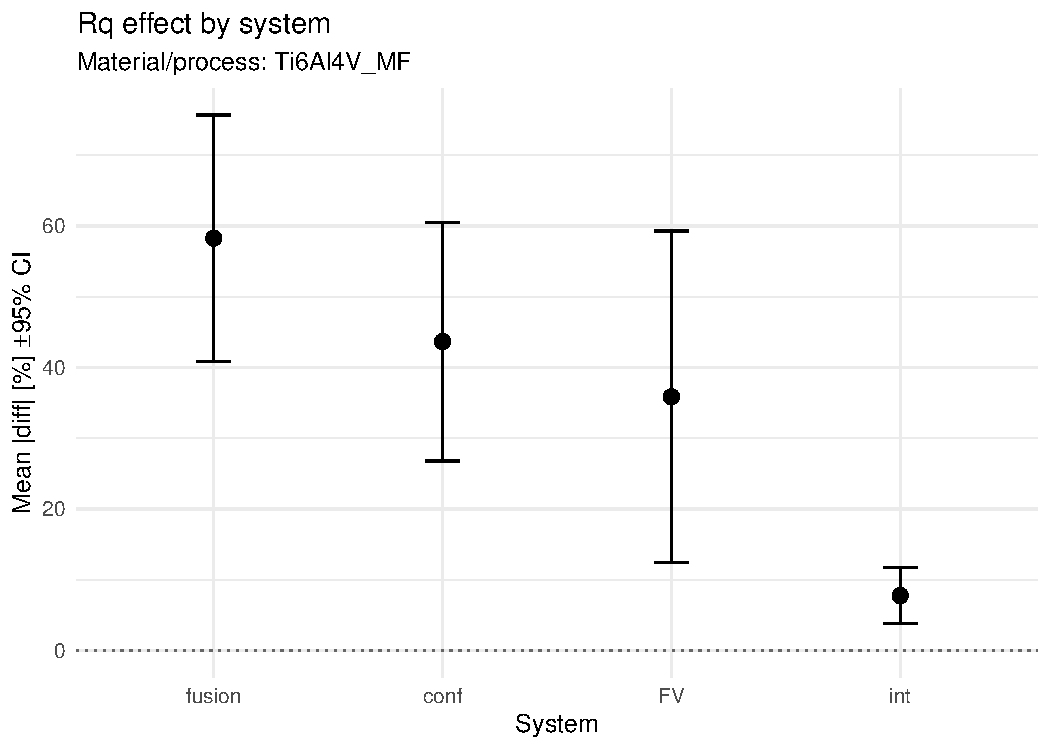
\includegraphics[width=0.95\linewidth]{../plots/rq_abs_ti6al4v_mf_effects_by_system.pdf}
\caption[Rq: main effects of system on |diff|(\%) for Ti6Al4V after finish milling]{$R_q$: main effects of system on $|\mathrm{diff}|(\%)$ for Ti6Al4V after finish milling}
\end{figure}
\clearpage

\begin{figure}[p]\centering
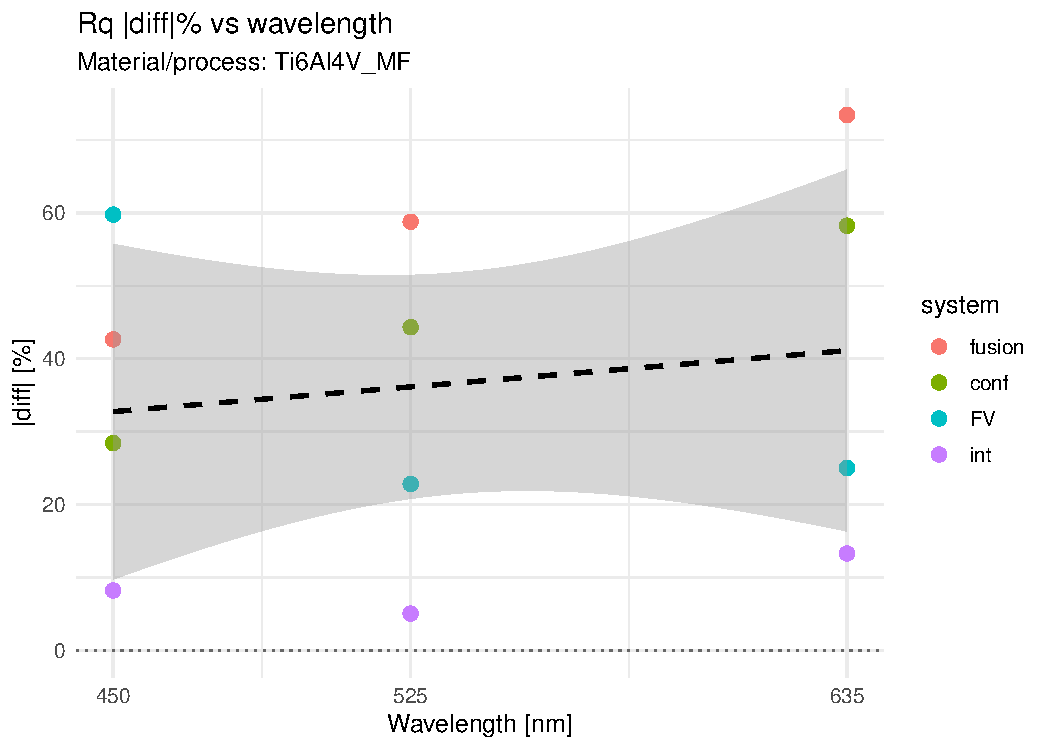
\includegraphics[width=0.95\linewidth]{../plots/rq_abs_ti6al4v_mf_diff_vs_wavelength.pdf}
\caption[Rq: |diff|(\%) versus wavelength for Ti6Al4V after finish milling]{$R_q$: $|\mathrm{diff}|(\%)$ versus illumination wavelength for Ti6Al4V after finish milling with fitted screening lines}
\end{figure}
\clearpage

\begin{figure}[p]\centering
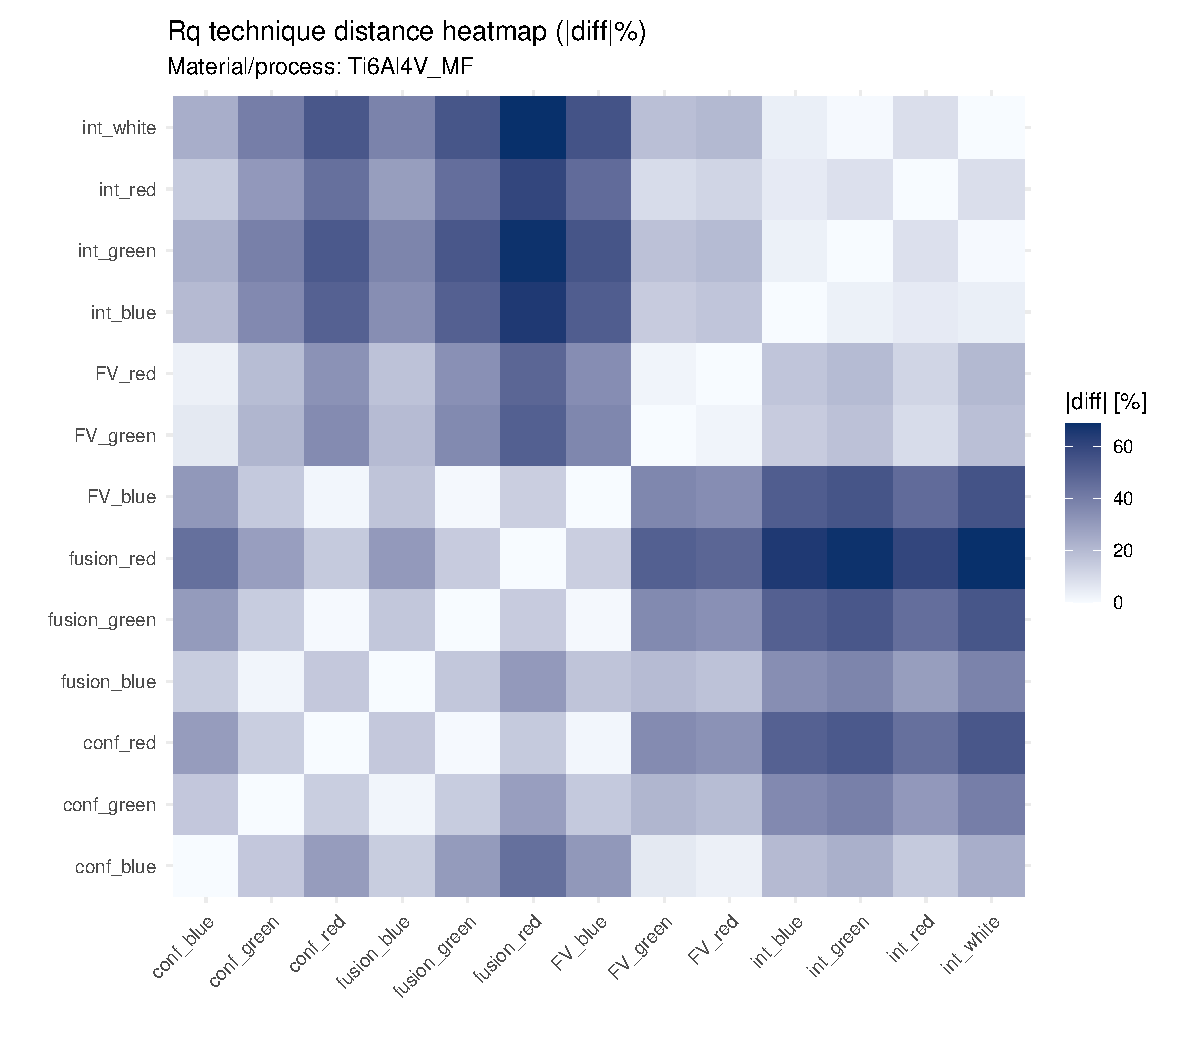
\includegraphics[width=0.95\linewidth]{../plots/rq_abs_ti6al4v_mf_tech_distance_heatmap.pdf}
\caption[Rq: technical-distance heatmap between systems for Ti6Al4V after finish milling]{$R_q$: technical-distance heatmap between systems for Ti6Al4V after finish milling, based on mean $|\mathrm{diff}|(\%)$}
\end{figure}
\clearpage

\subsection{Case B: C45 after wire EDM rough cutting (single-pass) (\texorpdfstring{$R_a$}{Ra})}
\begin{figure}[p]\centering
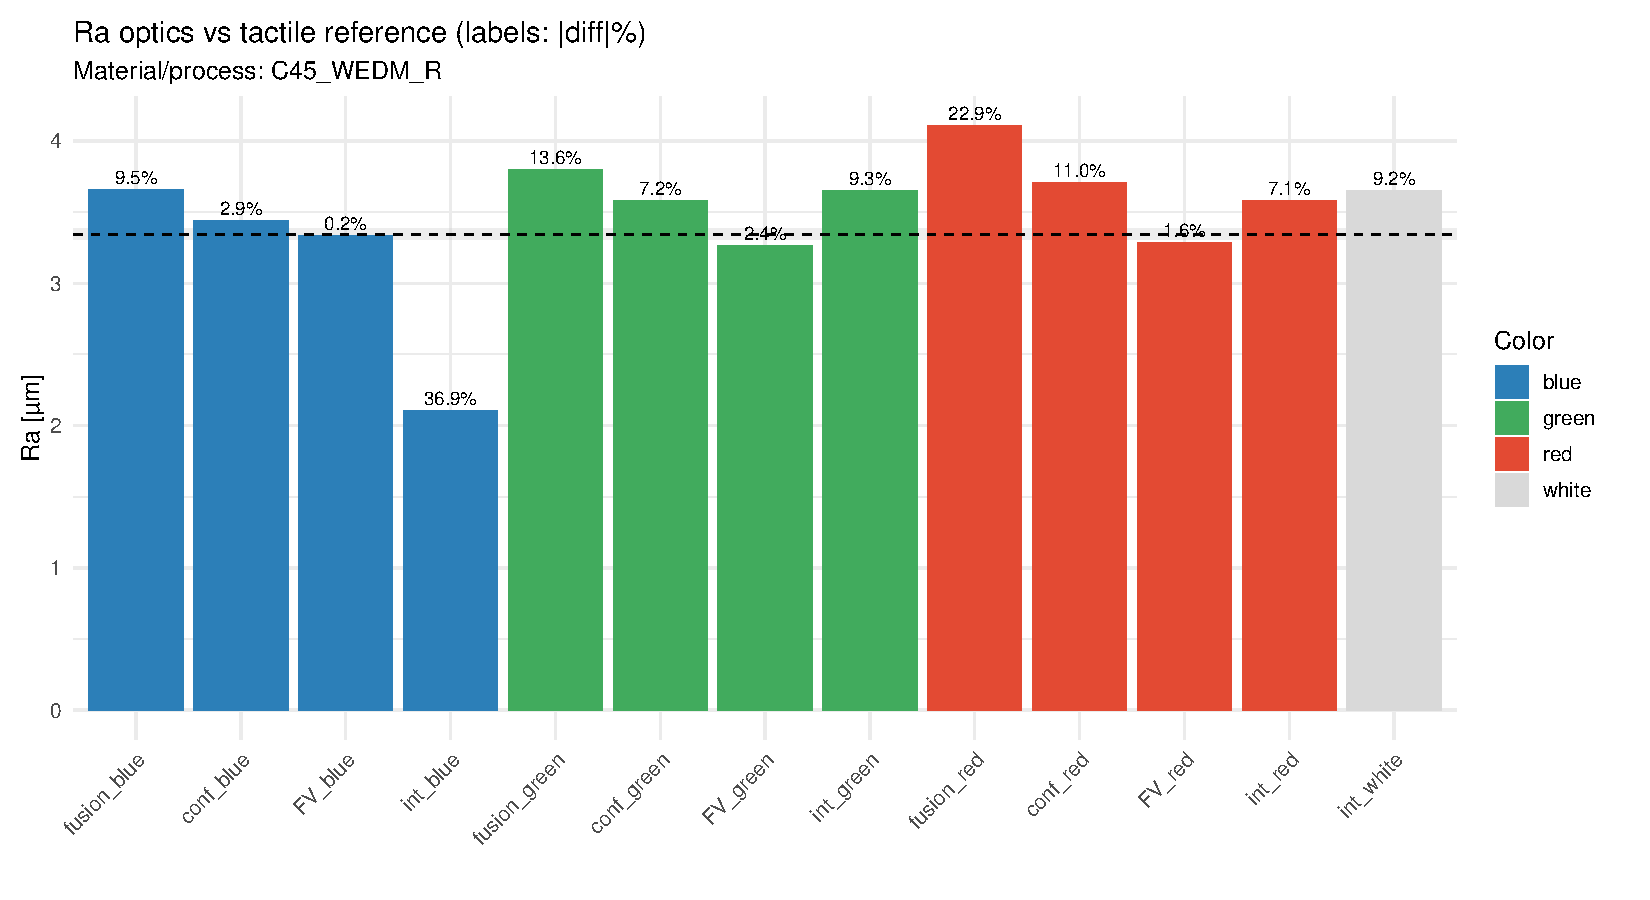
\includegraphics[width=0.95\linewidth]{../plots/ra_abs_c45_wedm_r_optics_vs_tactile.pdf}
\caption[Ra: optical--tactile comparison for C45 after wire EDM rough cutting (single-pass)]{$R_a$: optical--tactile comparison for C45 after wire EDM rough cutting (single-pass), summarising relative disagreement across systems}
\end{figure}
\clearpage

\begin{figure}[p]\centering
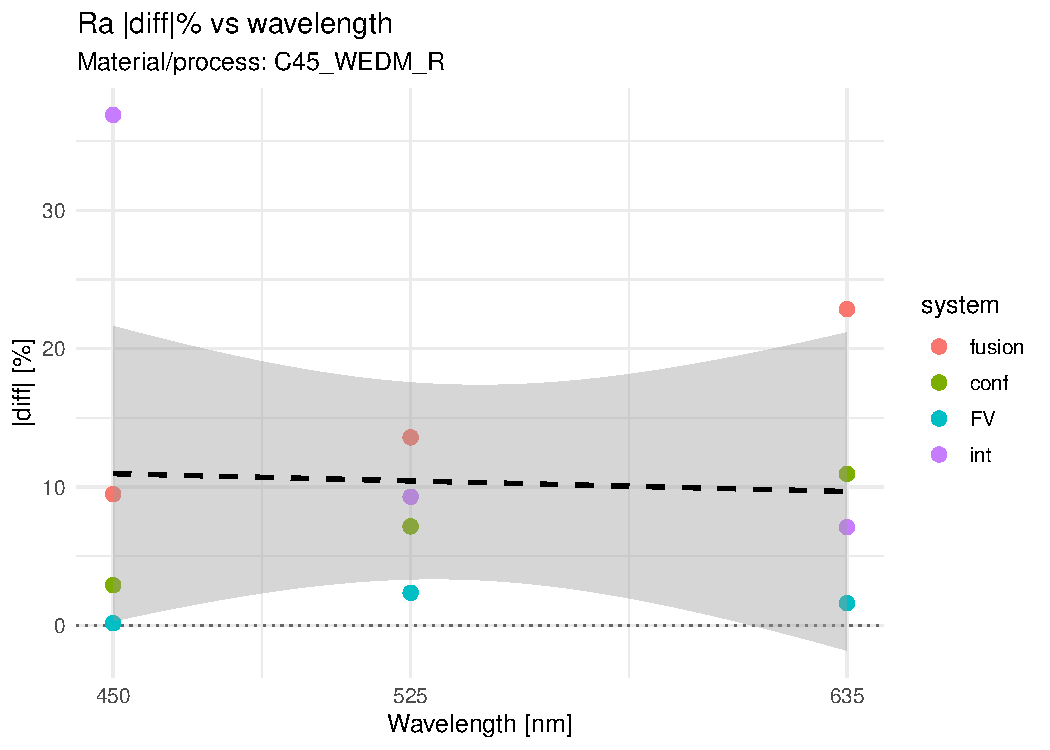
\includegraphics[width=0.95\linewidth]{../plots/ra_abs_c45_wedm_r_diff_vs_wavelength.pdf}
\caption[Ra: |diff|(\%) versus wavelength for C45 after wire EDM rough cutting (single-pass)]{$R_a$: $|\mathrm{diff}|(\%)$ versus illumination wavelength for C45 after wire EDM rough cutting (single-pass) with fitted screening lines}
\end{figure}
\clearpage

\end{document}
